
    \documentclass{article}
    \usepackage[a4paper, left=1cm, right=1cm, top=2cm, bottom=2cm]{geometry}
    \usepackage{hyperref} % für anklickbare Bezüge 
    \usepackage{tikz} % für MO-Schemata
    \usepackage{amsmath}
    \usepackage{physics}

    \setlength{\parindent}{0pt}
    \hypersetup{colorlinks=true, linkcolor=black, citecolor=black}% damit Referenzen nicht in PDF umklammert
    
    \begin{document}
    \pagestyle{empty}
    \tableofcontents 
    \newpage 
    \section{Orbitals And Their Symmetry}%Orbitale und deren Symmetrie 

%\includegraphics[scale=0.125]{img/DimerZOrbitalordnung-C6H5Cl-C2h-gesamt-MO-beiWW.pdf}
\vspace{2cm}
We use the following order of orbitals here (assuming degeneracy of LUMOs and HOMOs): 
$$
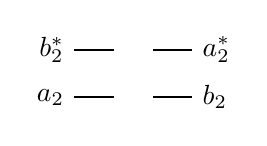
\begin{tikzpicture}[baseline={(current bounding box.center)}]
            % oberste MOs:
            \draw[thick] (0,0) -- (0.5,0)
                node[pos=0, left] {$b_2^{*}$}
                ;
            \draw[thick] (1,0) -- (1.5,0)
                node[pos=1, right] {$a_2^{*}$}
                ;
            % unterste MOs:
            \draw[thick] (0,-0.6) -- (0.5,-0.6)
                node[pos=0, left] {$a_2$}
                ;
            \draw[thick] (1,-0.6) -- (1.5,-0.6)
                node[pos=1, right] {$b_2$}
                ;
        
\end{tikzpicture}
$$
In the following, we will leave out the explicit labeling by orbital symmetry. Each monomer will simply be written as:
$$
\begin{tikzpicture}[baseline={(current bounding box.center)}]
            % oberste MOs:
            \draw[thick] (0,0) -- (0.5,0)
                %node[pos=0, left] {$b_2^{*}$}
                ;
            \draw[thick] (1,0) -- (1.5,0)
                %node[pos=1, right] {$a_2^{*}$}
                ;
            % unterste MOs:
            \draw[thick] (0,-0.6) -- (0.5,-0.6)
                %node[pos=0, left] {$a_2$}
                ;
            \draw[thick] (1,-0.6) -- (1.5,-0.6)
                %node[pos=1, right] {$b_2$}
                ;
        
\end{tikzpicture}
$$
where the character of the orbital is defined by its position. 

Dimer configurations will be written as their monomer occupations, by writing one monomer to the left and one to the right. The orbital order within the group of monomer orbitals follows the above mentioned definition. \vspace{2cm} The transformation of monomer orbitals into dimer orbitals is given by knowing the negative and positive linera combinations of monomer orbitals into dimer orbitals. Transforming this known equation system leads to: 
\begin{subequations}\begin{gather}
a_2^{*l} = +a_u^{*}+b_g^{*}  \\
b_2^{*l} = +a_g^{*}+b_u^{*}  \\
a_2^{l} = +a_{u}+b_g  \\
b_2^{l} = +a_{g}+b_u  \\
a_2^{*r} = +a_u^{*}-b_g^{*}  \\
b_2^{*r} = -a_g^{*}+b_u^{*}  \\
a_2^{r} = +a_{u}-b_g  \\
b_2^{r} = -a_{g}+b_u\end{gather}\end{subequations}
\newpage \section{Linear Combinations: 2 Monomer- / 1 Dimer-States}

\[+\left(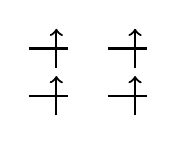
\begin{tikzpicture}[baseline={(current bounding box.center)}]
    % oberste MOs:
    \draw[thick] (0,0) -- (0.5,0); % erster Strich
    \draw[thick] (1,0) -- (1.5,0); % zweiter Strich
    % unterste MOs:
    \draw[thick] (0,-0.6) -- (0.5,-0.6); % dritter Strich
    \draw[thick] (1,-0.6) -- (1.5,-0.6); % vierter Strich
\draw[->, thick] (0.35, -0.25) -- (0.35, 0.25); 
\draw[->, thick] (1.35, -0.25) -- (1.35, 0.25); 
\draw[-> , thick] (0.35, -0.85) -- (0.35, -0.35); 
 \draw[-> , thick] (1.35, -0.85) -- (1.35, -0.35); 
\end{tikzpicture}\qquad 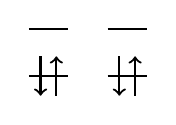
\begin{tikzpicture}[baseline={(current bounding box.center)}]
    % oberste MOs:
    \draw[thick] (0,0) -- (0.5,0); % erster Strich
    \draw[thick] (1,0) -- (1.5,0); % zweiter Strich
    % unterste MOs:
    \draw[thick] (0,-0.6) -- (0.5,-0.6); % dritter Strich
    \draw[thick] (1,-0.6) -- (1.5,-0.6); % vierter Strich
\draw[-> , thick] (0.35, -0.85) -- (0.35, -0.35); 
\draw[<- , thick] (0.15, -0.85) -- (0.15, -0.35); 
 \draw[-> , thick] (1.35, -0.85) -- (1.35, -0.35); 
\draw[<- , thick] (1.15, -0.85) -- (1.15, -0.35); 
\end{tikzpicture}\right)\]$$+ \underbrace{(b_2^{*l})\cdot (a_2^{*l})\cdot (a_2^{l})\cdot (b_2^{l})}_{\text{l: }a_1}\Rightarrow +\left|(b_2^{l}) \cdot (b_2^{*l}) \cdot (a_2^{l}) \cdot (a_2^{*l})\right|$$$$=+\left|(+a_{g}+b_u) \cdot (+a_g^{*}+b_u^{*}) \cdot (+a_{u}+b_g) \cdot (+a_u^{*}+b_g^{*})\right|$$\begin{multline*}
=+\left|\underbrace{a_{g} a_g^{*} a_{u} a_u^{*}}_{a_{g}}\right|+\left|\underbrace{a_{g} a_g^{*} a_{u} b_g^{*}}_{b_u}\right|+\left|\underbrace{a_{g} a_g^{*} b_g a_u^{*}}_{b_u}\right|+\left|\underbrace{a_{g} a_g^{*} b_g b_g^{*}}_{a_{g}}\right|\\
+\left|\underbrace{a_{g} b_u^{*} a_{u} a_u^{*}}_{b_u}\right|+\left|\underbrace{a_{g} b_u^{*} a_{u} b_g^{*}}_{a_{g}}\right|+\left|\underbrace{a_{g} b_u^{*} b_g a_u^{*}}_{a_{g}}\right|+\left|\underbrace{a_{g} b_u^{*} b_g b_g^{*}}_{b_u}\right|\\
+\left|\underbrace{b_u a_g^{*} a_{u} a_u^{*}}_{b_u}\right|+\left|\underbrace{b_u a_g^{*} a_{u} b_g^{*}}_{a_{g}}\right|+\left|\underbrace{b_u a_g^{*} b_g a_u^{*}}_{a_{g}}\right|+\left|\underbrace{b_u a_g^{*} b_g b_g^{*}}_{b_u}\right|\\
+\left|\underbrace{b_u b_u^{*} a_{u} a_u^{*}}_{a_{g}}\right|+\left|\underbrace{b_u b_u^{*} a_{u} b_g^{*}}_{b_u}\right|+\left|\underbrace{b_u b_u^{*} b_g a_u^{*}}_{b_u}\right|+\left|\underbrace{b_u b_u^{*} b_g b_g^{*}}_{a_{g}}\right|
\end{multline*}\begin{multline*}
=+\left|\underbrace{a_{g} a_g^{*} a_{u} a_u^{*}}_{a_{g}}\right|-\left|\underbrace{a_{g} a_g^{*} b_g^{*} a_{u}}_{b_u}\right|+\left|\underbrace{a_{g} a_g^{*} b_g a_u^{*}}_{b_u}\right|+\left|\underbrace{a_{g} a_g^{*} b_g b_g^{*}}_{a_{g}}\right|\\
+\left|\underbrace{a_{g} b_u^{*} a_{u} a_u^{*}}_{b_u}\right|+\left|\underbrace{a_{g} b_g^{*} b_u^{*} a_{u}}_{a_{g}}\right|-\left|\underbrace{a_{g} b_g b_u^{*} a_u^{*}}_{a_{g}}\right|+\left|\underbrace{a_{g} b_g b_g^{*} b_u^{*}}_{b_u}\right|\\
-\left|\underbrace{a_g^{*} b_u a_{u} a_u^{*}}_{b_u}\right|-\left|\underbrace{a_g^{*} b_g^{*} b_u a_{u}}_{a_{g}}\right|+\left|\underbrace{a_g^{*} b_g b_u a_u^{*}}_{a_{g}}\right|-\left|\underbrace{a_g^{*} b_g b_g^{*} b_u}_{b_u}\right|\\
+\left|\underbrace{b_u b_u^{*} a_{u} a_u^{*}}_{a_{g}}\right|-\left|\underbrace{b_g^{*} b_u b_u^{*} a_{u}}_{b_u}\right|+\left|\underbrace{b_g b_u b_u^{*} a_u^{*}}_{b_u}\right|+\left|\underbrace{b_g b_g^{*} b_u b_u^{*}}_{a_{g}}\right|
\end{multline*}(irreducible)\\ \\
\vspace{0.5cm}

\[+\left(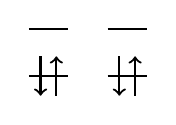
\begin{tikzpicture}[baseline={(current bounding box.center)}]
    % oberste MOs:
    \draw[thick] (0,0) -- (0.5,0); % erster Strich
    \draw[thick] (1,0) -- (1.5,0); % zweiter Strich
    % unterste MOs:
    \draw[thick] (0,-0.6) -- (0.5,-0.6); % dritter Strich
    \draw[thick] (1,-0.6) -- (1.5,-0.6); % vierter Strich
\draw[-> , thick] (0.35, -0.85) -- (0.35, -0.35); 
\draw[<- , thick] (0.15, -0.85) -- (0.15, -0.35); 
 \draw[-> , thick] (1.35, -0.85) -- (1.35, -0.35); 
\draw[<- , thick] (1.15, -0.85) -- (1.15, -0.35); 
\end{tikzpicture}\qquad 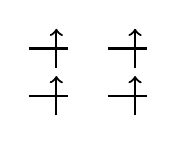
\begin{tikzpicture}[baseline={(current bounding box.center)}]
    % oberste MOs:
    \draw[thick] (0,0) -- (0.5,0); % erster Strich
    \draw[thick] (1,0) -- (1.5,0); % zweiter Strich
    % unterste MOs:
    \draw[thick] (0,-0.6) -- (0.5,-0.6); % dritter Strich
    \draw[thick] (1,-0.6) -- (1.5,-0.6); % vierter Strich
\draw[->, thick] (0.35, -0.25) -- (0.35, 0.25); 
\draw[->, thick] (1.35, -0.25) -- (1.35, 0.25); 
\draw[-> , thick] (0.35, -0.85) -- (0.35, -0.35); 
 \draw[-> , thick] (1.35, -0.85) -- (1.35, -0.35); 
\end{tikzpicture}\right)\]$$+ \underbrace{(b_2^{*r})\cdot (a_2^{*r})\cdot (a_2^{r})\cdot (b_2^{r})}_{\text{r: }a_1}\Rightarrow +\left|(b_2^{r}) \cdot (b_2^{*r}) \cdot (a_2^{r}) \cdot (a_2^{*r})\right|$$$$=+\left|(-a_{g}+b_u) \cdot (-a_g^{*}+b_u^{*}) \cdot (+a_{u}-b_g) \cdot (+a_u^{*}-b_g^{*})\right|$$\begin{multline*}
=+\left|\underbrace{a_{g} a_g^{*} a_{u} a_u^{*}}_{a_{g}}\right|-\left|\underbrace{a_{g} a_g^{*} a_{u} b_g^{*}}_{b_u}\right|-\left|\underbrace{a_{g} a_g^{*} b_g a_u^{*}}_{b_u}\right|+\left|\underbrace{a_{g} a_g^{*} b_g b_g^{*}}_{a_{g}}\right|\\
-\left|\underbrace{a_{g} b_u^{*} a_{u} a_u^{*}}_{b_u}\right|+\left|\underbrace{a_{g} b_u^{*} a_{u} b_g^{*}}_{a_{g}}\right|+\left|\underbrace{a_{g} b_u^{*} b_g a_u^{*}}_{a_{g}}\right|-\left|\underbrace{a_{g} b_u^{*} b_g b_g^{*}}_{b_u}\right|\\
-\left|\underbrace{b_u a_g^{*} a_{u} a_u^{*}}_{b_u}\right|+\left|\underbrace{b_u a_g^{*} a_{u} b_g^{*}}_{a_{g}}\right|+\left|\underbrace{b_u a_g^{*} b_g a_u^{*}}_{a_{g}}\right|-\left|\underbrace{b_u a_g^{*} b_g b_g^{*}}_{b_u}\right|\\
+\left|\underbrace{b_u b_u^{*} a_{u} a_u^{*}}_{a_{g}}\right|-\left|\underbrace{b_u b_u^{*} a_{u} b_g^{*}}_{b_u}\right|-\left|\underbrace{b_u b_u^{*} b_g a_u^{*}}_{b_u}\right|+\left|\underbrace{b_u b_u^{*} b_g b_g^{*}}_{a_{g}}\right|
\end{multline*}\begin{multline*}
=+\left|\underbrace{a_{g} a_g^{*} a_{u} a_u^{*}}_{a_{g}}\right|+\left|\underbrace{a_{g} a_g^{*} b_g^{*} a_{u}}_{b_u}\right|-\left|\underbrace{a_{g} a_g^{*} b_g a_u^{*}}_{b_u}\right|+\left|\underbrace{a_{g} a_g^{*} b_g b_g^{*}}_{a_{g}}\right|\\
-\left|\underbrace{a_{g} b_u^{*} a_{u} a_u^{*}}_{b_u}\right|+\left|\underbrace{a_{g} b_g^{*} b_u^{*} a_{u}}_{a_{g}}\right|-\left|\underbrace{a_{g} b_g b_u^{*} a_u^{*}}_{a_{g}}\right|-\left|\underbrace{a_{g} b_g b_g^{*} b_u^{*}}_{b_u}\right|\\
+\left|\underbrace{a_g^{*} b_u a_{u} a_u^{*}}_{b_u}\right|-\left|\underbrace{a_g^{*} b_g^{*} b_u a_{u}}_{a_{g}}\right|+\left|\underbrace{a_g^{*} b_g b_u a_u^{*}}_{a_{g}}\right|+\left|\underbrace{a_g^{*} b_g b_g^{*} b_u}_{b_u}\right|\\
+\left|\underbrace{b_u b_u^{*} a_{u} a_u^{*}}_{a_{g}}\right|+\left|\underbrace{b_g^{*} b_u b_u^{*} a_{u}}_{b_u}\right|-\left|\underbrace{b_g b_u b_u^{*} a_u^{*}}_{b_u}\right|+\left|\underbrace{b_g b_g^{*} b_u b_u^{*}}_{a_{g}}\right|
\end{multline*}(irreducible)\\ \\
\hrule\newpage 


\[+\left(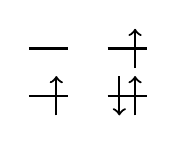
\begin{tikzpicture}[baseline={(current bounding box.center)}]
    % oberste MOs:
    \draw[thick] (0,0) -- (0.5,0); % erster Strich
    \draw[thick] (1,0) -- (1.5,0); % zweiter Strich
    % unterste MOs:
    \draw[thick] (0,-0.6) -- (0.5,-0.6); % dritter Strich
    \draw[thick] (1,-0.6) -- (1.5,-0.6); % vierter Strich
\draw[->, thick] (1.35, -0.25) -- (1.35, 0.25); 
\draw[-> , thick] (0.35, -0.85) -- (0.35, -0.35); 
 \draw[-> , thick] (1.35, -0.85) -- (1.35, -0.35); 
\draw[<- , thick] (1.15, -0.85) -- (1.15, -0.35); 
\end{tikzpicture}\qquad 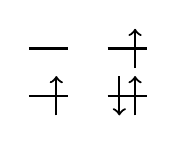
\begin{tikzpicture}[baseline={(current bounding box.center)}]
    % oberste MOs:
    \draw[thick] (0,0) -- (0.5,0); % erster Strich
    \draw[thick] (1,0) -- (1.5,0); % zweiter Strich
    % unterste MOs:
    \draw[thick] (0,-0.6) -- (0.5,-0.6); % dritter Strich
    \draw[thick] (1,-0.6) -- (1.5,-0.6); % vierter Strich
\draw[->, thick] (1.35, -0.25) -- (1.35, 0.25); 
\draw[-> , thick] (0.35, -0.85) -- (0.35, -0.35); 
 \draw[-> , thick] (1.35, -0.85) -- (1.35, -0.35); 
\draw[<- , thick] (1.15, -0.85) -- (1.15, -0.35); 
\end{tikzpicture}\right)\]$$+ \underbrace{(a_2^{*l})\cdot (a_2^{l})}_{\text{l: }a_1}\cdot \underbrace{(a_2^{*r})\cdot (a_2^{r})}_{\text{r: }a_1}\Rightarrow +\left|(a_2^{l}) \cdot (a_2^{r}) \cdot (a_2^{*l}) \cdot (a_2^{*r})\right|$$$$=+\left|(+a_{u}+b_g) \cdot (+a_{u}-b_g) \cdot (+a_u^{*}+b_g^{*}) \cdot (+a_u^{*}-b_g^{*})\right|$$\begin{multline*}
=+\left|\underbrace{a_{u} b_g a_u^{*} b_g^{*}}_{a_{g}}\right|-\left|\underbrace{a_{u} b_g b_g^{*} a_u^{*}}_{a_{g}}\right|-\left|\underbrace{b_g a_{u} a_u^{*} b_g^{*}}_{a_{g}}\right|+\left|\underbrace{b_g a_{u} b_g^{*} a_u^{*}}_{a_{g}}\right|\\
\end{multline*}\begin{multline*}
=-\left|\underbrace{b_g b_g^{*} a_{u} a_u^{*}}_{a_{g}}\right|-\left|\underbrace{b_g b_g^{*} a_{u} a_u^{*}}_{a_{g}}\right|-\left|\underbrace{b_g b_g^{*} a_{u} a_u^{*}}_{a_{g}}\right|-\left|\underbrace{b_g b_g^{*} a_{u} a_u^{*}}_{a_{g}}\right|\\
\end{multline*}summarized:\begin{multline*}
=-4\left|\underbrace{b_g b_g^{*} a_{u} a_u^{*}}_{a_{g}}\right|
\end{multline*}\\ \\
\hrule\newpage 


\[+\left(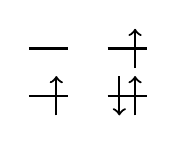
\begin{tikzpicture}[baseline={(current bounding box.center)}]
    % oberste MOs:
    \draw[thick] (0,0) -- (0.5,0); % erster Strich
    \draw[thick] (1,0) -- (1.5,0); % zweiter Strich
    % unterste MOs:
    \draw[thick] (0,-0.6) -- (0.5,-0.6); % dritter Strich
    \draw[thick] (1,-0.6) -- (1.5,-0.6); % vierter Strich
\draw[->, thick] (1.35, -0.25) -- (1.35, 0.25); 
\draw[-> , thick] (0.35, -0.85) -- (0.35, -0.35); 
 \draw[-> , thick] (1.35, -0.85) -- (1.35, -0.35); 
\draw[<- , thick] (1.15, -0.85) -- (1.15, -0.35); 
\end{tikzpicture}\qquad 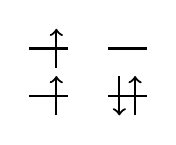
\begin{tikzpicture}[baseline={(current bounding box.center)}]
    % oberste MOs:
    \draw[thick] (0,0) -- (0.5,0); % erster Strich
    \draw[thick] (1,0) -- (1.5,0); % zweiter Strich
    % unterste MOs:
    \draw[thick] (0,-0.6) -- (0.5,-0.6); % dritter Strich
    \draw[thick] (1,-0.6) -- (1.5,-0.6); % vierter Strich
\draw[->, thick] (0.35, -0.25) -- (0.35, 0.25); 
\draw[-> , thick] (0.35, -0.85) -- (0.35, -0.35); 
 \draw[-> , thick] (1.35, -0.85) -- (1.35, -0.35); 
\draw[<- , thick] (1.15, -0.85) -- (1.15, -0.35); 
\end{tikzpicture}\right)\]$$+ \underbrace{(a_2^{*l})\cdot (a_2^{l})}_{\text{l: }a_1}\cdot \underbrace{(b_2^{*r})\cdot (a_2^{r})}_{\text{r: }b_1}\Rightarrow +\left|(b_2^{*r}) \cdot (a_2^{l}) \cdot (a_2^{r}) \cdot (a_2^{*l})\right|$$$$=+\left|(-a_g^{*}+b_u^{*}) \cdot (+a_{u}+b_g) \cdot (+a_{u}-b_g) \cdot (+a_u^{*}+b_g^{*})\right|$$\begin{multline*}
=+\left|\underbrace{a_g^{*} a_{u} b_g a_u^{*}}_{b_g}\right|+\left|\underbrace{a_g^{*} a_{u} b_g b_g^{*}}_{a_{u}}\right|-\left|\underbrace{a_g^{*} b_g a_{u} a_u^{*}}_{b_g}\right|-\left|\underbrace{a_g^{*} b_g a_{u} b_g^{*}}_{a_{u}}\right|\\
-\left|\underbrace{b_u^{*} a_{u} b_g a_u^{*}}_{a_{u}}\right|-\left|\underbrace{b_u^{*} a_{u} b_g b_g^{*}}_{b_g}\right|+\left|\underbrace{b_u^{*} b_g a_{u} a_u^{*}}_{a_{u}}\right|+\left|\underbrace{b_u^{*} b_g a_{u} b_g^{*}}_{b_g}\right|\\
\end{multline*}\begin{multline*}
=-\left|\underbrace{a_g^{*} b_g a_{u} a_u^{*}}_{b_g}\right|+\left|\underbrace{a_g^{*} b_g b_g^{*} a_{u}}_{a_{u}}\right|-\left|\underbrace{a_g^{*} b_g a_{u} a_u^{*}}_{b_g}\right|+\left|\underbrace{a_g^{*} b_g b_g^{*} a_{u}}_{a_{u}}\right|\\
-\left|\underbrace{b_g b_u^{*} a_{u} a_u^{*}}_{a_{u}}\right|-\left|\underbrace{b_g b_g^{*} b_u^{*} a_{u}}_{b_g}\right|-\left|\underbrace{b_g b_u^{*} a_{u} a_u^{*}}_{a_{u}}\right|-\left|\underbrace{b_g b_g^{*} b_u^{*} a_{u}}_{b_g}\right|\\
\end{multline*}summarized:\begin{multline*}
=-2\left|\underbrace{a_g^{*} b_g a_{u} a_u^{*}}_{b_g}\right|+2\left|\underbrace{a_g^{*} b_g b_g^{*} a_{u}}_{a_{u}}\right|-2\left|\underbrace{b_g b_u^{*} a_{u} a_u^{*}}_{a_{u}}\right|-2\left|\underbrace{b_g b_g^{*} b_u^{*} a_{u}}_{b_g}\right|\\
\end{multline*}\\ \\
\vspace{0.5cm}

\[+\left(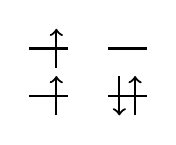
\begin{tikzpicture}[baseline={(current bounding box.center)}]
    % oberste MOs:
    \draw[thick] (0,0) -- (0.5,0); % erster Strich
    \draw[thick] (1,0) -- (1.5,0); % zweiter Strich
    % unterste MOs:
    \draw[thick] (0,-0.6) -- (0.5,-0.6); % dritter Strich
    \draw[thick] (1,-0.6) -- (1.5,-0.6); % vierter Strich
\draw[->, thick] (0.35, -0.25) -- (0.35, 0.25); 
\draw[-> , thick] (0.35, -0.85) -- (0.35, -0.35); 
 \draw[-> , thick] (1.35, -0.85) -- (1.35, -0.35); 
\draw[<- , thick] (1.15, -0.85) -- (1.15, -0.35); 
\end{tikzpicture}\qquad 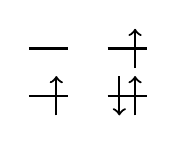
\begin{tikzpicture}[baseline={(current bounding box.center)}]
    % oberste MOs:
    \draw[thick] (0,0) -- (0.5,0); % erster Strich
    \draw[thick] (1,0) -- (1.5,0); % zweiter Strich
    % unterste MOs:
    \draw[thick] (0,-0.6) -- (0.5,-0.6); % dritter Strich
    \draw[thick] (1,-0.6) -- (1.5,-0.6); % vierter Strich
\draw[->, thick] (1.35, -0.25) -- (1.35, 0.25); 
\draw[-> , thick] (0.35, -0.85) -- (0.35, -0.35); 
 \draw[-> , thick] (1.35, -0.85) -- (1.35, -0.35); 
\draw[<- , thick] (1.15, -0.85) -- (1.15, -0.35); 
\end{tikzpicture}\right)\]$$+ \underbrace{(b_2^{*l})\cdot (a_2^{l})}_{\text{l: }b_1}\cdot \underbrace{(a_2^{*r})\cdot (a_2^{r})}_{\text{r: }a_1}\Rightarrow +\left|(b_2^{*l}) \cdot (a_2^{l}) \cdot (a_2^{r}) \cdot (a_2^{*r})\right|$$$$=+\left|(+a_g^{*}+b_u^{*}) \cdot (+a_{u}+b_g) \cdot (+a_{u}-b_g) \cdot (+a_u^{*}-b_g^{*})\right|$$\begin{multline*}
=-\left|\underbrace{a_g^{*} a_{u} b_g a_u^{*}}_{b_g}\right|+\left|\underbrace{a_g^{*} a_{u} b_g b_g^{*}}_{a_{u}}\right|+\left|\underbrace{a_g^{*} b_g a_{u} a_u^{*}}_{b_g}\right|-\left|\underbrace{a_g^{*} b_g a_{u} b_g^{*}}_{a_{u}}\right|\\
-\left|\underbrace{b_u^{*} a_{u} b_g a_u^{*}}_{a_{u}}\right|+\left|\underbrace{b_u^{*} a_{u} b_g b_g^{*}}_{b_g}\right|+\left|\underbrace{b_u^{*} b_g a_{u} a_u^{*}}_{a_{u}}\right|-\left|\underbrace{b_u^{*} b_g a_{u} b_g^{*}}_{b_g}\right|\\
\end{multline*}\begin{multline*}
=+\left|\underbrace{a_g^{*} b_g a_{u} a_u^{*}}_{b_g}\right|+\left|\underbrace{a_g^{*} b_g b_g^{*} a_{u}}_{a_{u}}\right|+\left|\underbrace{a_g^{*} b_g a_{u} a_u^{*}}_{b_g}\right|+\left|\underbrace{a_g^{*} b_g b_g^{*} a_{u}}_{a_{u}}\right|\\
-\left|\underbrace{b_g b_u^{*} a_{u} a_u^{*}}_{a_{u}}\right|+\left|\underbrace{b_g b_g^{*} b_u^{*} a_{u}}_{b_g}\right|-\left|\underbrace{b_g b_u^{*} a_{u} a_u^{*}}_{a_{u}}\right|+\left|\underbrace{b_g b_g^{*} b_u^{*} a_{u}}_{b_g}\right|\\
\end{multline*}summarized:\begin{multline*}
=+2\left|\underbrace{a_g^{*} b_g a_{u} a_u^{*}}_{b_g}\right|+2\left|\underbrace{a_g^{*} b_g b_g^{*} a_{u}}_{a_{u}}\right|-2\left|\underbrace{b_g b_u^{*} a_{u} a_u^{*}}_{a_{u}}\right|+2\left|\underbrace{b_g b_g^{*} b_u^{*} a_{u}}_{b_g}\right|\\
\end{multline*}\\ \\
\hrule\newpage 


\[+\left(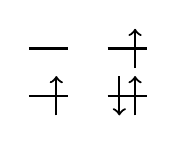
\begin{tikzpicture}[baseline={(current bounding box.center)}]
    % oberste MOs:
    \draw[thick] (0,0) -- (0.5,0); % erster Strich
    \draw[thick] (1,0) -- (1.5,0); % zweiter Strich
    % unterste MOs:
    \draw[thick] (0,-0.6) -- (0.5,-0.6); % dritter Strich
    \draw[thick] (1,-0.6) -- (1.5,-0.6); % vierter Strich
\draw[->, thick] (1.35, -0.25) -- (1.35, 0.25); 
\draw[-> , thick] (0.35, -0.85) -- (0.35, -0.35); 
 \draw[-> , thick] (1.35, -0.85) -- (1.35, -0.35); 
\draw[<- , thick] (1.15, -0.85) -- (1.15, -0.35); 
\end{tikzpicture}\qquad 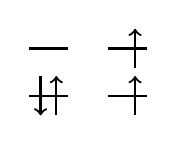
\begin{tikzpicture}[baseline={(current bounding box.center)}]
    % oberste MOs:
    \draw[thick] (0,0) -- (0.5,0); % erster Strich
    \draw[thick] (1,0) -- (1.5,0); % zweiter Strich
    % unterste MOs:
    \draw[thick] (0,-0.6) -- (0.5,-0.6); % dritter Strich
    \draw[thick] (1,-0.6) -- (1.5,-0.6); % vierter Strich
\draw[->, thick] (1.35, -0.25) -- (1.35, 0.25); 
\draw[-> , thick] (0.35, -0.85) -- (0.35, -0.35); 
\draw[<- , thick] (0.15, -0.85) -- (0.15, -0.35); 
 \draw[-> , thick] (1.35, -0.85) -- (1.35, -0.35); 
\end{tikzpicture}\right)\]$$+ \underbrace{(a_2^{*l})\cdot (a_2^{l})}_{\text{l: }a_1}\cdot \underbrace{(a_2^{*r})\cdot (b_2^{r})}_{\text{r: }b_1}\Rightarrow +\left|(b_2^{r}) \cdot (a_2^{l}) \cdot (a_2^{*l}) \cdot (a_2^{*r})\right|$$$$=+\left|(-a_{g}+b_u) \cdot (+a_{u}+b_g) \cdot (+a_u^{*}+b_g^{*}) \cdot (+a_u^{*}-b_g^{*})\right|$$\begin{multline*}
=+\left|\underbrace{a_{g} a_{u} a_u^{*} b_g^{*}}_{b_g}\right|-\left|\underbrace{a_{g} a_{u} b_g^{*} a_u^{*}}_{b_g}\right|+\left|\underbrace{a_{g} b_g a_u^{*} b_g^{*}}_{a_{u}}\right|-\left|\underbrace{a_{g} b_g b_g^{*} a_u^{*}}_{a_{u}}\right|\\
-\left|\underbrace{b_u a_{u} a_u^{*} b_g^{*}}_{a_{u}}\right|+\left|\underbrace{b_u a_{u} b_g^{*} a_u^{*}}_{a_{u}}\right|-\left|\underbrace{b_u b_g a_u^{*} b_g^{*}}_{b_g}\right|+\left|\underbrace{b_u b_g b_g^{*} a_u^{*}}_{b_g}\right|\\
\end{multline*}\begin{multline*}
=+\left|\underbrace{a_{g} b_g^{*} a_{u} a_u^{*}}_{b_g}\right|+\left|\underbrace{a_{g} b_g^{*} a_{u} a_u^{*}}_{b_g}\right|-\left|\underbrace{a_{g} b_g b_g^{*} a_u^{*}}_{a_{u}}\right|-\left|\underbrace{a_{g} b_g b_g^{*} a_u^{*}}_{a_{u}}\right|\\
+\left|\underbrace{b_g^{*} b_u a_{u} a_u^{*}}_{a_{u}}\right|+\left|\underbrace{b_g^{*} b_u a_{u} a_u^{*}}_{a_{u}}\right|+\left|\underbrace{b_g b_g^{*} b_u a_u^{*}}_{b_g}\right|+\left|\underbrace{b_g b_g^{*} b_u a_u^{*}}_{b_g}\right|\\
\end{multline*}summarized:\begin{multline*}
=+2\left|\underbrace{a_{g} b_g^{*} a_{u} a_u^{*}}_{b_g}\right|-2\left|\underbrace{a_{g} b_g b_g^{*} a_u^{*}}_{a_{u}}\right|+2\left|\underbrace{b_g^{*} b_u a_{u} a_u^{*}}_{a_{u}}\right|+2\left|\underbrace{b_g b_g^{*} b_u a_u^{*}}_{b_g}\right|\\
\end{multline*}\\ \\
\vspace{0.5cm}

\[+\left(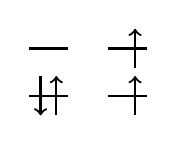
\begin{tikzpicture}[baseline={(current bounding box.center)}]
    % oberste MOs:
    \draw[thick] (0,0) -- (0.5,0); % erster Strich
    \draw[thick] (1,0) -- (1.5,0); % zweiter Strich
    % unterste MOs:
    \draw[thick] (0,-0.6) -- (0.5,-0.6); % dritter Strich
    \draw[thick] (1,-0.6) -- (1.5,-0.6); % vierter Strich
\draw[->, thick] (1.35, -0.25) -- (1.35, 0.25); 
\draw[-> , thick] (0.35, -0.85) -- (0.35, -0.35); 
\draw[<- , thick] (0.15, -0.85) -- (0.15, -0.35); 
 \draw[-> , thick] (1.35, -0.85) -- (1.35, -0.35); 
\end{tikzpicture}\qquad 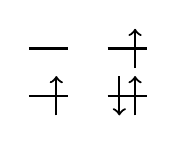
\begin{tikzpicture}[baseline={(current bounding box.center)}]
    % oberste MOs:
    \draw[thick] (0,0) -- (0.5,0); % erster Strich
    \draw[thick] (1,0) -- (1.5,0); % zweiter Strich
    % unterste MOs:
    \draw[thick] (0,-0.6) -- (0.5,-0.6); % dritter Strich
    \draw[thick] (1,-0.6) -- (1.5,-0.6); % vierter Strich
\draw[->, thick] (1.35, -0.25) -- (1.35, 0.25); 
\draw[-> , thick] (0.35, -0.85) -- (0.35, -0.35); 
 \draw[-> , thick] (1.35, -0.85) -- (1.35, -0.35); 
\draw[<- , thick] (1.15, -0.85) -- (1.15, -0.35); 
\end{tikzpicture}\right)\]$$+ \underbrace{(a_2^{*l})\cdot (b_2^{l})}_{\text{l: }b_1}\cdot \underbrace{(a_2^{*r})\cdot (a_2^{r})}_{\text{r: }a_1}\Rightarrow +\left|(b_2^{l}) \cdot (a_2^{r}) \cdot (a_2^{*l}) \cdot (a_2^{*r})\right|$$$$=+\left|(+a_{g}+b_u) \cdot (+a_{u}-b_g) \cdot (+a_u^{*}+b_g^{*}) \cdot (+a_u^{*}-b_g^{*})\right|$$\begin{multline*}
=-\left|\underbrace{a_{g} a_{u} a_u^{*} b_g^{*}}_{b_g}\right|+\left|\underbrace{a_{g} a_{u} b_g^{*} a_u^{*}}_{b_g}\right|+\left|\underbrace{a_{g} b_g a_u^{*} b_g^{*}}_{a_{u}}\right|-\left|\underbrace{a_{g} b_g b_g^{*} a_u^{*}}_{a_{u}}\right|\\
-\left|\underbrace{b_u a_{u} a_u^{*} b_g^{*}}_{a_{u}}\right|+\left|\underbrace{b_u a_{u} b_g^{*} a_u^{*}}_{a_{u}}\right|+\left|\underbrace{b_u b_g a_u^{*} b_g^{*}}_{b_g}\right|-\left|\underbrace{b_u b_g b_g^{*} a_u^{*}}_{b_g}\right|\\
\end{multline*}\begin{multline*}
=-\left|\underbrace{a_{g} b_g^{*} a_{u} a_u^{*}}_{b_g}\right|-\left|\underbrace{a_{g} b_g^{*} a_{u} a_u^{*}}_{b_g}\right|-\left|\underbrace{a_{g} b_g b_g^{*} a_u^{*}}_{a_{u}}\right|-\left|\underbrace{a_{g} b_g b_g^{*} a_u^{*}}_{a_{u}}\right|\\
+\left|\underbrace{b_g^{*} b_u a_{u} a_u^{*}}_{a_{u}}\right|+\left|\underbrace{b_g^{*} b_u a_{u} a_u^{*}}_{a_{u}}\right|-\left|\underbrace{b_g b_g^{*} b_u a_u^{*}}_{b_g}\right|-\left|\underbrace{b_g b_g^{*} b_u a_u^{*}}_{b_g}\right|\\
\end{multline*}summarized:\begin{multline*}
=-2\left|\underbrace{a_{g} b_g^{*} a_{u} a_u^{*}}_{b_g}\right|-2\left|\underbrace{a_{g} b_g b_g^{*} a_u^{*}}_{a_{u}}\right|+2\left|\underbrace{b_g^{*} b_u a_{u} a_u^{*}}_{a_{u}}\right|-2\left|\underbrace{b_g b_g^{*} b_u a_u^{*}}_{b_g}\right|\\
\end{multline*}\\ \\
\hrule\newpage 


\[+\left(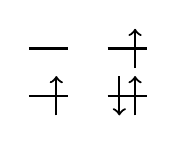
\begin{tikzpicture}[baseline={(current bounding box.center)}]
    % oberste MOs:
    \draw[thick] (0,0) -- (0.5,0); % erster Strich
    \draw[thick] (1,0) -- (1.5,0); % zweiter Strich
    % unterste MOs:
    \draw[thick] (0,-0.6) -- (0.5,-0.6); % dritter Strich
    \draw[thick] (1,-0.6) -- (1.5,-0.6); % vierter Strich
\draw[->, thick] (1.35, -0.25) -- (1.35, 0.25); 
\draw[-> , thick] (0.35, -0.85) -- (0.35, -0.35); 
 \draw[-> , thick] (1.35, -0.85) -- (1.35, -0.35); 
\draw[<- , thick] (1.15, -0.85) -- (1.15, -0.35); 
\end{tikzpicture}\qquad 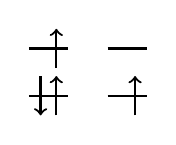
\begin{tikzpicture}[baseline={(current bounding box.center)}]
    % oberste MOs:
    \draw[thick] (0,0) -- (0.5,0); % erster Strich
    \draw[thick] (1,0) -- (1.5,0); % zweiter Strich
    % unterste MOs:
    \draw[thick] (0,-0.6) -- (0.5,-0.6); % dritter Strich
    \draw[thick] (1,-0.6) -- (1.5,-0.6); % vierter Strich
\draw[->, thick] (0.35, -0.25) -- (0.35, 0.25); 
\draw[-> , thick] (0.35, -0.85) -- (0.35, -0.35); 
\draw[<- , thick] (0.15, -0.85) -- (0.15, -0.35); 
 \draw[-> , thick] (1.35, -0.85) -- (1.35, -0.35); 
\end{tikzpicture}\right)\]$$+ \underbrace{(a_2^{*l})\cdot (a_2^{l})}_{\text{l: }a_1}\cdot \underbrace{(b_2^{*r})\cdot (b_2^{r})}_{\text{r: }a_1}\Rightarrow +\left|(b_2^{r}) \cdot (b_2^{*r}) \cdot (a_2^{l}) \cdot (a_2^{*l})\right|$$$$=+\left|(-a_{g}+b_u) \cdot (-a_g^{*}+b_u^{*}) \cdot (+a_{u}+b_g) \cdot (+a_u^{*}+b_g^{*})\right|$$\begin{multline*}
=+\left|\underbrace{a_{g} a_g^{*} a_{u} a_u^{*}}_{a_{g}}\right|+\left|\underbrace{a_{g} a_g^{*} a_{u} b_g^{*}}_{b_u}\right|+\left|\underbrace{a_{g} a_g^{*} b_g a_u^{*}}_{b_u}\right|+\left|\underbrace{a_{g} a_g^{*} b_g b_g^{*}}_{a_{g}}\right|\\
-\left|\underbrace{a_{g} b_u^{*} a_{u} a_u^{*}}_{b_u}\right|-\left|\underbrace{a_{g} b_u^{*} a_{u} b_g^{*}}_{a_{g}}\right|-\left|\underbrace{a_{g} b_u^{*} b_g a_u^{*}}_{a_{g}}\right|-\left|\underbrace{a_{g} b_u^{*} b_g b_g^{*}}_{b_u}\right|\\
-\left|\underbrace{b_u a_g^{*} a_{u} a_u^{*}}_{b_u}\right|-\left|\underbrace{b_u a_g^{*} a_{u} b_g^{*}}_{a_{g}}\right|-\left|\underbrace{b_u a_g^{*} b_g a_u^{*}}_{a_{g}}\right|-\left|\underbrace{b_u a_g^{*} b_g b_g^{*}}_{b_u}\right|\\
+\left|\underbrace{b_u b_u^{*} a_{u} a_u^{*}}_{a_{g}}\right|+\left|\underbrace{b_u b_u^{*} a_{u} b_g^{*}}_{b_u}\right|+\left|\underbrace{b_u b_u^{*} b_g a_u^{*}}_{b_u}\right|+\left|\underbrace{b_u b_u^{*} b_g b_g^{*}}_{a_{g}}\right|
\end{multline*}\begin{multline*}
=+\left|\underbrace{a_{g} a_g^{*} a_{u} a_u^{*}}_{a_{g}}\right|-\left|\underbrace{a_{g} a_g^{*} b_g^{*} a_{u}}_{b_u}\right|+\left|\underbrace{a_{g} a_g^{*} b_g a_u^{*}}_{b_u}\right|+\left|\underbrace{a_{g} a_g^{*} b_g b_g^{*}}_{a_{g}}\right|\\
-\left|\underbrace{a_{g} b_u^{*} a_{u} a_u^{*}}_{b_u}\right|-\left|\underbrace{a_{g} b_g^{*} b_u^{*} a_{u}}_{a_{g}}\right|+\left|\underbrace{a_{g} b_g b_u^{*} a_u^{*}}_{a_{g}}\right|-\left|\underbrace{a_{g} b_g b_g^{*} b_u^{*}}_{b_u}\right|\\
+\left|\underbrace{a_g^{*} b_u a_{u} a_u^{*}}_{b_u}\right|+\left|\underbrace{a_g^{*} b_g^{*} b_u a_{u}}_{a_{g}}\right|-\left|\underbrace{a_g^{*} b_g b_u a_u^{*}}_{a_{g}}\right|+\left|\underbrace{a_g^{*} b_g b_g^{*} b_u}_{b_u}\right|\\
+\left|\underbrace{b_u b_u^{*} a_{u} a_u^{*}}_{a_{g}}\right|-\left|\underbrace{b_g^{*} b_u b_u^{*} a_{u}}_{b_u}\right|+\left|\underbrace{b_g b_u b_u^{*} a_u^{*}}_{b_u}\right|+\left|\underbrace{b_g b_g^{*} b_u b_u^{*}}_{a_{g}}\right|
\end{multline*}(irreducible)\\ \\
\vspace{0.5cm}

\[+\left(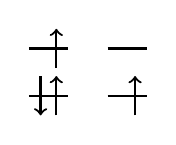
\begin{tikzpicture}[baseline={(current bounding box.center)}]
    % oberste MOs:
    \draw[thick] (0,0) -- (0.5,0); % erster Strich
    \draw[thick] (1,0) -- (1.5,0); % zweiter Strich
    % unterste MOs:
    \draw[thick] (0,-0.6) -- (0.5,-0.6); % dritter Strich
    \draw[thick] (1,-0.6) -- (1.5,-0.6); % vierter Strich
\draw[->, thick] (0.35, -0.25) -- (0.35, 0.25); 
\draw[-> , thick] (0.35, -0.85) -- (0.35, -0.35); 
\draw[<- , thick] (0.15, -0.85) -- (0.15, -0.35); 
 \draw[-> , thick] (1.35, -0.85) -- (1.35, -0.35); 
\end{tikzpicture}\qquad 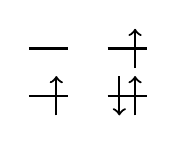
\begin{tikzpicture}[baseline={(current bounding box.center)}]
    % oberste MOs:
    \draw[thick] (0,0) -- (0.5,0); % erster Strich
    \draw[thick] (1,0) -- (1.5,0); % zweiter Strich
    % unterste MOs:
    \draw[thick] (0,-0.6) -- (0.5,-0.6); % dritter Strich
    \draw[thick] (1,-0.6) -- (1.5,-0.6); % vierter Strich
\draw[->, thick] (1.35, -0.25) -- (1.35, 0.25); 
\draw[-> , thick] (0.35, -0.85) -- (0.35, -0.35); 
 \draw[-> , thick] (1.35, -0.85) -- (1.35, -0.35); 
\draw[<- , thick] (1.15, -0.85) -- (1.15, -0.35); 
\end{tikzpicture}\right)\]$$+ \underbrace{(b_2^{*l})\cdot (b_2^{l})}_{\text{l: }a_1}\cdot \underbrace{(a_2^{*r})\cdot (a_2^{r})}_{\text{r: }a_1}\Rightarrow +\left|(b_2^{l}) \cdot (b_2^{*l}) \cdot (a_2^{r}) \cdot (a_2^{*r})\right|$$$$=+\left|(+a_{g}+b_u) \cdot (+a_g^{*}+b_u^{*}) \cdot (+a_{u}-b_g) \cdot (+a_u^{*}-b_g^{*})\right|$$\begin{multline*}
=+\left|\underbrace{a_{g} a_g^{*} a_{u} a_u^{*}}_{a_{g}}\right|-\left|\underbrace{a_{g} a_g^{*} a_{u} b_g^{*}}_{b_u}\right|-\left|\underbrace{a_{g} a_g^{*} b_g a_u^{*}}_{b_u}\right|+\left|\underbrace{a_{g} a_g^{*} b_g b_g^{*}}_{a_{g}}\right|\\
+\left|\underbrace{a_{g} b_u^{*} a_{u} a_u^{*}}_{b_u}\right|-\left|\underbrace{a_{g} b_u^{*} a_{u} b_g^{*}}_{a_{g}}\right|-\left|\underbrace{a_{g} b_u^{*} b_g a_u^{*}}_{a_{g}}\right|+\left|\underbrace{a_{g} b_u^{*} b_g b_g^{*}}_{b_u}\right|\\
+\left|\underbrace{b_u a_g^{*} a_{u} a_u^{*}}_{b_u}\right|-\left|\underbrace{b_u a_g^{*} a_{u} b_g^{*}}_{a_{g}}\right|-\left|\underbrace{b_u a_g^{*} b_g a_u^{*}}_{a_{g}}\right|+\left|\underbrace{b_u a_g^{*} b_g b_g^{*}}_{b_u}\right|\\
+\left|\underbrace{b_u b_u^{*} a_{u} a_u^{*}}_{a_{g}}\right|-\left|\underbrace{b_u b_u^{*} a_{u} b_g^{*}}_{b_u}\right|-\left|\underbrace{b_u b_u^{*} b_g a_u^{*}}_{b_u}\right|+\left|\underbrace{b_u b_u^{*} b_g b_g^{*}}_{a_{g}}\right|
\end{multline*}\begin{multline*}
=+\left|\underbrace{a_{g} a_g^{*} a_{u} a_u^{*}}_{a_{g}}\right|+\left|\underbrace{a_{g} a_g^{*} b_g^{*} a_{u}}_{b_u}\right|-\left|\underbrace{a_{g} a_g^{*} b_g a_u^{*}}_{b_u}\right|+\left|\underbrace{a_{g} a_g^{*} b_g b_g^{*}}_{a_{g}}\right|\\
+\left|\underbrace{a_{g} b_u^{*} a_{u} a_u^{*}}_{b_u}\right|-\left|\underbrace{a_{g} b_g^{*} b_u^{*} a_{u}}_{a_{g}}\right|+\left|\underbrace{a_{g} b_g b_u^{*} a_u^{*}}_{a_{g}}\right|+\left|\underbrace{a_{g} b_g b_g^{*} b_u^{*}}_{b_u}\right|\\
-\left|\underbrace{a_g^{*} b_u a_{u} a_u^{*}}_{b_u}\right|+\left|\underbrace{a_g^{*} b_g^{*} b_u a_{u}}_{a_{g}}\right|-\left|\underbrace{a_g^{*} b_g b_u a_u^{*}}_{a_{g}}\right|-\left|\underbrace{a_g^{*} b_g b_g^{*} b_u}_{b_u}\right|\\
+\left|\underbrace{b_u b_u^{*} a_{u} a_u^{*}}_{a_{g}}\right|+\left|\underbrace{b_g^{*} b_u b_u^{*} a_{u}}_{b_u}\right|-\left|\underbrace{b_g b_u b_u^{*} a_u^{*}}_{b_u}\right|+\left|\underbrace{b_g b_g^{*} b_u b_u^{*}}_{a_{g}}\right|
\end{multline*}(irreducible)\\ \\
\hrule\newpage 


\[+\left(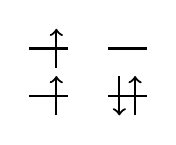
\begin{tikzpicture}[baseline={(current bounding box.center)}]
    % oberste MOs:
    \draw[thick] (0,0) -- (0.5,0); % erster Strich
    \draw[thick] (1,0) -- (1.5,0); % zweiter Strich
    % unterste MOs:
    \draw[thick] (0,-0.6) -- (0.5,-0.6); % dritter Strich
    \draw[thick] (1,-0.6) -- (1.5,-0.6); % vierter Strich
\draw[->, thick] (0.35, -0.25) -- (0.35, 0.25); 
\draw[-> , thick] (0.35, -0.85) -- (0.35, -0.35); 
 \draw[-> , thick] (1.35, -0.85) -- (1.35, -0.35); 
\draw[<- , thick] (1.15, -0.85) -- (1.15, -0.35); 
\end{tikzpicture}\qquad 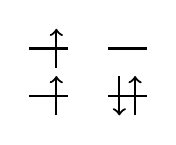
\begin{tikzpicture}[baseline={(current bounding box.center)}]
    % oberste MOs:
    \draw[thick] (0,0) -- (0.5,0); % erster Strich
    \draw[thick] (1,0) -- (1.5,0); % zweiter Strich
    % unterste MOs:
    \draw[thick] (0,-0.6) -- (0.5,-0.6); % dritter Strich
    \draw[thick] (1,-0.6) -- (1.5,-0.6); % vierter Strich
\draw[->, thick] (0.35, -0.25) -- (0.35, 0.25); 
\draw[-> , thick] (0.35, -0.85) -- (0.35, -0.35); 
 \draw[-> , thick] (1.35, -0.85) -- (1.35, -0.35); 
\draw[<- , thick] (1.15, -0.85) -- (1.15, -0.35); 
\end{tikzpicture}\right)\]$$+ \underbrace{(b_2^{*l})\cdot (a_2^{l})}_{\text{l: }b_1}\cdot \underbrace{(b_2^{*r})\cdot (a_2^{r})}_{\text{r: }b_1}\Rightarrow +\left|(b_2^{*l}) \cdot (b_2^{*r}) \cdot (a_2^{l}) \cdot (a_2^{r})\right|$$$$=+\left|(+a_g^{*}+b_u^{*}) \cdot (-a_g^{*}+b_u^{*}) \cdot (+a_{u}+b_g) \cdot (+a_{u}-b_g)\right|$$\begin{multline*}
=-\left|\underbrace{a_g^{*} b_u^{*} a_{u} b_g}_{a_{g}}\right|+\left|\underbrace{a_g^{*} b_u^{*} b_g a_{u}}_{a_{g}}\right|+\left|\underbrace{b_u^{*} a_g^{*} a_{u} b_g}_{a_{g}}\right|-\left|\underbrace{b_u^{*} a_g^{*} b_g a_{u}}_{a_{g}}\right|\\
\end{multline*}\begin{multline*}
=-\left|\underbrace{a_g^{*} b_g b_u^{*} a_{u}}_{a_{g}}\right|-\left|\underbrace{a_g^{*} b_g b_u^{*} a_{u}}_{a_{g}}\right|-\left|\underbrace{a_g^{*} b_g b_u^{*} a_{u}}_{a_{g}}\right|-\left|\underbrace{a_g^{*} b_g b_u^{*} a_{u}}_{a_{g}}\right|\\
\end{multline*}summarized:\begin{multline*}
=-4\left|\underbrace{a_g^{*} b_g b_u^{*} a_{u}}_{a_{g}}\right|
\end{multline*}\\ \\
\hrule\newpage 


\[+\left(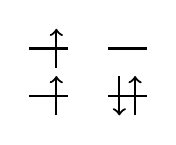
\begin{tikzpicture}[baseline={(current bounding box.center)}]
    % oberste MOs:
    \draw[thick] (0,0) -- (0.5,0); % erster Strich
    \draw[thick] (1,0) -- (1.5,0); % zweiter Strich
    % unterste MOs:
    \draw[thick] (0,-0.6) -- (0.5,-0.6); % dritter Strich
    \draw[thick] (1,-0.6) -- (1.5,-0.6); % vierter Strich
\draw[->, thick] (0.35, -0.25) -- (0.35, 0.25); 
\draw[-> , thick] (0.35, -0.85) -- (0.35, -0.35); 
 \draw[-> , thick] (1.35, -0.85) -- (1.35, -0.35); 
\draw[<- , thick] (1.15, -0.85) -- (1.15, -0.35); 
\end{tikzpicture}\qquad 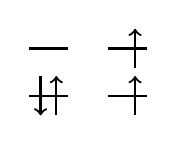
\begin{tikzpicture}[baseline={(current bounding box.center)}]
    % oberste MOs:
    \draw[thick] (0,0) -- (0.5,0); % erster Strich
    \draw[thick] (1,0) -- (1.5,0); % zweiter Strich
    % unterste MOs:
    \draw[thick] (0,-0.6) -- (0.5,-0.6); % dritter Strich
    \draw[thick] (1,-0.6) -- (1.5,-0.6); % vierter Strich
\draw[->, thick] (1.35, -0.25) -- (1.35, 0.25); 
\draw[-> , thick] (0.35, -0.85) -- (0.35, -0.35); 
\draw[<- , thick] (0.15, -0.85) -- (0.15, -0.35); 
 \draw[-> , thick] (1.35, -0.85) -- (1.35, -0.35); 
\end{tikzpicture}\right)\]$$+ \underbrace{(b_2^{*l})\cdot (a_2^{l})}_{\text{l: }b_1}\cdot \underbrace{(a_2^{*r})\cdot (b_2^{r})}_{\text{r: }b_1}\Rightarrow +\left|(b_2^{r}) \cdot (b_2^{*l}) \cdot (a_2^{l}) \cdot (a_2^{*r})\right|$$$$=+\left|(-a_{g}+b_u) \cdot (+a_g^{*}+b_u^{*}) \cdot (+a_{u}+b_g) \cdot (+a_u^{*}-b_g^{*})\right|$$\begin{multline*}
=-\left|\underbrace{a_{g} a_g^{*} a_{u} a_u^{*}}_{a_{g}}\right|+\left|\underbrace{a_{g} a_g^{*} a_{u} b_g^{*}}_{b_u}\right|-\left|\underbrace{a_{g} a_g^{*} b_g a_u^{*}}_{b_u}\right|+\left|\underbrace{a_{g} a_g^{*} b_g b_g^{*}}_{a_{g}}\right|\\
-\left|\underbrace{a_{g} b_u^{*} a_{u} a_u^{*}}_{b_u}\right|+\left|\underbrace{a_{g} b_u^{*} a_{u} b_g^{*}}_{a_{g}}\right|-\left|\underbrace{a_{g} b_u^{*} b_g a_u^{*}}_{a_{g}}\right|+\left|\underbrace{a_{g} b_u^{*} b_g b_g^{*}}_{b_u}\right|\\
+\left|\underbrace{b_u a_g^{*} a_{u} a_u^{*}}_{b_u}\right|-\left|\underbrace{b_u a_g^{*} a_{u} b_g^{*}}_{a_{g}}\right|+\left|\underbrace{b_u a_g^{*} b_g a_u^{*}}_{a_{g}}\right|-\left|\underbrace{b_u a_g^{*} b_g b_g^{*}}_{b_u}\right|\\
+\left|\underbrace{b_u b_u^{*} a_{u} a_u^{*}}_{a_{g}}\right|-\left|\underbrace{b_u b_u^{*} a_{u} b_g^{*}}_{b_u}\right|+\left|\underbrace{b_u b_u^{*} b_g a_u^{*}}_{b_u}\right|-\left|\underbrace{b_u b_u^{*} b_g b_g^{*}}_{a_{g}}\right|
\end{multline*}\begin{multline*}
=-\left|\underbrace{a_{g} a_g^{*} a_{u} a_u^{*}}_{a_{g}}\right|-\left|\underbrace{a_{g} a_g^{*} b_g^{*} a_{u}}_{b_u}\right|-\left|\underbrace{a_{g} a_g^{*} b_g a_u^{*}}_{b_u}\right|+\left|\underbrace{a_{g} a_g^{*} b_g b_g^{*}}_{a_{g}}\right|\\
-\left|\underbrace{a_{g} b_u^{*} a_{u} a_u^{*}}_{b_u}\right|+\left|\underbrace{a_{g} b_g^{*} b_u^{*} a_{u}}_{a_{g}}\right|+\left|\underbrace{a_{g} b_g b_u^{*} a_u^{*}}_{a_{g}}\right|+\left|\underbrace{a_{g} b_g b_g^{*} b_u^{*}}_{b_u}\right|\\
-\left|\underbrace{a_g^{*} b_u a_{u} a_u^{*}}_{b_u}\right|+\left|\underbrace{a_g^{*} b_g^{*} b_u a_{u}}_{a_{g}}\right|+\left|\underbrace{a_g^{*} b_g b_u a_u^{*}}_{a_{g}}\right|+\left|\underbrace{a_g^{*} b_g b_g^{*} b_u}_{b_u}\right|\\
+\left|\underbrace{b_u b_u^{*} a_{u} a_u^{*}}_{a_{g}}\right|+\left|\underbrace{b_g^{*} b_u b_u^{*} a_{u}}_{b_u}\right|+\left|\underbrace{b_g b_u b_u^{*} a_u^{*}}_{b_u}\right|-\left|\underbrace{b_g b_g^{*} b_u b_u^{*}}_{a_{g}}\right|
\end{multline*}(irreducible)\\ \\
\vspace{0.5cm}

\[+\left(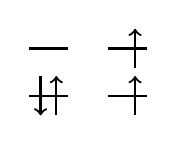
\begin{tikzpicture}[baseline={(current bounding box.center)}]
    % oberste MOs:
    \draw[thick] (0,0) -- (0.5,0); % erster Strich
    \draw[thick] (1,0) -- (1.5,0); % zweiter Strich
    % unterste MOs:
    \draw[thick] (0,-0.6) -- (0.5,-0.6); % dritter Strich
    \draw[thick] (1,-0.6) -- (1.5,-0.6); % vierter Strich
\draw[->, thick] (1.35, -0.25) -- (1.35, 0.25); 
\draw[-> , thick] (0.35, -0.85) -- (0.35, -0.35); 
\draw[<- , thick] (0.15, -0.85) -- (0.15, -0.35); 
 \draw[-> , thick] (1.35, -0.85) -- (1.35, -0.35); 
\end{tikzpicture}\qquad 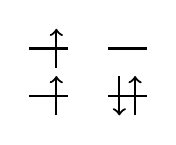
\begin{tikzpicture}[baseline={(current bounding box.center)}]
    % oberste MOs:
    \draw[thick] (0,0) -- (0.5,0); % erster Strich
    \draw[thick] (1,0) -- (1.5,0); % zweiter Strich
    % unterste MOs:
    \draw[thick] (0,-0.6) -- (0.5,-0.6); % dritter Strich
    \draw[thick] (1,-0.6) -- (1.5,-0.6); % vierter Strich
\draw[->, thick] (0.35, -0.25) -- (0.35, 0.25); 
\draw[-> , thick] (0.35, -0.85) -- (0.35, -0.35); 
 \draw[-> , thick] (1.35, -0.85) -- (1.35, -0.35); 
\draw[<- , thick] (1.15, -0.85) -- (1.15, -0.35); 
\end{tikzpicture}\right)\]$$+ \underbrace{(a_2^{*l})\cdot (b_2^{l})}_{\text{l: }b_1}\cdot \underbrace{(b_2^{*r})\cdot (a_2^{r})}_{\text{r: }b_1}\Rightarrow +\left|(b_2^{l}) \cdot (b_2^{*r}) \cdot (a_2^{r}) \cdot (a_2^{*l})\right|$$$$=+\left|(+a_{g}+b_u) \cdot (-a_g^{*}+b_u^{*}) \cdot (+a_{u}-b_g) \cdot (+a_u^{*}+b_g^{*})\right|$$\begin{multline*}
=-\left|\underbrace{a_{g} a_g^{*} a_{u} a_u^{*}}_{a_{g}}\right|-\left|\underbrace{a_{g} a_g^{*} a_{u} b_g^{*}}_{b_u}\right|+\left|\underbrace{a_{g} a_g^{*} b_g a_u^{*}}_{b_u}\right|+\left|\underbrace{a_{g} a_g^{*} b_g b_g^{*}}_{a_{g}}\right|\\
+\left|\underbrace{a_{g} b_u^{*} a_{u} a_u^{*}}_{b_u}\right|+\left|\underbrace{a_{g} b_u^{*} a_{u} b_g^{*}}_{a_{g}}\right|-\left|\underbrace{a_{g} b_u^{*} b_g a_u^{*}}_{a_{g}}\right|-\left|\underbrace{a_{g} b_u^{*} b_g b_g^{*}}_{b_u}\right|\\
-\left|\underbrace{b_u a_g^{*} a_{u} a_u^{*}}_{b_u}\right|-\left|\underbrace{b_u a_g^{*} a_{u} b_g^{*}}_{a_{g}}\right|+\left|\underbrace{b_u a_g^{*} b_g a_u^{*}}_{a_{g}}\right|+\left|\underbrace{b_u a_g^{*} b_g b_g^{*}}_{b_u}\right|\\
+\left|\underbrace{b_u b_u^{*} a_{u} a_u^{*}}_{a_{g}}\right|+\left|\underbrace{b_u b_u^{*} a_{u} b_g^{*}}_{b_u}\right|-\left|\underbrace{b_u b_u^{*} b_g a_u^{*}}_{b_u}\right|-\left|\underbrace{b_u b_u^{*} b_g b_g^{*}}_{a_{g}}\right|
\end{multline*}\begin{multline*}
=-\left|\underbrace{a_{g} a_g^{*} a_{u} a_u^{*}}_{a_{g}}\right|+\left|\underbrace{a_{g} a_g^{*} b_g^{*} a_{u}}_{b_u}\right|+\left|\underbrace{a_{g} a_g^{*} b_g a_u^{*}}_{b_u}\right|+\left|\underbrace{a_{g} a_g^{*} b_g b_g^{*}}_{a_{g}}\right|\\
+\left|\underbrace{a_{g} b_u^{*} a_{u} a_u^{*}}_{b_u}\right|+\left|\underbrace{a_{g} b_g^{*} b_u^{*} a_{u}}_{a_{g}}\right|+\left|\underbrace{a_{g} b_g b_u^{*} a_u^{*}}_{a_{g}}\right|-\left|\underbrace{a_{g} b_g b_g^{*} b_u^{*}}_{b_u}\right|\\
+\left|\underbrace{a_g^{*} b_u a_{u} a_u^{*}}_{b_u}\right|+\left|\underbrace{a_g^{*} b_g^{*} b_u a_{u}}_{a_{g}}\right|+\left|\underbrace{a_g^{*} b_g b_u a_u^{*}}_{a_{g}}\right|-\left|\underbrace{a_g^{*} b_g b_g^{*} b_u}_{b_u}\right|\\
+\left|\underbrace{b_u b_u^{*} a_{u} a_u^{*}}_{a_{g}}\right|-\left|\underbrace{b_g^{*} b_u b_u^{*} a_{u}}_{b_u}\right|-\left|\underbrace{b_g b_u b_u^{*} a_u^{*}}_{b_u}\right|-\left|\underbrace{b_g b_g^{*} b_u b_u^{*}}_{a_{g}}\right|
\end{multline*}(irreducible)\\ \\
\hrule\newpage 


\[+\left(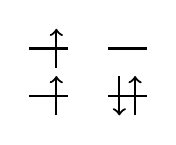
\begin{tikzpicture}[baseline={(current bounding box.center)}]
    % oberste MOs:
    \draw[thick] (0,0) -- (0.5,0); % erster Strich
    \draw[thick] (1,0) -- (1.5,0); % zweiter Strich
    % unterste MOs:
    \draw[thick] (0,-0.6) -- (0.5,-0.6); % dritter Strich
    \draw[thick] (1,-0.6) -- (1.5,-0.6); % vierter Strich
\draw[->, thick] (0.35, -0.25) -- (0.35, 0.25); 
\draw[-> , thick] (0.35, -0.85) -- (0.35, -0.35); 
 \draw[-> , thick] (1.35, -0.85) -- (1.35, -0.35); 
\draw[<- , thick] (1.15, -0.85) -- (1.15, -0.35); 
\end{tikzpicture}\qquad 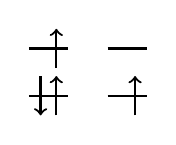
\begin{tikzpicture}[baseline={(current bounding box.center)}]
    % oberste MOs:
    \draw[thick] (0,0) -- (0.5,0); % erster Strich
    \draw[thick] (1,0) -- (1.5,0); % zweiter Strich
    % unterste MOs:
    \draw[thick] (0,-0.6) -- (0.5,-0.6); % dritter Strich
    \draw[thick] (1,-0.6) -- (1.5,-0.6); % vierter Strich
\draw[->, thick] (0.35, -0.25) -- (0.35, 0.25); 
\draw[-> , thick] (0.35, -0.85) -- (0.35, -0.35); 
\draw[<- , thick] (0.15, -0.85) -- (0.15, -0.35); 
 \draw[-> , thick] (1.35, -0.85) -- (1.35, -0.35); 
\end{tikzpicture}\right)\]$$+ \underbrace{(b_2^{*l})\cdot (a_2^{l})}_{\text{l: }b_1}\cdot \underbrace{(b_2^{*r})\cdot (b_2^{r})}_{\text{r: }a_1}\Rightarrow +\left|(b_2^{r}) \cdot (b_2^{*l}) \cdot (b_2^{*r}) \cdot (a_2^{l})\right|$$$$=+\left|(-a_{g}+b_u) \cdot (+a_g^{*}+b_u^{*}) \cdot (-a_g^{*}+b_u^{*}) \cdot (+a_{u}+b_g)\right|$$\begin{multline*}
=-\left|\underbrace{a_{g} a_g^{*} b_u^{*} a_{u}}_{b_g}\right|-\left|\underbrace{a_{g} a_g^{*} b_u^{*} b_g}_{a_{u}}\right|+\left|\underbrace{a_{g} b_u^{*} a_g^{*} a_{u}}_{b_g}\right|+\left|\underbrace{a_{g} b_u^{*} a_g^{*} b_g}_{a_{u}}\right|\\
+\left|\underbrace{b_u a_g^{*} b_u^{*} a_{u}}_{a_{u}}\right|+\left|\underbrace{b_u a_g^{*} b_u^{*} b_g}_{b_g}\right|-\left|\underbrace{b_u b_u^{*} a_g^{*} a_{u}}_{a_{u}}\right|-\left|\underbrace{b_u b_u^{*} a_g^{*} b_g}_{b_g}\right|\\
\end{multline*}\begin{multline*}
=-\left|\underbrace{a_{g} a_g^{*} b_u^{*} a_{u}}_{b_g}\right|+\left|\underbrace{a_{g} a_g^{*} b_g b_u^{*}}_{a_{u}}\right|-\left|\underbrace{a_{g} a_g^{*} b_u^{*} a_{u}}_{b_g}\right|+\left|\underbrace{a_{g} a_g^{*} b_g b_u^{*}}_{a_{u}}\right|\\
-\left|\underbrace{a_g^{*} b_u b_u^{*} a_{u}}_{a_{u}}\right|-\left|\underbrace{a_g^{*} b_g b_u b_u^{*}}_{b_g}\right|-\left|\underbrace{a_g^{*} b_u b_u^{*} a_{u}}_{a_{u}}\right|-\left|\underbrace{a_g^{*} b_g b_u b_u^{*}}_{b_g}\right|\\
\end{multline*}summarized:\begin{multline*}
=-2\left|\underbrace{a_{g} a_g^{*} b_u^{*} a_{u}}_{b_g}\right|+2\left|\underbrace{a_{g} a_g^{*} b_g b_u^{*}}_{a_{u}}\right|-2\left|\underbrace{a_g^{*} b_u b_u^{*} a_{u}}_{a_{u}}\right|-2\left|\underbrace{a_g^{*} b_g b_u b_u^{*}}_{b_g}\right|\\
\end{multline*}\\ \\
\vspace{0.5cm}

\[+\left(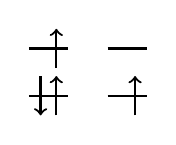
\begin{tikzpicture}[baseline={(current bounding box.center)}]
    % oberste MOs:
    \draw[thick] (0,0) -- (0.5,0); % erster Strich
    \draw[thick] (1,0) -- (1.5,0); % zweiter Strich
    % unterste MOs:
    \draw[thick] (0,-0.6) -- (0.5,-0.6); % dritter Strich
    \draw[thick] (1,-0.6) -- (1.5,-0.6); % vierter Strich
\draw[->, thick] (0.35, -0.25) -- (0.35, 0.25); 
\draw[-> , thick] (0.35, -0.85) -- (0.35, -0.35); 
\draw[<- , thick] (0.15, -0.85) -- (0.15, -0.35); 
 \draw[-> , thick] (1.35, -0.85) -- (1.35, -0.35); 
\end{tikzpicture}\qquad 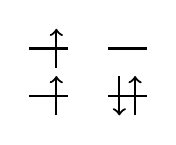
\begin{tikzpicture}[baseline={(current bounding box.center)}]
    % oberste MOs:
    \draw[thick] (0,0) -- (0.5,0); % erster Strich
    \draw[thick] (1,0) -- (1.5,0); % zweiter Strich
    % unterste MOs:
    \draw[thick] (0,-0.6) -- (0.5,-0.6); % dritter Strich
    \draw[thick] (1,-0.6) -- (1.5,-0.6); % vierter Strich
\draw[->, thick] (0.35, -0.25) -- (0.35, 0.25); 
\draw[-> , thick] (0.35, -0.85) -- (0.35, -0.35); 
 \draw[-> , thick] (1.35, -0.85) -- (1.35, -0.35); 
\draw[<- , thick] (1.15, -0.85) -- (1.15, -0.35); 
\end{tikzpicture}\right)\]$$+ \underbrace{(b_2^{*l})\cdot (b_2^{l})}_{\text{l: }a_1}\cdot \underbrace{(b_2^{*r})\cdot (a_2^{r})}_{\text{r: }b_1}\Rightarrow +\left|(b_2^{l}) \cdot (b_2^{*l}) \cdot (b_2^{*r}) \cdot (a_2^{r})\right|$$$$=+\left|(+a_{g}+b_u) \cdot (+a_g^{*}+b_u^{*}) \cdot (-a_g^{*}+b_u^{*}) \cdot (+a_{u}-b_g)\right|$$\begin{multline*}
=+\left|\underbrace{a_{g} a_g^{*} b_u^{*} a_{u}}_{b_g}\right|-\left|\underbrace{a_{g} a_g^{*} b_u^{*} b_g}_{a_{u}}\right|-\left|\underbrace{a_{g} b_u^{*} a_g^{*} a_{u}}_{b_g}\right|+\left|\underbrace{a_{g} b_u^{*} a_g^{*} b_g}_{a_{u}}\right|\\
+\left|\underbrace{b_u a_g^{*} b_u^{*} a_{u}}_{a_{u}}\right|-\left|\underbrace{b_u a_g^{*} b_u^{*} b_g}_{b_g}\right|-\left|\underbrace{b_u b_u^{*} a_g^{*} a_{u}}_{a_{u}}\right|+\left|\underbrace{b_u b_u^{*} a_g^{*} b_g}_{b_g}\right|\\
\end{multline*}\begin{multline*}
=+\left|\underbrace{a_{g} a_g^{*} b_u^{*} a_{u}}_{b_g}\right|+\left|\underbrace{a_{g} a_g^{*} b_g b_u^{*}}_{a_{u}}\right|+\left|\underbrace{a_{g} a_g^{*} b_u^{*} a_{u}}_{b_g}\right|+\left|\underbrace{a_{g} a_g^{*} b_g b_u^{*}}_{a_{u}}\right|\\
-\left|\underbrace{a_g^{*} b_u b_u^{*} a_{u}}_{a_{u}}\right|+\left|\underbrace{a_g^{*} b_g b_u b_u^{*}}_{b_g}\right|-\left|\underbrace{a_g^{*} b_u b_u^{*} a_{u}}_{a_{u}}\right|+\left|\underbrace{a_g^{*} b_g b_u b_u^{*}}_{b_g}\right|\\
\end{multline*}summarized:\begin{multline*}
=+2\left|\underbrace{a_{g} a_g^{*} b_u^{*} a_{u}}_{b_g}\right|+2\left|\underbrace{a_{g} a_g^{*} b_g b_u^{*}}_{a_{u}}\right|-2\left|\underbrace{a_g^{*} b_u b_u^{*} a_{u}}_{a_{u}}\right|+2\left|\underbrace{a_g^{*} b_g b_u b_u^{*}}_{b_g}\right|\\
\end{multline*}\\ \\
\hrule\newpage 


\[+\left(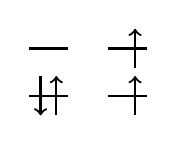
\begin{tikzpicture}[baseline={(current bounding box.center)}]
    % oberste MOs:
    \draw[thick] (0,0) -- (0.5,0); % erster Strich
    \draw[thick] (1,0) -- (1.5,0); % zweiter Strich
    % unterste MOs:
    \draw[thick] (0,-0.6) -- (0.5,-0.6); % dritter Strich
    \draw[thick] (1,-0.6) -- (1.5,-0.6); % vierter Strich
\draw[->, thick] (1.35, -0.25) -- (1.35, 0.25); 
\draw[-> , thick] (0.35, -0.85) -- (0.35, -0.35); 
\draw[<- , thick] (0.15, -0.85) -- (0.15, -0.35); 
 \draw[-> , thick] (1.35, -0.85) -- (1.35, -0.35); 
\end{tikzpicture}\qquad 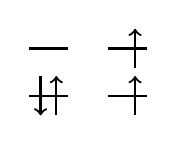
\begin{tikzpicture}[baseline={(current bounding box.center)}]
    % oberste MOs:
    \draw[thick] (0,0) -- (0.5,0); % erster Strich
    \draw[thick] (1,0) -- (1.5,0); % zweiter Strich
    % unterste MOs:
    \draw[thick] (0,-0.6) -- (0.5,-0.6); % dritter Strich
    \draw[thick] (1,-0.6) -- (1.5,-0.6); % vierter Strich
\draw[->, thick] (1.35, -0.25) -- (1.35, 0.25); 
\draw[-> , thick] (0.35, -0.85) -- (0.35, -0.35); 
\draw[<- , thick] (0.15, -0.85) -- (0.15, -0.35); 
 \draw[-> , thick] (1.35, -0.85) -- (1.35, -0.35); 
\end{tikzpicture}\right)\]$$+ \underbrace{(a_2^{*l})\cdot (b_2^{l})}_{\text{l: }b_1}\cdot \underbrace{(a_2^{*r})\cdot (b_2^{r})}_{\text{r: }b_1}\Rightarrow +\left|(b_2^{l}) \cdot (b_2^{r}) \cdot (a_2^{*l}) \cdot (a_2^{*r})\right|$$$$=+\left|(+a_{g}+b_u) \cdot (-a_{g}+b_u) \cdot (+a_u^{*}+b_g^{*}) \cdot (+a_u^{*}-b_g^{*})\right|$$\begin{multline*}
=-\left|\underbrace{a_{g} b_u a_u^{*} b_g^{*}}_{a_{g}}\right|+\left|\underbrace{a_{g} b_u b_g^{*} a_u^{*}}_{a_{g}}\right|+\left|\underbrace{b_u a_{g} a_u^{*} b_g^{*}}_{a_{g}}\right|-\left|\underbrace{b_u a_{g} b_g^{*} a_u^{*}}_{a_{g}}\right|\\
\end{multline*}\begin{multline*}
=-\left|\underbrace{a_{g} b_g^{*} b_u a_u^{*}}_{a_{g}}\right|-\left|\underbrace{a_{g} b_g^{*} b_u a_u^{*}}_{a_{g}}\right|-\left|\underbrace{a_{g} b_g^{*} b_u a_u^{*}}_{a_{g}}\right|-\left|\underbrace{a_{g} b_g^{*} b_u a_u^{*}}_{a_{g}}\right|\\
\end{multline*}summarized:\begin{multline*}
=-4\left|\underbrace{a_{g} b_g^{*} b_u a_u^{*}}_{a_{g}}\right|
\end{multline*}\\ \\
\hrule\newpage 


\[+\left(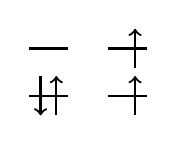
\begin{tikzpicture}[baseline={(current bounding box.center)}]
    % oberste MOs:
    \draw[thick] (0,0) -- (0.5,0); % erster Strich
    \draw[thick] (1,0) -- (1.5,0); % zweiter Strich
    % unterste MOs:
    \draw[thick] (0,-0.6) -- (0.5,-0.6); % dritter Strich
    \draw[thick] (1,-0.6) -- (1.5,-0.6); % vierter Strich
\draw[->, thick] (1.35, -0.25) -- (1.35, 0.25); 
\draw[-> , thick] (0.35, -0.85) -- (0.35, -0.35); 
\draw[<- , thick] (0.15, -0.85) -- (0.15, -0.35); 
 \draw[-> , thick] (1.35, -0.85) -- (1.35, -0.35); 
\end{tikzpicture}\qquad 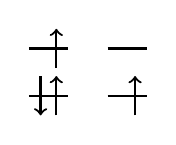
\begin{tikzpicture}[baseline={(current bounding box.center)}]
    % oberste MOs:
    \draw[thick] (0,0) -- (0.5,0); % erster Strich
    \draw[thick] (1,0) -- (1.5,0); % zweiter Strich
    % unterste MOs:
    \draw[thick] (0,-0.6) -- (0.5,-0.6); % dritter Strich
    \draw[thick] (1,-0.6) -- (1.5,-0.6); % vierter Strich
\draw[->, thick] (0.35, -0.25) -- (0.35, 0.25); 
\draw[-> , thick] (0.35, -0.85) -- (0.35, -0.35); 
\draw[<- , thick] (0.15, -0.85) -- (0.15, -0.35); 
 \draw[-> , thick] (1.35, -0.85) -- (1.35, -0.35); 
\end{tikzpicture}\right)\]$$+ \underbrace{(a_2^{*l})\cdot (b_2^{l})}_{\text{l: }b_1}\cdot \underbrace{(b_2^{*r})\cdot (b_2^{r})}_{\text{r: }a_1}\Rightarrow +\left|(b_2^{l}) \cdot (b_2^{r}) \cdot (b_2^{*r}) \cdot (a_2^{*l})\right|$$$$=+\left|(+a_{g}+b_u) \cdot (-a_{g}+b_u) \cdot (-a_g^{*}+b_u^{*}) \cdot (+a_u^{*}+b_g^{*})\right|$$\begin{multline*}
=-\left|\underbrace{a_{g} b_u a_g^{*} a_u^{*}}_{b_g}\right|-\left|\underbrace{a_{g} b_u a_g^{*} b_g^{*}}_{a_{u}}\right|+\left|\underbrace{a_{g} b_u b_u^{*} a_u^{*}}_{a_{u}}\right|+\left|\underbrace{a_{g} b_u b_u^{*} b_g^{*}}_{b_g}\right|\\
+\left|\underbrace{b_u a_{g} a_g^{*} a_u^{*}}_{b_g}\right|+\left|\underbrace{b_u a_{g} a_g^{*} b_g^{*}}_{a_{u}}\right|-\left|\underbrace{b_u a_{g} b_u^{*} a_u^{*}}_{a_{u}}\right|-\left|\underbrace{b_u a_{g} b_u^{*} b_g^{*}}_{b_g}\right|\\
\end{multline*}\begin{multline*}
=+\left|\underbrace{a_{g} a_g^{*} b_u a_u^{*}}_{b_g}\right|-\left|\underbrace{a_{g} a_g^{*} b_g^{*} b_u}_{a_{u}}\right|+\left|\underbrace{a_{g} b_u b_u^{*} a_u^{*}}_{a_{u}}\right|+\left|\underbrace{a_{g} b_g^{*} b_u b_u^{*}}_{b_g}\right|\\
+\left|\underbrace{a_{g} a_g^{*} b_u a_u^{*}}_{b_g}\right|-\left|\underbrace{a_{g} a_g^{*} b_g^{*} b_u}_{a_{u}}\right|+\left|\underbrace{a_{g} b_u b_u^{*} a_u^{*}}_{a_{u}}\right|+\left|\underbrace{a_{g} b_g^{*} b_u b_u^{*}}_{b_g}\right|\\
\end{multline*}summarized:\begin{multline*}
=+2\left|\underbrace{a_{g} a_g^{*} b_u a_u^{*}}_{b_g}\right|-2\left|\underbrace{a_{g} a_g^{*} b_g^{*} b_u}_{a_{u}}\right|+2\left|\underbrace{a_{g} b_u b_u^{*} a_u^{*}}_{a_{u}}\right|+2\left|\underbrace{a_{g} b_g^{*} b_u b_u^{*}}_{b_g}\right|\\
\end{multline*}\\ \\
\vspace{0.5cm}

\[+\left(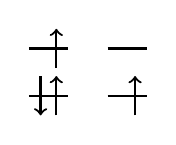
\begin{tikzpicture}[baseline={(current bounding box.center)}]
    % oberste MOs:
    \draw[thick] (0,0) -- (0.5,0); % erster Strich
    \draw[thick] (1,0) -- (1.5,0); % zweiter Strich
    % unterste MOs:
    \draw[thick] (0,-0.6) -- (0.5,-0.6); % dritter Strich
    \draw[thick] (1,-0.6) -- (1.5,-0.6); % vierter Strich
\draw[->, thick] (0.35, -0.25) -- (0.35, 0.25); 
\draw[-> , thick] (0.35, -0.85) -- (0.35, -0.35); 
\draw[<- , thick] (0.15, -0.85) -- (0.15, -0.35); 
 \draw[-> , thick] (1.35, -0.85) -- (1.35, -0.35); 
\end{tikzpicture}\qquad 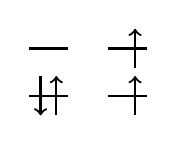
\begin{tikzpicture}[baseline={(current bounding box.center)}]
    % oberste MOs:
    \draw[thick] (0,0) -- (0.5,0); % erster Strich
    \draw[thick] (1,0) -- (1.5,0); % zweiter Strich
    % unterste MOs:
    \draw[thick] (0,-0.6) -- (0.5,-0.6); % dritter Strich
    \draw[thick] (1,-0.6) -- (1.5,-0.6); % vierter Strich
\draw[->, thick] (1.35, -0.25) -- (1.35, 0.25); 
\draw[-> , thick] (0.35, -0.85) -- (0.35, -0.35); 
\draw[<- , thick] (0.15, -0.85) -- (0.15, -0.35); 
 \draw[-> , thick] (1.35, -0.85) -- (1.35, -0.35); 
\end{tikzpicture}\right)\]$$+ \underbrace{(b_2^{*l})\cdot (b_2^{l})}_{\text{l: }a_1}\cdot \underbrace{(a_2^{*r})\cdot (b_2^{r})}_{\text{r: }b_1}\Rightarrow +\left|(b_2^{l}) \cdot (b_2^{r}) \cdot (b_2^{*l}) \cdot (a_2^{*r})\right|$$$$=+\left|(+a_{g}+b_u) \cdot (-a_{g}+b_u) \cdot (+a_g^{*}+b_u^{*}) \cdot (+a_u^{*}-b_g^{*})\right|$$\begin{multline*}
=+\left|\underbrace{a_{g} b_u a_g^{*} a_u^{*}}_{b_g}\right|-\left|\underbrace{a_{g} b_u a_g^{*} b_g^{*}}_{a_{u}}\right|+\left|\underbrace{a_{g} b_u b_u^{*} a_u^{*}}_{a_{u}}\right|-\left|\underbrace{a_{g} b_u b_u^{*} b_g^{*}}_{b_g}\right|\\
-\left|\underbrace{b_u a_{g} a_g^{*} a_u^{*}}_{b_g}\right|+\left|\underbrace{b_u a_{g} a_g^{*} b_g^{*}}_{a_{u}}\right|-\left|\underbrace{b_u a_{g} b_u^{*} a_u^{*}}_{a_{u}}\right|+\left|\underbrace{b_u a_{g} b_u^{*} b_g^{*}}_{b_g}\right|\\
\end{multline*}\begin{multline*}
=-\left|\underbrace{a_{g} a_g^{*} b_u a_u^{*}}_{b_g}\right|-\left|\underbrace{a_{g} a_g^{*} b_g^{*} b_u}_{a_{u}}\right|+\left|\underbrace{a_{g} b_u b_u^{*} a_u^{*}}_{a_{u}}\right|-\left|\underbrace{a_{g} b_g^{*} b_u b_u^{*}}_{b_g}\right|\\
-\left|\underbrace{a_{g} a_g^{*} b_u a_u^{*}}_{b_g}\right|-\left|\underbrace{a_{g} a_g^{*} b_g^{*} b_u}_{a_{u}}\right|+\left|\underbrace{a_{g} b_u b_u^{*} a_u^{*}}_{a_{u}}\right|-\left|\underbrace{a_{g} b_g^{*} b_u b_u^{*}}_{b_g}\right|\\
\end{multline*}summarized:\begin{multline*}
=-2\left|\underbrace{a_{g} a_g^{*} b_u a_u^{*}}_{b_g}\right|-2\left|\underbrace{a_{g} a_g^{*} b_g^{*} b_u}_{a_{u}}\right|+2\left|\underbrace{a_{g} b_u b_u^{*} a_u^{*}}_{a_{u}}\right|-2\left|\underbrace{a_{g} b_g^{*} b_u b_u^{*}}_{b_g}\right|\\
\end{multline*}\\ \\
\hrule\newpage 


\[+\left(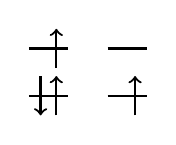
\begin{tikzpicture}[baseline={(current bounding box.center)}]
    % oberste MOs:
    \draw[thick] (0,0) -- (0.5,0); % erster Strich
    \draw[thick] (1,0) -- (1.5,0); % zweiter Strich
    % unterste MOs:
    \draw[thick] (0,-0.6) -- (0.5,-0.6); % dritter Strich
    \draw[thick] (1,-0.6) -- (1.5,-0.6); % vierter Strich
\draw[->, thick] (0.35, -0.25) -- (0.35, 0.25); 
\draw[-> , thick] (0.35, -0.85) -- (0.35, -0.35); 
\draw[<- , thick] (0.15, -0.85) -- (0.15, -0.35); 
 \draw[-> , thick] (1.35, -0.85) -- (1.35, -0.35); 
\end{tikzpicture}\qquad 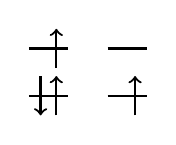
\begin{tikzpicture}[baseline={(current bounding box.center)}]
    % oberste MOs:
    \draw[thick] (0,0) -- (0.5,0); % erster Strich
    \draw[thick] (1,0) -- (1.5,0); % zweiter Strich
    % unterste MOs:
    \draw[thick] (0,-0.6) -- (0.5,-0.6); % dritter Strich
    \draw[thick] (1,-0.6) -- (1.5,-0.6); % vierter Strich
\draw[->, thick] (0.35, -0.25) -- (0.35, 0.25); 
\draw[-> , thick] (0.35, -0.85) -- (0.35, -0.35); 
\draw[<- , thick] (0.15, -0.85) -- (0.15, -0.35); 
 \draw[-> , thick] (1.35, -0.85) -- (1.35, -0.35); 
\end{tikzpicture}\right)\]$$+ \underbrace{(b_2^{*l})\cdot (b_2^{l})}_{\text{l: }a_1}\cdot \underbrace{(b_2^{*r})\cdot (b_2^{r})}_{\text{r: }a_1}\Rightarrow +\left|(b_2^{l}) \cdot (b_2^{r}) \cdot (b_2^{*l}) \cdot (b_2^{*r})\right|$$$$=+\left|(+a_{g}+b_u) \cdot (-a_{g}+b_u) \cdot (+a_g^{*}+b_u^{*}) \cdot (-a_g^{*}+b_u^{*})\right|$$\begin{multline*}
=+\left|\underbrace{a_{g} b_u a_g^{*} b_u^{*}}_{a_{g}}\right|-\left|\underbrace{a_{g} b_u b_u^{*} a_g^{*}}_{a_{g}}\right|-\left|\underbrace{b_u a_{g} a_g^{*} b_u^{*}}_{a_{g}}\right|+\left|\underbrace{b_u a_{g} b_u^{*} a_g^{*}}_{a_{g}}\right|\\
\end{multline*}\begin{multline*}
=-\left|\underbrace{a_{g} a_g^{*} b_u b_u^{*}}_{a_{g}}\right|-\left|\underbrace{a_{g} a_g^{*} b_u b_u^{*}}_{a_{g}}\right|-\left|\underbrace{a_{g} a_g^{*} b_u b_u^{*}}_{a_{g}}\right|-\left|\underbrace{a_{g} a_g^{*} b_u b_u^{*}}_{a_{g}}\right|\\
\end{multline*}summarized:\begin{multline*}
=-4\left|\underbrace{a_{g} a_g^{*} b_u b_u^{*}}_{a_{g}}\right|
\end{multline*}\\ \\
\hrule\newpage 

\newpage \section{Linear Combinations: 4 Monomer- / 2 Dimer-States}
\[ +\left(\text{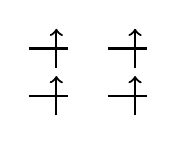
\begin{tikzpicture}[baseline={(current bounding box.center)}]
    % oberste MOs:
    \draw[thick] (0,0) -- (0.5,0); % erster Strich
    \draw[thick] (1,0) -- (1.5,0); % zweiter Strich
    % unterste MOs:
    \draw[thick] (0,-0.6) -- (0.5,-0.6); % dritter Strich
    \draw[thick] (1,-0.6) -- (1.5,-0.6); % vierter Strich
\draw[->, thick] (0.35, -0.25) -- (0.35, 0.25); 
\draw[->, thick] (1.35, -0.25) -- (1.35, 0.25); 
\draw[-> , thick] (0.35, -0.85) -- (0.35, -0.35); 
 \draw[-> , thick] (1.35, -0.85) -- (1.35, -0.35); 
\end{tikzpicture}\qquad 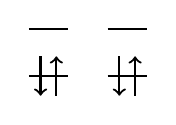
\begin{tikzpicture}[baseline={(current bounding box.center)}]
    % oberste MOs:
    \draw[thick] (0,0) -- (0.5,0); % erster Strich
    \draw[thick] (1,0) -- (1.5,0); % zweiter Strich
    % unterste MOs:
    \draw[thick] (0,-0.6) -- (0.5,-0.6); % dritter Strich
    \draw[thick] (1,-0.6) -- (1.5,-0.6); % vierter Strich
\draw[-> , thick] (0.35, -0.85) -- (0.35, -0.35); 
\draw[<- , thick] (0.15, -0.85) -- (0.15, -0.35); 
 \draw[-> , thick] (1.35, -0.85) -- (1.35, -0.35); 
\draw[<- , thick] (1.15, -0.85) -- (1.15, -0.35); 
\end{tikzpicture}}\right)+\left(\text{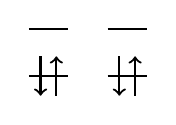
\begin{tikzpicture}[baseline={(current bounding box.center)}]
    % oberste MOs:
    \draw[thick] (0,0) -- (0.5,0); % erster Strich
    \draw[thick] (1,0) -- (1.5,0); % zweiter Strich
    % unterste MOs:
    \draw[thick] (0,-0.6) -- (0.5,-0.6); % dritter Strich
    \draw[thick] (1,-0.6) -- (1.5,-0.6); % vierter Strich
\draw[-> , thick] (0.35, -0.85) -- (0.35, -0.35); 
\draw[<- , thick] (0.15, -0.85) -- (0.15, -0.35); 
 \draw[-> , thick] (1.35, -0.85) -- (1.35, -0.35); 
\draw[<- , thick] (1.15, -0.85) -- (1.15, -0.35); 
\end{tikzpicture}\qquad 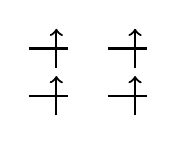
\begin{tikzpicture}[baseline={(current bounding box.center)}]
    % oberste MOs:
    \draw[thick] (0,0) -- (0.5,0); % erster Strich
    \draw[thick] (1,0) -- (1.5,0); % zweiter Strich
    % unterste MOs:
    \draw[thick] (0,-0.6) -- (0.5,-0.6); % dritter Strich
    \draw[thick] (1,-0.6) -- (1.5,-0.6); % vierter Strich
\draw[->, thick] (0.35, -0.25) -- (0.35, 0.25); 
\draw[->, thick] (1.35, -0.25) -- (1.35, 0.25); 
\draw[-> , thick] (0.35, -0.85) -- (0.35, -0.35); 
 \draw[-> , thick] (1.35, -0.85) -- (1.35, -0.35); 
\end{tikzpicture}}\right)\]enthaltene Monomer-Symmetrien = $a_{g},a_1$\begin{multline*}=+\left(\left|(b_2^{l}) \cdot (b_2^{*l}) \cdot (a_2^{l}) \cdot (a_2^{*l})\right|\right)+\left(\left|(b_2^{r}) \cdot (b_2^{*r}) \cdot (a_2^{r}) \cdot (a_2^{*r})\right|\right)\end{multline*}
\begin{multline*}
=+2\left|\underbrace{a_{g} a_g^{*} a_{u} a_u^{*}}_{a_{g}}\right|+2\left|\underbrace{a_{g} a_g^{*} b_g b_g^{*}}_{a_{g}}\right|+2\left|\underbrace{a_{g} b_g^{*} b_u^{*} a_{u}}_{a_{g}}\right|-2\left|\underbrace{a_{g} b_g b_u^{*} a_u^{*}}_{a_{g}}\right|\\
-2\left|\underbrace{a_g^{*} b_g^{*} b_u a_{u}}_{a_{g}}\right|+2\left|\underbrace{a_g^{*} b_g b_u a_u^{*}}_{a_{g}}\right|+2\left|\underbrace{b_u b_u^{*} a_{u} a_u^{*}}_{a_{g}}\right|+2\left|\underbrace{b_g b_g^{*} b_u b_u^{*}}_{a_{g}}\right|
\end{multline*}
\\\\


\vspace{0.5cm}
\[ +\left(\text{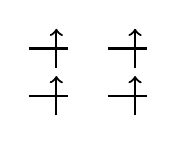
\begin{tikzpicture}[baseline={(current bounding box.center)}]
    % oberste MOs:
    \draw[thick] (0,0) -- (0.5,0); % erster Strich
    \draw[thick] (1,0) -- (1.5,0); % zweiter Strich
    % unterste MOs:
    \draw[thick] (0,-0.6) -- (0.5,-0.6); % dritter Strich
    \draw[thick] (1,-0.6) -- (1.5,-0.6); % vierter Strich
\draw[->, thick] (0.35, -0.25) -- (0.35, 0.25); 
\draw[->, thick] (1.35, -0.25) -- (1.35, 0.25); 
\draw[-> , thick] (0.35, -0.85) -- (0.35, -0.35); 
 \draw[-> , thick] (1.35, -0.85) -- (1.35, -0.35); 
\end{tikzpicture}\qquad 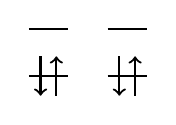
\begin{tikzpicture}[baseline={(current bounding box.center)}]
    % oberste MOs:
    \draw[thick] (0,0) -- (0.5,0); % erster Strich
    \draw[thick] (1,0) -- (1.5,0); % zweiter Strich
    % unterste MOs:
    \draw[thick] (0,-0.6) -- (0.5,-0.6); % dritter Strich
    \draw[thick] (1,-0.6) -- (1.5,-0.6); % vierter Strich
\draw[-> , thick] (0.35, -0.85) -- (0.35, -0.35); 
\draw[<- , thick] (0.15, -0.85) -- (0.15, -0.35); 
 \draw[-> , thick] (1.35, -0.85) -- (1.35, -0.35); 
\draw[<- , thick] (1.15, -0.85) -- (1.15, -0.35); 
\end{tikzpicture}}\right)-\left(\text{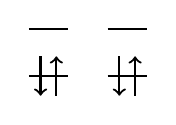
\begin{tikzpicture}[baseline={(current bounding box.center)}]
    % oberste MOs:
    \draw[thick] (0,0) -- (0.5,0); % erster Strich
    \draw[thick] (1,0) -- (1.5,0); % zweiter Strich
    % unterste MOs:
    \draw[thick] (0,-0.6) -- (0.5,-0.6); % dritter Strich
    \draw[thick] (1,-0.6) -- (1.5,-0.6); % vierter Strich
\draw[-> , thick] (0.35, -0.85) -- (0.35, -0.35); 
\draw[<- , thick] (0.15, -0.85) -- (0.15, -0.35); 
 \draw[-> , thick] (1.35, -0.85) -- (1.35, -0.35); 
\draw[<- , thick] (1.15, -0.85) -- (1.15, -0.35); 
\end{tikzpicture}\qquad 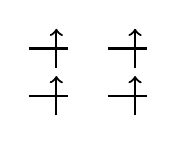
\begin{tikzpicture}[baseline={(current bounding box.center)}]
    % oberste MOs:
    \draw[thick] (0,0) -- (0.5,0); % erster Strich
    \draw[thick] (1,0) -- (1.5,0); % zweiter Strich
    % unterste MOs:
    \draw[thick] (0,-0.6) -- (0.5,-0.6); % dritter Strich
    \draw[thick] (1,-0.6) -- (1.5,-0.6); % vierter Strich
\draw[->, thick] (0.35, -0.25) -- (0.35, 0.25); 
\draw[->, thick] (1.35, -0.25) -- (1.35, 0.25); 
\draw[-> , thick] (0.35, -0.85) -- (0.35, -0.35); 
 \draw[-> , thick] (1.35, -0.85) -- (1.35, -0.35); 
\end{tikzpicture}}\right)\]enthaltene Monomer-Symmetrien = $a_{g},a_1$\begin{multline*}=+\left(\left|(b_2^{l}) \cdot (b_2^{*l}) \cdot (a_2^{l}) \cdot (a_2^{*l})\right|\right)-\left(\left|(b_2^{r}) \cdot (b_2^{*r}) \cdot (a_2^{r}) \cdot (a_2^{*r})\right|\right)\end{multline*}
\begin{multline*}
=-2\left|\underbrace{a_{g} a_g^{*} b_g^{*} a_{u}}_{b_u}\right|+2\left|\underbrace{a_{g} a_g^{*} b_g a_u^{*}}_{b_u}\right|+2\left|\underbrace{a_{g} b_u^{*} a_{u} a_u^{*}}_{b_u}\right|+2\left|\underbrace{a_{g} b_g b_g^{*} b_u^{*}}_{b_u}\right|\\
-2\left|\underbrace{a_g^{*} b_u a_{u} a_u^{*}}_{b_u}\right|-2\left|\underbrace{a_g^{*} b_g b_g^{*} b_u}_{b_u}\right|-2\left|\underbrace{b_g^{*} b_u b_u^{*} a_{u}}_{b_u}\right|+2\left|\underbrace{b_g b_u b_u^{*} a_u^{*}}_{b_u}\right|
\end{multline*}
\\\\


\hrule\newpage 
\[ +\left(\text{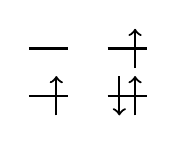
\begin{tikzpicture}[baseline={(current bounding box.center)}]
    % oberste MOs:
    \draw[thick] (0,0) -- (0.5,0); % erster Strich
    \draw[thick] (1,0) -- (1.5,0); % zweiter Strich
    % unterste MOs:
    \draw[thick] (0,-0.6) -- (0.5,-0.6); % dritter Strich
    \draw[thick] (1,-0.6) -- (1.5,-0.6); % vierter Strich
\draw[->, thick] (1.35, -0.25) -- (1.35, 0.25); 
\draw[-> , thick] (0.35, -0.85) -- (0.35, -0.35); 
 \draw[-> , thick] (1.35, -0.85) -- (1.35, -0.35); 
\draw[<- , thick] (1.15, -0.85) -- (1.15, -0.35); 
\end{tikzpicture}\qquad 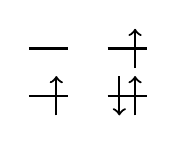
\begin{tikzpicture}[baseline={(current bounding box.center)}]
    % oberste MOs:
    \draw[thick] (0,0) -- (0.5,0); % erster Strich
    \draw[thick] (1,0) -- (1.5,0); % zweiter Strich
    % unterste MOs:
    \draw[thick] (0,-0.6) -- (0.5,-0.6); % dritter Strich
    \draw[thick] (1,-0.6) -- (1.5,-0.6); % vierter Strich
\draw[->, thick] (1.35, -0.25) -- (1.35, 0.25); 
\draw[-> , thick] (0.35, -0.85) -- (0.35, -0.35); 
 \draw[-> , thick] (1.35, -0.85) -- (1.35, -0.35); 
\draw[<- , thick] (1.15, -0.85) -- (1.15, -0.35); 
\end{tikzpicture}}\right)+\left(\text{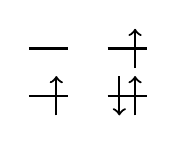
\begin{tikzpicture}[baseline={(current bounding box.center)}]
    % oberste MOs:
    \draw[thick] (0,0) -- (0.5,0); % erster Strich
    \draw[thick] (1,0) -- (1.5,0); % zweiter Strich
    % unterste MOs:
    \draw[thick] (0,-0.6) -- (0.5,-0.6); % dritter Strich
    \draw[thick] (1,-0.6) -- (1.5,-0.6); % vierter Strich
\draw[->, thick] (1.35, -0.25) -- (1.35, 0.25); 
\draw[-> , thick] (0.35, -0.85) -- (0.35, -0.35); 
 \draw[-> , thick] (1.35, -0.85) -- (1.35, -0.35); 
\draw[<- , thick] (1.15, -0.85) -- (1.15, -0.35); 
\end{tikzpicture}\qquad 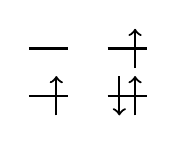
\begin{tikzpicture}[baseline={(current bounding box.center)}]
    % oberste MOs:
    \draw[thick] (0,0) -- (0.5,0); % erster Strich
    \draw[thick] (1,0) -- (1.5,0); % zweiter Strich
    % unterste MOs:
    \draw[thick] (0,-0.6) -- (0.5,-0.6); % dritter Strich
    \draw[thick] (1,-0.6) -- (1.5,-0.6); % vierter Strich
\draw[->, thick] (1.35, -0.25) -- (1.35, 0.25); 
\draw[-> , thick] (0.35, -0.85) -- (0.35, -0.35); 
 \draw[-> , thick] (1.35, -0.85) -- (1.35, -0.35); 
\draw[<- , thick] (1.15, -0.85) -- (1.15, -0.35); 
\end{tikzpicture}}\right)\]enthaltene Monomer-Symmetrien = $a_1$\begin{multline*}=+\left(\left|(a_2^{l}) \cdot (a_2^{r}) \cdot (a_2^{*l}) \cdot (a_2^{*r})\right|\right)+\left(\left|(a_2^{l}) \cdot (a_2^{r}) \cdot (a_2^{*l}) \cdot (a_2^{*r})\right|\right)\end{multline*}
\begin{multline*}
=-8\left|\underbrace{b_g b_g^{*} a_{u} a_u^{*}}_{a_{g}}\right|
\end{multline*}
\\\\


\hrule\newpage 
\[ +\left(\text{\begin{tikzpicture}[baseline={(current bounding box.center)}]
    % oberste MOs:
    \draw[thick] (0,0) -- (0.5,0); % erster Strich
    \draw[thick] (1,0) -- (1.5,0); % zweiter Strich
    % unterste MOs:
    \draw[thick] (0,-0.6) -- (0.5,-0.6); % dritter Strich
    \draw[thick] (1,-0.6) -- (1.5,-0.6); % vierter Strich
\draw[->, thick] (1.35, -0.25) -- (1.35, 0.25); 
\draw[-> , thick] (0.35, -0.85) -- (0.35, -0.35); 
 \draw[-> , thick] (1.35, -0.85) -- (1.35, -0.35); 
\draw[<- , thick] (1.15, -0.85) -- (1.15, -0.35); 
\end{tikzpicture}\qquad \begin{tikzpicture}[baseline={(current bounding box.center)}]
    % oberste MOs:
    \draw[thick] (0,0) -- (0.5,0); % erster Strich
    \draw[thick] (1,0) -- (1.5,0); % zweiter Strich
    % unterste MOs:
    \draw[thick] (0,-0.6) -- (0.5,-0.6); % dritter Strich
    \draw[thick] (1,-0.6) -- (1.5,-0.6); % vierter Strich
\draw[->, thick] (0.35, -0.25) -- (0.35, 0.25); 
\draw[-> , thick] (0.35, -0.85) -- (0.35, -0.35); 
 \draw[-> , thick] (1.35, -0.85) -- (1.35, -0.35); 
\draw[<- , thick] (1.15, -0.85) -- (1.15, -0.35); 
\end{tikzpicture}}\right)+\left(\text{\begin{tikzpicture}[baseline={(current bounding box.center)}]
    % oberste MOs:
    \draw[thick] (0,0) -- (0.5,0); % erster Strich
    \draw[thick] (1,0) -- (1.5,0); % zweiter Strich
    % unterste MOs:
    \draw[thick] (0,-0.6) -- (0.5,-0.6); % dritter Strich
    \draw[thick] (1,-0.6) -- (1.5,-0.6); % vierter Strich
\draw[->, thick] (0.35, -0.25) -- (0.35, 0.25); 
\draw[-> , thick] (0.35, -0.85) -- (0.35, -0.35); 
 \draw[-> , thick] (1.35, -0.85) -- (1.35, -0.35); 
\draw[<- , thick] (1.15, -0.85) -- (1.15, -0.35); 
\end{tikzpicture}\qquad \begin{tikzpicture}[baseline={(current bounding box.center)}]
    % oberste MOs:
    \draw[thick] (0,0) -- (0.5,0); % erster Strich
    \draw[thick] (1,0) -- (1.5,0); % zweiter Strich
    % unterste MOs:
    \draw[thick] (0,-0.6) -- (0.5,-0.6); % dritter Strich
    \draw[thick] (1,-0.6) -- (1.5,-0.6); % vierter Strich
\draw[->, thick] (1.35, -0.25) -- (1.35, 0.25); 
\draw[-> , thick] (0.35, -0.85) -- (0.35, -0.35); 
 \draw[-> , thick] (1.35, -0.85) -- (1.35, -0.35); 
\draw[<- , thick] (1.15, -0.85) -- (1.15, -0.35); 
\end{tikzpicture}}\right)\]enthaltene Monomer-Symmetrien = $b_1,a_1$\begin{multline*}=+\left(\left|(b_2^{*r}) \cdot (a_2^{l}) \cdot (a_2^{r}) \cdot (a_2^{*l})\right|\right)+\left(\left|(b_2^{*l}) \cdot (a_2^{l}) \cdot (a_2^{r}) \cdot (a_2^{*r})\right|\right)\end{multline*}
\begin{multline*}
=+4\left|\underbrace{a_g^{*} b_g b_g^{*} a_{u}}_{a_{u}}\right|-4\left|\underbrace{b_g b_u^{*} a_{u} a_u^{*}}_{a_{u}}\right|
\end{multline*}
\\\\


\vspace{0.5cm}
\[ +\left(\text{\begin{tikzpicture}[baseline={(current bounding box.center)}]
    % oberste MOs:
    \draw[thick] (0,0) -- (0.5,0); % erster Strich
    \draw[thick] (1,0) -- (1.5,0); % zweiter Strich
    % unterste MOs:
    \draw[thick] (0,-0.6) -- (0.5,-0.6); % dritter Strich
    \draw[thick] (1,-0.6) -- (1.5,-0.6); % vierter Strich
\draw[->, thick] (1.35, -0.25) -- (1.35, 0.25); 
\draw[-> , thick] (0.35, -0.85) -- (0.35, -0.35); 
 \draw[-> , thick] (1.35, -0.85) -- (1.35, -0.35); 
\draw[<- , thick] (1.15, -0.85) -- (1.15, -0.35); 
\end{tikzpicture}\qquad \begin{tikzpicture}[baseline={(current bounding box.center)}]
    % oberste MOs:
    \draw[thick] (0,0) -- (0.5,0); % erster Strich
    \draw[thick] (1,0) -- (1.5,0); % zweiter Strich
    % unterste MOs:
    \draw[thick] (0,-0.6) -- (0.5,-0.6); % dritter Strich
    \draw[thick] (1,-0.6) -- (1.5,-0.6); % vierter Strich
\draw[->, thick] (0.35, -0.25) -- (0.35, 0.25); 
\draw[-> , thick] (0.35, -0.85) -- (0.35, -0.35); 
 \draw[-> , thick] (1.35, -0.85) -- (1.35, -0.35); 
\draw[<- , thick] (1.15, -0.85) -- (1.15, -0.35); 
\end{tikzpicture}}\right)-\left(\text{\begin{tikzpicture}[baseline={(current bounding box.center)}]
    % oberste MOs:
    \draw[thick] (0,0) -- (0.5,0); % erster Strich
    \draw[thick] (1,0) -- (1.5,0); % zweiter Strich
    % unterste MOs:
    \draw[thick] (0,-0.6) -- (0.5,-0.6); % dritter Strich
    \draw[thick] (1,-0.6) -- (1.5,-0.6); % vierter Strich
\draw[->, thick] (0.35, -0.25) -- (0.35, 0.25); 
\draw[-> , thick] (0.35, -0.85) -- (0.35, -0.35); 
 \draw[-> , thick] (1.35, -0.85) -- (1.35, -0.35); 
\draw[<- , thick] (1.15, -0.85) -- (1.15, -0.35); 
\end{tikzpicture}\qquad \begin{tikzpicture}[baseline={(current bounding box.center)}]
    % oberste MOs:
    \draw[thick] (0,0) -- (0.5,0); % erster Strich
    \draw[thick] (1,0) -- (1.5,0); % zweiter Strich
    % unterste MOs:
    \draw[thick] (0,-0.6) -- (0.5,-0.6); % dritter Strich
    \draw[thick] (1,-0.6) -- (1.5,-0.6); % vierter Strich
\draw[->, thick] (1.35, -0.25) -- (1.35, 0.25); 
\draw[-> , thick] (0.35, -0.85) -- (0.35, -0.35); 
 \draw[-> , thick] (1.35, -0.85) -- (1.35, -0.35); 
\draw[<- , thick] (1.15, -0.85) -- (1.15, -0.35); 
\end{tikzpicture}}\right)\]enthaltene Monomer-Symmetrien = $b_1,a_1$\begin{multline*}=+\left(\left|(b_2^{*r}) \cdot (a_2^{l}) \cdot (a_2^{r}) \cdot (a_2^{*l})\right|\right)-\left(\left|(b_2^{*l}) \cdot (a_2^{l}) \cdot (a_2^{r}) \cdot (a_2^{*r})\right|\right)\end{multline*}
\begin{multline*}
=-4\left|\underbrace{a_g^{*} b_g a_{u} a_u^{*}}_{b_g}\right|-4\left|\underbrace{b_g b_g^{*} b_u^{*} a_{u}}_{b_g}\right|
\end{multline*}
\\\\


\hrule\newpage 
\[ +\left(\text{\begin{tikzpicture}[baseline={(current bounding box.center)}]
    % oberste MOs:
    \draw[thick] (0,0) -- (0.5,0); % erster Strich
    \draw[thick] (1,0) -- (1.5,0); % zweiter Strich
    % unterste MOs:
    \draw[thick] (0,-0.6) -- (0.5,-0.6); % dritter Strich
    \draw[thick] (1,-0.6) -- (1.5,-0.6); % vierter Strich
\draw[->, thick] (1.35, -0.25) -- (1.35, 0.25); 
\draw[-> , thick] (0.35, -0.85) -- (0.35, -0.35); 
 \draw[-> , thick] (1.35, -0.85) -- (1.35, -0.35); 
\draw[<- , thick] (1.15, -0.85) -- (1.15, -0.35); 
\end{tikzpicture}\qquad \begin{tikzpicture}[baseline={(current bounding box.center)}]
    % oberste MOs:
    \draw[thick] (0,0) -- (0.5,0); % erster Strich
    \draw[thick] (1,0) -- (1.5,0); % zweiter Strich
    % unterste MOs:
    \draw[thick] (0,-0.6) -- (0.5,-0.6); % dritter Strich
    \draw[thick] (1,-0.6) -- (1.5,-0.6); % vierter Strich
\draw[->, thick] (1.35, -0.25) -- (1.35, 0.25); 
\draw[-> , thick] (0.35, -0.85) -- (0.35, -0.35); 
\draw[<- , thick] (0.15, -0.85) -- (0.15, -0.35); 
 \draw[-> , thick] (1.35, -0.85) -- (1.35, -0.35); 
\end{tikzpicture}}\right)+\left(\text{\begin{tikzpicture}[baseline={(current bounding box.center)}]
    % oberste MOs:
    \draw[thick] (0,0) -- (0.5,0); % erster Strich
    \draw[thick] (1,0) -- (1.5,0); % zweiter Strich
    % unterste MOs:
    \draw[thick] (0,-0.6) -- (0.5,-0.6); % dritter Strich
    \draw[thick] (1,-0.6) -- (1.5,-0.6); % vierter Strich
\draw[->, thick] (1.35, -0.25) -- (1.35, 0.25); 
\draw[-> , thick] (0.35, -0.85) -- (0.35, -0.35); 
\draw[<- , thick] (0.15, -0.85) -- (0.15, -0.35); 
 \draw[-> , thick] (1.35, -0.85) -- (1.35, -0.35); 
\end{tikzpicture}\qquad \begin{tikzpicture}[baseline={(current bounding box.center)}]
    % oberste MOs:
    \draw[thick] (0,0) -- (0.5,0); % erster Strich
    \draw[thick] (1,0) -- (1.5,0); % zweiter Strich
    % unterste MOs:
    \draw[thick] (0,-0.6) -- (0.5,-0.6); % dritter Strich
    \draw[thick] (1,-0.6) -- (1.5,-0.6); % vierter Strich
\draw[->, thick] (1.35, -0.25) -- (1.35, 0.25); 
\draw[-> , thick] (0.35, -0.85) -- (0.35, -0.35); 
 \draw[-> , thick] (1.35, -0.85) -- (1.35, -0.35); 
\draw[<- , thick] (1.15, -0.85) -- (1.15, -0.35); 
\end{tikzpicture}}\right)\]enthaltene Monomer-Symmetrien = $b_1,a_1$\begin{multline*}=+\left(\left|(b_2^{r}) \cdot (a_2^{l}) \cdot (a_2^{*l}) \cdot (a_2^{*r})\right|\right)+\left(\left|(b_2^{l}) \cdot (a_2^{r}) \cdot (a_2^{*l}) \cdot (a_2^{*r})\right|\right)\end{multline*}
\begin{multline*}
=-4\left|\underbrace{a_{g} b_g b_g^{*} a_u^{*}}_{a_{u}}\right|+4\left|\underbrace{b_g^{*} b_u a_{u} a_u^{*}}_{a_{u}}\right|
\end{multline*}
\\\\


\vspace{0.5cm}
\[ +\left(\text{\begin{tikzpicture}[baseline={(current bounding box.center)}]
    % oberste MOs:
    \draw[thick] (0,0) -- (0.5,0); % erster Strich
    \draw[thick] (1,0) -- (1.5,0); % zweiter Strich
    % unterste MOs:
    \draw[thick] (0,-0.6) -- (0.5,-0.6); % dritter Strich
    \draw[thick] (1,-0.6) -- (1.5,-0.6); % vierter Strich
\draw[->, thick] (1.35, -0.25) -- (1.35, 0.25); 
\draw[-> , thick] (0.35, -0.85) -- (0.35, -0.35); 
 \draw[-> , thick] (1.35, -0.85) -- (1.35, -0.35); 
\draw[<- , thick] (1.15, -0.85) -- (1.15, -0.35); 
\end{tikzpicture}\qquad \begin{tikzpicture}[baseline={(current bounding box.center)}]
    % oberste MOs:
    \draw[thick] (0,0) -- (0.5,0); % erster Strich
    \draw[thick] (1,0) -- (1.5,0); % zweiter Strich
    % unterste MOs:
    \draw[thick] (0,-0.6) -- (0.5,-0.6); % dritter Strich
    \draw[thick] (1,-0.6) -- (1.5,-0.6); % vierter Strich
\draw[->, thick] (1.35, -0.25) -- (1.35, 0.25); 
\draw[-> , thick] (0.35, -0.85) -- (0.35, -0.35); 
\draw[<- , thick] (0.15, -0.85) -- (0.15, -0.35); 
 \draw[-> , thick] (1.35, -0.85) -- (1.35, -0.35); 
\end{tikzpicture}}\right)-\left(\text{\begin{tikzpicture}[baseline={(current bounding box.center)}]
    % oberste MOs:
    \draw[thick] (0,0) -- (0.5,0); % erster Strich
    \draw[thick] (1,0) -- (1.5,0); % zweiter Strich
    % unterste MOs:
    \draw[thick] (0,-0.6) -- (0.5,-0.6); % dritter Strich
    \draw[thick] (1,-0.6) -- (1.5,-0.6); % vierter Strich
\draw[->, thick] (1.35, -0.25) -- (1.35, 0.25); 
\draw[-> , thick] (0.35, -0.85) -- (0.35, -0.35); 
\draw[<- , thick] (0.15, -0.85) -- (0.15, -0.35); 
 \draw[-> , thick] (1.35, -0.85) -- (1.35, -0.35); 
\end{tikzpicture}\qquad \begin{tikzpicture}[baseline={(current bounding box.center)}]
    % oberste MOs:
    \draw[thick] (0,0) -- (0.5,0); % erster Strich
    \draw[thick] (1,0) -- (1.5,0); % zweiter Strich
    % unterste MOs:
    \draw[thick] (0,-0.6) -- (0.5,-0.6); % dritter Strich
    \draw[thick] (1,-0.6) -- (1.5,-0.6); % vierter Strich
\draw[->, thick] (1.35, -0.25) -- (1.35, 0.25); 
\draw[-> , thick] (0.35, -0.85) -- (0.35, -0.35); 
 \draw[-> , thick] (1.35, -0.85) -- (1.35, -0.35); 
\draw[<- , thick] (1.15, -0.85) -- (1.15, -0.35); 
\end{tikzpicture}}\right)\]enthaltene Monomer-Symmetrien = $b_1,a_1$\begin{multline*}=+\left(\left|(b_2^{r}) \cdot (a_2^{l}) \cdot (a_2^{*l}) \cdot (a_2^{*r})\right|\right)-\left(\left|(b_2^{l}) \cdot (a_2^{r}) \cdot (a_2^{*l}) \cdot (a_2^{*r})\right|\right)\end{multline*}
\begin{multline*}
=+4\left|\underbrace{a_{g} b_g^{*} a_{u} a_u^{*}}_{b_g}\right|+4\left|\underbrace{b_g b_g^{*} b_u a_u^{*}}_{b_g}\right|
\end{multline*}
\\\\


\hrule\newpage 
\[ +\left(\text{\begin{tikzpicture}[baseline={(current bounding box.center)}]
    % oberste MOs:
    \draw[thick] (0,0) -- (0.5,0); % erster Strich
    \draw[thick] (1,0) -- (1.5,0); % zweiter Strich
    % unterste MOs:
    \draw[thick] (0,-0.6) -- (0.5,-0.6); % dritter Strich
    \draw[thick] (1,-0.6) -- (1.5,-0.6); % vierter Strich
\draw[->, thick] (1.35, -0.25) -- (1.35, 0.25); 
\draw[-> , thick] (0.35, -0.85) -- (0.35, -0.35); 
 \draw[-> , thick] (1.35, -0.85) -- (1.35, -0.35); 
\draw[<- , thick] (1.15, -0.85) -- (1.15, -0.35); 
\end{tikzpicture}\qquad \begin{tikzpicture}[baseline={(current bounding box.center)}]
    % oberste MOs:
    \draw[thick] (0,0) -- (0.5,0); % erster Strich
    \draw[thick] (1,0) -- (1.5,0); % zweiter Strich
    % unterste MOs:
    \draw[thick] (0,-0.6) -- (0.5,-0.6); % dritter Strich
    \draw[thick] (1,-0.6) -- (1.5,-0.6); % vierter Strich
\draw[->, thick] (0.35, -0.25) -- (0.35, 0.25); 
\draw[-> , thick] (0.35, -0.85) -- (0.35, -0.35); 
\draw[<- , thick] (0.15, -0.85) -- (0.15, -0.35); 
 \draw[-> , thick] (1.35, -0.85) -- (1.35, -0.35); 
\end{tikzpicture}}\right)+\left(\text{\begin{tikzpicture}[baseline={(current bounding box.center)}]
    % oberste MOs:
    \draw[thick] (0,0) -- (0.5,0); % erster Strich
    \draw[thick] (1,0) -- (1.5,0); % zweiter Strich
    % unterste MOs:
    \draw[thick] (0,-0.6) -- (0.5,-0.6); % dritter Strich
    \draw[thick] (1,-0.6) -- (1.5,-0.6); % vierter Strich
\draw[->, thick] (0.35, -0.25) -- (0.35, 0.25); 
\draw[-> , thick] (0.35, -0.85) -- (0.35, -0.35); 
\draw[<- , thick] (0.15, -0.85) -- (0.15, -0.35); 
 \draw[-> , thick] (1.35, -0.85) -- (1.35, -0.35); 
\end{tikzpicture}\qquad \begin{tikzpicture}[baseline={(current bounding box.center)}]
    % oberste MOs:
    \draw[thick] (0,0) -- (0.5,0); % erster Strich
    \draw[thick] (1,0) -- (1.5,0); % zweiter Strich
    % unterste MOs:
    \draw[thick] (0,-0.6) -- (0.5,-0.6); % dritter Strich
    \draw[thick] (1,-0.6) -- (1.5,-0.6); % vierter Strich
\draw[->, thick] (1.35, -0.25) -- (1.35, 0.25); 
\draw[-> , thick] (0.35, -0.85) -- (0.35, -0.35); 
 \draw[-> , thick] (1.35, -0.85) -- (1.35, -0.35); 
\draw[<- , thick] (1.15, -0.85) -- (1.15, -0.35); 
\end{tikzpicture}}\right)\]enthaltene Monomer-Symmetrien = $a_1$\begin{multline*}=+\left(\left|(b_2^{r}) \cdot (b_2^{*r}) \cdot (a_2^{l}) \cdot (a_2^{*l})\right|\right)+\left(\left|(b_2^{l}) \cdot (b_2^{*l}) \cdot (a_2^{r}) \cdot (a_2^{*r})\right|\right)\end{multline*}
\begin{multline*}
=+2\left|\underbrace{a_{g} a_g^{*} a_{u} a_u^{*}}_{a_{g}}\right|+2\left|\underbrace{a_{g} a_g^{*} b_g b_g^{*}}_{a_{g}}\right|-2\left|\underbrace{a_{g} b_g^{*} b_u^{*} a_{u}}_{a_{g}}\right|+2\left|\underbrace{a_{g} b_g b_u^{*} a_u^{*}}_{a_{g}}\right|\\
+2\left|\underbrace{a_g^{*} b_g^{*} b_u a_{u}}_{a_{g}}\right|-2\left|\underbrace{a_g^{*} b_g b_u a_u^{*}}_{a_{g}}\right|+2\left|\underbrace{b_u b_u^{*} a_{u} a_u^{*}}_{a_{g}}\right|+2\left|\underbrace{b_g b_g^{*} b_u b_u^{*}}_{a_{g}}\right|
\end{multline*}
\\\\


\vspace{0.5cm}
\[ +\left(\text{\begin{tikzpicture}[baseline={(current bounding box.center)}]
    % oberste MOs:
    \draw[thick] (0,0) -- (0.5,0); % erster Strich
    \draw[thick] (1,0) -- (1.5,0); % zweiter Strich
    % unterste MOs:
    \draw[thick] (0,-0.6) -- (0.5,-0.6); % dritter Strich
    \draw[thick] (1,-0.6) -- (1.5,-0.6); % vierter Strich
\draw[->, thick] (1.35, -0.25) -- (1.35, 0.25); 
\draw[-> , thick] (0.35, -0.85) -- (0.35, -0.35); 
 \draw[-> , thick] (1.35, -0.85) -- (1.35, -0.35); 
\draw[<- , thick] (1.15, -0.85) -- (1.15, -0.35); 
\end{tikzpicture}\qquad \begin{tikzpicture}[baseline={(current bounding box.center)}]
    % oberste MOs:
    \draw[thick] (0,0) -- (0.5,0); % erster Strich
    \draw[thick] (1,0) -- (1.5,0); % zweiter Strich
    % unterste MOs:
    \draw[thick] (0,-0.6) -- (0.5,-0.6); % dritter Strich
    \draw[thick] (1,-0.6) -- (1.5,-0.6); % vierter Strich
\draw[->, thick] (0.35, -0.25) -- (0.35, 0.25); 
\draw[-> , thick] (0.35, -0.85) -- (0.35, -0.35); 
\draw[<- , thick] (0.15, -0.85) -- (0.15, -0.35); 
 \draw[-> , thick] (1.35, -0.85) -- (1.35, -0.35); 
\end{tikzpicture}}\right)-\left(\text{\begin{tikzpicture}[baseline={(current bounding box.center)}]
    % oberste MOs:
    \draw[thick] (0,0) -- (0.5,0); % erster Strich
    \draw[thick] (1,0) -- (1.5,0); % zweiter Strich
    % unterste MOs:
    \draw[thick] (0,-0.6) -- (0.5,-0.6); % dritter Strich
    \draw[thick] (1,-0.6) -- (1.5,-0.6); % vierter Strich
\draw[->, thick] (0.35, -0.25) -- (0.35, 0.25); 
\draw[-> , thick] (0.35, -0.85) -- (0.35, -0.35); 
\draw[<- , thick] (0.15, -0.85) -- (0.15, -0.35); 
 \draw[-> , thick] (1.35, -0.85) -- (1.35, -0.35); 
\end{tikzpicture}\qquad \begin{tikzpicture}[baseline={(current bounding box.center)}]
    % oberste MOs:
    \draw[thick] (0,0) -- (0.5,0); % erster Strich
    \draw[thick] (1,0) -- (1.5,0); % zweiter Strich
    % unterste MOs:
    \draw[thick] (0,-0.6) -- (0.5,-0.6); % dritter Strich
    \draw[thick] (1,-0.6) -- (1.5,-0.6); % vierter Strich
\draw[->, thick] (1.35, -0.25) -- (1.35, 0.25); 
\draw[-> , thick] (0.35, -0.85) -- (0.35, -0.35); 
 \draw[-> , thick] (1.35, -0.85) -- (1.35, -0.35); 
\draw[<- , thick] (1.15, -0.85) -- (1.15, -0.35); 
\end{tikzpicture}}\right)\]enthaltene Monomer-Symmetrien = $a_1$\begin{multline*}=+\left(\left|(b_2^{r}) \cdot (b_2^{*r}) \cdot (a_2^{l}) \cdot (a_2^{*l})\right|\right)-\left(\left|(b_2^{l}) \cdot (b_2^{*l}) \cdot (a_2^{r}) \cdot (a_2^{*r})\right|\right)\end{multline*}
\begin{multline*}
=-2\left|\underbrace{a_{g} a_g^{*} b_g^{*} a_{u}}_{b_u}\right|+2\left|\underbrace{a_{g} a_g^{*} b_g a_u^{*}}_{b_u}\right|-2\left|\underbrace{a_{g} b_u^{*} a_{u} a_u^{*}}_{b_u}\right|-2\left|\underbrace{a_{g} b_g b_g^{*} b_u^{*}}_{b_u}\right|\\
+2\left|\underbrace{a_g^{*} b_u a_{u} a_u^{*}}_{b_u}\right|+2\left|\underbrace{a_g^{*} b_g b_g^{*} b_u}_{b_u}\right|-2\left|\underbrace{b_g^{*} b_u b_u^{*} a_{u}}_{b_u}\right|+2\left|\underbrace{b_g b_u b_u^{*} a_u^{*}}_{b_u}\right|
\end{multline*}
\\\\


\hrule\newpage 
\[ +\left(\text{\begin{tikzpicture}[baseline={(current bounding box.center)}]
    % oberste MOs:
    \draw[thick] (0,0) -- (0.5,0); % erster Strich
    \draw[thick] (1,0) -- (1.5,0); % zweiter Strich
    % unterste MOs:
    \draw[thick] (0,-0.6) -- (0.5,-0.6); % dritter Strich
    \draw[thick] (1,-0.6) -- (1.5,-0.6); % vierter Strich
\draw[->, thick] (0.35, -0.25) -- (0.35, 0.25); 
\draw[-> , thick] (0.35, -0.85) -- (0.35, -0.35); 
 \draw[-> , thick] (1.35, -0.85) -- (1.35, -0.35); 
\draw[<- , thick] (1.15, -0.85) -- (1.15, -0.35); 
\end{tikzpicture}\qquad \begin{tikzpicture}[baseline={(current bounding box.center)}]
    % oberste MOs:
    \draw[thick] (0,0) -- (0.5,0); % erster Strich
    \draw[thick] (1,0) -- (1.5,0); % zweiter Strich
    % unterste MOs:
    \draw[thick] (0,-0.6) -- (0.5,-0.6); % dritter Strich
    \draw[thick] (1,-0.6) -- (1.5,-0.6); % vierter Strich
\draw[->, thick] (0.35, -0.25) -- (0.35, 0.25); 
\draw[-> , thick] (0.35, -0.85) -- (0.35, -0.35); 
 \draw[-> , thick] (1.35, -0.85) -- (1.35, -0.35); 
\draw[<- , thick] (1.15, -0.85) -- (1.15, -0.35); 
\end{tikzpicture}}\right)+\left(\text{\begin{tikzpicture}[baseline={(current bounding box.center)}]
    % oberste MOs:
    \draw[thick] (0,0) -- (0.5,0); % erster Strich
    \draw[thick] (1,0) -- (1.5,0); % zweiter Strich
    % unterste MOs:
    \draw[thick] (0,-0.6) -- (0.5,-0.6); % dritter Strich
    \draw[thick] (1,-0.6) -- (1.5,-0.6); % vierter Strich
\draw[->, thick] (0.35, -0.25) -- (0.35, 0.25); 
\draw[-> , thick] (0.35, -0.85) -- (0.35, -0.35); 
 \draw[-> , thick] (1.35, -0.85) -- (1.35, -0.35); 
\draw[<- , thick] (1.15, -0.85) -- (1.15, -0.35); 
\end{tikzpicture}\qquad \begin{tikzpicture}[baseline={(current bounding box.center)}]
    % oberste MOs:
    \draw[thick] (0,0) -- (0.5,0); % erster Strich
    \draw[thick] (1,0) -- (1.5,0); % zweiter Strich
    % unterste MOs:
    \draw[thick] (0,-0.6) -- (0.5,-0.6); % dritter Strich
    \draw[thick] (1,-0.6) -- (1.5,-0.6); % vierter Strich
\draw[->, thick] (0.35, -0.25) -- (0.35, 0.25); 
\draw[-> , thick] (0.35, -0.85) -- (0.35, -0.35); 
 \draw[-> , thick] (1.35, -0.85) -- (1.35, -0.35); 
\draw[<- , thick] (1.15, -0.85) -- (1.15, -0.35); 
\end{tikzpicture}}\right)\]enthaltene Monomer-Symmetrien = $b_1$\begin{multline*}=+\left(\left|(b_2^{*l}) \cdot (b_2^{*r}) \cdot (a_2^{l}) \cdot (a_2^{r})\right|\right)+\left(\left|(b_2^{*l}) \cdot (b_2^{*r}) \cdot (a_2^{l}) \cdot (a_2^{r})\right|\right)\end{multline*}
\begin{multline*}
=-8\left|\underbrace{a_g^{*} b_g b_u^{*} a_{u}}_{a_{g}}\right|
\end{multline*}
\\\\


\hrule\newpage 
\[ +\left(\text{\begin{tikzpicture}[baseline={(current bounding box.center)}]
    % oberste MOs:
    \draw[thick] (0,0) -- (0.5,0); % erster Strich
    \draw[thick] (1,0) -- (1.5,0); % zweiter Strich
    % unterste MOs:
    \draw[thick] (0,-0.6) -- (0.5,-0.6); % dritter Strich
    \draw[thick] (1,-0.6) -- (1.5,-0.6); % vierter Strich
\draw[->, thick] (0.35, -0.25) -- (0.35, 0.25); 
\draw[-> , thick] (0.35, -0.85) -- (0.35, -0.35); 
 \draw[-> , thick] (1.35, -0.85) -- (1.35, -0.35); 
\draw[<- , thick] (1.15, -0.85) -- (1.15, -0.35); 
\end{tikzpicture}\qquad \begin{tikzpicture}[baseline={(current bounding box.center)}]
    % oberste MOs:
    \draw[thick] (0,0) -- (0.5,0); % erster Strich
    \draw[thick] (1,0) -- (1.5,0); % zweiter Strich
    % unterste MOs:
    \draw[thick] (0,-0.6) -- (0.5,-0.6); % dritter Strich
    \draw[thick] (1,-0.6) -- (1.5,-0.6); % vierter Strich
\draw[->, thick] (1.35, -0.25) -- (1.35, 0.25); 
\draw[-> , thick] (0.35, -0.85) -- (0.35, -0.35); 
\draw[<- , thick] (0.15, -0.85) -- (0.15, -0.35); 
 \draw[-> , thick] (1.35, -0.85) -- (1.35, -0.35); 
\end{tikzpicture}}\right)+\left(\text{\begin{tikzpicture}[baseline={(current bounding box.center)}]
    % oberste MOs:
    \draw[thick] (0,0) -- (0.5,0); % erster Strich
    \draw[thick] (1,0) -- (1.5,0); % zweiter Strich
    % unterste MOs:
    \draw[thick] (0,-0.6) -- (0.5,-0.6); % dritter Strich
    \draw[thick] (1,-0.6) -- (1.5,-0.6); % vierter Strich
\draw[->, thick] (1.35, -0.25) -- (1.35, 0.25); 
\draw[-> , thick] (0.35, -0.85) -- (0.35, -0.35); 
\draw[<- , thick] (0.15, -0.85) -- (0.15, -0.35); 
 \draw[-> , thick] (1.35, -0.85) -- (1.35, -0.35); 
\end{tikzpicture}\qquad \begin{tikzpicture}[baseline={(current bounding box.center)}]
    % oberste MOs:
    \draw[thick] (0,0) -- (0.5,0); % erster Strich
    \draw[thick] (1,0) -- (1.5,0); % zweiter Strich
    % unterste MOs:
    \draw[thick] (0,-0.6) -- (0.5,-0.6); % dritter Strich
    \draw[thick] (1,-0.6) -- (1.5,-0.6); % vierter Strich
\draw[->, thick] (0.35, -0.25) -- (0.35, 0.25); 
\draw[-> , thick] (0.35, -0.85) -- (0.35, -0.35); 
 \draw[-> , thick] (1.35, -0.85) -- (1.35, -0.35); 
\draw[<- , thick] (1.15, -0.85) -- (1.15, -0.35); 
\end{tikzpicture}}\right)\]enthaltene Monomer-Symmetrien = $b_1$\begin{multline*}=+\left(\left|(b_2^{r}) \cdot (b_2^{*l}) \cdot (a_2^{l}) \cdot (a_2^{*r})\right|\right)+\left(\left|(b_2^{l}) \cdot (b_2^{*r}) \cdot (a_2^{r}) \cdot (a_2^{*l})\right|\right)\end{multline*}
\begin{multline*}
=-2\left|\underbrace{a_{g} a_g^{*} a_{u} a_u^{*}}_{a_{g}}\right|+2\left|\underbrace{a_{g} a_g^{*} b_g b_g^{*}}_{a_{g}}\right|+2\left|\underbrace{a_{g} b_g^{*} b_u^{*} a_{u}}_{a_{g}}\right|+2\left|\underbrace{a_{g} b_g b_u^{*} a_u^{*}}_{a_{g}}\right|\\
+2\left|\underbrace{a_g^{*} b_g^{*} b_u a_{u}}_{a_{g}}\right|+2\left|\underbrace{a_g^{*} b_g b_u a_u^{*}}_{a_{g}}\right|+2\left|\underbrace{b_u b_u^{*} a_{u} a_u^{*}}_{a_{g}}\right|-2\left|\underbrace{b_g b_g^{*} b_u b_u^{*}}_{a_{g}}\right|
\end{multline*}
\\\\


\vspace{0.5cm}
\[ +\left(\text{\begin{tikzpicture}[baseline={(current bounding box.center)}]
    % oberste MOs:
    \draw[thick] (0,0) -- (0.5,0); % erster Strich
    \draw[thick] (1,0) -- (1.5,0); % zweiter Strich
    % unterste MOs:
    \draw[thick] (0,-0.6) -- (0.5,-0.6); % dritter Strich
    \draw[thick] (1,-0.6) -- (1.5,-0.6); % vierter Strich
\draw[->, thick] (0.35, -0.25) -- (0.35, 0.25); 
\draw[-> , thick] (0.35, -0.85) -- (0.35, -0.35); 
 \draw[-> , thick] (1.35, -0.85) -- (1.35, -0.35); 
\draw[<- , thick] (1.15, -0.85) -- (1.15, -0.35); 
\end{tikzpicture}\qquad \begin{tikzpicture}[baseline={(current bounding box.center)}]
    % oberste MOs:
    \draw[thick] (0,0) -- (0.5,0); % erster Strich
    \draw[thick] (1,0) -- (1.5,0); % zweiter Strich
    % unterste MOs:
    \draw[thick] (0,-0.6) -- (0.5,-0.6); % dritter Strich
    \draw[thick] (1,-0.6) -- (1.5,-0.6); % vierter Strich
\draw[->, thick] (1.35, -0.25) -- (1.35, 0.25); 
\draw[-> , thick] (0.35, -0.85) -- (0.35, -0.35); 
\draw[<- , thick] (0.15, -0.85) -- (0.15, -0.35); 
 \draw[-> , thick] (1.35, -0.85) -- (1.35, -0.35); 
\end{tikzpicture}}\right)-\left(\text{\begin{tikzpicture}[baseline={(current bounding box.center)}]
    % oberste MOs:
    \draw[thick] (0,0) -- (0.5,0); % erster Strich
    \draw[thick] (1,0) -- (1.5,0); % zweiter Strich
    % unterste MOs:
    \draw[thick] (0,-0.6) -- (0.5,-0.6); % dritter Strich
    \draw[thick] (1,-0.6) -- (1.5,-0.6); % vierter Strich
\draw[->, thick] (1.35, -0.25) -- (1.35, 0.25); 
\draw[-> , thick] (0.35, -0.85) -- (0.35, -0.35); 
\draw[<- , thick] (0.15, -0.85) -- (0.15, -0.35); 
 \draw[-> , thick] (1.35, -0.85) -- (1.35, -0.35); 
\end{tikzpicture}\qquad \begin{tikzpicture}[baseline={(current bounding box.center)}]
    % oberste MOs:
    \draw[thick] (0,0) -- (0.5,0); % erster Strich
    \draw[thick] (1,0) -- (1.5,0); % zweiter Strich
    % unterste MOs:
    \draw[thick] (0,-0.6) -- (0.5,-0.6); % dritter Strich
    \draw[thick] (1,-0.6) -- (1.5,-0.6); % vierter Strich
\draw[->, thick] (0.35, -0.25) -- (0.35, 0.25); 
\draw[-> , thick] (0.35, -0.85) -- (0.35, -0.35); 
 \draw[-> , thick] (1.35, -0.85) -- (1.35, -0.35); 
\draw[<- , thick] (1.15, -0.85) -- (1.15, -0.35); 
\end{tikzpicture}}\right)\]enthaltene Monomer-Symmetrien = $b_1$\begin{multline*}=+\left(\left|(b_2^{r}) \cdot (b_2^{*l}) \cdot (a_2^{l}) \cdot (a_2^{*r})\right|\right)-\left(\left|(b_2^{l}) \cdot (b_2^{*r}) \cdot (a_2^{r}) \cdot (a_2^{*l})\right|\right)\end{multline*}
\begin{multline*}
=-2\left|\underbrace{a_{g} a_g^{*} b_g^{*} a_{u}}_{b_u}\right|-2\left|\underbrace{a_{g} a_g^{*} b_g a_u^{*}}_{b_u}\right|-2\left|\underbrace{a_{g} b_u^{*} a_{u} a_u^{*}}_{b_u}\right|+2\left|\underbrace{a_{g} b_g b_g^{*} b_u^{*}}_{b_u}\right|\\
-2\left|\underbrace{a_g^{*} b_u a_{u} a_u^{*}}_{b_u}\right|+2\left|\underbrace{a_g^{*} b_g b_g^{*} b_u}_{b_u}\right|+2\left|\underbrace{b_g^{*} b_u b_u^{*} a_{u}}_{b_u}\right|+2\left|\underbrace{b_g b_u b_u^{*} a_u^{*}}_{b_u}\right|
\end{multline*}
\\\\


\hrule\newpage 
\[ +\left(\text{\begin{tikzpicture}[baseline={(current bounding box.center)}]
    % oberste MOs:
    \draw[thick] (0,0) -- (0.5,0); % erster Strich
    \draw[thick] (1,0) -- (1.5,0); % zweiter Strich
    % unterste MOs:
    \draw[thick] (0,-0.6) -- (0.5,-0.6); % dritter Strich
    \draw[thick] (1,-0.6) -- (1.5,-0.6); % vierter Strich
\draw[->, thick] (0.35, -0.25) -- (0.35, 0.25); 
\draw[-> , thick] (0.35, -0.85) -- (0.35, -0.35); 
 \draw[-> , thick] (1.35, -0.85) -- (1.35, -0.35); 
\draw[<- , thick] (1.15, -0.85) -- (1.15, -0.35); 
\end{tikzpicture}\qquad \begin{tikzpicture}[baseline={(current bounding box.center)}]
    % oberste MOs:
    \draw[thick] (0,0) -- (0.5,0); % erster Strich
    \draw[thick] (1,0) -- (1.5,0); % zweiter Strich
    % unterste MOs:
    \draw[thick] (0,-0.6) -- (0.5,-0.6); % dritter Strich
    \draw[thick] (1,-0.6) -- (1.5,-0.6); % vierter Strich
\draw[->, thick] (0.35, -0.25) -- (0.35, 0.25); 
\draw[-> , thick] (0.35, -0.85) -- (0.35, -0.35); 
\draw[<- , thick] (0.15, -0.85) -- (0.15, -0.35); 
 \draw[-> , thick] (1.35, -0.85) -- (1.35, -0.35); 
\end{tikzpicture}}\right)+\left(\text{\begin{tikzpicture}[baseline={(current bounding box.center)}]
    % oberste MOs:
    \draw[thick] (0,0) -- (0.5,0); % erster Strich
    \draw[thick] (1,0) -- (1.5,0); % zweiter Strich
    % unterste MOs:
    \draw[thick] (0,-0.6) -- (0.5,-0.6); % dritter Strich
    \draw[thick] (1,-0.6) -- (1.5,-0.6); % vierter Strich
\draw[->, thick] (0.35, -0.25) -- (0.35, 0.25); 
\draw[-> , thick] (0.35, -0.85) -- (0.35, -0.35); 
\draw[<- , thick] (0.15, -0.85) -- (0.15, -0.35); 
 \draw[-> , thick] (1.35, -0.85) -- (1.35, -0.35); 
\end{tikzpicture}\qquad \begin{tikzpicture}[baseline={(current bounding box.center)}]
    % oberste MOs:
    \draw[thick] (0,0) -- (0.5,0); % erster Strich
    \draw[thick] (1,0) -- (1.5,0); % zweiter Strich
    % unterste MOs:
    \draw[thick] (0,-0.6) -- (0.5,-0.6); % dritter Strich
    \draw[thick] (1,-0.6) -- (1.5,-0.6); % vierter Strich
\draw[->, thick] (0.35, -0.25) -- (0.35, 0.25); 
\draw[-> , thick] (0.35, -0.85) -- (0.35, -0.35); 
 \draw[-> , thick] (1.35, -0.85) -- (1.35, -0.35); 
\draw[<- , thick] (1.15, -0.85) -- (1.15, -0.35); 
\end{tikzpicture}}\right)\]enthaltene Monomer-Symmetrien = $b_1,a_1$\begin{multline*}=+\left(\left|(b_2^{r}) \cdot (b_2^{*l}) \cdot (b_2^{*r}) \cdot (a_2^{l})\right|\right)+\left(\left|(b_2^{l}) \cdot (b_2^{*l}) \cdot (b_2^{*r}) \cdot (a_2^{r})\right|\right)\end{multline*}
\begin{multline*}
=+4\left|\underbrace{a_{g} a_g^{*} b_g b_u^{*}}_{a_{u}}\right|-4\left|\underbrace{a_g^{*} b_u b_u^{*} a_{u}}_{a_{u}}\right|
\end{multline*}
\\\\


\vspace{0.5cm}
\[ +\left(\text{\begin{tikzpicture}[baseline={(current bounding box.center)}]
    % oberste MOs:
    \draw[thick] (0,0) -- (0.5,0); % erster Strich
    \draw[thick] (1,0) -- (1.5,0); % zweiter Strich
    % unterste MOs:
    \draw[thick] (0,-0.6) -- (0.5,-0.6); % dritter Strich
    \draw[thick] (1,-0.6) -- (1.5,-0.6); % vierter Strich
\draw[->, thick] (0.35, -0.25) -- (0.35, 0.25); 
\draw[-> , thick] (0.35, -0.85) -- (0.35, -0.35); 
 \draw[-> , thick] (1.35, -0.85) -- (1.35, -0.35); 
\draw[<- , thick] (1.15, -0.85) -- (1.15, -0.35); 
\end{tikzpicture}\qquad \begin{tikzpicture}[baseline={(current bounding box.center)}]
    % oberste MOs:
    \draw[thick] (0,0) -- (0.5,0); % erster Strich
    \draw[thick] (1,0) -- (1.5,0); % zweiter Strich
    % unterste MOs:
    \draw[thick] (0,-0.6) -- (0.5,-0.6); % dritter Strich
    \draw[thick] (1,-0.6) -- (1.5,-0.6); % vierter Strich
\draw[->, thick] (0.35, -0.25) -- (0.35, 0.25); 
\draw[-> , thick] (0.35, -0.85) -- (0.35, -0.35); 
\draw[<- , thick] (0.15, -0.85) -- (0.15, -0.35); 
 \draw[-> , thick] (1.35, -0.85) -- (1.35, -0.35); 
\end{tikzpicture}}\right)-\left(\text{\begin{tikzpicture}[baseline={(current bounding box.center)}]
    % oberste MOs:
    \draw[thick] (0,0) -- (0.5,0); % erster Strich
    \draw[thick] (1,0) -- (1.5,0); % zweiter Strich
    % unterste MOs:
    \draw[thick] (0,-0.6) -- (0.5,-0.6); % dritter Strich
    \draw[thick] (1,-0.6) -- (1.5,-0.6); % vierter Strich
\draw[->, thick] (0.35, -0.25) -- (0.35, 0.25); 
\draw[-> , thick] (0.35, -0.85) -- (0.35, -0.35); 
\draw[<- , thick] (0.15, -0.85) -- (0.15, -0.35); 
 \draw[-> , thick] (1.35, -0.85) -- (1.35, -0.35); 
\end{tikzpicture}\qquad \begin{tikzpicture}[baseline={(current bounding box.center)}]
    % oberste MOs:
    \draw[thick] (0,0) -- (0.5,0); % erster Strich
    \draw[thick] (1,0) -- (1.5,0); % zweiter Strich
    % unterste MOs:
    \draw[thick] (0,-0.6) -- (0.5,-0.6); % dritter Strich
    \draw[thick] (1,-0.6) -- (1.5,-0.6); % vierter Strich
\draw[->, thick] (0.35, -0.25) -- (0.35, 0.25); 
\draw[-> , thick] (0.35, -0.85) -- (0.35, -0.35); 
 \draw[-> , thick] (1.35, -0.85) -- (1.35, -0.35); 
\draw[<- , thick] (1.15, -0.85) -- (1.15, -0.35); 
\end{tikzpicture}}\right)\]enthaltene Monomer-Symmetrien = $b_1,a_1$\begin{multline*}=+\left(\left|(b_2^{r}) \cdot (b_2^{*l}) \cdot (b_2^{*r}) \cdot (a_2^{l})\right|\right)-\left(\left|(b_2^{l}) \cdot (b_2^{*l}) \cdot (b_2^{*r}) \cdot (a_2^{r})\right|\right)\end{multline*}
\begin{multline*}
=-4\left|\underbrace{a_{g} a_g^{*} b_u^{*} a_{u}}_{b_g}\right|-4\left|\underbrace{a_g^{*} b_g b_u b_u^{*}}_{b_g}\right|
\end{multline*}
\\\\


\hrule\newpage 
\[ +\left(\text{\begin{tikzpicture}[baseline={(current bounding box.center)}]
    % oberste MOs:
    \draw[thick] (0,0) -- (0.5,0); % erster Strich
    \draw[thick] (1,0) -- (1.5,0); % zweiter Strich
    % unterste MOs:
    \draw[thick] (0,-0.6) -- (0.5,-0.6); % dritter Strich
    \draw[thick] (1,-0.6) -- (1.5,-0.6); % vierter Strich
\draw[->, thick] (1.35, -0.25) -- (1.35, 0.25); 
\draw[-> , thick] (0.35, -0.85) -- (0.35, -0.35); 
\draw[<- , thick] (0.15, -0.85) -- (0.15, -0.35); 
 \draw[-> , thick] (1.35, -0.85) -- (1.35, -0.35); 
\end{tikzpicture}\qquad \begin{tikzpicture}[baseline={(current bounding box.center)}]
    % oberste MOs:
    \draw[thick] (0,0) -- (0.5,0); % erster Strich
    \draw[thick] (1,0) -- (1.5,0); % zweiter Strich
    % unterste MOs:
    \draw[thick] (0,-0.6) -- (0.5,-0.6); % dritter Strich
    \draw[thick] (1,-0.6) -- (1.5,-0.6); % vierter Strich
\draw[->, thick] (1.35, -0.25) -- (1.35, 0.25); 
\draw[-> , thick] (0.35, -0.85) -- (0.35, -0.35); 
\draw[<- , thick] (0.15, -0.85) -- (0.15, -0.35); 
 \draw[-> , thick] (1.35, -0.85) -- (1.35, -0.35); 
\end{tikzpicture}}\right)+\left(\text{\begin{tikzpicture}[baseline={(current bounding box.center)}]
    % oberste MOs:
    \draw[thick] (0,0) -- (0.5,0); % erster Strich
    \draw[thick] (1,0) -- (1.5,0); % zweiter Strich
    % unterste MOs:
    \draw[thick] (0,-0.6) -- (0.5,-0.6); % dritter Strich
    \draw[thick] (1,-0.6) -- (1.5,-0.6); % vierter Strich
\draw[->, thick] (1.35, -0.25) -- (1.35, 0.25); 
\draw[-> , thick] (0.35, -0.85) -- (0.35, -0.35); 
\draw[<- , thick] (0.15, -0.85) -- (0.15, -0.35); 
 \draw[-> , thick] (1.35, -0.85) -- (1.35, -0.35); 
\end{tikzpicture}\qquad \begin{tikzpicture}[baseline={(current bounding box.center)}]
    % oberste MOs:
    \draw[thick] (0,0) -- (0.5,0); % erster Strich
    \draw[thick] (1,0) -- (1.5,0); % zweiter Strich
    % unterste MOs:
    \draw[thick] (0,-0.6) -- (0.5,-0.6); % dritter Strich
    \draw[thick] (1,-0.6) -- (1.5,-0.6); % vierter Strich
\draw[->, thick] (1.35, -0.25) -- (1.35, 0.25); 
\draw[-> , thick] (0.35, -0.85) -- (0.35, -0.35); 
\draw[<- , thick] (0.15, -0.85) -- (0.15, -0.35); 
 \draw[-> , thick] (1.35, -0.85) -- (1.35, -0.35); 
\end{tikzpicture}}\right)\]enthaltene Monomer-Symmetrien = $b_1$\begin{multline*}=+\left(\left|(b_2^{l}) \cdot (b_2^{r}) \cdot (a_2^{*l}) \cdot (a_2^{*r})\right|\right)+\left(\left|(b_2^{l}) \cdot (b_2^{r}) \cdot (a_2^{*l}) \cdot (a_2^{*r})\right|\right)\end{multline*}
\begin{multline*}
=-8\left|\underbrace{a_{g} b_g^{*} b_u a_u^{*}}_{a_{g}}\right|
\end{multline*}
\\\\


\hrule\newpage 
\[ +\left(\text{\begin{tikzpicture}[baseline={(current bounding box.center)}]
    % oberste MOs:
    \draw[thick] (0,0) -- (0.5,0); % erster Strich
    \draw[thick] (1,0) -- (1.5,0); % zweiter Strich
    % unterste MOs:
    \draw[thick] (0,-0.6) -- (0.5,-0.6); % dritter Strich
    \draw[thick] (1,-0.6) -- (1.5,-0.6); % vierter Strich
\draw[->, thick] (1.35, -0.25) -- (1.35, 0.25); 
\draw[-> , thick] (0.35, -0.85) -- (0.35, -0.35); 
\draw[<- , thick] (0.15, -0.85) -- (0.15, -0.35); 
 \draw[-> , thick] (1.35, -0.85) -- (1.35, -0.35); 
\end{tikzpicture}\qquad \begin{tikzpicture}[baseline={(current bounding box.center)}]
    % oberste MOs:
    \draw[thick] (0,0) -- (0.5,0); % erster Strich
    \draw[thick] (1,0) -- (1.5,0); % zweiter Strich
    % unterste MOs:
    \draw[thick] (0,-0.6) -- (0.5,-0.6); % dritter Strich
    \draw[thick] (1,-0.6) -- (1.5,-0.6); % vierter Strich
\draw[->, thick] (0.35, -0.25) -- (0.35, 0.25); 
\draw[-> , thick] (0.35, -0.85) -- (0.35, -0.35); 
\draw[<- , thick] (0.15, -0.85) -- (0.15, -0.35); 
 \draw[-> , thick] (1.35, -0.85) -- (1.35, -0.35); 
\end{tikzpicture}}\right)+\left(\text{\begin{tikzpicture}[baseline={(current bounding box.center)}]
    % oberste MOs:
    \draw[thick] (0,0) -- (0.5,0); % erster Strich
    \draw[thick] (1,0) -- (1.5,0); % zweiter Strich
    % unterste MOs:
    \draw[thick] (0,-0.6) -- (0.5,-0.6); % dritter Strich
    \draw[thick] (1,-0.6) -- (1.5,-0.6); % vierter Strich
\draw[->, thick] (0.35, -0.25) -- (0.35, 0.25); 
\draw[-> , thick] (0.35, -0.85) -- (0.35, -0.35); 
\draw[<- , thick] (0.15, -0.85) -- (0.15, -0.35); 
 \draw[-> , thick] (1.35, -0.85) -- (1.35, -0.35); 
\end{tikzpicture}\qquad \begin{tikzpicture}[baseline={(current bounding box.center)}]
    % oberste MOs:
    \draw[thick] (0,0) -- (0.5,0); % erster Strich
    \draw[thick] (1,0) -- (1.5,0); % zweiter Strich
    % unterste MOs:
    \draw[thick] (0,-0.6) -- (0.5,-0.6); % dritter Strich
    \draw[thick] (1,-0.6) -- (1.5,-0.6); % vierter Strich
\draw[->, thick] (1.35, -0.25) -- (1.35, 0.25); 
\draw[-> , thick] (0.35, -0.85) -- (0.35, -0.35); 
\draw[<- , thick] (0.15, -0.85) -- (0.15, -0.35); 
 \draw[-> , thick] (1.35, -0.85) -- (1.35, -0.35); 
\end{tikzpicture}}\right)\]enthaltene Monomer-Symmetrien = $b_1,a_1$\begin{multline*}=+\left(\left|(b_2^{l}) \cdot (b_2^{r}) \cdot (b_2^{*r}) \cdot (a_2^{*l})\right|\right)+\left(\left|(b_2^{l}) \cdot (b_2^{r}) \cdot (b_2^{*l}) \cdot (a_2^{*r})\right|\right)\end{multline*}
\begin{multline*}
=-4\left|\underbrace{a_{g} a_g^{*} b_g^{*} b_u}_{a_{u}}\right|+4\left|\underbrace{a_{g} b_u b_u^{*} a_u^{*}}_{a_{u}}\right|
\end{multline*}
\\\\


\vspace{0.5cm}
\[ +\left(\text{\begin{tikzpicture}[baseline={(current bounding box.center)}]
    % oberste MOs:
    \draw[thick] (0,0) -- (0.5,0); % erster Strich
    \draw[thick] (1,0) -- (1.5,0); % zweiter Strich
    % unterste MOs:
    \draw[thick] (0,-0.6) -- (0.5,-0.6); % dritter Strich
    \draw[thick] (1,-0.6) -- (1.5,-0.6); % vierter Strich
\draw[->, thick] (1.35, -0.25) -- (1.35, 0.25); 
\draw[-> , thick] (0.35, -0.85) -- (0.35, -0.35); 
\draw[<- , thick] (0.15, -0.85) -- (0.15, -0.35); 
 \draw[-> , thick] (1.35, -0.85) -- (1.35, -0.35); 
\end{tikzpicture}\qquad \begin{tikzpicture}[baseline={(current bounding box.center)}]
    % oberste MOs:
    \draw[thick] (0,0) -- (0.5,0); % erster Strich
    \draw[thick] (1,0) -- (1.5,0); % zweiter Strich
    % unterste MOs:
    \draw[thick] (0,-0.6) -- (0.5,-0.6); % dritter Strich
    \draw[thick] (1,-0.6) -- (1.5,-0.6); % vierter Strich
\draw[->, thick] (0.35, -0.25) -- (0.35, 0.25); 
\draw[-> , thick] (0.35, -0.85) -- (0.35, -0.35); 
\draw[<- , thick] (0.15, -0.85) -- (0.15, -0.35); 
 \draw[-> , thick] (1.35, -0.85) -- (1.35, -0.35); 
\end{tikzpicture}}\right)-\left(\text{\begin{tikzpicture}[baseline={(current bounding box.center)}]
    % oberste MOs:
    \draw[thick] (0,0) -- (0.5,0); % erster Strich
    \draw[thick] (1,0) -- (1.5,0); % zweiter Strich
    % unterste MOs:
    \draw[thick] (0,-0.6) -- (0.5,-0.6); % dritter Strich
    \draw[thick] (1,-0.6) -- (1.5,-0.6); % vierter Strich
\draw[->, thick] (0.35, -0.25) -- (0.35, 0.25); 
\draw[-> , thick] (0.35, -0.85) -- (0.35, -0.35); 
\draw[<- , thick] (0.15, -0.85) -- (0.15, -0.35); 
 \draw[-> , thick] (1.35, -0.85) -- (1.35, -0.35); 
\end{tikzpicture}\qquad \begin{tikzpicture}[baseline={(current bounding box.center)}]
    % oberste MOs:
    \draw[thick] (0,0) -- (0.5,0); % erster Strich
    \draw[thick] (1,0) -- (1.5,0); % zweiter Strich
    % unterste MOs:
    \draw[thick] (0,-0.6) -- (0.5,-0.6); % dritter Strich
    \draw[thick] (1,-0.6) -- (1.5,-0.6); % vierter Strich
\draw[->, thick] (1.35, -0.25) -- (1.35, 0.25); 
\draw[-> , thick] (0.35, -0.85) -- (0.35, -0.35); 
\draw[<- , thick] (0.15, -0.85) -- (0.15, -0.35); 
 \draw[-> , thick] (1.35, -0.85) -- (1.35, -0.35); 
\end{tikzpicture}}\right)\]enthaltene Monomer-Symmetrien = $b_1,a_1$\begin{multline*}=+\left(\left|(b_2^{l}) \cdot (b_2^{r}) \cdot (b_2^{*r}) \cdot (a_2^{*l})\right|\right)-\left(\left|(b_2^{l}) \cdot (b_2^{r}) \cdot (b_2^{*l}) \cdot (a_2^{*r})\right|\right)\end{multline*}
\begin{multline*}
=+4\left|\underbrace{a_{g} a_g^{*} b_u a_u^{*}}_{b_g}\right|+4\left|\underbrace{a_{g} b_g^{*} b_u b_u^{*}}_{b_g}\right|
\end{multline*}
\\\\


\hrule\newpage 
\[ +\left(\text{\begin{tikzpicture}[baseline={(current bounding box.center)}]
    % oberste MOs:
    \draw[thick] (0,0) -- (0.5,0); % erster Strich
    \draw[thick] (1,0) -- (1.5,0); % zweiter Strich
    % unterste MOs:
    \draw[thick] (0,-0.6) -- (0.5,-0.6); % dritter Strich
    \draw[thick] (1,-0.6) -- (1.5,-0.6); % vierter Strich
\draw[->, thick] (0.35, -0.25) -- (0.35, 0.25); 
\draw[-> , thick] (0.35, -0.85) -- (0.35, -0.35); 
\draw[<- , thick] (0.15, -0.85) -- (0.15, -0.35); 
 \draw[-> , thick] (1.35, -0.85) -- (1.35, -0.35); 
\end{tikzpicture}\qquad \begin{tikzpicture}[baseline={(current bounding box.center)}]
    % oberste MOs:
    \draw[thick] (0,0) -- (0.5,0); % erster Strich
    \draw[thick] (1,0) -- (1.5,0); % zweiter Strich
    % unterste MOs:
    \draw[thick] (0,-0.6) -- (0.5,-0.6); % dritter Strich
    \draw[thick] (1,-0.6) -- (1.5,-0.6); % vierter Strich
\draw[->, thick] (0.35, -0.25) -- (0.35, 0.25); 
\draw[-> , thick] (0.35, -0.85) -- (0.35, -0.35); 
\draw[<- , thick] (0.15, -0.85) -- (0.15, -0.35); 
 \draw[-> , thick] (1.35, -0.85) -- (1.35, -0.35); 
\end{tikzpicture}}\right)+\left(\text{\begin{tikzpicture}[baseline={(current bounding box.center)}]
    % oberste MOs:
    \draw[thick] (0,0) -- (0.5,0); % erster Strich
    \draw[thick] (1,0) -- (1.5,0); % zweiter Strich
    % unterste MOs:
    \draw[thick] (0,-0.6) -- (0.5,-0.6); % dritter Strich
    \draw[thick] (1,-0.6) -- (1.5,-0.6); % vierter Strich
\draw[->, thick] (0.35, -0.25) -- (0.35, 0.25); 
\draw[-> , thick] (0.35, -0.85) -- (0.35, -0.35); 
\draw[<- , thick] (0.15, -0.85) -- (0.15, -0.35); 
 \draw[-> , thick] (1.35, -0.85) -- (1.35, -0.35); 
\end{tikzpicture}\qquad \begin{tikzpicture}[baseline={(current bounding box.center)}]
    % oberste MOs:
    \draw[thick] (0,0) -- (0.5,0); % erster Strich
    \draw[thick] (1,0) -- (1.5,0); % zweiter Strich
    % unterste MOs:
    \draw[thick] (0,-0.6) -- (0.5,-0.6); % dritter Strich
    \draw[thick] (1,-0.6) -- (1.5,-0.6); % vierter Strich
\draw[->, thick] (0.35, -0.25) -- (0.35, 0.25); 
\draw[-> , thick] (0.35, -0.85) -- (0.35, -0.35); 
\draw[<- , thick] (0.15, -0.85) -- (0.15, -0.35); 
 \draw[-> , thick] (1.35, -0.85) -- (1.35, -0.35); 
\end{tikzpicture}}\right)\]enthaltene Monomer-Symmetrien = $a_1$\begin{multline*}=+\left(\left|(b_2^{l}) \cdot (b_2^{r}) \cdot (b_2^{*l}) \cdot (b_2^{*r})\right|\right)+\left(\left|(b_2^{l}) \cdot (b_2^{r}) \cdot (b_2^{*l}) \cdot (b_2^{*r})\right|\right)\end{multline*}
\begin{multline*}
=-8\left|\underbrace{a_{g} a_g^{*} b_u b_u^{*}}_{a_{g}}\right|
\end{multline*}
\\\\


\hrule\newpage 

\section{Linear Combinations: 8 Monomer- / 4 Dimer-States}
$i^3 a_1$ * $i^3 a_1$:

\[ +\left(\text{\begin{tikzpicture}[baseline={(current bounding box.center)}]
    % oberste MOs:
    \draw[thick] (0,0) -- (0.5,0); % erster Strich
    \draw[thick] (1,0) -- (1.5,0); % zweiter Strich
    % unterste MOs:
    \draw[thick] (0,-0.6) -- (0.5,-0.6); % dritter Strich
    \draw[thick] (1,-0.6) -- (1.5,-0.6); % vierter Strich
\draw[->, thick] (0.35, -0.25) -- (0.35, 0.25); 
\draw[-> , thick] (0.35, -0.85) -- (0.35, -0.35); 
\draw[<- , thick] (0.15, -0.85) -- (0.15, -0.35); 
 \draw[-> , thick] (1.35, -0.85) -- (1.35, -0.35); 
\end{tikzpicture}\qquad \begin{tikzpicture}[baseline={(current bounding box.center)}]
    % oberste MOs:
    \draw[thick] (0,0) -- (0.5,0); % erster Strich
    \draw[thick] (1,0) -- (1.5,0); % zweiter Strich
    % unterste MOs:
    \draw[thick] (0,-0.6) -- (0.5,-0.6); % dritter Strich
    \draw[thick] (1,-0.6) -- (1.5,-0.6); % vierter Strich
\draw[->, thick] (0.35, -0.25) -- (0.35, 0.25); 
\draw[-> , thick] (0.35, -0.85) -- (0.35, -0.35); 
\draw[<- , thick] (0.15, -0.85) -- (0.15, -0.35); 
 \draw[-> , thick] (1.35, -0.85) -- (1.35, -0.35); 
\end{tikzpicture}}\right)-\left(\text{\begin{tikzpicture}[baseline={(current bounding box.center)}]
    % oberste MOs:
    \draw[thick] (0,0) -- (0.5,0); % erster Strich
    \draw[thick] (1,0) -- (1.5,0); % zweiter Strich
    % unterste MOs:
    \draw[thick] (0,-0.6) -- (0.5,-0.6); % dritter Strich
    \draw[thick] (1,-0.6) -- (1.5,-0.6); % vierter Strich
\draw[->, thick] (1.35, -0.25) -- (1.35, 0.25); 
\draw[-> , thick] (0.35, -0.85) -- (0.35, -0.35); 
 \draw[-> , thick] (1.35, -0.85) -- (1.35, -0.35); 
\draw[<- , thick] (1.15, -0.85) -- (1.15, -0.35); 
\end{tikzpicture}\qquad \begin{tikzpicture}[baseline={(current bounding box.center)}]
    % oberste MOs:
    \draw[thick] (0,0) -- (0.5,0); % erster Strich
    \draw[thick] (1,0) -- (1.5,0); % zweiter Strich
    % unterste MOs:
    \draw[thick] (0,-0.6) -- (0.5,-0.6); % dritter Strich
    \draw[thick] (1,-0.6) -- (1.5,-0.6); % vierter Strich
\draw[->, thick] (0.35, -0.25) -- (0.35, 0.25); 
\draw[-> , thick] (0.35, -0.85) -- (0.35, -0.35); 
\draw[<- , thick] (0.15, -0.85) -- (0.15, -0.35); 
 \draw[-> , thick] (1.35, -0.85) -- (1.35, -0.35); 
\end{tikzpicture}}\right)-\left(\text{\begin{tikzpicture}[baseline={(current bounding box.center)}]
    % oberste MOs:
    \draw[thick] (0,0) -- (0.5,0); % erster Strich
    \draw[thick] (1,0) -- (1.5,0); % zweiter Strich
    % unterste MOs:
    \draw[thick] (0,-0.6) -- (0.5,-0.6); % dritter Strich
    \draw[thick] (1,-0.6) -- (1.5,-0.6); % vierter Strich
\draw[->, thick] (0.35, -0.25) -- (0.35, 0.25); 
\draw[-> , thick] (0.35, -0.85) -- (0.35, -0.35); 
\draw[<- , thick] (0.15, -0.85) -- (0.15, -0.35); 
 \draw[-> , thick] (1.35, -0.85) -- (1.35, -0.35); 
\end{tikzpicture}\qquad \begin{tikzpicture}[baseline={(current bounding box.center)}]
    % oberste MOs:
    \draw[thick] (0,0) -- (0.5,0); % erster Strich
    \draw[thick] (1,0) -- (1.5,0); % zweiter Strich
    % unterste MOs:
    \draw[thick] (0,-0.6) -- (0.5,-0.6); % dritter Strich
    \draw[thick] (1,-0.6) -- (1.5,-0.6); % vierter Strich
\draw[->, thick] (1.35, -0.25) -- (1.35, 0.25); 
\draw[-> , thick] (0.35, -0.85) -- (0.35, -0.35); 
 \draw[-> , thick] (1.35, -0.85) -- (1.35, -0.35); 
\draw[<- , thick] (1.15, -0.85) -- (1.15, -0.35); 
\end{tikzpicture}}\right)+\left(\text{\begin{tikzpicture}[baseline={(current bounding box.center)}]
    % oberste MOs:
    \draw[thick] (0,0) -- (0.5,0); % erster Strich
    \draw[thick] (1,0) -- (1.5,0); % zweiter Strich
    % unterste MOs:
    \draw[thick] (0,-0.6) -- (0.5,-0.6); % dritter Strich
    \draw[thick] (1,-0.6) -- (1.5,-0.6); % vierter Strich
\draw[->, thick] (1.35, -0.25) -- (1.35, 0.25); 
\draw[-> , thick] (0.35, -0.85) -- (0.35, -0.35); 
 \draw[-> , thick] (1.35, -0.85) -- (1.35, -0.35); 
\draw[<- , thick] (1.15, -0.85) -- (1.15, -0.35); 
\end{tikzpicture}\qquad \begin{tikzpicture}[baseline={(current bounding box.center)}]
    % oberste MOs:
    \draw[thick] (0,0) -- (0.5,0); % erster Strich
    \draw[thick] (1,0) -- (1.5,0); % zweiter Strich
    % unterste MOs:
    \draw[thick] (0,-0.6) -- (0.5,-0.6); % dritter Strich
    \draw[thick] (1,-0.6) -- (1.5,-0.6); % vierter Strich
\draw[->, thick] (1.35, -0.25) -- (1.35, 0.25); 
\draw[-> , thick] (0.35, -0.85) -- (0.35, -0.35); 
 \draw[-> , thick] (1.35, -0.85) -- (1.35, -0.35); 
\draw[<- , thick] (1.15, -0.85) -- (1.15, -0.35); 
\end{tikzpicture}}\right)\\\\\]
$$
\begin{array}{l}
+\left( \begin{array}{c} 

-4\left|\underbrace{a_{g} a_g^{*} b_u b_u^{*}}_{a_{g}}\right|

\end{array}\right)\\
-\left( \begin{array}{c} 

-\left|\underbrace{a_{g} a_g^{*} a_{u} a_u^{*}}_{a_{g}}\right|+\left|\underbrace{a_{g} a_g^{*} b_g^{*} a_{u}}_{b_u}\right|-\left|\underbrace{a_{g} a_g^{*} b_g a_u^{*}}_{b_u}\right|-\left|\underbrace{a_{g} a_g^{*} b_g b_g^{*}}_{a_{g}}\right|\\
+\left|\underbrace{a_{g} b_u^{*} a_{u} a_u^{*}}_{b_u}\right|+\left|\underbrace{a_{g} b_g^{*} b_u^{*} a_{u}}_{a_{g}}\right|-\left|\underbrace{a_{g} b_g b_u^{*} a_u^{*}}_{a_{g}}\right|+\left|\underbrace{a_{g} b_g b_g^{*} b_u^{*}}_{b_u}\right|\\
-\left|\underbrace{a_g^{*} b_u a_{u} a_u^{*}}_{b_u}\right|-\left|\underbrace{a_g^{*} b_g^{*} b_u a_{u}}_{a_{g}}\right|+\left|\underbrace{a_g^{*} b_g b_u a_u^{*}}_{a_{g}}\right|-\left|\underbrace{a_g^{*} b_g b_g^{*} b_u}_{b_u}\right|\\
-\left|\underbrace{b_u b_u^{*} a_{u} a_u^{*}}_{a_{g}}\right|+\left|\underbrace{b_g^{*} b_u b_u^{*} a_{u}}_{b_u}\right|-\left|\underbrace{b_g b_u b_u^{*} a_u^{*}}_{b_u}\right|-\left|\underbrace{b_g b_g^{*} b_u b_u^{*}}_{a_{g}}\right|

\end{array}\right)\\
-\left( \begin{array}{c} 

-\left|\underbrace{a_{g} a_g^{*} a_{u} a_u^{*}}_{a_{g}}\right|-\left|\underbrace{a_{g} a_g^{*} b_g^{*} a_{u}}_{b_u}\right|+\left|\underbrace{a_{g} a_g^{*} b_g a_u^{*}}_{b_u}\right|-\left|\underbrace{a_{g} a_g^{*} b_g b_g^{*}}_{a_{g}}\right|\\
-\left|\underbrace{a_{g} b_u^{*} a_{u} a_u^{*}}_{b_u}\right|+\left|\underbrace{a_{g} b_g^{*} b_u^{*} a_{u}}_{a_{g}}\right|-\left|\underbrace{a_{g} b_g b_u^{*} a_u^{*}}_{a_{g}}\right|-\left|\underbrace{a_{g} b_g b_g^{*} b_u^{*}}_{b_u}\right|\\
+\left|\underbrace{a_g^{*} b_u a_{u} a_u^{*}}_{b_u}\right|-\left|\underbrace{a_g^{*} b_g^{*} b_u a_{u}}_{a_{g}}\right|+\left|\underbrace{a_g^{*} b_g b_u a_u^{*}}_{a_{g}}\right|+\left|\underbrace{a_g^{*} b_g b_g^{*} b_u}_{b_u}\right|\\
-\left|\underbrace{b_u b_u^{*} a_{u} a_u^{*}}_{a_{g}}\right|-\left|\underbrace{b_g^{*} b_u b_u^{*} a_{u}}_{b_u}\right|+\left|\underbrace{b_g b_u b_u^{*} a_u^{*}}_{b_u}\right|-\left|\underbrace{b_g b_g^{*} b_u b_u^{*}}_{a_{g}}\right|

\end{array}\right)\\
+\left( \begin{array}{c} 

-4\left|\underbrace{b_g b_g^{*} a_{u} a_u^{*}}_{a_{g}}\right|

\end{array}\right)\\
\end{array}
$$
\begin{multline*}
=-4\left|\underbrace{a_{g} a_g^{*} b_u b_u^{*}}_{a_{g}}\right|-2\left|\underbrace{a_{g} a_g^{*} a_{u} a_u^{*}}_{a_{g}}\right|-2\left|\underbrace{a_{g} a_g^{*} b_g b_g^{*}}_{a_{g}}\right|+2\left|\underbrace{a_{g} b_g^{*} b_u^{*} a_{u}}_{a_{g}}\right|\\
-2\left|\underbrace{a_{g} b_g b_u^{*} a_u^{*}}_{a_{g}}\right|-2\left|\underbrace{a_g^{*} b_g^{*} b_u a_{u}}_{a_{g}}\right|+2\left|\underbrace{a_g^{*} b_g b_u a_u^{*}}_{a_{g}}\right|-2\left|\underbrace{b_u b_u^{*} a_{u} a_u^{*}}_{a_{g}}\right|\\
-2\left|\underbrace{b_g b_g^{*} b_u b_u^{*}}_{a_{g}}\right|-4\left|\underbrace{b_g b_g^{*} a_{u} a_u^{*}}_{a_{g}}\right|
\end{multline*}
\\\\


\vspace{1cm}

$i^3 a_1$ * $e^3 a_1$:

\[ +\left(\text{\begin{tikzpicture}[baseline={(current bounding box.center)}]
    % oberste MOs:
    \draw[thick] (0,0) -- (0.5,0); % erster Strich
    \draw[thick] (1,0) -- (1.5,0); % zweiter Strich
    % unterste MOs:
    \draw[thick] (0,-0.6) -- (0.5,-0.6); % dritter Strich
    \draw[thick] (1,-0.6) -- (1.5,-0.6); % vierter Strich
\draw[->, thick] (0.35, -0.25) -- (0.35, 0.25); 
\draw[-> , thick] (0.35, -0.85) -- (0.35, -0.35); 
\draw[<- , thick] (0.15, -0.85) -- (0.15, -0.35); 
 \draw[-> , thick] (1.35, -0.85) -- (1.35, -0.35); 
\end{tikzpicture}\qquad \begin{tikzpicture}[baseline={(current bounding box.center)}]
    % oberste MOs:
    \draw[thick] (0,0) -- (0.5,0); % erster Strich
    \draw[thick] (1,0) -- (1.5,0); % zweiter Strich
    % unterste MOs:
    \draw[thick] (0,-0.6) -- (0.5,-0.6); % dritter Strich
    \draw[thick] (1,-0.6) -- (1.5,-0.6); % vierter Strich
\draw[->, thick] (0.35, -0.25) -- (0.35, 0.25); 
\draw[-> , thick] (0.35, -0.85) -- (0.35, -0.35); 
\draw[<- , thick] (0.15, -0.85) -- (0.15, -0.35); 
 \draw[-> , thick] (1.35, -0.85) -- (1.35, -0.35); 
\end{tikzpicture}}\right)-\left(\text{\begin{tikzpicture}[baseline={(current bounding box.center)}]
    % oberste MOs:
    \draw[thick] (0,0) -- (0.5,0); % erster Strich
    \draw[thick] (1,0) -- (1.5,0); % zweiter Strich
    % unterste MOs:
    \draw[thick] (0,-0.6) -- (0.5,-0.6); % dritter Strich
    \draw[thick] (1,-0.6) -- (1.5,-0.6); % vierter Strich
\draw[->, thick] (1.35, -0.25) -- (1.35, 0.25); 
\draw[-> , thick] (0.35, -0.85) -- (0.35, -0.35); 
 \draw[-> , thick] (1.35, -0.85) -- (1.35, -0.35); 
\draw[<- , thick] (1.15, -0.85) -- (1.15, -0.35); 
\end{tikzpicture}\qquad \begin{tikzpicture}[baseline={(current bounding box.center)}]
    % oberste MOs:
    \draw[thick] (0,0) -- (0.5,0); % erster Strich
    \draw[thick] (1,0) -- (1.5,0); % zweiter Strich
    % unterste MOs:
    \draw[thick] (0,-0.6) -- (0.5,-0.6); % dritter Strich
    \draw[thick] (1,-0.6) -- (1.5,-0.6); % vierter Strich
\draw[->, thick] (0.35, -0.25) -- (0.35, 0.25); 
\draw[-> , thick] (0.35, -0.85) -- (0.35, -0.35); 
\draw[<- , thick] (0.15, -0.85) -- (0.15, -0.35); 
 \draw[-> , thick] (1.35, -0.85) -- (1.35, -0.35); 
\end{tikzpicture}}\right)+\left(\text{\begin{tikzpicture}[baseline={(current bounding box.center)}]
    % oberste MOs:
    \draw[thick] (0,0) -- (0.5,0); % erster Strich
    \draw[thick] (1,0) -- (1.5,0); % zweiter Strich
    % unterste MOs:
    \draw[thick] (0,-0.6) -- (0.5,-0.6); % dritter Strich
    \draw[thick] (1,-0.6) -- (1.5,-0.6); % vierter Strich
\draw[->, thick] (0.35, -0.25) -- (0.35, 0.25); 
\draw[-> , thick] (0.35, -0.85) -- (0.35, -0.35); 
\draw[<- , thick] (0.15, -0.85) -- (0.15, -0.35); 
 \draw[-> , thick] (1.35, -0.85) -- (1.35, -0.35); 
\end{tikzpicture}\qquad \begin{tikzpicture}[baseline={(current bounding box.center)}]
    % oberste MOs:
    \draw[thick] (0,0) -- (0.5,0); % erster Strich
    \draw[thick] (1,0) -- (1.5,0); % zweiter Strich
    % unterste MOs:
    \draw[thick] (0,-0.6) -- (0.5,-0.6); % dritter Strich
    \draw[thick] (1,-0.6) -- (1.5,-0.6); % vierter Strich
\draw[->, thick] (1.35, -0.25) -- (1.35, 0.25); 
\draw[-> , thick] (0.35, -0.85) -- (0.35, -0.35); 
 \draw[-> , thick] (1.35, -0.85) -- (1.35, -0.35); 
\draw[<- , thick] (1.15, -0.85) -- (1.15, -0.35); 
\end{tikzpicture}}\right)-\left(\text{\begin{tikzpicture}[baseline={(current bounding box.center)}]
    % oberste MOs:
    \draw[thick] (0,0) -- (0.5,0); % erster Strich
    \draw[thick] (1,0) -- (1.5,0); % zweiter Strich
    % unterste MOs:
    \draw[thick] (0,-0.6) -- (0.5,-0.6); % dritter Strich
    \draw[thick] (1,-0.6) -- (1.5,-0.6); % vierter Strich
\draw[->, thick] (1.35, -0.25) -- (1.35, 0.25); 
\draw[-> , thick] (0.35, -0.85) -- (0.35, -0.35); 
 \draw[-> , thick] (1.35, -0.85) -- (1.35, -0.35); 
\draw[<- , thick] (1.15, -0.85) -- (1.15, -0.35); 
\end{tikzpicture}\qquad \begin{tikzpicture}[baseline={(current bounding box.center)}]
    % oberste MOs:
    \draw[thick] (0,0) -- (0.5,0); % erster Strich
    \draw[thick] (1,0) -- (1.5,0); % zweiter Strich
    % unterste MOs:
    \draw[thick] (0,-0.6) -- (0.5,-0.6); % dritter Strich
    \draw[thick] (1,-0.6) -- (1.5,-0.6); % vierter Strich
\draw[->, thick] (1.35, -0.25) -- (1.35, 0.25); 
\draw[-> , thick] (0.35, -0.85) -- (0.35, -0.35); 
 \draw[-> , thick] (1.35, -0.85) -- (1.35, -0.35); 
\draw[<- , thick] (1.15, -0.85) -- (1.15, -0.35); 
\end{tikzpicture}}\right)\\\\\]
$$
\begin{array}{l}
+\left( \begin{array}{c} 

-4\left|\underbrace{a_{g} a_g^{*} b_u b_u^{*}}_{a_{g}}\right|

\end{array}\right)\\
-\left( \begin{array}{c} 

-\left|\underbrace{a_{g} a_g^{*} a_{u} a_u^{*}}_{a_{g}}\right|+\left|\underbrace{a_{g} a_g^{*} b_g^{*} a_{u}}_{b_u}\right|-\left|\underbrace{a_{g} a_g^{*} b_g a_u^{*}}_{b_u}\right|-\left|\underbrace{a_{g} a_g^{*} b_g b_g^{*}}_{a_{g}}\right|\\
+\left|\underbrace{a_{g} b_u^{*} a_{u} a_u^{*}}_{b_u}\right|+\left|\underbrace{a_{g} b_g^{*} b_u^{*} a_{u}}_{a_{g}}\right|-\left|\underbrace{a_{g} b_g b_u^{*} a_u^{*}}_{a_{g}}\right|+\left|\underbrace{a_{g} b_g b_g^{*} b_u^{*}}_{b_u}\right|\\
-\left|\underbrace{a_g^{*} b_u a_{u} a_u^{*}}_{b_u}\right|-\left|\underbrace{a_g^{*} b_g^{*} b_u a_{u}}_{a_{g}}\right|+\left|\underbrace{a_g^{*} b_g b_u a_u^{*}}_{a_{g}}\right|-\left|\underbrace{a_g^{*} b_g b_g^{*} b_u}_{b_u}\right|\\
-\left|\underbrace{b_u b_u^{*} a_{u} a_u^{*}}_{a_{g}}\right|+\left|\underbrace{b_g^{*} b_u b_u^{*} a_{u}}_{b_u}\right|-\left|\underbrace{b_g b_u b_u^{*} a_u^{*}}_{b_u}\right|-\left|\underbrace{b_g b_g^{*} b_u b_u^{*}}_{a_{g}}\right|

\end{array}\right)\\
+\left( \begin{array}{c} 

+\left|\underbrace{a_{g} a_g^{*} a_{u} a_u^{*}}_{a_{g}}\right|+\left|\underbrace{a_{g} a_g^{*} b_g^{*} a_{u}}_{b_u}\right|-\left|\underbrace{a_{g} a_g^{*} b_g a_u^{*}}_{b_u}\right|+\left|\underbrace{a_{g} a_g^{*} b_g b_g^{*}}_{a_{g}}\right|\\
+\left|\underbrace{a_{g} b_u^{*} a_{u} a_u^{*}}_{b_u}\right|-\left|\underbrace{a_{g} b_g^{*} b_u^{*} a_{u}}_{a_{g}}\right|+\left|\underbrace{a_{g} b_g b_u^{*} a_u^{*}}_{a_{g}}\right|+\left|\underbrace{a_{g} b_g b_g^{*} b_u^{*}}_{b_u}\right|\\
-\left|\underbrace{a_g^{*} b_u a_{u} a_u^{*}}_{b_u}\right|+\left|\underbrace{a_g^{*} b_g^{*} b_u a_{u}}_{a_{g}}\right|-\left|\underbrace{a_g^{*} b_g b_u a_u^{*}}_{a_{g}}\right|-\left|\underbrace{a_g^{*} b_g b_g^{*} b_u}_{b_u}\right|\\
+\left|\underbrace{b_u b_u^{*} a_{u} a_u^{*}}_{a_{g}}\right|+\left|\underbrace{b_g^{*} b_u b_u^{*} a_{u}}_{b_u}\right|-\left|\underbrace{b_g b_u b_u^{*} a_u^{*}}_{b_u}\right|+\left|\underbrace{b_g b_g^{*} b_u b_u^{*}}_{a_{g}}\right|

\end{array}\right)\\
-\left( \begin{array}{c} 

+4\left|\underbrace{b_g b_g^{*} a_{u} a_u^{*}}_{a_{g}}\right|

\end{array}\right)\\
\end{array}
$$
\begin{multline*}
=-4\left|\underbrace{a_{g} a_g^{*} b_u b_u^{*}}_{a_{g}}\right|+2\left|\underbrace{a_{g} a_g^{*} b_g^{*} a_{u}}_{b_u}\right|-2\left|\underbrace{a_{g} a_g^{*} b_g a_u^{*}}_{b_u}\right|+2\left|\underbrace{a_{g} b_u^{*} a_{u} a_u^{*}}_{b_u}\right|\\
+2\left|\underbrace{a_{g} b_g b_g^{*} b_u^{*}}_{b_u}\right|-2\left|\underbrace{a_g^{*} b_u a_{u} a_u^{*}}_{b_u}\right|-2\left|\underbrace{a_g^{*} b_g b_g^{*} b_u}_{b_u}\right|+2\left|\underbrace{b_g^{*} b_u b_u^{*} a_{u}}_{b_u}\right|\\
-2\left|\underbrace{b_g b_u b_u^{*} a_u^{*}}_{b_u}\right|+4\left|\underbrace{b_g b_g^{*} a_{u} a_u^{*}}_{a_{g}}\right|
\end{multline*}
\\\\


\newpage

$i^3 a_1$ * $e^3 b_{1}$:

\[ +\left(\text{\begin{tikzpicture}[baseline={(current bounding box.center)}]
    % oberste MOs:
    \draw[thick] (0,0) -- (0.5,0); % erster Strich
    \draw[thick] (1,0) -- (1.5,0); % zweiter Strich
    % unterste MOs:
    \draw[thick] (0,-0.6) -- (0.5,-0.6); % dritter Strich
    \draw[thick] (1,-0.6) -- (1.5,-0.6); % vierter Strich
\draw[->, thick] (0.35, -0.25) -- (0.35, 0.25); 
\draw[-> , thick] (0.35, -0.85) -- (0.35, -0.35); 
\draw[<- , thick] (0.15, -0.85) -- (0.15, -0.35); 
 \draw[-> , thick] (1.35, -0.85) -- (1.35, -0.35); 
\end{tikzpicture}\qquad \begin{tikzpicture}[baseline={(current bounding box.center)}]
    % oberste MOs:
    \draw[thick] (0,0) -- (0.5,0); % erster Strich
    \draw[thick] (1,0) -- (1.5,0); % zweiter Strich
    % unterste MOs:
    \draw[thick] (0,-0.6) -- (0.5,-0.6); % dritter Strich
    \draw[thick] (1,-0.6) -- (1.5,-0.6); % vierter Strich
\draw[->, thick] (0.35, -0.25) -- (0.35, 0.25); 
\draw[-> , thick] (0.35, -0.85) -- (0.35, -0.35); 
 \draw[-> , thick] (1.35, -0.85) -- (1.35, -0.35); 
\draw[<- , thick] (1.15, -0.85) -- (1.15, -0.35); 
\end{tikzpicture}}\right)-\left(\text{\begin{tikzpicture}[baseline={(current bounding box.center)}]
    % oberste MOs:
    \draw[thick] (0,0) -- (0.5,0); % erster Strich
    \draw[thick] (1,0) -- (1.5,0); % zweiter Strich
    % unterste MOs:
    \draw[thick] (0,-0.6) -- (0.5,-0.6); % dritter Strich
    \draw[thick] (1,-0.6) -- (1.5,-0.6); % vierter Strich
\draw[->, thick] (1.35, -0.25) -- (1.35, 0.25); 
\draw[-> , thick] (0.35, -0.85) -- (0.35, -0.35); 
 \draw[-> , thick] (1.35, -0.85) -- (1.35, -0.35); 
\draw[<- , thick] (1.15, -0.85) -- (1.15, -0.35); 
\end{tikzpicture}\qquad \begin{tikzpicture}[baseline={(current bounding box.center)}]
    % oberste MOs:
    \draw[thick] (0,0) -- (0.5,0); % erster Strich
    \draw[thick] (1,0) -- (1.5,0); % zweiter Strich
    % unterste MOs:
    \draw[thick] (0,-0.6) -- (0.5,-0.6); % dritter Strich
    \draw[thick] (1,-0.6) -- (1.5,-0.6); % vierter Strich
\draw[->, thick] (0.35, -0.25) -- (0.35, 0.25); 
\draw[-> , thick] (0.35, -0.85) -- (0.35, -0.35); 
 \draw[-> , thick] (1.35, -0.85) -- (1.35, -0.35); 
\draw[<- , thick] (1.15, -0.85) -- (1.15, -0.35); 
\end{tikzpicture}}\right)+\left(\text{\begin{tikzpicture}[baseline={(current bounding box.center)}]
    % oberste MOs:
    \draw[thick] (0,0) -- (0.5,0); % erster Strich
    \draw[thick] (1,0) -- (1.5,0); % zweiter Strich
    % unterste MOs:
    \draw[thick] (0,-0.6) -- (0.5,-0.6); % dritter Strich
    \draw[thick] (1,-0.6) -- (1.5,-0.6); % vierter Strich
\draw[->, thick] (0.35, -0.25) -- (0.35, 0.25); 
\draw[-> , thick] (0.35, -0.85) -- (0.35, -0.35); 
\draw[<- , thick] (0.15, -0.85) -- (0.15, -0.35); 
 \draw[-> , thick] (1.35, -0.85) -- (1.35, -0.35); 
\end{tikzpicture}\qquad \begin{tikzpicture}[baseline={(current bounding box.center)}]
    % oberste MOs:
    \draw[thick] (0,0) -- (0.5,0); % erster Strich
    \draw[thick] (1,0) -- (1.5,0); % zweiter Strich
    % unterste MOs:
    \draw[thick] (0,-0.6) -- (0.5,-0.6); % dritter Strich
    \draw[thick] (1,-0.6) -- (1.5,-0.6); % vierter Strich
\draw[->, thick] (1.35, -0.25) -- (1.35, 0.25); 
\draw[-> , thick] (0.35, -0.85) -- (0.35, -0.35); 
\draw[<- , thick] (0.15, -0.85) -- (0.15, -0.35); 
 \draw[-> , thick] (1.35, -0.85) -- (1.35, -0.35); 
\end{tikzpicture}}\right)-\left(\text{\begin{tikzpicture}[baseline={(current bounding box.center)}]
    % oberste MOs:
    \draw[thick] (0,0) -- (0.5,0); % erster Strich
    \draw[thick] (1,0) -- (1.5,0); % zweiter Strich
    % unterste MOs:
    \draw[thick] (0,-0.6) -- (0.5,-0.6); % dritter Strich
    \draw[thick] (1,-0.6) -- (1.5,-0.6); % vierter Strich
\draw[->, thick] (1.35, -0.25) -- (1.35, 0.25); 
\draw[-> , thick] (0.35, -0.85) -- (0.35, -0.35); 
 \draw[-> , thick] (1.35, -0.85) -- (1.35, -0.35); 
\draw[<- , thick] (1.15, -0.85) -- (1.15, -0.35); 
\end{tikzpicture}\qquad \begin{tikzpicture}[baseline={(current bounding box.center)}]
    % oberste MOs:
    \draw[thick] (0,0) -- (0.5,0); % erster Strich
    \draw[thick] (1,0) -- (1.5,0); % zweiter Strich
    % unterste MOs:
    \draw[thick] (0,-0.6) -- (0.5,-0.6); % dritter Strich
    \draw[thick] (1,-0.6) -- (1.5,-0.6); % vierter Strich
\draw[->, thick] (1.35, -0.25) -- (1.35, 0.25); 
\draw[-> , thick] (0.35, -0.85) -- (0.35, -0.35); 
\draw[<- , thick] (0.15, -0.85) -- (0.15, -0.35); 
 \draw[-> , thick] (1.35, -0.85) -- (1.35, -0.35); 
\end{tikzpicture}}\right)\\\\\]
$$
\begin{array}{l}
+\left( \begin{array}{c} 

+2\left|\underbrace{a_{g} a_g^{*} b_u^{*} a_{u}}_{b_g}\right|+2\left|\underbrace{a_{g} a_g^{*} b_g b_u^{*}}_{a_{u}}\right|-2\left|\underbrace{a_g^{*} b_u b_u^{*} a_{u}}_{a_{u}}\right|+2\left|\underbrace{a_g^{*} b_g b_u b_u^{*}}_{b_g}\right|\\

\end{array}\right)\\
-\left( \begin{array}{c} 

+2\left|\underbrace{a_g^{*} b_g a_{u} a_u^{*}}_{b_g}\right|-2\left|\underbrace{a_g^{*} b_g b_g^{*} a_{u}}_{a_{u}}\right|+2\left|\underbrace{b_g b_u^{*} a_{u} a_u^{*}}_{a_{u}}\right|+2\left|\underbrace{b_g b_g^{*} b_u^{*} a_{u}}_{b_g}\right|\\

\end{array}\right)\\
+\left( \begin{array}{c} 

-2\left|\underbrace{a_{g} a_g^{*} b_u a_u^{*}}_{b_g}\right|-2\left|\underbrace{a_{g} a_g^{*} b_g^{*} b_u}_{a_{u}}\right|+2\left|\underbrace{a_{g} b_u b_u^{*} a_u^{*}}_{a_{u}}\right|-2\left|\underbrace{a_{g} b_g^{*} b_u b_u^{*}}_{b_g}\right|\\

\end{array}\right)\\
-\left( \begin{array}{c} 

-2\left|\underbrace{a_{g} b_g^{*} a_{u} a_u^{*}}_{b_g}\right|+2\left|\underbrace{a_{g} b_g b_g^{*} a_u^{*}}_{a_{u}}\right|-2\left|\underbrace{b_g^{*} b_u a_{u} a_u^{*}}_{a_{u}}\right|-2\left|\underbrace{b_g b_g^{*} b_u a_u^{*}}_{b_g}\right|\\

\end{array}\right)\\
\end{array}
$$
\begin{multline*}
=+2\left|\underbrace{a_{g} a_g^{*} b_u^{*} a_{u}}_{b_g}\right|+2\left|\underbrace{a_{g} a_g^{*} b_g b_u^{*}}_{a_{u}}\right|-2\left|\underbrace{a_g^{*} b_u b_u^{*} a_{u}}_{a_{u}}\right|+2\left|\underbrace{a_g^{*} b_g b_u b_u^{*}}_{b_g}\right|\\
+2\left|\underbrace{a_g^{*} b_g a_{u} a_u^{*}}_{b_g}\right|-2\left|\underbrace{a_g^{*} b_g b_g^{*} a_{u}}_{a_{u}}\right|+2\left|\underbrace{b_g b_u^{*} a_{u} a_u^{*}}_{a_{u}}\right|+2\left|\underbrace{b_g b_g^{*} b_u^{*} a_{u}}_{b_g}\right|\\
-2\left|\underbrace{a_{g} a_g^{*} b_u a_u^{*}}_{b_g}\right|-2\left|\underbrace{a_{g} a_g^{*} b_g^{*} b_u}_{a_{u}}\right|+2\left|\underbrace{a_{g} b_u b_u^{*} a_u^{*}}_{a_{u}}\right|-2\left|\underbrace{a_{g} b_g^{*} b_u b_u^{*}}_{b_g}\right|\\
-2\left|\underbrace{a_{g} b_g^{*} a_{u} a_u^{*}}_{b_g}\right|+2\left|\underbrace{a_{g} b_g b_g^{*} a_u^{*}}_{a_{u}}\right|-2\left|\underbrace{b_g^{*} b_u a_{u} a_u^{*}}_{a_{u}}\right|-2\left|\underbrace{b_g b_g^{*} b_u a_u^{*}}_{b_g}\right|
\end{multline*}
\\\\


\vspace{1cm}

$i^3 a_1$ * $i^3 b_{1}$:

\[ +\left(\text{\begin{tikzpicture}[baseline={(current bounding box.center)}]
    % oberste MOs:
    \draw[thick] (0,0) -- (0.5,0); % erster Strich
    \draw[thick] (1,0) -- (1.5,0); % zweiter Strich
    % unterste MOs:
    \draw[thick] (0,-0.6) -- (0.5,-0.6); % dritter Strich
    \draw[thick] (1,-0.6) -- (1.5,-0.6); % vierter Strich
\draw[->, thick] (0.35, -0.25) -- (0.35, 0.25); 
\draw[-> , thick] (0.35, -0.85) -- (0.35, -0.35); 
\draw[<- , thick] (0.15, -0.85) -- (0.15, -0.35); 
 \draw[-> , thick] (1.35, -0.85) -- (1.35, -0.35); 
\end{tikzpicture}\qquad \begin{tikzpicture}[baseline={(current bounding box.center)}]
    % oberste MOs:
    \draw[thick] (0,0) -- (0.5,0); % erster Strich
    \draw[thick] (1,0) -- (1.5,0); % zweiter Strich
    % unterste MOs:
    \draw[thick] (0,-0.6) -- (0.5,-0.6); % dritter Strich
    \draw[thick] (1,-0.6) -- (1.5,-0.6); % vierter Strich
\draw[->, thick] (0.35, -0.25) -- (0.35, 0.25); 
\draw[-> , thick] (0.35, -0.85) -- (0.35, -0.35); 
 \draw[-> , thick] (1.35, -0.85) -- (1.35, -0.35); 
\draw[<- , thick] (1.15, -0.85) -- (1.15, -0.35); 
\end{tikzpicture}}\right)-\left(\text{\begin{tikzpicture}[baseline={(current bounding box.center)}]
    % oberste MOs:
    \draw[thick] (0,0) -- (0.5,0); % erster Strich
    \draw[thick] (1,0) -- (1.5,0); % zweiter Strich
    % unterste MOs:
    \draw[thick] (0,-0.6) -- (0.5,-0.6); % dritter Strich
    \draw[thick] (1,-0.6) -- (1.5,-0.6); % vierter Strich
\draw[->, thick] (1.35, -0.25) -- (1.35, 0.25); 
\draw[-> , thick] (0.35, -0.85) -- (0.35, -0.35); 
 \draw[-> , thick] (1.35, -0.85) -- (1.35, -0.35); 
\draw[<- , thick] (1.15, -0.85) -- (1.15, -0.35); 
\end{tikzpicture}\qquad \begin{tikzpicture}[baseline={(current bounding box.center)}]
    % oberste MOs:
    \draw[thick] (0,0) -- (0.5,0); % erster Strich
    \draw[thick] (1,0) -- (1.5,0); % zweiter Strich
    % unterste MOs:
    \draw[thick] (0,-0.6) -- (0.5,-0.6); % dritter Strich
    \draw[thick] (1,-0.6) -- (1.5,-0.6); % vierter Strich
\draw[->, thick] (0.35, -0.25) -- (0.35, 0.25); 
\draw[-> , thick] (0.35, -0.85) -- (0.35, -0.35); 
 \draw[-> , thick] (1.35, -0.85) -- (1.35, -0.35); 
\draw[<- , thick] (1.15, -0.85) -- (1.15, -0.35); 
\end{tikzpicture}}\right)-\left(\text{\begin{tikzpicture}[baseline={(current bounding box.center)}]
    % oberste MOs:
    \draw[thick] (0,0) -- (0.5,0); % erster Strich
    \draw[thick] (1,0) -- (1.5,0); % zweiter Strich
    % unterste MOs:
    \draw[thick] (0,-0.6) -- (0.5,-0.6); % dritter Strich
    \draw[thick] (1,-0.6) -- (1.5,-0.6); % vierter Strich
\draw[->, thick] (0.35, -0.25) -- (0.35, 0.25); 
\draw[-> , thick] (0.35, -0.85) -- (0.35, -0.35); 
\draw[<- , thick] (0.15, -0.85) -- (0.15, -0.35); 
 \draw[-> , thick] (1.35, -0.85) -- (1.35, -0.35); 
\end{tikzpicture}\qquad \begin{tikzpicture}[baseline={(current bounding box.center)}]
    % oberste MOs:
    \draw[thick] (0,0) -- (0.5,0); % erster Strich
    \draw[thick] (1,0) -- (1.5,0); % zweiter Strich
    % unterste MOs:
    \draw[thick] (0,-0.6) -- (0.5,-0.6); % dritter Strich
    \draw[thick] (1,-0.6) -- (1.5,-0.6); % vierter Strich
\draw[->, thick] (1.35, -0.25) -- (1.35, 0.25); 
\draw[-> , thick] (0.35, -0.85) -- (0.35, -0.35); 
\draw[<- , thick] (0.15, -0.85) -- (0.15, -0.35); 
 \draw[-> , thick] (1.35, -0.85) -- (1.35, -0.35); 
\end{tikzpicture}}\right)+\left(\text{\begin{tikzpicture}[baseline={(current bounding box.center)}]
    % oberste MOs:
    \draw[thick] (0,0) -- (0.5,0); % erster Strich
    \draw[thick] (1,0) -- (1.5,0); % zweiter Strich
    % unterste MOs:
    \draw[thick] (0,-0.6) -- (0.5,-0.6); % dritter Strich
    \draw[thick] (1,-0.6) -- (1.5,-0.6); % vierter Strich
\draw[->, thick] (1.35, -0.25) -- (1.35, 0.25); 
\draw[-> , thick] (0.35, -0.85) -- (0.35, -0.35); 
 \draw[-> , thick] (1.35, -0.85) -- (1.35, -0.35); 
\draw[<- , thick] (1.15, -0.85) -- (1.15, -0.35); 
\end{tikzpicture}\qquad \begin{tikzpicture}[baseline={(current bounding box.center)}]
    % oberste MOs:
    \draw[thick] (0,0) -- (0.5,0); % erster Strich
    \draw[thick] (1,0) -- (1.5,0); % zweiter Strich
    % unterste MOs:
    \draw[thick] (0,-0.6) -- (0.5,-0.6); % dritter Strich
    \draw[thick] (1,-0.6) -- (1.5,-0.6); % vierter Strich
\draw[->, thick] (1.35, -0.25) -- (1.35, 0.25); 
\draw[-> , thick] (0.35, -0.85) -- (0.35, -0.35); 
\draw[<- , thick] (0.15, -0.85) -- (0.15, -0.35); 
 \draw[-> , thick] (1.35, -0.85) -- (1.35, -0.35); 
\end{tikzpicture}}\right)\\\\\]
$$
\begin{array}{l}
+\left( \begin{array}{c} 

+2\left|\underbrace{a_{g} a_g^{*} b_u^{*} a_{u}}_{b_g}\right|+2\left|\underbrace{a_{g} a_g^{*} b_g b_u^{*}}_{a_{u}}\right|-2\left|\underbrace{a_g^{*} b_u b_u^{*} a_{u}}_{a_{u}}\right|+2\left|\underbrace{a_g^{*} b_g b_u b_u^{*}}_{b_g}\right|\\

\end{array}\right)\\
-\left( \begin{array}{c} 

+2\left|\underbrace{a_g^{*} b_g a_{u} a_u^{*}}_{b_g}\right|-2\left|\underbrace{a_g^{*} b_g b_g^{*} a_{u}}_{a_{u}}\right|+2\left|\underbrace{b_g b_u^{*} a_{u} a_u^{*}}_{a_{u}}\right|+2\left|\underbrace{b_g b_g^{*} b_u^{*} a_{u}}_{b_g}\right|\\

\end{array}\right)\\
-\left( \begin{array}{c} 

+2\left|\underbrace{a_{g} a_g^{*} b_u a_u^{*}}_{b_g}\right|+2\left|\underbrace{a_{g} a_g^{*} b_g^{*} b_u}_{a_{u}}\right|-2\left|\underbrace{a_{g} b_u b_u^{*} a_u^{*}}_{a_{u}}\right|+2\left|\underbrace{a_{g} b_g^{*} b_u b_u^{*}}_{b_g}\right|\\

\end{array}\right)\\
+\left( \begin{array}{c} 

+2\left|\underbrace{a_{g} b_g^{*} a_{u} a_u^{*}}_{b_g}\right|-2\left|\underbrace{a_{g} b_g b_g^{*} a_u^{*}}_{a_{u}}\right|+2\left|\underbrace{b_g^{*} b_u a_{u} a_u^{*}}_{a_{u}}\right|+2\left|\underbrace{b_g b_g^{*} b_u a_u^{*}}_{b_g}\right|\\

\end{array}\right)\\
\end{array}
$$
\begin{multline*}
=+2\left|\underbrace{a_{g} a_g^{*} b_u^{*} a_{u}}_{b_g}\right|+2\left|\underbrace{a_{g} a_g^{*} b_g b_u^{*}}_{a_{u}}\right|-2\left|\underbrace{a_g^{*} b_u b_u^{*} a_{u}}_{a_{u}}\right|+2\left|\underbrace{a_g^{*} b_g b_u b_u^{*}}_{b_g}\right|\\
+2\left|\underbrace{a_g^{*} b_g a_{u} a_u^{*}}_{b_g}\right|-2\left|\underbrace{a_g^{*} b_g b_g^{*} a_{u}}_{a_{u}}\right|+2\left|\underbrace{b_g b_u^{*} a_{u} a_u^{*}}_{a_{u}}\right|+2\left|\underbrace{b_g b_g^{*} b_u^{*} a_{u}}_{b_g}\right|\\
+2\left|\underbrace{a_{g} a_g^{*} b_u a_u^{*}}_{b_g}\right|+2\left|\underbrace{a_{g} a_g^{*} b_g^{*} b_u}_{a_{u}}\right|-2\left|\underbrace{a_{g} b_u b_u^{*} a_u^{*}}_{a_{u}}\right|+2\left|\underbrace{a_{g} b_g^{*} b_u b_u^{*}}_{b_g}\right|\\
+2\left|\underbrace{a_{g} b_g^{*} a_{u} a_u^{*}}_{b_g}\right|-2\left|\underbrace{a_{g} b_g b_g^{*} a_u^{*}}_{a_{u}}\right|+2\left|\underbrace{b_g^{*} b_u a_{u} a_u^{*}}_{a_{u}}\right|+2\left|\underbrace{b_g b_g^{*} b_u a_u^{*}}_{b_g}\right|
\end{multline*}
\\\\


\newpage

$e^3 a_1$ * $i^3 a_1$:

\[ +\left(\text{\begin{tikzpicture}[baseline={(current bounding box.center)}]
    % oberste MOs:
    \draw[thick] (0,0) -- (0.5,0); % erster Strich
    \draw[thick] (1,0) -- (1.5,0); % zweiter Strich
    % unterste MOs:
    \draw[thick] (0,-0.6) -- (0.5,-0.6); % dritter Strich
    \draw[thick] (1,-0.6) -- (1.5,-0.6); % vierter Strich
\draw[->, thick] (0.35, -0.25) -- (0.35, 0.25); 
\draw[-> , thick] (0.35, -0.85) -- (0.35, -0.35); 
\draw[<- , thick] (0.15, -0.85) -- (0.15, -0.35); 
 \draw[-> , thick] (1.35, -0.85) -- (1.35, -0.35); 
\end{tikzpicture}\qquad \begin{tikzpicture}[baseline={(current bounding box.center)}]
    % oberste MOs:
    \draw[thick] (0,0) -- (0.5,0); % erster Strich
    \draw[thick] (1,0) -- (1.5,0); % zweiter Strich
    % unterste MOs:
    \draw[thick] (0,-0.6) -- (0.5,-0.6); % dritter Strich
    \draw[thick] (1,-0.6) -- (1.5,-0.6); % vierter Strich
\draw[->, thick] (0.35, -0.25) -- (0.35, 0.25); 
\draw[-> , thick] (0.35, -0.85) -- (0.35, -0.35); 
\draw[<- , thick] (0.15, -0.85) -- (0.15, -0.35); 
 \draw[-> , thick] (1.35, -0.85) -- (1.35, -0.35); 
\end{tikzpicture}}\right)+\left(\text{\begin{tikzpicture}[baseline={(current bounding box.center)}]
    % oberste MOs:
    \draw[thick] (0,0) -- (0.5,0); % erster Strich
    \draw[thick] (1,0) -- (1.5,0); % zweiter Strich
    % unterste MOs:
    \draw[thick] (0,-0.6) -- (0.5,-0.6); % dritter Strich
    \draw[thick] (1,-0.6) -- (1.5,-0.6); % vierter Strich
\draw[->, thick] (1.35, -0.25) -- (1.35, 0.25); 
\draw[-> , thick] (0.35, -0.85) -- (0.35, -0.35); 
 \draw[-> , thick] (1.35, -0.85) -- (1.35, -0.35); 
\draw[<- , thick] (1.15, -0.85) -- (1.15, -0.35); 
\end{tikzpicture}\qquad \begin{tikzpicture}[baseline={(current bounding box.center)}]
    % oberste MOs:
    \draw[thick] (0,0) -- (0.5,0); % erster Strich
    \draw[thick] (1,0) -- (1.5,0); % zweiter Strich
    % unterste MOs:
    \draw[thick] (0,-0.6) -- (0.5,-0.6); % dritter Strich
    \draw[thick] (1,-0.6) -- (1.5,-0.6); % vierter Strich
\draw[->, thick] (0.35, -0.25) -- (0.35, 0.25); 
\draw[-> , thick] (0.35, -0.85) -- (0.35, -0.35); 
\draw[<- , thick] (0.15, -0.85) -- (0.15, -0.35); 
 \draw[-> , thick] (1.35, -0.85) -- (1.35, -0.35); 
\end{tikzpicture}}\right)-\left(\text{\begin{tikzpicture}[baseline={(current bounding box.center)}]
    % oberste MOs:
    \draw[thick] (0,0) -- (0.5,0); % erster Strich
    \draw[thick] (1,0) -- (1.5,0); % zweiter Strich
    % unterste MOs:
    \draw[thick] (0,-0.6) -- (0.5,-0.6); % dritter Strich
    \draw[thick] (1,-0.6) -- (1.5,-0.6); % vierter Strich
\draw[->, thick] (0.35, -0.25) -- (0.35, 0.25); 
\draw[-> , thick] (0.35, -0.85) -- (0.35, -0.35); 
\draw[<- , thick] (0.15, -0.85) -- (0.15, -0.35); 
 \draw[-> , thick] (1.35, -0.85) -- (1.35, -0.35); 
\end{tikzpicture}\qquad \begin{tikzpicture}[baseline={(current bounding box.center)}]
    % oberste MOs:
    \draw[thick] (0,0) -- (0.5,0); % erster Strich
    \draw[thick] (1,0) -- (1.5,0); % zweiter Strich
    % unterste MOs:
    \draw[thick] (0,-0.6) -- (0.5,-0.6); % dritter Strich
    \draw[thick] (1,-0.6) -- (1.5,-0.6); % vierter Strich
\draw[->, thick] (1.35, -0.25) -- (1.35, 0.25); 
\draw[-> , thick] (0.35, -0.85) -- (0.35, -0.35); 
 \draw[-> , thick] (1.35, -0.85) -- (1.35, -0.35); 
\draw[<- , thick] (1.15, -0.85) -- (1.15, -0.35); 
\end{tikzpicture}}\right)-\left(\text{\begin{tikzpicture}[baseline={(current bounding box.center)}]
    % oberste MOs:
    \draw[thick] (0,0) -- (0.5,0); % erster Strich
    \draw[thick] (1,0) -- (1.5,0); % zweiter Strich
    % unterste MOs:
    \draw[thick] (0,-0.6) -- (0.5,-0.6); % dritter Strich
    \draw[thick] (1,-0.6) -- (1.5,-0.6); % vierter Strich
\draw[->, thick] (1.35, -0.25) -- (1.35, 0.25); 
\draw[-> , thick] (0.35, -0.85) -- (0.35, -0.35); 
 \draw[-> , thick] (1.35, -0.85) -- (1.35, -0.35); 
\draw[<- , thick] (1.15, -0.85) -- (1.15, -0.35); 
\end{tikzpicture}\qquad \begin{tikzpicture}[baseline={(current bounding box.center)}]
    % oberste MOs:
    \draw[thick] (0,0) -- (0.5,0); % erster Strich
    \draw[thick] (1,0) -- (1.5,0); % zweiter Strich
    % unterste MOs:
    \draw[thick] (0,-0.6) -- (0.5,-0.6); % dritter Strich
    \draw[thick] (1,-0.6) -- (1.5,-0.6); % vierter Strich
\draw[->, thick] (1.35, -0.25) -- (1.35, 0.25); 
\draw[-> , thick] (0.35, -0.85) -- (0.35, -0.35); 
 \draw[-> , thick] (1.35, -0.85) -- (1.35, -0.35); 
\draw[<- , thick] (1.15, -0.85) -- (1.15, -0.35); 
\end{tikzpicture}}\right)\\\\\]
$$
\begin{array}{l}
+\left( \begin{array}{c} 

-4\left|\underbrace{a_{g} a_g^{*} b_u b_u^{*}}_{a_{g}}\right|

\end{array}\right)\\
+\left( \begin{array}{c} 

+\left|\underbrace{a_{g} a_g^{*} a_{u} a_u^{*}}_{a_{g}}\right|-\left|\underbrace{a_{g} a_g^{*} b_g^{*} a_{u}}_{b_u}\right|+\left|\underbrace{a_{g} a_g^{*} b_g a_u^{*}}_{b_u}\right|+\left|\underbrace{a_{g} a_g^{*} b_g b_g^{*}}_{a_{g}}\right|\\
-\left|\underbrace{a_{g} b_u^{*} a_{u} a_u^{*}}_{b_u}\right|-\left|\underbrace{a_{g} b_g^{*} b_u^{*} a_{u}}_{a_{g}}\right|+\left|\underbrace{a_{g} b_g b_u^{*} a_u^{*}}_{a_{g}}\right|-\left|\underbrace{a_{g} b_g b_g^{*} b_u^{*}}_{b_u}\right|\\
+\left|\underbrace{a_g^{*} b_u a_{u} a_u^{*}}_{b_u}\right|+\left|\underbrace{a_g^{*} b_g^{*} b_u a_{u}}_{a_{g}}\right|-\left|\underbrace{a_g^{*} b_g b_u a_u^{*}}_{a_{g}}\right|+\left|\underbrace{a_g^{*} b_g b_g^{*} b_u}_{b_u}\right|\\
+\left|\underbrace{b_u b_u^{*} a_{u} a_u^{*}}_{a_{g}}\right|-\left|\underbrace{b_g^{*} b_u b_u^{*} a_{u}}_{b_u}\right|+\left|\underbrace{b_g b_u b_u^{*} a_u^{*}}_{b_u}\right|+\left|\underbrace{b_g b_g^{*} b_u b_u^{*}}_{a_{g}}\right|

\end{array}\right)\\
-\left( \begin{array}{c} 

-\left|\underbrace{a_{g} a_g^{*} a_{u} a_u^{*}}_{a_{g}}\right|-\left|\underbrace{a_{g} a_g^{*} b_g^{*} a_{u}}_{b_u}\right|+\left|\underbrace{a_{g} a_g^{*} b_g a_u^{*}}_{b_u}\right|-\left|\underbrace{a_{g} a_g^{*} b_g b_g^{*}}_{a_{g}}\right|\\
-\left|\underbrace{a_{g} b_u^{*} a_{u} a_u^{*}}_{b_u}\right|+\left|\underbrace{a_{g} b_g^{*} b_u^{*} a_{u}}_{a_{g}}\right|-\left|\underbrace{a_{g} b_g b_u^{*} a_u^{*}}_{a_{g}}\right|-\left|\underbrace{a_{g} b_g b_g^{*} b_u^{*}}_{b_u}\right|\\
+\left|\underbrace{a_g^{*} b_u a_{u} a_u^{*}}_{b_u}\right|-\left|\underbrace{a_g^{*} b_g^{*} b_u a_{u}}_{a_{g}}\right|+\left|\underbrace{a_g^{*} b_g b_u a_u^{*}}_{a_{g}}\right|+\left|\underbrace{a_g^{*} b_g b_g^{*} b_u}_{b_u}\right|\\
-\left|\underbrace{b_u b_u^{*} a_{u} a_u^{*}}_{a_{g}}\right|-\left|\underbrace{b_g^{*} b_u b_u^{*} a_{u}}_{b_u}\right|+\left|\underbrace{b_g b_u b_u^{*} a_u^{*}}_{b_u}\right|-\left|\underbrace{b_g b_g^{*} b_u b_u^{*}}_{a_{g}}\right|

\end{array}\right)\\
-\left( \begin{array}{c} 

+4\left|\underbrace{b_g b_g^{*} a_{u} a_u^{*}}_{a_{g}}\right|

\end{array}\right)\\
\end{array}
$$
\begin{multline*}
=-4\left|\underbrace{a_{g} a_g^{*} b_u b_u^{*}}_{a_{g}}\right|-2\left|\underbrace{a_{g} a_g^{*} b_g^{*} a_{u}}_{b_u}\right|+2\left|\underbrace{a_{g} a_g^{*} b_g a_u^{*}}_{b_u}\right|-2\left|\underbrace{a_{g} b_u^{*} a_{u} a_u^{*}}_{b_u}\right|\\
-2\left|\underbrace{a_{g} b_g b_g^{*} b_u^{*}}_{b_u}\right|+2\left|\underbrace{a_g^{*} b_u a_{u} a_u^{*}}_{b_u}\right|+2\left|\underbrace{a_g^{*} b_g b_g^{*} b_u}_{b_u}\right|-2\left|\underbrace{b_g^{*} b_u b_u^{*} a_{u}}_{b_u}\right|\\
+2\left|\underbrace{b_g b_u b_u^{*} a_u^{*}}_{b_u}\right|+4\left|\underbrace{b_g b_g^{*} a_{u} a_u^{*}}_{a_{g}}\right|
\end{multline*}
\\\\


\vspace{1cm}

$e^3 a_1$ * $e^3 a_1$:

\[ +\left(\text{\begin{tikzpicture}[baseline={(current bounding box.center)}]
    % oberste MOs:
    \draw[thick] (0,0) -- (0.5,0); % erster Strich
    \draw[thick] (1,0) -- (1.5,0); % zweiter Strich
    % unterste MOs:
    \draw[thick] (0,-0.6) -- (0.5,-0.6); % dritter Strich
    \draw[thick] (1,-0.6) -- (1.5,-0.6); % vierter Strich
\draw[->, thick] (0.35, -0.25) -- (0.35, 0.25); 
\draw[-> , thick] (0.35, -0.85) -- (0.35, -0.35); 
\draw[<- , thick] (0.15, -0.85) -- (0.15, -0.35); 
 \draw[-> , thick] (1.35, -0.85) -- (1.35, -0.35); 
\end{tikzpicture}\qquad \begin{tikzpicture}[baseline={(current bounding box.center)}]
    % oberste MOs:
    \draw[thick] (0,0) -- (0.5,0); % erster Strich
    \draw[thick] (1,0) -- (1.5,0); % zweiter Strich
    % unterste MOs:
    \draw[thick] (0,-0.6) -- (0.5,-0.6); % dritter Strich
    \draw[thick] (1,-0.6) -- (1.5,-0.6); % vierter Strich
\draw[->, thick] (0.35, -0.25) -- (0.35, 0.25); 
\draw[-> , thick] (0.35, -0.85) -- (0.35, -0.35); 
\draw[<- , thick] (0.15, -0.85) -- (0.15, -0.35); 
 \draw[-> , thick] (1.35, -0.85) -- (1.35, -0.35); 
\end{tikzpicture}}\right)+\left(\text{\begin{tikzpicture}[baseline={(current bounding box.center)}]
    % oberste MOs:
    \draw[thick] (0,0) -- (0.5,0); % erster Strich
    \draw[thick] (1,0) -- (1.5,0); % zweiter Strich
    % unterste MOs:
    \draw[thick] (0,-0.6) -- (0.5,-0.6); % dritter Strich
    \draw[thick] (1,-0.6) -- (1.5,-0.6); % vierter Strich
\draw[->, thick] (1.35, -0.25) -- (1.35, 0.25); 
\draw[-> , thick] (0.35, -0.85) -- (0.35, -0.35); 
 \draw[-> , thick] (1.35, -0.85) -- (1.35, -0.35); 
\draw[<- , thick] (1.15, -0.85) -- (1.15, -0.35); 
\end{tikzpicture}\qquad \begin{tikzpicture}[baseline={(current bounding box.center)}]
    % oberste MOs:
    \draw[thick] (0,0) -- (0.5,0); % erster Strich
    \draw[thick] (1,0) -- (1.5,0); % zweiter Strich
    % unterste MOs:
    \draw[thick] (0,-0.6) -- (0.5,-0.6); % dritter Strich
    \draw[thick] (1,-0.6) -- (1.5,-0.6); % vierter Strich
\draw[->, thick] (0.35, -0.25) -- (0.35, 0.25); 
\draw[-> , thick] (0.35, -0.85) -- (0.35, -0.35); 
\draw[<- , thick] (0.15, -0.85) -- (0.15, -0.35); 
 \draw[-> , thick] (1.35, -0.85) -- (1.35, -0.35); 
\end{tikzpicture}}\right)+\left(\text{\begin{tikzpicture}[baseline={(current bounding box.center)}]
    % oberste MOs:
    \draw[thick] (0,0) -- (0.5,0); % erster Strich
    \draw[thick] (1,0) -- (1.5,0); % zweiter Strich
    % unterste MOs:
    \draw[thick] (0,-0.6) -- (0.5,-0.6); % dritter Strich
    \draw[thick] (1,-0.6) -- (1.5,-0.6); % vierter Strich
\draw[->, thick] (0.35, -0.25) -- (0.35, 0.25); 
\draw[-> , thick] (0.35, -0.85) -- (0.35, -0.35); 
\draw[<- , thick] (0.15, -0.85) -- (0.15, -0.35); 
 \draw[-> , thick] (1.35, -0.85) -- (1.35, -0.35); 
\end{tikzpicture}\qquad \begin{tikzpicture}[baseline={(current bounding box.center)}]
    % oberste MOs:
    \draw[thick] (0,0) -- (0.5,0); % erster Strich
    \draw[thick] (1,0) -- (1.5,0); % zweiter Strich
    % unterste MOs:
    \draw[thick] (0,-0.6) -- (0.5,-0.6); % dritter Strich
    \draw[thick] (1,-0.6) -- (1.5,-0.6); % vierter Strich
\draw[->, thick] (1.35, -0.25) -- (1.35, 0.25); 
\draw[-> , thick] (0.35, -0.85) -- (0.35, -0.35); 
 \draw[-> , thick] (1.35, -0.85) -- (1.35, -0.35); 
\draw[<- , thick] (1.15, -0.85) -- (1.15, -0.35); 
\end{tikzpicture}}\right)+\left(\text{\begin{tikzpicture}[baseline={(current bounding box.center)}]
    % oberste MOs:
    \draw[thick] (0,0) -- (0.5,0); % erster Strich
    \draw[thick] (1,0) -- (1.5,0); % zweiter Strich
    % unterste MOs:
    \draw[thick] (0,-0.6) -- (0.5,-0.6); % dritter Strich
    \draw[thick] (1,-0.6) -- (1.5,-0.6); % vierter Strich
\draw[->, thick] (1.35, -0.25) -- (1.35, 0.25); 
\draw[-> , thick] (0.35, -0.85) -- (0.35, -0.35); 
 \draw[-> , thick] (1.35, -0.85) -- (1.35, -0.35); 
\draw[<- , thick] (1.15, -0.85) -- (1.15, -0.35); 
\end{tikzpicture}\qquad \begin{tikzpicture}[baseline={(current bounding box.center)}]
    % oberste MOs:
    \draw[thick] (0,0) -- (0.5,0); % erster Strich
    \draw[thick] (1,0) -- (1.5,0); % zweiter Strich
    % unterste MOs:
    \draw[thick] (0,-0.6) -- (0.5,-0.6); % dritter Strich
    \draw[thick] (1,-0.6) -- (1.5,-0.6); % vierter Strich
\draw[->, thick] (1.35, -0.25) -- (1.35, 0.25); 
\draw[-> , thick] (0.35, -0.85) -- (0.35, -0.35); 
 \draw[-> , thick] (1.35, -0.85) -- (1.35, -0.35); 
\draw[<- , thick] (1.15, -0.85) -- (1.15, -0.35); 
\end{tikzpicture}}\right)\\\\\]
$$
\begin{array}{l}
+\left( \begin{array}{c} 

-4\left|\underbrace{a_{g} a_g^{*} b_u b_u^{*}}_{a_{g}}\right|

\end{array}\right)\\
+\left( \begin{array}{c} 

+\left|\underbrace{a_{g} a_g^{*} a_{u} a_u^{*}}_{a_{g}}\right|-\left|\underbrace{a_{g} a_g^{*} b_g^{*} a_{u}}_{b_u}\right|+\left|\underbrace{a_{g} a_g^{*} b_g a_u^{*}}_{b_u}\right|+\left|\underbrace{a_{g} a_g^{*} b_g b_g^{*}}_{a_{g}}\right|\\
-\left|\underbrace{a_{g} b_u^{*} a_{u} a_u^{*}}_{b_u}\right|-\left|\underbrace{a_{g} b_g^{*} b_u^{*} a_{u}}_{a_{g}}\right|+\left|\underbrace{a_{g} b_g b_u^{*} a_u^{*}}_{a_{g}}\right|-\left|\underbrace{a_{g} b_g b_g^{*} b_u^{*}}_{b_u}\right|\\
+\left|\underbrace{a_g^{*} b_u a_{u} a_u^{*}}_{b_u}\right|+\left|\underbrace{a_g^{*} b_g^{*} b_u a_{u}}_{a_{g}}\right|-\left|\underbrace{a_g^{*} b_g b_u a_u^{*}}_{a_{g}}\right|+\left|\underbrace{a_g^{*} b_g b_g^{*} b_u}_{b_u}\right|\\
+\left|\underbrace{b_u b_u^{*} a_{u} a_u^{*}}_{a_{g}}\right|-\left|\underbrace{b_g^{*} b_u b_u^{*} a_{u}}_{b_u}\right|+\left|\underbrace{b_g b_u b_u^{*} a_u^{*}}_{b_u}\right|+\left|\underbrace{b_g b_g^{*} b_u b_u^{*}}_{a_{g}}\right|

\end{array}\right)\\
+\left( \begin{array}{c} 

+\left|\underbrace{a_{g} a_g^{*} a_{u} a_u^{*}}_{a_{g}}\right|+\left|\underbrace{a_{g} a_g^{*} b_g^{*} a_{u}}_{b_u}\right|-\left|\underbrace{a_{g} a_g^{*} b_g a_u^{*}}_{b_u}\right|+\left|\underbrace{a_{g} a_g^{*} b_g b_g^{*}}_{a_{g}}\right|\\
+\left|\underbrace{a_{g} b_u^{*} a_{u} a_u^{*}}_{b_u}\right|-\left|\underbrace{a_{g} b_g^{*} b_u^{*} a_{u}}_{a_{g}}\right|+\left|\underbrace{a_{g} b_g b_u^{*} a_u^{*}}_{a_{g}}\right|+\left|\underbrace{a_{g} b_g b_g^{*} b_u^{*}}_{b_u}\right|\\
-\left|\underbrace{a_g^{*} b_u a_{u} a_u^{*}}_{b_u}\right|+\left|\underbrace{a_g^{*} b_g^{*} b_u a_{u}}_{a_{g}}\right|-\left|\underbrace{a_g^{*} b_g b_u a_u^{*}}_{a_{g}}\right|-\left|\underbrace{a_g^{*} b_g b_g^{*} b_u}_{b_u}\right|\\
+\left|\underbrace{b_u b_u^{*} a_{u} a_u^{*}}_{a_{g}}\right|+\left|\underbrace{b_g^{*} b_u b_u^{*} a_{u}}_{b_u}\right|-\left|\underbrace{b_g b_u b_u^{*} a_u^{*}}_{b_u}\right|+\left|\underbrace{b_g b_g^{*} b_u b_u^{*}}_{a_{g}}\right|

\end{array}\right)\\
+\left( \begin{array}{c} 

-4\left|\underbrace{b_g b_g^{*} a_{u} a_u^{*}}_{a_{g}}\right|

\end{array}\right)\\
\end{array}
$$
\begin{multline*}
=-4\left|\underbrace{a_{g} a_g^{*} b_u b_u^{*}}_{a_{g}}\right|+2\left|\underbrace{a_{g} a_g^{*} a_{u} a_u^{*}}_{a_{g}}\right|+2\left|\underbrace{a_{g} a_g^{*} b_g b_g^{*}}_{a_{g}}\right|-2\left|\underbrace{a_{g} b_g^{*} b_u^{*} a_{u}}_{a_{g}}\right|\\
+2\left|\underbrace{a_{g} b_g b_u^{*} a_u^{*}}_{a_{g}}\right|+2\left|\underbrace{a_g^{*} b_g^{*} b_u a_{u}}_{a_{g}}\right|-2\left|\underbrace{a_g^{*} b_g b_u a_u^{*}}_{a_{g}}\right|+2\left|\underbrace{b_u b_u^{*} a_{u} a_u^{*}}_{a_{g}}\right|\\
+2\left|\underbrace{b_g b_g^{*} b_u b_u^{*}}_{a_{g}}\right|-4\left|\underbrace{b_g b_g^{*} a_{u} a_u^{*}}_{a_{g}}\right|
\end{multline*}
\\\\


\newpage

$e^3 a_1$ * $e^3 b_{1}$:

\[ +\left(\text{\begin{tikzpicture}[baseline={(current bounding box.center)}]
    % oberste MOs:
    \draw[thick] (0,0) -- (0.5,0); % erster Strich
    \draw[thick] (1,0) -- (1.5,0); % zweiter Strich
    % unterste MOs:
    \draw[thick] (0,-0.6) -- (0.5,-0.6); % dritter Strich
    \draw[thick] (1,-0.6) -- (1.5,-0.6); % vierter Strich
\draw[->, thick] (0.35, -0.25) -- (0.35, 0.25); 
\draw[-> , thick] (0.35, -0.85) -- (0.35, -0.35); 
\draw[<- , thick] (0.15, -0.85) -- (0.15, -0.35); 
 \draw[-> , thick] (1.35, -0.85) -- (1.35, -0.35); 
\end{tikzpicture}\qquad \begin{tikzpicture}[baseline={(current bounding box.center)}]
    % oberste MOs:
    \draw[thick] (0,0) -- (0.5,0); % erster Strich
    \draw[thick] (1,0) -- (1.5,0); % zweiter Strich
    % unterste MOs:
    \draw[thick] (0,-0.6) -- (0.5,-0.6); % dritter Strich
    \draw[thick] (1,-0.6) -- (1.5,-0.6); % vierter Strich
\draw[->, thick] (0.35, -0.25) -- (0.35, 0.25); 
\draw[-> , thick] (0.35, -0.85) -- (0.35, -0.35); 
 \draw[-> , thick] (1.35, -0.85) -- (1.35, -0.35); 
\draw[<- , thick] (1.15, -0.85) -- (1.15, -0.35); 
\end{tikzpicture}}\right)+\left(\text{\begin{tikzpicture}[baseline={(current bounding box.center)}]
    % oberste MOs:
    \draw[thick] (0,0) -- (0.5,0); % erster Strich
    \draw[thick] (1,0) -- (1.5,0); % zweiter Strich
    % unterste MOs:
    \draw[thick] (0,-0.6) -- (0.5,-0.6); % dritter Strich
    \draw[thick] (1,-0.6) -- (1.5,-0.6); % vierter Strich
\draw[->, thick] (1.35, -0.25) -- (1.35, 0.25); 
\draw[-> , thick] (0.35, -0.85) -- (0.35, -0.35); 
 \draw[-> , thick] (1.35, -0.85) -- (1.35, -0.35); 
\draw[<- , thick] (1.15, -0.85) -- (1.15, -0.35); 
\end{tikzpicture}\qquad \begin{tikzpicture}[baseline={(current bounding box.center)}]
    % oberste MOs:
    \draw[thick] (0,0) -- (0.5,0); % erster Strich
    \draw[thick] (1,0) -- (1.5,0); % zweiter Strich
    % unterste MOs:
    \draw[thick] (0,-0.6) -- (0.5,-0.6); % dritter Strich
    \draw[thick] (1,-0.6) -- (1.5,-0.6); % vierter Strich
\draw[->, thick] (0.35, -0.25) -- (0.35, 0.25); 
\draw[-> , thick] (0.35, -0.85) -- (0.35, -0.35); 
 \draw[-> , thick] (1.35, -0.85) -- (1.35, -0.35); 
\draw[<- , thick] (1.15, -0.85) -- (1.15, -0.35); 
\end{tikzpicture}}\right)+\left(\text{\begin{tikzpicture}[baseline={(current bounding box.center)}]
    % oberste MOs:
    \draw[thick] (0,0) -- (0.5,0); % erster Strich
    \draw[thick] (1,0) -- (1.5,0); % zweiter Strich
    % unterste MOs:
    \draw[thick] (0,-0.6) -- (0.5,-0.6); % dritter Strich
    \draw[thick] (1,-0.6) -- (1.5,-0.6); % vierter Strich
\draw[->, thick] (0.35, -0.25) -- (0.35, 0.25); 
\draw[-> , thick] (0.35, -0.85) -- (0.35, -0.35); 
\draw[<- , thick] (0.15, -0.85) -- (0.15, -0.35); 
 \draw[-> , thick] (1.35, -0.85) -- (1.35, -0.35); 
\end{tikzpicture}\qquad \begin{tikzpicture}[baseline={(current bounding box.center)}]
    % oberste MOs:
    \draw[thick] (0,0) -- (0.5,0); % erster Strich
    \draw[thick] (1,0) -- (1.5,0); % zweiter Strich
    % unterste MOs:
    \draw[thick] (0,-0.6) -- (0.5,-0.6); % dritter Strich
    \draw[thick] (1,-0.6) -- (1.5,-0.6); % vierter Strich
\draw[->, thick] (1.35, -0.25) -- (1.35, 0.25); 
\draw[-> , thick] (0.35, -0.85) -- (0.35, -0.35); 
\draw[<- , thick] (0.15, -0.85) -- (0.15, -0.35); 
 \draw[-> , thick] (1.35, -0.85) -- (1.35, -0.35); 
\end{tikzpicture}}\right)+\left(\text{\begin{tikzpicture}[baseline={(current bounding box.center)}]
    % oberste MOs:
    \draw[thick] (0,0) -- (0.5,0); % erster Strich
    \draw[thick] (1,0) -- (1.5,0); % zweiter Strich
    % unterste MOs:
    \draw[thick] (0,-0.6) -- (0.5,-0.6); % dritter Strich
    \draw[thick] (1,-0.6) -- (1.5,-0.6); % vierter Strich
\draw[->, thick] (1.35, -0.25) -- (1.35, 0.25); 
\draw[-> , thick] (0.35, -0.85) -- (0.35, -0.35); 
 \draw[-> , thick] (1.35, -0.85) -- (1.35, -0.35); 
\draw[<- , thick] (1.15, -0.85) -- (1.15, -0.35); 
\end{tikzpicture}\qquad \begin{tikzpicture}[baseline={(current bounding box.center)}]
    % oberste MOs:
    \draw[thick] (0,0) -- (0.5,0); % erster Strich
    \draw[thick] (1,0) -- (1.5,0); % zweiter Strich
    % unterste MOs:
    \draw[thick] (0,-0.6) -- (0.5,-0.6); % dritter Strich
    \draw[thick] (1,-0.6) -- (1.5,-0.6); % vierter Strich
\draw[->, thick] (1.35, -0.25) -- (1.35, 0.25); 
\draw[-> , thick] (0.35, -0.85) -- (0.35, -0.35); 
\draw[<- , thick] (0.15, -0.85) -- (0.15, -0.35); 
 \draw[-> , thick] (1.35, -0.85) -- (1.35, -0.35); 
\end{tikzpicture}}\right)\\\\\]
$$
\begin{array}{l}
+\left( \begin{array}{c} 

+2\left|\underbrace{a_{g} a_g^{*} b_u^{*} a_{u}}_{b_g}\right|+2\left|\underbrace{a_{g} a_g^{*} b_g b_u^{*}}_{a_{u}}\right|-2\left|\underbrace{a_g^{*} b_u b_u^{*} a_{u}}_{a_{u}}\right|+2\left|\underbrace{a_g^{*} b_g b_u b_u^{*}}_{b_g}\right|\\

\end{array}\right)\\
+\left( \begin{array}{c} 

-2\left|\underbrace{a_g^{*} b_g a_{u} a_u^{*}}_{b_g}\right|+2\left|\underbrace{a_g^{*} b_g b_g^{*} a_{u}}_{a_{u}}\right|-2\left|\underbrace{b_g b_u^{*} a_{u} a_u^{*}}_{a_{u}}\right|-2\left|\underbrace{b_g b_g^{*} b_u^{*} a_{u}}_{b_g}\right|\\

\end{array}\right)\\
+\left( \begin{array}{c} 

-2\left|\underbrace{a_{g} a_g^{*} b_u a_u^{*}}_{b_g}\right|-2\left|\underbrace{a_{g} a_g^{*} b_g^{*} b_u}_{a_{u}}\right|+2\left|\underbrace{a_{g} b_u b_u^{*} a_u^{*}}_{a_{u}}\right|-2\left|\underbrace{a_{g} b_g^{*} b_u b_u^{*}}_{b_g}\right|\\

\end{array}\right)\\
+\left( \begin{array}{c} 

+2\left|\underbrace{a_{g} b_g^{*} a_{u} a_u^{*}}_{b_g}\right|-2\left|\underbrace{a_{g} b_g b_g^{*} a_u^{*}}_{a_{u}}\right|+2\left|\underbrace{b_g^{*} b_u a_{u} a_u^{*}}_{a_{u}}\right|+2\left|\underbrace{b_g b_g^{*} b_u a_u^{*}}_{b_g}\right|\\

\end{array}\right)\\
\end{array}
$$
\begin{multline*}
=+2\left|\underbrace{a_{g} a_g^{*} b_u^{*} a_{u}}_{b_g}\right|+2\left|\underbrace{a_{g} a_g^{*} b_g b_u^{*}}_{a_{u}}\right|-2\left|\underbrace{a_g^{*} b_u b_u^{*} a_{u}}_{a_{u}}\right|+2\left|\underbrace{a_g^{*} b_g b_u b_u^{*}}_{b_g}\right|\\
-2\left|\underbrace{a_g^{*} b_g a_{u} a_u^{*}}_{b_g}\right|+2\left|\underbrace{a_g^{*} b_g b_g^{*} a_{u}}_{a_{u}}\right|-2\left|\underbrace{b_g b_u^{*} a_{u} a_u^{*}}_{a_{u}}\right|-2\left|\underbrace{b_g b_g^{*} b_u^{*} a_{u}}_{b_g}\right|\\
-2\left|\underbrace{a_{g} a_g^{*} b_u a_u^{*}}_{b_g}\right|-2\left|\underbrace{a_{g} a_g^{*} b_g^{*} b_u}_{a_{u}}\right|+2\left|\underbrace{a_{g} b_u b_u^{*} a_u^{*}}_{a_{u}}\right|-2\left|\underbrace{a_{g} b_g^{*} b_u b_u^{*}}_{b_g}\right|\\
+2\left|\underbrace{a_{g} b_g^{*} a_{u} a_u^{*}}_{b_g}\right|-2\left|\underbrace{a_{g} b_g b_g^{*} a_u^{*}}_{a_{u}}\right|+2\left|\underbrace{b_g^{*} b_u a_{u} a_u^{*}}_{a_{u}}\right|+2\left|\underbrace{b_g b_g^{*} b_u a_u^{*}}_{b_g}\right|
\end{multline*}
\\\\


\vspace{1cm}

$e^3 a_1$ * $i^3 b_{1}$:

\[ +\left(\text{\begin{tikzpicture}[baseline={(current bounding box.center)}]
    % oberste MOs:
    \draw[thick] (0,0) -- (0.5,0); % erster Strich
    \draw[thick] (1,0) -- (1.5,0); % zweiter Strich
    % unterste MOs:
    \draw[thick] (0,-0.6) -- (0.5,-0.6); % dritter Strich
    \draw[thick] (1,-0.6) -- (1.5,-0.6); % vierter Strich
\draw[->, thick] (0.35, -0.25) -- (0.35, 0.25); 
\draw[-> , thick] (0.35, -0.85) -- (0.35, -0.35); 
\draw[<- , thick] (0.15, -0.85) -- (0.15, -0.35); 
 \draw[-> , thick] (1.35, -0.85) -- (1.35, -0.35); 
\end{tikzpicture}\qquad \begin{tikzpicture}[baseline={(current bounding box.center)}]
    % oberste MOs:
    \draw[thick] (0,0) -- (0.5,0); % erster Strich
    \draw[thick] (1,0) -- (1.5,0); % zweiter Strich
    % unterste MOs:
    \draw[thick] (0,-0.6) -- (0.5,-0.6); % dritter Strich
    \draw[thick] (1,-0.6) -- (1.5,-0.6); % vierter Strich
\draw[->, thick] (0.35, -0.25) -- (0.35, 0.25); 
\draw[-> , thick] (0.35, -0.85) -- (0.35, -0.35); 
 \draw[-> , thick] (1.35, -0.85) -- (1.35, -0.35); 
\draw[<- , thick] (1.15, -0.85) -- (1.15, -0.35); 
\end{tikzpicture}}\right)+\left(\text{\begin{tikzpicture}[baseline={(current bounding box.center)}]
    % oberste MOs:
    \draw[thick] (0,0) -- (0.5,0); % erster Strich
    \draw[thick] (1,0) -- (1.5,0); % zweiter Strich
    % unterste MOs:
    \draw[thick] (0,-0.6) -- (0.5,-0.6); % dritter Strich
    \draw[thick] (1,-0.6) -- (1.5,-0.6); % vierter Strich
\draw[->, thick] (1.35, -0.25) -- (1.35, 0.25); 
\draw[-> , thick] (0.35, -0.85) -- (0.35, -0.35); 
 \draw[-> , thick] (1.35, -0.85) -- (1.35, -0.35); 
\draw[<- , thick] (1.15, -0.85) -- (1.15, -0.35); 
\end{tikzpicture}\qquad \begin{tikzpicture}[baseline={(current bounding box.center)}]
    % oberste MOs:
    \draw[thick] (0,0) -- (0.5,0); % erster Strich
    \draw[thick] (1,0) -- (1.5,0); % zweiter Strich
    % unterste MOs:
    \draw[thick] (0,-0.6) -- (0.5,-0.6); % dritter Strich
    \draw[thick] (1,-0.6) -- (1.5,-0.6); % vierter Strich
\draw[->, thick] (0.35, -0.25) -- (0.35, 0.25); 
\draw[-> , thick] (0.35, -0.85) -- (0.35, -0.35); 
 \draw[-> , thick] (1.35, -0.85) -- (1.35, -0.35); 
\draw[<- , thick] (1.15, -0.85) -- (1.15, -0.35); 
\end{tikzpicture}}\right)-\left(\text{\begin{tikzpicture}[baseline={(current bounding box.center)}]
    % oberste MOs:
    \draw[thick] (0,0) -- (0.5,0); % erster Strich
    \draw[thick] (1,0) -- (1.5,0); % zweiter Strich
    % unterste MOs:
    \draw[thick] (0,-0.6) -- (0.5,-0.6); % dritter Strich
    \draw[thick] (1,-0.6) -- (1.5,-0.6); % vierter Strich
\draw[->, thick] (0.35, -0.25) -- (0.35, 0.25); 
\draw[-> , thick] (0.35, -0.85) -- (0.35, -0.35); 
\draw[<- , thick] (0.15, -0.85) -- (0.15, -0.35); 
 \draw[-> , thick] (1.35, -0.85) -- (1.35, -0.35); 
\end{tikzpicture}\qquad \begin{tikzpicture}[baseline={(current bounding box.center)}]
    % oberste MOs:
    \draw[thick] (0,0) -- (0.5,0); % erster Strich
    \draw[thick] (1,0) -- (1.5,0); % zweiter Strich
    % unterste MOs:
    \draw[thick] (0,-0.6) -- (0.5,-0.6); % dritter Strich
    \draw[thick] (1,-0.6) -- (1.5,-0.6); % vierter Strich
\draw[->, thick] (1.35, -0.25) -- (1.35, 0.25); 
\draw[-> , thick] (0.35, -0.85) -- (0.35, -0.35); 
\draw[<- , thick] (0.15, -0.85) -- (0.15, -0.35); 
 \draw[-> , thick] (1.35, -0.85) -- (1.35, -0.35); 
\end{tikzpicture}}\right)-\left(\text{\begin{tikzpicture}[baseline={(current bounding box.center)}]
    % oberste MOs:
    \draw[thick] (0,0) -- (0.5,0); % erster Strich
    \draw[thick] (1,0) -- (1.5,0); % zweiter Strich
    % unterste MOs:
    \draw[thick] (0,-0.6) -- (0.5,-0.6); % dritter Strich
    \draw[thick] (1,-0.6) -- (1.5,-0.6); % vierter Strich
\draw[->, thick] (1.35, -0.25) -- (1.35, 0.25); 
\draw[-> , thick] (0.35, -0.85) -- (0.35, -0.35); 
 \draw[-> , thick] (1.35, -0.85) -- (1.35, -0.35); 
\draw[<- , thick] (1.15, -0.85) -- (1.15, -0.35); 
\end{tikzpicture}\qquad \begin{tikzpicture}[baseline={(current bounding box.center)}]
    % oberste MOs:
    \draw[thick] (0,0) -- (0.5,0); % erster Strich
    \draw[thick] (1,0) -- (1.5,0); % zweiter Strich
    % unterste MOs:
    \draw[thick] (0,-0.6) -- (0.5,-0.6); % dritter Strich
    \draw[thick] (1,-0.6) -- (1.5,-0.6); % vierter Strich
\draw[->, thick] (1.35, -0.25) -- (1.35, 0.25); 
\draw[-> , thick] (0.35, -0.85) -- (0.35, -0.35); 
\draw[<- , thick] (0.15, -0.85) -- (0.15, -0.35); 
 \draw[-> , thick] (1.35, -0.85) -- (1.35, -0.35); 
\end{tikzpicture}}\right)\\\\\]
$$
\begin{array}{l}
+\left( \begin{array}{c} 

+2\left|\underbrace{a_{g} a_g^{*} b_u^{*} a_{u}}_{b_g}\right|+2\left|\underbrace{a_{g} a_g^{*} b_g b_u^{*}}_{a_{u}}\right|-2\left|\underbrace{a_g^{*} b_u b_u^{*} a_{u}}_{a_{u}}\right|+2\left|\underbrace{a_g^{*} b_g b_u b_u^{*}}_{b_g}\right|\\

\end{array}\right)\\
+\left( \begin{array}{c} 

-2\left|\underbrace{a_g^{*} b_g a_{u} a_u^{*}}_{b_g}\right|+2\left|\underbrace{a_g^{*} b_g b_g^{*} a_{u}}_{a_{u}}\right|-2\left|\underbrace{b_g b_u^{*} a_{u} a_u^{*}}_{a_{u}}\right|-2\left|\underbrace{b_g b_g^{*} b_u^{*} a_{u}}_{b_g}\right|\\

\end{array}\right)\\
-\left( \begin{array}{c} 

+2\left|\underbrace{a_{g} a_g^{*} b_u a_u^{*}}_{b_g}\right|+2\left|\underbrace{a_{g} a_g^{*} b_g^{*} b_u}_{a_{u}}\right|-2\left|\underbrace{a_{g} b_u b_u^{*} a_u^{*}}_{a_{u}}\right|+2\left|\underbrace{a_{g} b_g^{*} b_u b_u^{*}}_{b_g}\right|\\

\end{array}\right)\\
-\left( \begin{array}{c} 

-2\left|\underbrace{a_{g} b_g^{*} a_{u} a_u^{*}}_{b_g}\right|+2\left|\underbrace{a_{g} b_g b_g^{*} a_u^{*}}_{a_{u}}\right|-2\left|\underbrace{b_g^{*} b_u a_{u} a_u^{*}}_{a_{u}}\right|-2\left|\underbrace{b_g b_g^{*} b_u a_u^{*}}_{b_g}\right|\\

\end{array}\right)\\
\end{array}
$$
\begin{multline*}
=+2\left|\underbrace{a_{g} a_g^{*} b_u^{*} a_{u}}_{b_g}\right|+2\left|\underbrace{a_{g} a_g^{*} b_g b_u^{*}}_{a_{u}}\right|-2\left|\underbrace{a_g^{*} b_u b_u^{*} a_{u}}_{a_{u}}\right|+2\left|\underbrace{a_g^{*} b_g b_u b_u^{*}}_{b_g}\right|\\
-2\left|\underbrace{a_g^{*} b_g a_{u} a_u^{*}}_{b_g}\right|+2\left|\underbrace{a_g^{*} b_g b_g^{*} a_{u}}_{a_{u}}\right|-2\left|\underbrace{b_g b_u^{*} a_{u} a_u^{*}}_{a_{u}}\right|-2\left|\underbrace{b_g b_g^{*} b_u^{*} a_{u}}_{b_g}\right|\\
+2\left|\underbrace{a_{g} a_g^{*} b_u a_u^{*}}_{b_g}\right|+2\left|\underbrace{a_{g} a_g^{*} b_g^{*} b_u}_{a_{u}}\right|-2\left|\underbrace{a_{g} b_u b_u^{*} a_u^{*}}_{a_{u}}\right|+2\left|\underbrace{a_{g} b_g^{*} b_u b_u^{*}}_{b_g}\right|\\
-2\left|\underbrace{a_{g} b_g^{*} a_{u} a_u^{*}}_{b_g}\right|+2\left|\underbrace{a_{g} b_g b_g^{*} a_u^{*}}_{a_{u}}\right|-2\left|\underbrace{b_g^{*} b_u a_{u} a_u^{*}}_{a_{u}}\right|-2\left|\underbrace{b_g b_g^{*} b_u a_u^{*}}_{b_g}\right|
\end{multline*}
\\\\


\newpage

$e^3 b_{1}$ * $i^3 a_1$:

\[ +\left(\text{\begin{tikzpicture}[baseline={(current bounding box.center)}]
    % oberste MOs:
    \draw[thick] (0,0) -- (0.5,0); % erster Strich
    \draw[thick] (1,0) -- (1.5,0); % zweiter Strich
    % unterste MOs:
    \draw[thick] (0,-0.6) -- (0.5,-0.6); % dritter Strich
    \draw[thick] (1,-0.6) -- (1.5,-0.6); % vierter Strich
\draw[->, thick] (0.35, -0.25) -- (0.35, 0.25); 
\draw[-> , thick] (0.35, -0.85) -- (0.35, -0.35); 
 \draw[-> , thick] (1.35, -0.85) -- (1.35, -0.35); 
\draw[<- , thick] (1.15, -0.85) -- (1.15, -0.35); 
\end{tikzpicture}\qquad \begin{tikzpicture}[baseline={(current bounding box.center)}]
    % oberste MOs:
    \draw[thick] (0,0) -- (0.5,0); % erster Strich
    \draw[thick] (1,0) -- (1.5,0); % zweiter Strich
    % unterste MOs:
    \draw[thick] (0,-0.6) -- (0.5,-0.6); % dritter Strich
    \draw[thick] (1,-0.6) -- (1.5,-0.6); % vierter Strich
\draw[->, thick] (0.35, -0.25) -- (0.35, 0.25); 
\draw[-> , thick] (0.35, -0.85) -- (0.35, -0.35); 
\draw[<- , thick] (0.15, -0.85) -- (0.15, -0.35); 
 \draw[-> , thick] (1.35, -0.85) -- (1.35, -0.35); 
\end{tikzpicture}}\right)+\left(\text{\begin{tikzpicture}[baseline={(current bounding box.center)}]
    % oberste MOs:
    \draw[thick] (0,0) -- (0.5,0); % erster Strich
    \draw[thick] (1,0) -- (1.5,0); % zweiter Strich
    % unterste MOs:
    \draw[thick] (0,-0.6) -- (0.5,-0.6); % dritter Strich
    \draw[thick] (1,-0.6) -- (1.5,-0.6); % vierter Strich
\draw[->, thick] (1.35, -0.25) -- (1.35, 0.25); 
\draw[-> , thick] (0.35, -0.85) -- (0.35, -0.35); 
\draw[<- , thick] (0.15, -0.85) -- (0.15, -0.35); 
 \draw[-> , thick] (1.35, -0.85) -- (1.35, -0.35); 
\end{tikzpicture}\qquad \begin{tikzpicture}[baseline={(current bounding box.center)}]
    % oberste MOs:
    \draw[thick] (0,0) -- (0.5,0); % erster Strich
    \draw[thick] (1,0) -- (1.5,0); % zweiter Strich
    % unterste MOs:
    \draw[thick] (0,-0.6) -- (0.5,-0.6); % dritter Strich
    \draw[thick] (1,-0.6) -- (1.5,-0.6); % vierter Strich
\draw[->, thick] (0.35, -0.25) -- (0.35, 0.25); 
\draw[-> , thick] (0.35, -0.85) -- (0.35, -0.35); 
\draw[<- , thick] (0.15, -0.85) -- (0.15, -0.35); 
 \draw[-> , thick] (1.35, -0.85) -- (1.35, -0.35); 
\end{tikzpicture}}\right)-\left(\text{\begin{tikzpicture}[baseline={(current bounding box.center)}]
    % oberste MOs:
    \draw[thick] (0,0) -- (0.5,0); % erster Strich
    \draw[thick] (1,0) -- (1.5,0); % zweiter Strich
    % unterste MOs:
    \draw[thick] (0,-0.6) -- (0.5,-0.6); % dritter Strich
    \draw[thick] (1,-0.6) -- (1.5,-0.6); % vierter Strich
\draw[->, thick] (0.35, -0.25) -- (0.35, 0.25); 
\draw[-> , thick] (0.35, -0.85) -- (0.35, -0.35); 
 \draw[-> , thick] (1.35, -0.85) -- (1.35, -0.35); 
\draw[<- , thick] (1.15, -0.85) -- (1.15, -0.35); 
\end{tikzpicture}\qquad \begin{tikzpicture}[baseline={(current bounding box.center)}]
    % oberste MOs:
    \draw[thick] (0,0) -- (0.5,0); % erster Strich
    \draw[thick] (1,0) -- (1.5,0); % zweiter Strich
    % unterste MOs:
    \draw[thick] (0,-0.6) -- (0.5,-0.6); % dritter Strich
    \draw[thick] (1,-0.6) -- (1.5,-0.6); % vierter Strich
\draw[->, thick] (1.35, -0.25) -- (1.35, 0.25); 
\draw[-> , thick] (0.35, -0.85) -- (0.35, -0.35); 
 \draw[-> , thick] (1.35, -0.85) -- (1.35, -0.35); 
\draw[<- , thick] (1.15, -0.85) -- (1.15, -0.35); 
\end{tikzpicture}}\right)-\left(\text{\begin{tikzpicture}[baseline={(current bounding box.center)}]
    % oberste MOs:
    \draw[thick] (0,0) -- (0.5,0); % erster Strich
    \draw[thick] (1,0) -- (1.5,0); % zweiter Strich
    % unterste MOs:
    \draw[thick] (0,-0.6) -- (0.5,-0.6); % dritter Strich
    \draw[thick] (1,-0.6) -- (1.5,-0.6); % vierter Strich
\draw[->, thick] (1.35, -0.25) -- (1.35, 0.25); 
\draw[-> , thick] (0.35, -0.85) -- (0.35, -0.35); 
\draw[<- , thick] (0.15, -0.85) -- (0.15, -0.35); 
 \draw[-> , thick] (1.35, -0.85) -- (1.35, -0.35); 
\end{tikzpicture}\qquad \begin{tikzpicture}[baseline={(current bounding box.center)}]
    % oberste MOs:
    \draw[thick] (0,0) -- (0.5,0); % erster Strich
    \draw[thick] (1,0) -- (1.5,0); % zweiter Strich
    % unterste MOs:
    \draw[thick] (0,-0.6) -- (0.5,-0.6); % dritter Strich
    \draw[thick] (1,-0.6) -- (1.5,-0.6); % vierter Strich
\draw[->, thick] (1.35, -0.25) -- (1.35, 0.25); 
\draw[-> , thick] (0.35, -0.85) -- (0.35, -0.35); 
 \draw[-> , thick] (1.35, -0.85) -- (1.35, -0.35); 
\draw[<- , thick] (1.15, -0.85) -- (1.15, -0.35); 
\end{tikzpicture}}\right)\\\\\]
$$
\begin{array}{l}
+\left( \begin{array}{c} 

-2\left|\underbrace{a_{g} a_g^{*} b_u^{*} a_{u}}_{b_g}\right|+2\left|\underbrace{a_{g} a_g^{*} b_g b_u^{*}}_{a_{u}}\right|-2\left|\underbrace{a_g^{*} b_u b_u^{*} a_{u}}_{a_{u}}\right|-2\left|\underbrace{a_g^{*} b_g b_u b_u^{*}}_{b_g}\right|\\

\end{array}\right)\\
+\left( \begin{array}{c} 

+2\left|\underbrace{a_{g} a_g^{*} b_u a_u^{*}}_{b_g}\right|-2\left|\underbrace{a_{g} a_g^{*} b_g^{*} b_u}_{a_{u}}\right|+2\left|\underbrace{a_{g} b_u b_u^{*} a_u^{*}}_{a_{u}}\right|+2\left|\underbrace{a_{g} b_g^{*} b_u b_u^{*}}_{b_g}\right|\\

\end{array}\right)\\
-\left( \begin{array}{c} 

-2\left|\underbrace{a_g^{*} b_g a_{u} a_u^{*}}_{b_g}\right|-2\left|\underbrace{a_g^{*} b_g b_g^{*} a_{u}}_{a_{u}}\right|+2\left|\underbrace{b_g b_u^{*} a_{u} a_u^{*}}_{a_{u}}\right|-2\left|\underbrace{b_g b_g^{*} b_u^{*} a_{u}}_{b_g}\right|\\

\end{array}\right)\\
-\left( \begin{array}{c} 

+2\left|\underbrace{a_{g} b_g^{*} a_{u} a_u^{*}}_{b_g}\right|+2\left|\underbrace{a_{g} b_g b_g^{*} a_u^{*}}_{a_{u}}\right|-2\left|\underbrace{b_g^{*} b_u a_{u} a_u^{*}}_{a_{u}}\right|+2\left|\underbrace{b_g b_g^{*} b_u a_u^{*}}_{b_g}\right|\\

\end{array}\right)\\
\end{array}
$$
\begin{multline*}
=-2\left|\underbrace{a_{g} a_g^{*} b_u^{*} a_{u}}_{b_g}\right|+2\left|\underbrace{a_{g} a_g^{*} b_g b_u^{*}}_{a_{u}}\right|-2\left|\underbrace{a_g^{*} b_u b_u^{*} a_{u}}_{a_{u}}\right|-2\left|\underbrace{a_g^{*} b_g b_u b_u^{*}}_{b_g}\right|\\
+2\left|\underbrace{a_{g} a_g^{*} b_u a_u^{*}}_{b_g}\right|-2\left|\underbrace{a_{g} a_g^{*} b_g^{*} b_u}_{a_{u}}\right|+2\left|\underbrace{a_{g} b_u b_u^{*} a_u^{*}}_{a_{u}}\right|+2\left|\underbrace{a_{g} b_g^{*} b_u b_u^{*}}_{b_g}\right|\\
-2\left|\underbrace{a_g^{*} b_g a_{u} a_u^{*}}_{b_g}\right|-2\left|\underbrace{a_g^{*} b_g b_g^{*} a_{u}}_{a_{u}}\right|+2\left|\underbrace{b_g b_u^{*} a_{u} a_u^{*}}_{a_{u}}\right|-2\left|\underbrace{b_g b_g^{*} b_u^{*} a_{u}}_{b_g}\right|\\
+2\left|\underbrace{a_{g} b_g^{*} a_{u} a_u^{*}}_{b_g}\right|+2\left|\underbrace{a_{g} b_g b_g^{*} a_u^{*}}_{a_{u}}\right|-2\left|\underbrace{b_g^{*} b_u a_{u} a_u^{*}}_{a_{u}}\right|+2\left|\underbrace{b_g b_g^{*} b_u a_u^{*}}_{b_g}\right|
\end{multline*}
\\\\


\vspace{1cm}

$e^3 b_{1}$ * $e^3 a_1$:

\[ +\left(\text{\begin{tikzpicture}[baseline={(current bounding box.center)}]
    % oberste MOs:
    \draw[thick] (0,0) -- (0.5,0); % erster Strich
    \draw[thick] (1,0) -- (1.5,0); % zweiter Strich
    % unterste MOs:
    \draw[thick] (0,-0.6) -- (0.5,-0.6); % dritter Strich
    \draw[thick] (1,-0.6) -- (1.5,-0.6); % vierter Strich
\draw[->, thick] (0.35, -0.25) -- (0.35, 0.25); 
\draw[-> , thick] (0.35, -0.85) -- (0.35, -0.35); 
 \draw[-> , thick] (1.35, -0.85) -- (1.35, -0.35); 
\draw[<- , thick] (1.15, -0.85) -- (1.15, -0.35); 
\end{tikzpicture}\qquad \begin{tikzpicture}[baseline={(current bounding box.center)}]
    % oberste MOs:
    \draw[thick] (0,0) -- (0.5,0); % erster Strich
    \draw[thick] (1,0) -- (1.5,0); % zweiter Strich
    % unterste MOs:
    \draw[thick] (0,-0.6) -- (0.5,-0.6); % dritter Strich
    \draw[thick] (1,-0.6) -- (1.5,-0.6); % vierter Strich
\draw[->, thick] (0.35, -0.25) -- (0.35, 0.25); 
\draw[-> , thick] (0.35, -0.85) -- (0.35, -0.35); 
\draw[<- , thick] (0.15, -0.85) -- (0.15, -0.35); 
 \draw[-> , thick] (1.35, -0.85) -- (1.35, -0.35); 
\end{tikzpicture}}\right)+\left(\text{\begin{tikzpicture}[baseline={(current bounding box.center)}]
    % oberste MOs:
    \draw[thick] (0,0) -- (0.5,0); % erster Strich
    \draw[thick] (1,0) -- (1.5,0); % zweiter Strich
    % unterste MOs:
    \draw[thick] (0,-0.6) -- (0.5,-0.6); % dritter Strich
    \draw[thick] (1,-0.6) -- (1.5,-0.6); % vierter Strich
\draw[->, thick] (1.35, -0.25) -- (1.35, 0.25); 
\draw[-> , thick] (0.35, -0.85) -- (0.35, -0.35); 
\draw[<- , thick] (0.15, -0.85) -- (0.15, -0.35); 
 \draw[-> , thick] (1.35, -0.85) -- (1.35, -0.35); 
\end{tikzpicture}\qquad \begin{tikzpicture}[baseline={(current bounding box.center)}]
    % oberste MOs:
    \draw[thick] (0,0) -- (0.5,0); % erster Strich
    \draw[thick] (1,0) -- (1.5,0); % zweiter Strich
    % unterste MOs:
    \draw[thick] (0,-0.6) -- (0.5,-0.6); % dritter Strich
    \draw[thick] (1,-0.6) -- (1.5,-0.6); % vierter Strich
\draw[->, thick] (0.35, -0.25) -- (0.35, 0.25); 
\draw[-> , thick] (0.35, -0.85) -- (0.35, -0.35); 
\draw[<- , thick] (0.15, -0.85) -- (0.15, -0.35); 
 \draw[-> , thick] (1.35, -0.85) -- (1.35, -0.35); 
\end{tikzpicture}}\right)+\left(\text{\begin{tikzpicture}[baseline={(current bounding box.center)}]
    % oberste MOs:
    \draw[thick] (0,0) -- (0.5,0); % erster Strich
    \draw[thick] (1,0) -- (1.5,0); % zweiter Strich
    % unterste MOs:
    \draw[thick] (0,-0.6) -- (0.5,-0.6); % dritter Strich
    \draw[thick] (1,-0.6) -- (1.5,-0.6); % vierter Strich
\draw[->, thick] (0.35, -0.25) -- (0.35, 0.25); 
\draw[-> , thick] (0.35, -0.85) -- (0.35, -0.35); 
 \draw[-> , thick] (1.35, -0.85) -- (1.35, -0.35); 
\draw[<- , thick] (1.15, -0.85) -- (1.15, -0.35); 
\end{tikzpicture}\qquad \begin{tikzpicture}[baseline={(current bounding box.center)}]
    % oberste MOs:
    \draw[thick] (0,0) -- (0.5,0); % erster Strich
    \draw[thick] (1,0) -- (1.5,0); % zweiter Strich
    % unterste MOs:
    \draw[thick] (0,-0.6) -- (0.5,-0.6); % dritter Strich
    \draw[thick] (1,-0.6) -- (1.5,-0.6); % vierter Strich
\draw[->, thick] (1.35, -0.25) -- (1.35, 0.25); 
\draw[-> , thick] (0.35, -0.85) -- (0.35, -0.35); 
 \draw[-> , thick] (1.35, -0.85) -- (1.35, -0.35); 
\draw[<- , thick] (1.15, -0.85) -- (1.15, -0.35); 
\end{tikzpicture}}\right)+\left(\text{\begin{tikzpicture}[baseline={(current bounding box.center)}]
    % oberste MOs:
    \draw[thick] (0,0) -- (0.5,0); % erster Strich
    \draw[thick] (1,0) -- (1.5,0); % zweiter Strich
    % unterste MOs:
    \draw[thick] (0,-0.6) -- (0.5,-0.6); % dritter Strich
    \draw[thick] (1,-0.6) -- (1.5,-0.6); % vierter Strich
\draw[->, thick] (1.35, -0.25) -- (1.35, 0.25); 
\draw[-> , thick] (0.35, -0.85) -- (0.35, -0.35); 
\draw[<- , thick] (0.15, -0.85) -- (0.15, -0.35); 
 \draw[-> , thick] (1.35, -0.85) -- (1.35, -0.35); 
\end{tikzpicture}\qquad \begin{tikzpicture}[baseline={(current bounding box.center)}]
    % oberste MOs:
    \draw[thick] (0,0) -- (0.5,0); % erster Strich
    \draw[thick] (1,0) -- (1.5,0); % zweiter Strich
    % unterste MOs:
    \draw[thick] (0,-0.6) -- (0.5,-0.6); % dritter Strich
    \draw[thick] (1,-0.6) -- (1.5,-0.6); % vierter Strich
\draw[->, thick] (1.35, -0.25) -- (1.35, 0.25); 
\draw[-> , thick] (0.35, -0.85) -- (0.35, -0.35); 
 \draw[-> , thick] (1.35, -0.85) -- (1.35, -0.35); 
\draw[<- , thick] (1.15, -0.85) -- (1.15, -0.35); 
\end{tikzpicture}}\right)\\\\\]
$$
\begin{array}{l}
+\left( \begin{array}{c} 

-2\left|\underbrace{a_{g} a_g^{*} b_u^{*} a_{u}}_{b_g}\right|+2\left|\underbrace{a_{g} a_g^{*} b_g b_u^{*}}_{a_{u}}\right|-2\left|\underbrace{a_g^{*} b_u b_u^{*} a_{u}}_{a_{u}}\right|-2\left|\underbrace{a_g^{*} b_g b_u b_u^{*}}_{b_g}\right|\\

\end{array}\right)\\
+\left( \begin{array}{c} 

+2\left|\underbrace{a_{g} a_g^{*} b_u a_u^{*}}_{b_g}\right|-2\left|\underbrace{a_{g} a_g^{*} b_g^{*} b_u}_{a_{u}}\right|+2\left|\underbrace{a_{g} b_u b_u^{*} a_u^{*}}_{a_{u}}\right|+2\left|\underbrace{a_{g} b_g^{*} b_u b_u^{*}}_{b_g}\right|\\

\end{array}\right)\\
+\left( \begin{array}{c} 

+2\left|\underbrace{a_g^{*} b_g a_{u} a_u^{*}}_{b_g}\right|+2\left|\underbrace{a_g^{*} b_g b_g^{*} a_{u}}_{a_{u}}\right|-2\left|\underbrace{b_g b_u^{*} a_{u} a_u^{*}}_{a_{u}}\right|+2\left|\underbrace{b_g b_g^{*} b_u^{*} a_{u}}_{b_g}\right|\\

\end{array}\right)\\
+\left( \begin{array}{c} 

-2\left|\underbrace{a_{g} b_g^{*} a_{u} a_u^{*}}_{b_g}\right|-2\left|\underbrace{a_{g} b_g b_g^{*} a_u^{*}}_{a_{u}}\right|+2\left|\underbrace{b_g^{*} b_u a_{u} a_u^{*}}_{a_{u}}\right|-2\left|\underbrace{b_g b_g^{*} b_u a_u^{*}}_{b_g}\right|\\

\end{array}\right)\\
\end{array}
$$
\begin{multline*}
=-2\left|\underbrace{a_{g} a_g^{*} b_u^{*} a_{u}}_{b_g}\right|+2\left|\underbrace{a_{g} a_g^{*} b_g b_u^{*}}_{a_{u}}\right|-2\left|\underbrace{a_g^{*} b_u b_u^{*} a_{u}}_{a_{u}}\right|-2\left|\underbrace{a_g^{*} b_g b_u b_u^{*}}_{b_g}\right|\\
+2\left|\underbrace{a_{g} a_g^{*} b_u a_u^{*}}_{b_g}\right|-2\left|\underbrace{a_{g} a_g^{*} b_g^{*} b_u}_{a_{u}}\right|+2\left|\underbrace{a_{g} b_u b_u^{*} a_u^{*}}_{a_{u}}\right|+2\left|\underbrace{a_{g} b_g^{*} b_u b_u^{*}}_{b_g}\right|\\
+2\left|\underbrace{a_g^{*} b_g a_{u} a_u^{*}}_{b_g}\right|+2\left|\underbrace{a_g^{*} b_g b_g^{*} a_{u}}_{a_{u}}\right|-2\left|\underbrace{b_g b_u^{*} a_{u} a_u^{*}}_{a_{u}}\right|+2\left|\underbrace{b_g b_g^{*} b_u^{*} a_{u}}_{b_g}\right|\\
-2\left|\underbrace{a_{g} b_g^{*} a_{u} a_u^{*}}_{b_g}\right|-2\left|\underbrace{a_{g} b_g b_g^{*} a_u^{*}}_{a_{u}}\right|+2\left|\underbrace{b_g^{*} b_u a_{u} a_u^{*}}_{a_{u}}\right|-2\left|\underbrace{b_g b_g^{*} b_u a_u^{*}}_{b_g}\right|
\end{multline*}
\\\\


\newpage

$e^3 b_{1}$ * $e^3 b_{1}$:

\[ +\left(\text{\begin{tikzpicture}[baseline={(current bounding box.center)}]
    % oberste MOs:
    \draw[thick] (0,0) -- (0.5,0); % erster Strich
    \draw[thick] (1,0) -- (1.5,0); % zweiter Strich
    % unterste MOs:
    \draw[thick] (0,-0.6) -- (0.5,-0.6); % dritter Strich
    \draw[thick] (1,-0.6) -- (1.5,-0.6); % vierter Strich
\draw[->, thick] (0.35, -0.25) -- (0.35, 0.25); 
\draw[-> , thick] (0.35, -0.85) -- (0.35, -0.35); 
 \draw[-> , thick] (1.35, -0.85) -- (1.35, -0.35); 
\draw[<- , thick] (1.15, -0.85) -- (1.15, -0.35); 
\end{tikzpicture}\qquad \begin{tikzpicture}[baseline={(current bounding box.center)}]
    % oberste MOs:
    \draw[thick] (0,0) -- (0.5,0); % erster Strich
    \draw[thick] (1,0) -- (1.5,0); % zweiter Strich
    % unterste MOs:
    \draw[thick] (0,-0.6) -- (0.5,-0.6); % dritter Strich
    \draw[thick] (1,-0.6) -- (1.5,-0.6); % vierter Strich
\draw[->, thick] (0.35, -0.25) -- (0.35, 0.25); 
\draw[-> , thick] (0.35, -0.85) -- (0.35, -0.35); 
 \draw[-> , thick] (1.35, -0.85) -- (1.35, -0.35); 
\draw[<- , thick] (1.15, -0.85) -- (1.15, -0.35); 
\end{tikzpicture}}\right)+\left(\text{\begin{tikzpicture}[baseline={(current bounding box.center)}]
    % oberste MOs:
    \draw[thick] (0,0) -- (0.5,0); % erster Strich
    \draw[thick] (1,0) -- (1.5,0); % zweiter Strich
    % unterste MOs:
    \draw[thick] (0,-0.6) -- (0.5,-0.6); % dritter Strich
    \draw[thick] (1,-0.6) -- (1.5,-0.6); % vierter Strich
\draw[->, thick] (1.35, -0.25) -- (1.35, 0.25); 
\draw[-> , thick] (0.35, -0.85) -- (0.35, -0.35); 
\draw[<- , thick] (0.15, -0.85) -- (0.15, -0.35); 
 \draw[-> , thick] (1.35, -0.85) -- (1.35, -0.35); 
\end{tikzpicture}\qquad \begin{tikzpicture}[baseline={(current bounding box.center)}]
    % oberste MOs:
    \draw[thick] (0,0) -- (0.5,0); % erster Strich
    \draw[thick] (1,0) -- (1.5,0); % zweiter Strich
    % unterste MOs:
    \draw[thick] (0,-0.6) -- (0.5,-0.6); % dritter Strich
    \draw[thick] (1,-0.6) -- (1.5,-0.6); % vierter Strich
\draw[->, thick] (0.35, -0.25) -- (0.35, 0.25); 
\draw[-> , thick] (0.35, -0.85) -- (0.35, -0.35); 
 \draw[-> , thick] (1.35, -0.85) -- (1.35, -0.35); 
\draw[<- , thick] (1.15, -0.85) -- (1.15, -0.35); 
\end{tikzpicture}}\right)+\left(\text{\begin{tikzpicture}[baseline={(current bounding box.center)}]
    % oberste MOs:
    \draw[thick] (0,0) -- (0.5,0); % erster Strich
    \draw[thick] (1,0) -- (1.5,0); % zweiter Strich
    % unterste MOs:
    \draw[thick] (0,-0.6) -- (0.5,-0.6); % dritter Strich
    \draw[thick] (1,-0.6) -- (1.5,-0.6); % vierter Strich
\draw[->, thick] (0.35, -0.25) -- (0.35, 0.25); 
\draw[-> , thick] (0.35, -0.85) -- (0.35, -0.35); 
 \draw[-> , thick] (1.35, -0.85) -- (1.35, -0.35); 
\draw[<- , thick] (1.15, -0.85) -- (1.15, -0.35); 
\end{tikzpicture}\qquad \begin{tikzpicture}[baseline={(current bounding box.center)}]
    % oberste MOs:
    \draw[thick] (0,0) -- (0.5,0); % erster Strich
    \draw[thick] (1,0) -- (1.5,0); % zweiter Strich
    % unterste MOs:
    \draw[thick] (0,-0.6) -- (0.5,-0.6); % dritter Strich
    \draw[thick] (1,-0.6) -- (1.5,-0.6); % vierter Strich
\draw[->, thick] (1.35, -0.25) -- (1.35, 0.25); 
\draw[-> , thick] (0.35, -0.85) -- (0.35, -0.35); 
\draw[<- , thick] (0.15, -0.85) -- (0.15, -0.35); 
 \draw[-> , thick] (1.35, -0.85) -- (1.35, -0.35); 
\end{tikzpicture}}\right)+\left(\text{\begin{tikzpicture}[baseline={(current bounding box.center)}]
    % oberste MOs:
    \draw[thick] (0,0) -- (0.5,0); % erster Strich
    \draw[thick] (1,0) -- (1.5,0); % zweiter Strich
    % unterste MOs:
    \draw[thick] (0,-0.6) -- (0.5,-0.6); % dritter Strich
    \draw[thick] (1,-0.6) -- (1.5,-0.6); % vierter Strich
\draw[->, thick] (1.35, -0.25) -- (1.35, 0.25); 
\draw[-> , thick] (0.35, -0.85) -- (0.35, -0.35); 
\draw[<- , thick] (0.15, -0.85) -- (0.15, -0.35); 
 \draw[-> , thick] (1.35, -0.85) -- (1.35, -0.35); 
\end{tikzpicture}\qquad \begin{tikzpicture}[baseline={(current bounding box.center)}]
    % oberste MOs:
    \draw[thick] (0,0) -- (0.5,0); % erster Strich
    \draw[thick] (1,0) -- (1.5,0); % zweiter Strich
    % unterste MOs:
    \draw[thick] (0,-0.6) -- (0.5,-0.6); % dritter Strich
    \draw[thick] (1,-0.6) -- (1.5,-0.6); % vierter Strich
\draw[->, thick] (1.35, -0.25) -- (1.35, 0.25); 
\draw[-> , thick] (0.35, -0.85) -- (0.35, -0.35); 
\draw[<- , thick] (0.15, -0.85) -- (0.15, -0.35); 
 \draw[-> , thick] (1.35, -0.85) -- (1.35, -0.35); 
\end{tikzpicture}}\right)\\\\\]
$$
\begin{array}{l}
+\left( \begin{array}{c} 

-4\left|\underbrace{a_g^{*} b_g b_u^{*} a_{u}}_{a_{g}}\right|

\end{array}\right)\\
+\left( \begin{array}{c} 

-\left|\underbrace{a_{g} a_g^{*} a_{u} a_u^{*}}_{a_{g}}\right|+\left|\underbrace{a_{g} a_g^{*} b_g^{*} a_{u}}_{b_u}\right|+\left|\underbrace{a_{g} a_g^{*} b_g a_u^{*}}_{b_u}\right|+\left|\underbrace{a_{g} a_g^{*} b_g b_g^{*}}_{a_{g}}\right|\\
+\left|\underbrace{a_{g} b_u^{*} a_{u} a_u^{*}}_{b_u}\right|+\left|\underbrace{a_{g} b_g^{*} b_u^{*} a_{u}}_{a_{g}}\right|+\left|\underbrace{a_{g} b_g b_u^{*} a_u^{*}}_{a_{g}}\right|-\left|\underbrace{a_{g} b_g b_g^{*} b_u^{*}}_{b_u}\right|\\
+\left|\underbrace{a_g^{*} b_u a_{u} a_u^{*}}_{b_u}\right|+\left|\underbrace{a_g^{*} b_g^{*} b_u a_{u}}_{a_{g}}\right|+\left|\underbrace{a_g^{*} b_g b_u a_u^{*}}_{a_{g}}\right|-\left|\underbrace{a_g^{*} b_g b_g^{*} b_u}_{b_u}\right|\\
+\left|\underbrace{b_u b_u^{*} a_{u} a_u^{*}}_{a_{g}}\right|-\left|\underbrace{b_g^{*} b_u b_u^{*} a_{u}}_{b_u}\right|-\left|\underbrace{b_g b_u b_u^{*} a_u^{*}}_{b_u}\right|-\left|\underbrace{b_g b_g^{*} b_u b_u^{*}}_{a_{g}}\right|

\end{array}\right)\\
+\left( \begin{array}{c} 

-\left|\underbrace{a_{g} a_g^{*} a_{u} a_u^{*}}_{a_{g}}\right|-\left|\underbrace{a_{g} a_g^{*} b_g^{*} a_{u}}_{b_u}\right|-\left|\underbrace{a_{g} a_g^{*} b_g a_u^{*}}_{b_u}\right|+\left|\underbrace{a_{g} a_g^{*} b_g b_g^{*}}_{a_{g}}\right|\\
-\left|\underbrace{a_{g} b_u^{*} a_{u} a_u^{*}}_{b_u}\right|+\left|\underbrace{a_{g} b_g^{*} b_u^{*} a_{u}}_{a_{g}}\right|+\left|\underbrace{a_{g} b_g b_u^{*} a_u^{*}}_{a_{g}}\right|+\left|\underbrace{a_{g} b_g b_g^{*} b_u^{*}}_{b_u}\right|\\
-\left|\underbrace{a_g^{*} b_u a_{u} a_u^{*}}_{b_u}\right|+\left|\underbrace{a_g^{*} b_g^{*} b_u a_{u}}_{a_{g}}\right|+\left|\underbrace{a_g^{*} b_g b_u a_u^{*}}_{a_{g}}\right|+\left|\underbrace{a_g^{*} b_g b_g^{*} b_u}_{b_u}\right|\\
+\left|\underbrace{b_u b_u^{*} a_{u} a_u^{*}}_{a_{g}}\right|+\left|\underbrace{b_g^{*} b_u b_u^{*} a_{u}}_{b_u}\right|+\left|\underbrace{b_g b_u b_u^{*} a_u^{*}}_{b_u}\right|-\left|\underbrace{b_g b_g^{*} b_u b_u^{*}}_{a_{g}}\right|

\end{array}\right)\\
+\left( \begin{array}{c} 

-4\left|\underbrace{a_{g} b_g^{*} b_u a_u^{*}}_{a_{g}}\right|

\end{array}\right)\\
\end{array}
$$
\begin{multline*}
=-4\left|\underbrace{a_g^{*} b_g b_u^{*} a_{u}}_{a_{g}}\right|-2\left|\underbrace{a_{g} a_g^{*} a_{u} a_u^{*}}_{a_{g}}\right|+2\left|\underbrace{a_{g} a_g^{*} b_g b_g^{*}}_{a_{g}}\right|+2\left|\underbrace{a_{g} b_g^{*} b_u^{*} a_{u}}_{a_{g}}\right|\\
+2\left|\underbrace{a_{g} b_g b_u^{*} a_u^{*}}_{a_{g}}\right|+2\left|\underbrace{a_g^{*} b_g^{*} b_u a_{u}}_{a_{g}}\right|+2\left|\underbrace{a_g^{*} b_g b_u a_u^{*}}_{a_{g}}\right|+2\left|\underbrace{b_u b_u^{*} a_{u} a_u^{*}}_{a_{g}}\right|\\
-2\left|\underbrace{b_g b_g^{*} b_u b_u^{*}}_{a_{g}}\right|-4\left|\underbrace{a_{g} b_g^{*} b_u a_u^{*}}_{a_{g}}\right|
\end{multline*}
\\\\


\vspace{1cm}

$e^3 b_{1}$ * $i^3 b_{1}$:

\[ +\left(\text{\begin{tikzpicture}[baseline={(current bounding box.center)}]
    % oberste MOs:
    \draw[thick] (0,0) -- (0.5,0); % erster Strich
    \draw[thick] (1,0) -- (1.5,0); % zweiter Strich
    % unterste MOs:
    \draw[thick] (0,-0.6) -- (0.5,-0.6); % dritter Strich
    \draw[thick] (1,-0.6) -- (1.5,-0.6); % vierter Strich
\draw[->, thick] (0.35, -0.25) -- (0.35, 0.25); 
\draw[-> , thick] (0.35, -0.85) -- (0.35, -0.35); 
 \draw[-> , thick] (1.35, -0.85) -- (1.35, -0.35); 
\draw[<- , thick] (1.15, -0.85) -- (1.15, -0.35); 
\end{tikzpicture}\qquad \begin{tikzpicture}[baseline={(current bounding box.center)}]
    % oberste MOs:
    \draw[thick] (0,0) -- (0.5,0); % erster Strich
    \draw[thick] (1,0) -- (1.5,0); % zweiter Strich
    % unterste MOs:
    \draw[thick] (0,-0.6) -- (0.5,-0.6); % dritter Strich
    \draw[thick] (1,-0.6) -- (1.5,-0.6); % vierter Strich
\draw[->, thick] (0.35, -0.25) -- (0.35, 0.25); 
\draw[-> , thick] (0.35, -0.85) -- (0.35, -0.35); 
 \draw[-> , thick] (1.35, -0.85) -- (1.35, -0.35); 
\draw[<- , thick] (1.15, -0.85) -- (1.15, -0.35); 
\end{tikzpicture}}\right)+\left(\text{\begin{tikzpicture}[baseline={(current bounding box.center)}]
    % oberste MOs:
    \draw[thick] (0,0) -- (0.5,0); % erster Strich
    \draw[thick] (1,0) -- (1.5,0); % zweiter Strich
    % unterste MOs:
    \draw[thick] (0,-0.6) -- (0.5,-0.6); % dritter Strich
    \draw[thick] (1,-0.6) -- (1.5,-0.6); % vierter Strich
\draw[->, thick] (1.35, -0.25) -- (1.35, 0.25); 
\draw[-> , thick] (0.35, -0.85) -- (0.35, -0.35); 
\draw[<- , thick] (0.15, -0.85) -- (0.15, -0.35); 
 \draw[-> , thick] (1.35, -0.85) -- (1.35, -0.35); 
\end{tikzpicture}\qquad \begin{tikzpicture}[baseline={(current bounding box.center)}]
    % oberste MOs:
    \draw[thick] (0,0) -- (0.5,0); % erster Strich
    \draw[thick] (1,0) -- (1.5,0); % zweiter Strich
    % unterste MOs:
    \draw[thick] (0,-0.6) -- (0.5,-0.6); % dritter Strich
    \draw[thick] (1,-0.6) -- (1.5,-0.6); % vierter Strich
\draw[->, thick] (0.35, -0.25) -- (0.35, 0.25); 
\draw[-> , thick] (0.35, -0.85) -- (0.35, -0.35); 
 \draw[-> , thick] (1.35, -0.85) -- (1.35, -0.35); 
\draw[<- , thick] (1.15, -0.85) -- (1.15, -0.35); 
\end{tikzpicture}}\right)-\left(\text{\begin{tikzpicture}[baseline={(current bounding box.center)}]
    % oberste MOs:
    \draw[thick] (0,0) -- (0.5,0); % erster Strich
    \draw[thick] (1,0) -- (1.5,0); % zweiter Strich
    % unterste MOs:
    \draw[thick] (0,-0.6) -- (0.5,-0.6); % dritter Strich
    \draw[thick] (1,-0.6) -- (1.5,-0.6); % vierter Strich
\draw[->, thick] (0.35, -0.25) -- (0.35, 0.25); 
\draw[-> , thick] (0.35, -0.85) -- (0.35, -0.35); 
 \draw[-> , thick] (1.35, -0.85) -- (1.35, -0.35); 
\draw[<- , thick] (1.15, -0.85) -- (1.15, -0.35); 
\end{tikzpicture}\qquad \begin{tikzpicture}[baseline={(current bounding box.center)}]
    % oberste MOs:
    \draw[thick] (0,0) -- (0.5,0); % erster Strich
    \draw[thick] (1,0) -- (1.5,0); % zweiter Strich
    % unterste MOs:
    \draw[thick] (0,-0.6) -- (0.5,-0.6); % dritter Strich
    \draw[thick] (1,-0.6) -- (1.5,-0.6); % vierter Strich
\draw[->, thick] (1.35, -0.25) -- (1.35, 0.25); 
\draw[-> , thick] (0.35, -0.85) -- (0.35, -0.35); 
\draw[<- , thick] (0.15, -0.85) -- (0.15, -0.35); 
 \draw[-> , thick] (1.35, -0.85) -- (1.35, -0.35); 
\end{tikzpicture}}\right)-\left(\text{\begin{tikzpicture}[baseline={(current bounding box.center)}]
    % oberste MOs:
    \draw[thick] (0,0) -- (0.5,0); % erster Strich
    \draw[thick] (1,0) -- (1.5,0); % zweiter Strich
    % unterste MOs:
    \draw[thick] (0,-0.6) -- (0.5,-0.6); % dritter Strich
    \draw[thick] (1,-0.6) -- (1.5,-0.6); % vierter Strich
\draw[->, thick] (1.35, -0.25) -- (1.35, 0.25); 
\draw[-> , thick] (0.35, -0.85) -- (0.35, -0.35); 
\draw[<- , thick] (0.15, -0.85) -- (0.15, -0.35); 
 \draw[-> , thick] (1.35, -0.85) -- (1.35, -0.35); 
\end{tikzpicture}\qquad \begin{tikzpicture}[baseline={(current bounding box.center)}]
    % oberste MOs:
    \draw[thick] (0,0) -- (0.5,0); % erster Strich
    \draw[thick] (1,0) -- (1.5,0); % zweiter Strich
    % unterste MOs:
    \draw[thick] (0,-0.6) -- (0.5,-0.6); % dritter Strich
    \draw[thick] (1,-0.6) -- (1.5,-0.6); % vierter Strich
\draw[->, thick] (1.35, -0.25) -- (1.35, 0.25); 
\draw[-> , thick] (0.35, -0.85) -- (0.35, -0.35); 
\draw[<- , thick] (0.15, -0.85) -- (0.15, -0.35); 
 \draw[-> , thick] (1.35, -0.85) -- (1.35, -0.35); 
\end{tikzpicture}}\right)\\\\\]
$$
\begin{array}{l}
+\left( \begin{array}{c} 

-4\left|\underbrace{a_g^{*} b_g b_u^{*} a_{u}}_{a_{g}}\right|

\end{array}\right)\\
+\left( \begin{array}{c} 

-\left|\underbrace{a_{g} a_g^{*} a_{u} a_u^{*}}_{a_{g}}\right|+\left|\underbrace{a_{g} a_g^{*} b_g^{*} a_{u}}_{b_u}\right|+\left|\underbrace{a_{g} a_g^{*} b_g a_u^{*}}_{b_u}\right|+\left|\underbrace{a_{g} a_g^{*} b_g b_g^{*}}_{a_{g}}\right|\\
+\left|\underbrace{a_{g} b_u^{*} a_{u} a_u^{*}}_{b_u}\right|+\left|\underbrace{a_{g} b_g^{*} b_u^{*} a_{u}}_{a_{g}}\right|+\left|\underbrace{a_{g} b_g b_u^{*} a_u^{*}}_{a_{g}}\right|-\left|\underbrace{a_{g} b_g b_g^{*} b_u^{*}}_{b_u}\right|\\
+\left|\underbrace{a_g^{*} b_u a_{u} a_u^{*}}_{b_u}\right|+\left|\underbrace{a_g^{*} b_g^{*} b_u a_{u}}_{a_{g}}\right|+\left|\underbrace{a_g^{*} b_g b_u a_u^{*}}_{a_{g}}\right|-\left|\underbrace{a_g^{*} b_g b_g^{*} b_u}_{b_u}\right|\\
+\left|\underbrace{b_u b_u^{*} a_{u} a_u^{*}}_{a_{g}}\right|-\left|\underbrace{b_g^{*} b_u b_u^{*} a_{u}}_{b_u}\right|-\left|\underbrace{b_g b_u b_u^{*} a_u^{*}}_{b_u}\right|-\left|\underbrace{b_g b_g^{*} b_u b_u^{*}}_{a_{g}}\right|

\end{array}\right)\\
-\left( \begin{array}{c} 

+\left|\underbrace{a_{g} a_g^{*} a_{u} a_u^{*}}_{a_{g}}\right|+\left|\underbrace{a_{g} a_g^{*} b_g^{*} a_{u}}_{b_u}\right|+\left|\underbrace{a_{g} a_g^{*} b_g a_u^{*}}_{b_u}\right|-\left|\underbrace{a_{g} a_g^{*} b_g b_g^{*}}_{a_{g}}\right|\\
+\left|\underbrace{a_{g} b_u^{*} a_{u} a_u^{*}}_{b_u}\right|-\left|\underbrace{a_{g} b_g^{*} b_u^{*} a_{u}}_{a_{g}}\right|-\left|\underbrace{a_{g} b_g b_u^{*} a_u^{*}}_{a_{g}}\right|-\left|\underbrace{a_{g} b_g b_g^{*} b_u^{*}}_{b_u}\right|\\
+\left|\underbrace{a_g^{*} b_u a_{u} a_u^{*}}_{b_u}\right|-\left|\underbrace{a_g^{*} b_g^{*} b_u a_{u}}_{a_{g}}\right|-\left|\underbrace{a_g^{*} b_g b_u a_u^{*}}_{a_{g}}\right|-\left|\underbrace{a_g^{*} b_g b_g^{*} b_u}_{b_u}\right|\\
-\left|\underbrace{b_u b_u^{*} a_{u} a_u^{*}}_{a_{g}}\right|-\left|\underbrace{b_g^{*} b_u b_u^{*} a_{u}}_{b_u}\right|-\left|\underbrace{b_g b_u b_u^{*} a_u^{*}}_{b_u}\right|+\left|\underbrace{b_g b_g^{*} b_u b_u^{*}}_{a_{g}}\right|

\end{array}\right)\\
-\left( \begin{array}{c} 

+4\left|\underbrace{a_{g} b_g^{*} b_u a_u^{*}}_{a_{g}}\right|

\end{array}\right)\\
\end{array}
$$
\begin{multline*}
=-4\left|\underbrace{a_g^{*} b_g b_u^{*} a_{u}}_{a_{g}}\right|+2\left|\underbrace{a_{g} a_g^{*} b_g^{*} a_{u}}_{b_u}\right|+2\left|\underbrace{a_{g} a_g^{*} b_g a_u^{*}}_{b_u}\right|+2\left|\underbrace{a_{g} b_u^{*} a_{u} a_u^{*}}_{b_u}\right|\\
-2\left|\underbrace{a_{g} b_g b_g^{*} b_u^{*}}_{b_u}\right|+2\left|\underbrace{a_g^{*} b_u a_{u} a_u^{*}}_{b_u}\right|-2\left|\underbrace{a_g^{*} b_g b_g^{*} b_u}_{b_u}\right|-2\left|\underbrace{b_g^{*} b_u b_u^{*} a_{u}}_{b_u}\right|\\
-2\left|\underbrace{b_g b_u b_u^{*} a_u^{*}}_{b_u}\right|+4\left|\underbrace{a_{g} b_g^{*} b_u a_u^{*}}_{a_{g}}\right|
\end{multline*}
\\\\


\newpage

$i^3 b_{1}$ * $i^3 a_1$:

\[ +\left(\text{\begin{tikzpicture}[baseline={(current bounding box.center)}]
    % oberste MOs:
    \draw[thick] (0,0) -- (0.5,0); % erster Strich
    \draw[thick] (1,0) -- (1.5,0); % zweiter Strich
    % unterste MOs:
    \draw[thick] (0,-0.6) -- (0.5,-0.6); % dritter Strich
    \draw[thick] (1,-0.6) -- (1.5,-0.6); % vierter Strich
\draw[->, thick] (0.35, -0.25) -- (0.35, 0.25); 
\draw[-> , thick] (0.35, -0.85) -- (0.35, -0.35); 
 \draw[-> , thick] (1.35, -0.85) -- (1.35, -0.35); 
\draw[<- , thick] (1.15, -0.85) -- (1.15, -0.35); 
\end{tikzpicture}\qquad \begin{tikzpicture}[baseline={(current bounding box.center)}]
    % oberste MOs:
    \draw[thick] (0,0) -- (0.5,0); % erster Strich
    \draw[thick] (1,0) -- (1.5,0); % zweiter Strich
    % unterste MOs:
    \draw[thick] (0,-0.6) -- (0.5,-0.6); % dritter Strich
    \draw[thick] (1,-0.6) -- (1.5,-0.6); % vierter Strich
\draw[->, thick] (0.35, -0.25) -- (0.35, 0.25); 
\draw[-> , thick] (0.35, -0.85) -- (0.35, -0.35); 
\draw[<- , thick] (0.15, -0.85) -- (0.15, -0.35); 
 \draw[-> , thick] (1.35, -0.85) -- (1.35, -0.35); 
\end{tikzpicture}}\right)-\left(\text{\begin{tikzpicture}[baseline={(current bounding box.center)}]
    % oberste MOs:
    \draw[thick] (0,0) -- (0.5,0); % erster Strich
    \draw[thick] (1,0) -- (1.5,0); % zweiter Strich
    % unterste MOs:
    \draw[thick] (0,-0.6) -- (0.5,-0.6); % dritter Strich
    \draw[thick] (1,-0.6) -- (1.5,-0.6); % vierter Strich
\draw[->, thick] (1.35, -0.25) -- (1.35, 0.25); 
\draw[-> , thick] (0.35, -0.85) -- (0.35, -0.35); 
\draw[<- , thick] (0.15, -0.85) -- (0.15, -0.35); 
 \draw[-> , thick] (1.35, -0.85) -- (1.35, -0.35); 
\end{tikzpicture}\qquad \begin{tikzpicture}[baseline={(current bounding box.center)}]
    % oberste MOs:
    \draw[thick] (0,0) -- (0.5,0); % erster Strich
    \draw[thick] (1,0) -- (1.5,0); % zweiter Strich
    % unterste MOs:
    \draw[thick] (0,-0.6) -- (0.5,-0.6); % dritter Strich
    \draw[thick] (1,-0.6) -- (1.5,-0.6); % vierter Strich
\draw[->, thick] (0.35, -0.25) -- (0.35, 0.25); 
\draw[-> , thick] (0.35, -0.85) -- (0.35, -0.35); 
\draw[<- , thick] (0.15, -0.85) -- (0.15, -0.35); 
 \draw[-> , thick] (1.35, -0.85) -- (1.35, -0.35); 
\end{tikzpicture}}\right)-\left(\text{\begin{tikzpicture}[baseline={(current bounding box.center)}]
    % oberste MOs:
    \draw[thick] (0,0) -- (0.5,0); % erster Strich
    \draw[thick] (1,0) -- (1.5,0); % zweiter Strich
    % unterste MOs:
    \draw[thick] (0,-0.6) -- (0.5,-0.6); % dritter Strich
    \draw[thick] (1,-0.6) -- (1.5,-0.6); % vierter Strich
\draw[->, thick] (0.35, -0.25) -- (0.35, 0.25); 
\draw[-> , thick] (0.35, -0.85) -- (0.35, -0.35); 
 \draw[-> , thick] (1.35, -0.85) -- (1.35, -0.35); 
\draw[<- , thick] (1.15, -0.85) -- (1.15, -0.35); 
\end{tikzpicture}\qquad \begin{tikzpicture}[baseline={(current bounding box.center)}]
    % oberste MOs:
    \draw[thick] (0,0) -- (0.5,0); % erster Strich
    \draw[thick] (1,0) -- (1.5,0); % zweiter Strich
    % unterste MOs:
    \draw[thick] (0,-0.6) -- (0.5,-0.6); % dritter Strich
    \draw[thick] (1,-0.6) -- (1.5,-0.6); % vierter Strich
\draw[->, thick] (1.35, -0.25) -- (1.35, 0.25); 
\draw[-> , thick] (0.35, -0.85) -- (0.35, -0.35); 
 \draw[-> , thick] (1.35, -0.85) -- (1.35, -0.35); 
\draw[<- , thick] (1.15, -0.85) -- (1.15, -0.35); 
\end{tikzpicture}}\right)+\left(\text{\begin{tikzpicture}[baseline={(current bounding box.center)}]
    % oberste MOs:
    \draw[thick] (0,0) -- (0.5,0); % erster Strich
    \draw[thick] (1,0) -- (1.5,0); % zweiter Strich
    % unterste MOs:
    \draw[thick] (0,-0.6) -- (0.5,-0.6); % dritter Strich
    \draw[thick] (1,-0.6) -- (1.5,-0.6); % vierter Strich
\draw[->, thick] (1.35, -0.25) -- (1.35, 0.25); 
\draw[-> , thick] (0.35, -0.85) -- (0.35, -0.35); 
\draw[<- , thick] (0.15, -0.85) -- (0.15, -0.35); 
 \draw[-> , thick] (1.35, -0.85) -- (1.35, -0.35); 
\end{tikzpicture}\qquad \begin{tikzpicture}[baseline={(current bounding box.center)}]
    % oberste MOs:
    \draw[thick] (0,0) -- (0.5,0); % erster Strich
    \draw[thick] (1,0) -- (1.5,0); % zweiter Strich
    % unterste MOs:
    \draw[thick] (0,-0.6) -- (0.5,-0.6); % dritter Strich
    \draw[thick] (1,-0.6) -- (1.5,-0.6); % vierter Strich
\draw[->, thick] (1.35, -0.25) -- (1.35, 0.25); 
\draw[-> , thick] (0.35, -0.85) -- (0.35, -0.35); 
 \draw[-> , thick] (1.35, -0.85) -- (1.35, -0.35); 
\draw[<- , thick] (1.15, -0.85) -- (1.15, -0.35); 
\end{tikzpicture}}\right)\\\\\]
$$
\begin{array}{l}
+\left( \begin{array}{c} 

-2\left|\underbrace{a_{g} a_g^{*} b_u^{*} a_{u}}_{b_g}\right|+2\left|\underbrace{a_{g} a_g^{*} b_g b_u^{*}}_{a_{u}}\right|-2\left|\underbrace{a_g^{*} b_u b_u^{*} a_{u}}_{a_{u}}\right|-2\left|\underbrace{a_g^{*} b_g b_u b_u^{*}}_{b_g}\right|\\

\end{array}\right)\\
-\left( \begin{array}{c} 

-2\left|\underbrace{a_{g} a_g^{*} b_u a_u^{*}}_{b_g}\right|+2\left|\underbrace{a_{g} a_g^{*} b_g^{*} b_u}_{a_{u}}\right|-2\left|\underbrace{a_{g} b_u b_u^{*} a_u^{*}}_{a_{u}}\right|-2\left|\underbrace{a_{g} b_g^{*} b_u b_u^{*}}_{b_g}\right|\\

\end{array}\right)\\
-\left( \begin{array}{c} 

-2\left|\underbrace{a_g^{*} b_g a_{u} a_u^{*}}_{b_g}\right|-2\left|\underbrace{a_g^{*} b_g b_g^{*} a_{u}}_{a_{u}}\right|+2\left|\underbrace{b_g b_u^{*} a_{u} a_u^{*}}_{a_{u}}\right|-2\left|\underbrace{b_g b_g^{*} b_u^{*} a_{u}}_{b_g}\right|\\

\end{array}\right)\\
+\left( \begin{array}{c} 

-2\left|\underbrace{a_{g} b_g^{*} a_{u} a_u^{*}}_{b_g}\right|-2\left|\underbrace{a_{g} b_g b_g^{*} a_u^{*}}_{a_{u}}\right|+2\left|\underbrace{b_g^{*} b_u a_{u} a_u^{*}}_{a_{u}}\right|-2\left|\underbrace{b_g b_g^{*} b_u a_u^{*}}_{b_g}\right|\\

\end{array}\right)\\
\end{array}
$$
\begin{multline*}
=-2\left|\underbrace{a_{g} a_g^{*} b_u^{*} a_{u}}_{b_g}\right|+2\left|\underbrace{a_{g} a_g^{*} b_g b_u^{*}}_{a_{u}}\right|-2\left|\underbrace{a_g^{*} b_u b_u^{*} a_{u}}_{a_{u}}\right|-2\left|\underbrace{a_g^{*} b_g b_u b_u^{*}}_{b_g}\right|\\
-2\left|\underbrace{a_{g} a_g^{*} b_u a_u^{*}}_{b_g}\right|+2\left|\underbrace{a_{g} a_g^{*} b_g^{*} b_u}_{a_{u}}\right|-2\left|\underbrace{a_{g} b_u b_u^{*} a_u^{*}}_{a_{u}}\right|-2\left|\underbrace{a_{g} b_g^{*} b_u b_u^{*}}_{b_g}\right|\\
-2\left|\underbrace{a_g^{*} b_g a_{u} a_u^{*}}_{b_g}\right|-2\left|\underbrace{a_g^{*} b_g b_g^{*} a_{u}}_{a_{u}}\right|+2\left|\underbrace{b_g b_u^{*} a_{u} a_u^{*}}_{a_{u}}\right|-2\left|\underbrace{b_g b_g^{*} b_u^{*} a_{u}}_{b_g}\right|\\
-2\left|\underbrace{a_{g} b_g^{*} a_{u} a_u^{*}}_{b_g}\right|-2\left|\underbrace{a_{g} b_g b_g^{*} a_u^{*}}_{a_{u}}\right|+2\left|\underbrace{b_g^{*} b_u a_{u} a_u^{*}}_{a_{u}}\right|-2\left|\underbrace{b_g b_g^{*} b_u a_u^{*}}_{b_g}\right|
\end{multline*}
\\\\


\vspace{1cm}

$i^3 b_{1}$ * $e^3 a_1$:

\[ +\left(\text{\begin{tikzpicture}[baseline={(current bounding box.center)}]
    % oberste MOs:
    \draw[thick] (0,0) -- (0.5,0); % erster Strich
    \draw[thick] (1,0) -- (1.5,0); % zweiter Strich
    % unterste MOs:
    \draw[thick] (0,-0.6) -- (0.5,-0.6); % dritter Strich
    \draw[thick] (1,-0.6) -- (1.5,-0.6); % vierter Strich
\draw[->, thick] (0.35, -0.25) -- (0.35, 0.25); 
\draw[-> , thick] (0.35, -0.85) -- (0.35, -0.35); 
 \draw[-> , thick] (1.35, -0.85) -- (1.35, -0.35); 
\draw[<- , thick] (1.15, -0.85) -- (1.15, -0.35); 
\end{tikzpicture}\qquad \begin{tikzpicture}[baseline={(current bounding box.center)}]
    % oberste MOs:
    \draw[thick] (0,0) -- (0.5,0); % erster Strich
    \draw[thick] (1,0) -- (1.5,0); % zweiter Strich
    % unterste MOs:
    \draw[thick] (0,-0.6) -- (0.5,-0.6); % dritter Strich
    \draw[thick] (1,-0.6) -- (1.5,-0.6); % vierter Strich
\draw[->, thick] (0.35, -0.25) -- (0.35, 0.25); 
\draw[-> , thick] (0.35, -0.85) -- (0.35, -0.35); 
\draw[<- , thick] (0.15, -0.85) -- (0.15, -0.35); 
 \draw[-> , thick] (1.35, -0.85) -- (1.35, -0.35); 
\end{tikzpicture}}\right)-\left(\text{\begin{tikzpicture}[baseline={(current bounding box.center)}]
    % oberste MOs:
    \draw[thick] (0,0) -- (0.5,0); % erster Strich
    \draw[thick] (1,0) -- (1.5,0); % zweiter Strich
    % unterste MOs:
    \draw[thick] (0,-0.6) -- (0.5,-0.6); % dritter Strich
    \draw[thick] (1,-0.6) -- (1.5,-0.6); % vierter Strich
\draw[->, thick] (1.35, -0.25) -- (1.35, 0.25); 
\draw[-> , thick] (0.35, -0.85) -- (0.35, -0.35); 
\draw[<- , thick] (0.15, -0.85) -- (0.15, -0.35); 
 \draw[-> , thick] (1.35, -0.85) -- (1.35, -0.35); 
\end{tikzpicture}\qquad \begin{tikzpicture}[baseline={(current bounding box.center)}]
    % oberste MOs:
    \draw[thick] (0,0) -- (0.5,0); % erster Strich
    \draw[thick] (1,0) -- (1.5,0); % zweiter Strich
    % unterste MOs:
    \draw[thick] (0,-0.6) -- (0.5,-0.6); % dritter Strich
    \draw[thick] (1,-0.6) -- (1.5,-0.6); % vierter Strich
\draw[->, thick] (0.35, -0.25) -- (0.35, 0.25); 
\draw[-> , thick] (0.35, -0.85) -- (0.35, -0.35); 
\draw[<- , thick] (0.15, -0.85) -- (0.15, -0.35); 
 \draw[-> , thick] (1.35, -0.85) -- (1.35, -0.35); 
\end{tikzpicture}}\right)+\left(\text{\begin{tikzpicture}[baseline={(current bounding box.center)}]
    % oberste MOs:
    \draw[thick] (0,0) -- (0.5,0); % erster Strich
    \draw[thick] (1,0) -- (1.5,0); % zweiter Strich
    % unterste MOs:
    \draw[thick] (0,-0.6) -- (0.5,-0.6); % dritter Strich
    \draw[thick] (1,-0.6) -- (1.5,-0.6); % vierter Strich
\draw[->, thick] (0.35, -0.25) -- (0.35, 0.25); 
\draw[-> , thick] (0.35, -0.85) -- (0.35, -0.35); 
 \draw[-> , thick] (1.35, -0.85) -- (1.35, -0.35); 
\draw[<- , thick] (1.15, -0.85) -- (1.15, -0.35); 
\end{tikzpicture}\qquad \begin{tikzpicture}[baseline={(current bounding box.center)}]
    % oberste MOs:
    \draw[thick] (0,0) -- (0.5,0); % erster Strich
    \draw[thick] (1,0) -- (1.5,0); % zweiter Strich
    % unterste MOs:
    \draw[thick] (0,-0.6) -- (0.5,-0.6); % dritter Strich
    \draw[thick] (1,-0.6) -- (1.5,-0.6); % vierter Strich
\draw[->, thick] (1.35, -0.25) -- (1.35, 0.25); 
\draw[-> , thick] (0.35, -0.85) -- (0.35, -0.35); 
 \draw[-> , thick] (1.35, -0.85) -- (1.35, -0.35); 
\draw[<- , thick] (1.15, -0.85) -- (1.15, -0.35); 
\end{tikzpicture}}\right)-\left(\text{\begin{tikzpicture}[baseline={(current bounding box.center)}]
    % oberste MOs:
    \draw[thick] (0,0) -- (0.5,0); % erster Strich
    \draw[thick] (1,0) -- (1.5,0); % zweiter Strich
    % unterste MOs:
    \draw[thick] (0,-0.6) -- (0.5,-0.6); % dritter Strich
    \draw[thick] (1,-0.6) -- (1.5,-0.6); % vierter Strich
\draw[->, thick] (1.35, -0.25) -- (1.35, 0.25); 
\draw[-> , thick] (0.35, -0.85) -- (0.35, -0.35); 
\draw[<- , thick] (0.15, -0.85) -- (0.15, -0.35); 
 \draw[-> , thick] (1.35, -0.85) -- (1.35, -0.35); 
\end{tikzpicture}\qquad \begin{tikzpicture}[baseline={(current bounding box.center)}]
    % oberste MOs:
    \draw[thick] (0,0) -- (0.5,0); % erster Strich
    \draw[thick] (1,0) -- (1.5,0); % zweiter Strich
    % unterste MOs:
    \draw[thick] (0,-0.6) -- (0.5,-0.6); % dritter Strich
    \draw[thick] (1,-0.6) -- (1.5,-0.6); % vierter Strich
\draw[->, thick] (1.35, -0.25) -- (1.35, 0.25); 
\draw[-> , thick] (0.35, -0.85) -- (0.35, -0.35); 
 \draw[-> , thick] (1.35, -0.85) -- (1.35, -0.35); 
\draw[<- , thick] (1.15, -0.85) -- (1.15, -0.35); 
\end{tikzpicture}}\right)\\\\\]
$$
\begin{array}{l}
+\left( \begin{array}{c} 

-2\left|\underbrace{a_{g} a_g^{*} b_u^{*} a_{u}}_{b_g}\right|+2\left|\underbrace{a_{g} a_g^{*} b_g b_u^{*}}_{a_{u}}\right|-2\left|\underbrace{a_g^{*} b_u b_u^{*} a_{u}}_{a_{u}}\right|-2\left|\underbrace{a_g^{*} b_g b_u b_u^{*}}_{b_g}\right|\\

\end{array}\right)\\
-\left( \begin{array}{c} 

-2\left|\underbrace{a_{g} a_g^{*} b_u a_u^{*}}_{b_g}\right|+2\left|\underbrace{a_{g} a_g^{*} b_g^{*} b_u}_{a_{u}}\right|-2\left|\underbrace{a_{g} b_u b_u^{*} a_u^{*}}_{a_{u}}\right|-2\left|\underbrace{a_{g} b_g^{*} b_u b_u^{*}}_{b_g}\right|\\

\end{array}\right)\\
+\left( \begin{array}{c} 

+2\left|\underbrace{a_g^{*} b_g a_{u} a_u^{*}}_{b_g}\right|+2\left|\underbrace{a_g^{*} b_g b_g^{*} a_{u}}_{a_{u}}\right|-2\left|\underbrace{b_g b_u^{*} a_{u} a_u^{*}}_{a_{u}}\right|+2\left|\underbrace{b_g b_g^{*} b_u^{*} a_{u}}_{b_g}\right|\\

\end{array}\right)\\
-\left( \begin{array}{c} 

+2\left|\underbrace{a_{g} b_g^{*} a_{u} a_u^{*}}_{b_g}\right|+2\left|\underbrace{a_{g} b_g b_g^{*} a_u^{*}}_{a_{u}}\right|-2\left|\underbrace{b_g^{*} b_u a_{u} a_u^{*}}_{a_{u}}\right|+2\left|\underbrace{b_g b_g^{*} b_u a_u^{*}}_{b_g}\right|\\

\end{array}\right)\\
\end{array}
$$
\begin{multline*}
=-2\left|\underbrace{a_{g} a_g^{*} b_u^{*} a_{u}}_{b_g}\right|+2\left|\underbrace{a_{g} a_g^{*} b_g b_u^{*}}_{a_{u}}\right|-2\left|\underbrace{a_g^{*} b_u b_u^{*} a_{u}}_{a_{u}}\right|-2\left|\underbrace{a_g^{*} b_g b_u b_u^{*}}_{b_g}\right|\\
-2\left|\underbrace{a_{g} a_g^{*} b_u a_u^{*}}_{b_g}\right|+2\left|\underbrace{a_{g} a_g^{*} b_g^{*} b_u}_{a_{u}}\right|-2\left|\underbrace{a_{g} b_u b_u^{*} a_u^{*}}_{a_{u}}\right|-2\left|\underbrace{a_{g} b_g^{*} b_u b_u^{*}}_{b_g}\right|\\
+2\left|\underbrace{a_g^{*} b_g a_{u} a_u^{*}}_{b_g}\right|+2\left|\underbrace{a_g^{*} b_g b_g^{*} a_{u}}_{a_{u}}\right|-2\left|\underbrace{b_g b_u^{*} a_{u} a_u^{*}}_{a_{u}}\right|+2\left|\underbrace{b_g b_g^{*} b_u^{*} a_{u}}_{b_g}\right|\\
+2\left|\underbrace{a_{g} b_g^{*} a_{u} a_u^{*}}_{b_g}\right|+2\left|\underbrace{a_{g} b_g b_g^{*} a_u^{*}}_{a_{u}}\right|-2\left|\underbrace{b_g^{*} b_u a_{u} a_u^{*}}_{a_{u}}\right|+2\left|\underbrace{b_g b_g^{*} b_u a_u^{*}}_{b_g}\right|
\end{multline*}
\\\\


\newpage

$i^3 b_{1}$ * $e^3 b_{1}$:

\[ +\left(\text{\begin{tikzpicture}[baseline={(current bounding box.center)}]
    % oberste MOs:
    \draw[thick] (0,0) -- (0.5,0); % erster Strich
    \draw[thick] (1,0) -- (1.5,0); % zweiter Strich
    % unterste MOs:
    \draw[thick] (0,-0.6) -- (0.5,-0.6); % dritter Strich
    \draw[thick] (1,-0.6) -- (1.5,-0.6); % vierter Strich
\draw[->, thick] (0.35, -0.25) -- (0.35, 0.25); 
\draw[-> , thick] (0.35, -0.85) -- (0.35, -0.35); 
 \draw[-> , thick] (1.35, -0.85) -- (1.35, -0.35); 
\draw[<- , thick] (1.15, -0.85) -- (1.15, -0.35); 
\end{tikzpicture}\qquad \begin{tikzpicture}[baseline={(current bounding box.center)}]
    % oberste MOs:
    \draw[thick] (0,0) -- (0.5,0); % erster Strich
    \draw[thick] (1,0) -- (1.5,0); % zweiter Strich
    % unterste MOs:
    \draw[thick] (0,-0.6) -- (0.5,-0.6); % dritter Strich
    \draw[thick] (1,-0.6) -- (1.5,-0.6); % vierter Strich
\draw[->, thick] (0.35, -0.25) -- (0.35, 0.25); 
\draw[-> , thick] (0.35, -0.85) -- (0.35, -0.35); 
 \draw[-> , thick] (1.35, -0.85) -- (1.35, -0.35); 
\draw[<- , thick] (1.15, -0.85) -- (1.15, -0.35); 
\end{tikzpicture}}\right)-\left(\text{\begin{tikzpicture}[baseline={(current bounding box.center)}]
    % oberste MOs:
    \draw[thick] (0,0) -- (0.5,0); % erster Strich
    \draw[thick] (1,0) -- (1.5,0); % zweiter Strich
    % unterste MOs:
    \draw[thick] (0,-0.6) -- (0.5,-0.6); % dritter Strich
    \draw[thick] (1,-0.6) -- (1.5,-0.6); % vierter Strich
\draw[->, thick] (1.35, -0.25) -- (1.35, 0.25); 
\draw[-> , thick] (0.35, -0.85) -- (0.35, -0.35); 
\draw[<- , thick] (0.15, -0.85) -- (0.15, -0.35); 
 \draw[-> , thick] (1.35, -0.85) -- (1.35, -0.35); 
\end{tikzpicture}\qquad \begin{tikzpicture}[baseline={(current bounding box.center)}]
    % oberste MOs:
    \draw[thick] (0,0) -- (0.5,0); % erster Strich
    \draw[thick] (1,0) -- (1.5,0); % zweiter Strich
    % unterste MOs:
    \draw[thick] (0,-0.6) -- (0.5,-0.6); % dritter Strich
    \draw[thick] (1,-0.6) -- (1.5,-0.6); % vierter Strich
\draw[->, thick] (0.35, -0.25) -- (0.35, 0.25); 
\draw[-> , thick] (0.35, -0.85) -- (0.35, -0.35); 
 \draw[-> , thick] (1.35, -0.85) -- (1.35, -0.35); 
\draw[<- , thick] (1.15, -0.85) -- (1.15, -0.35); 
\end{tikzpicture}}\right)+\left(\text{\begin{tikzpicture}[baseline={(current bounding box.center)}]
    % oberste MOs:
    \draw[thick] (0,0) -- (0.5,0); % erster Strich
    \draw[thick] (1,0) -- (1.5,0); % zweiter Strich
    % unterste MOs:
    \draw[thick] (0,-0.6) -- (0.5,-0.6); % dritter Strich
    \draw[thick] (1,-0.6) -- (1.5,-0.6); % vierter Strich
\draw[->, thick] (0.35, -0.25) -- (0.35, 0.25); 
\draw[-> , thick] (0.35, -0.85) -- (0.35, -0.35); 
 \draw[-> , thick] (1.35, -0.85) -- (1.35, -0.35); 
\draw[<- , thick] (1.15, -0.85) -- (1.15, -0.35); 
\end{tikzpicture}\qquad \begin{tikzpicture}[baseline={(current bounding box.center)}]
    % oberste MOs:
    \draw[thick] (0,0) -- (0.5,0); % erster Strich
    \draw[thick] (1,0) -- (1.5,0); % zweiter Strich
    % unterste MOs:
    \draw[thick] (0,-0.6) -- (0.5,-0.6); % dritter Strich
    \draw[thick] (1,-0.6) -- (1.5,-0.6); % vierter Strich
\draw[->, thick] (1.35, -0.25) -- (1.35, 0.25); 
\draw[-> , thick] (0.35, -0.85) -- (0.35, -0.35); 
\draw[<- , thick] (0.15, -0.85) -- (0.15, -0.35); 
 \draw[-> , thick] (1.35, -0.85) -- (1.35, -0.35); 
\end{tikzpicture}}\right)-\left(\text{\begin{tikzpicture}[baseline={(current bounding box.center)}]
    % oberste MOs:
    \draw[thick] (0,0) -- (0.5,0); % erster Strich
    \draw[thick] (1,0) -- (1.5,0); % zweiter Strich
    % unterste MOs:
    \draw[thick] (0,-0.6) -- (0.5,-0.6); % dritter Strich
    \draw[thick] (1,-0.6) -- (1.5,-0.6); % vierter Strich
\draw[->, thick] (1.35, -0.25) -- (1.35, 0.25); 
\draw[-> , thick] (0.35, -0.85) -- (0.35, -0.35); 
\draw[<- , thick] (0.15, -0.85) -- (0.15, -0.35); 
 \draw[-> , thick] (1.35, -0.85) -- (1.35, -0.35); 
\end{tikzpicture}\qquad \begin{tikzpicture}[baseline={(current bounding box.center)}]
    % oberste MOs:
    \draw[thick] (0,0) -- (0.5,0); % erster Strich
    \draw[thick] (1,0) -- (1.5,0); % zweiter Strich
    % unterste MOs:
    \draw[thick] (0,-0.6) -- (0.5,-0.6); % dritter Strich
    \draw[thick] (1,-0.6) -- (1.5,-0.6); % vierter Strich
\draw[->, thick] (1.35, -0.25) -- (1.35, 0.25); 
\draw[-> , thick] (0.35, -0.85) -- (0.35, -0.35); 
\draw[<- , thick] (0.15, -0.85) -- (0.15, -0.35); 
 \draw[-> , thick] (1.35, -0.85) -- (1.35, -0.35); 
\end{tikzpicture}}\right)\\\\\]
$$
\begin{array}{l}
+\left( \begin{array}{c} 

-4\left|\underbrace{a_g^{*} b_g b_u^{*} a_{u}}_{a_{g}}\right|

\end{array}\right)\\
-\left( \begin{array}{c} 

+\left|\underbrace{a_{g} a_g^{*} a_{u} a_u^{*}}_{a_{g}}\right|-\left|\underbrace{a_{g} a_g^{*} b_g^{*} a_{u}}_{b_u}\right|-\left|\underbrace{a_{g} a_g^{*} b_g a_u^{*}}_{b_u}\right|-\left|\underbrace{a_{g} a_g^{*} b_g b_g^{*}}_{a_{g}}\right|\\
-\left|\underbrace{a_{g} b_u^{*} a_{u} a_u^{*}}_{b_u}\right|-\left|\underbrace{a_{g} b_g^{*} b_u^{*} a_{u}}_{a_{g}}\right|-\left|\underbrace{a_{g} b_g b_u^{*} a_u^{*}}_{a_{g}}\right|+\left|\underbrace{a_{g} b_g b_g^{*} b_u^{*}}_{b_u}\right|\\
-\left|\underbrace{a_g^{*} b_u a_{u} a_u^{*}}_{b_u}\right|-\left|\underbrace{a_g^{*} b_g^{*} b_u a_{u}}_{a_{g}}\right|-\left|\underbrace{a_g^{*} b_g b_u a_u^{*}}_{a_{g}}\right|+\left|\underbrace{a_g^{*} b_g b_g^{*} b_u}_{b_u}\right|\\
-\left|\underbrace{b_u b_u^{*} a_{u} a_u^{*}}_{a_{g}}\right|+\left|\underbrace{b_g^{*} b_u b_u^{*} a_{u}}_{b_u}\right|+\left|\underbrace{b_g b_u b_u^{*} a_u^{*}}_{b_u}\right|+\left|\underbrace{b_g b_g^{*} b_u b_u^{*}}_{a_{g}}\right|

\end{array}\right)\\
+\left( \begin{array}{c} 

-\left|\underbrace{a_{g} a_g^{*} a_{u} a_u^{*}}_{a_{g}}\right|-\left|\underbrace{a_{g} a_g^{*} b_g^{*} a_{u}}_{b_u}\right|-\left|\underbrace{a_{g} a_g^{*} b_g a_u^{*}}_{b_u}\right|+\left|\underbrace{a_{g} a_g^{*} b_g b_g^{*}}_{a_{g}}\right|\\
-\left|\underbrace{a_{g} b_u^{*} a_{u} a_u^{*}}_{b_u}\right|+\left|\underbrace{a_{g} b_g^{*} b_u^{*} a_{u}}_{a_{g}}\right|+\left|\underbrace{a_{g} b_g b_u^{*} a_u^{*}}_{a_{g}}\right|+\left|\underbrace{a_{g} b_g b_g^{*} b_u^{*}}_{b_u}\right|\\
-\left|\underbrace{a_g^{*} b_u a_{u} a_u^{*}}_{b_u}\right|+\left|\underbrace{a_g^{*} b_g^{*} b_u a_{u}}_{a_{g}}\right|+\left|\underbrace{a_g^{*} b_g b_u a_u^{*}}_{a_{g}}\right|+\left|\underbrace{a_g^{*} b_g b_g^{*} b_u}_{b_u}\right|\\
+\left|\underbrace{b_u b_u^{*} a_{u} a_u^{*}}_{a_{g}}\right|+\left|\underbrace{b_g^{*} b_u b_u^{*} a_{u}}_{b_u}\right|+\left|\underbrace{b_g b_u b_u^{*} a_u^{*}}_{b_u}\right|-\left|\underbrace{b_g b_g^{*} b_u b_u^{*}}_{a_{g}}\right|

\end{array}\right)\\
-\left( \begin{array}{c} 

+4\left|\underbrace{a_{g} b_g^{*} b_u a_u^{*}}_{a_{g}}\right|

\end{array}\right)\\
\end{array}
$$
\begin{multline*}
=-4\left|\underbrace{a_g^{*} b_g b_u^{*} a_{u}}_{a_{g}}\right|-2\left|\underbrace{a_{g} a_g^{*} b_g^{*} a_{u}}_{b_u}\right|-2\left|\underbrace{a_{g} a_g^{*} b_g a_u^{*}}_{b_u}\right|-2\left|\underbrace{a_{g} b_u^{*} a_{u} a_u^{*}}_{b_u}\right|\\
+2\left|\underbrace{a_{g} b_g b_g^{*} b_u^{*}}_{b_u}\right|-2\left|\underbrace{a_g^{*} b_u a_{u} a_u^{*}}_{b_u}\right|+2\left|\underbrace{a_g^{*} b_g b_g^{*} b_u}_{b_u}\right|+2\left|\underbrace{b_g^{*} b_u b_u^{*} a_{u}}_{b_u}\right|\\
+2\left|\underbrace{b_g b_u b_u^{*} a_u^{*}}_{b_u}\right|+4\left|\underbrace{a_{g} b_g^{*} b_u a_u^{*}}_{a_{g}}\right|
\end{multline*}
\\\\


\vspace{1cm}

$i^3 b_{1}$ * $i^3 b_{1}$:

\[ +\left(\text{\begin{tikzpicture}[baseline={(current bounding box.center)}]
    % oberste MOs:
    \draw[thick] (0,0) -- (0.5,0); % erster Strich
    \draw[thick] (1,0) -- (1.5,0); % zweiter Strich
    % unterste MOs:
    \draw[thick] (0,-0.6) -- (0.5,-0.6); % dritter Strich
    \draw[thick] (1,-0.6) -- (1.5,-0.6); % vierter Strich
\draw[->, thick] (0.35, -0.25) -- (0.35, 0.25); 
\draw[-> , thick] (0.35, -0.85) -- (0.35, -0.35); 
 \draw[-> , thick] (1.35, -0.85) -- (1.35, -0.35); 
\draw[<- , thick] (1.15, -0.85) -- (1.15, -0.35); 
\end{tikzpicture}\qquad \begin{tikzpicture}[baseline={(current bounding box.center)}]
    % oberste MOs:
    \draw[thick] (0,0) -- (0.5,0); % erster Strich
    \draw[thick] (1,0) -- (1.5,0); % zweiter Strich
    % unterste MOs:
    \draw[thick] (0,-0.6) -- (0.5,-0.6); % dritter Strich
    \draw[thick] (1,-0.6) -- (1.5,-0.6); % vierter Strich
\draw[->, thick] (0.35, -0.25) -- (0.35, 0.25); 
\draw[-> , thick] (0.35, -0.85) -- (0.35, -0.35); 
 \draw[-> , thick] (1.35, -0.85) -- (1.35, -0.35); 
\draw[<- , thick] (1.15, -0.85) -- (1.15, -0.35); 
\end{tikzpicture}}\right)-\left(\text{\begin{tikzpicture}[baseline={(current bounding box.center)}]
    % oberste MOs:
    \draw[thick] (0,0) -- (0.5,0); % erster Strich
    \draw[thick] (1,0) -- (1.5,0); % zweiter Strich
    % unterste MOs:
    \draw[thick] (0,-0.6) -- (0.5,-0.6); % dritter Strich
    \draw[thick] (1,-0.6) -- (1.5,-0.6); % vierter Strich
\draw[->, thick] (1.35, -0.25) -- (1.35, 0.25); 
\draw[-> , thick] (0.35, -0.85) -- (0.35, -0.35); 
\draw[<- , thick] (0.15, -0.85) -- (0.15, -0.35); 
 \draw[-> , thick] (1.35, -0.85) -- (1.35, -0.35); 
\end{tikzpicture}\qquad \begin{tikzpicture}[baseline={(current bounding box.center)}]
    % oberste MOs:
    \draw[thick] (0,0) -- (0.5,0); % erster Strich
    \draw[thick] (1,0) -- (1.5,0); % zweiter Strich
    % unterste MOs:
    \draw[thick] (0,-0.6) -- (0.5,-0.6); % dritter Strich
    \draw[thick] (1,-0.6) -- (1.5,-0.6); % vierter Strich
\draw[->, thick] (0.35, -0.25) -- (0.35, 0.25); 
\draw[-> , thick] (0.35, -0.85) -- (0.35, -0.35); 
 \draw[-> , thick] (1.35, -0.85) -- (1.35, -0.35); 
\draw[<- , thick] (1.15, -0.85) -- (1.15, -0.35); 
\end{tikzpicture}}\right)-\left(\text{\begin{tikzpicture}[baseline={(current bounding box.center)}]
    % oberste MOs:
    \draw[thick] (0,0) -- (0.5,0); % erster Strich
    \draw[thick] (1,0) -- (1.5,0); % zweiter Strich
    % unterste MOs:
    \draw[thick] (0,-0.6) -- (0.5,-0.6); % dritter Strich
    \draw[thick] (1,-0.6) -- (1.5,-0.6); % vierter Strich
\draw[->, thick] (0.35, -0.25) -- (0.35, 0.25); 
\draw[-> , thick] (0.35, -0.85) -- (0.35, -0.35); 
 \draw[-> , thick] (1.35, -0.85) -- (1.35, -0.35); 
\draw[<- , thick] (1.15, -0.85) -- (1.15, -0.35); 
\end{tikzpicture}\qquad \begin{tikzpicture}[baseline={(current bounding box.center)}]
    % oberste MOs:
    \draw[thick] (0,0) -- (0.5,0); % erster Strich
    \draw[thick] (1,0) -- (1.5,0); % zweiter Strich
    % unterste MOs:
    \draw[thick] (0,-0.6) -- (0.5,-0.6); % dritter Strich
    \draw[thick] (1,-0.6) -- (1.5,-0.6); % vierter Strich
\draw[->, thick] (1.35, -0.25) -- (1.35, 0.25); 
\draw[-> , thick] (0.35, -0.85) -- (0.35, -0.35); 
\draw[<- , thick] (0.15, -0.85) -- (0.15, -0.35); 
 \draw[-> , thick] (1.35, -0.85) -- (1.35, -0.35); 
\end{tikzpicture}}\right)+\left(\text{\begin{tikzpicture}[baseline={(current bounding box.center)}]
    % oberste MOs:
    \draw[thick] (0,0) -- (0.5,0); % erster Strich
    \draw[thick] (1,0) -- (1.5,0); % zweiter Strich
    % unterste MOs:
    \draw[thick] (0,-0.6) -- (0.5,-0.6); % dritter Strich
    \draw[thick] (1,-0.6) -- (1.5,-0.6); % vierter Strich
\draw[->, thick] (1.35, -0.25) -- (1.35, 0.25); 
\draw[-> , thick] (0.35, -0.85) -- (0.35, -0.35); 
\draw[<- , thick] (0.15, -0.85) -- (0.15, -0.35); 
 \draw[-> , thick] (1.35, -0.85) -- (1.35, -0.35); 
\end{tikzpicture}\qquad \begin{tikzpicture}[baseline={(current bounding box.center)}]
    % oberste MOs:
    \draw[thick] (0,0) -- (0.5,0); % erster Strich
    \draw[thick] (1,0) -- (1.5,0); % zweiter Strich
    % unterste MOs:
    \draw[thick] (0,-0.6) -- (0.5,-0.6); % dritter Strich
    \draw[thick] (1,-0.6) -- (1.5,-0.6); % vierter Strich
\draw[->, thick] (1.35, -0.25) -- (1.35, 0.25); 
\draw[-> , thick] (0.35, -0.85) -- (0.35, -0.35); 
\draw[<- , thick] (0.15, -0.85) -- (0.15, -0.35); 
 \draw[-> , thick] (1.35, -0.85) -- (1.35, -0.35); 
\end{tikzpicture}}\right)\\\\\]
$$
\begin{array}{l}
+\left( \begin{array}{c} 

-4\left|\underbrace{a_g^{*} b_g b_u^{*} a_{u}}_{a_{g}}\right|

\end{array}\right)\\
-\left( \begin{array}{c} 

+\left|\underbrace{a_{g} a_g^{*} a_{u} a_u^{*}}_{a_{g}}\right|-\left|\underbrace{a_{g} a_g^{*} b_g^{*} a_{u}}_{b_u}\right|-\left|\underbrace{a_{g} a_g^{*} b_g a_u^{*}}_{b_u}\right|-\left|\underbrace{a_{g} a_g^{*} b_g b_g^{*}}_{a_{g}}\right|\\
-\left|\underbrace{a_{g} b_u^{*} a_{u} a_u^{*}}_{b_u}\right|-\left|\underbrace{a_{g} b_g^{*} b_u^{*} a_{u}}_{a_{g}}\right|-\left|\underbrace{a_{g} b_g b_u^{*} a_u^{*}}_{a_{g}}\right|+\left|\underbrace{a_{g} b_g b_g^{*} b_u^{*}}_{b_u}\right|\\
-\left|\underbrace{a_g^{*} b_u a_{u} a_u^{*}}_{b_u}\right|-\left|\underbrace{a_g^{*} b_g^{*} b_u a_{u}}_{a_{g}}\right|-\left|\underbrace{a_g^{*} b_g b_u a_u^{*}}_{a_{g}}\right|+\left|\underbrace{a_g^{*} b_g b_g^{*} b_u}_{b_u}\right|\\
-\left|\underbrace{b_u b_u^{*} a_{u} a_u^{*}}_{a_{g}}\right|+\left|\underbrace{b_g^{*} b_u b_u^{*} a_{u}}_{b_u}\right|+\left|\underbrace{b_g b_u b_u^{*} a_u^{*}}_{b_u}\right|+\left|\underbrace{b_g b_g^{*} b_u b_u^{*}}_{a_{g}}\right|

\end{array}\right)\\
-\left( \begin{array}{c} 

+\left|\underbrace{a_{g} a_g^{*} a_{u} a_u^{*}}_{a_{g}}\right|+\left|\underbrace{a_{g} a_g^{*} b_g^{*} a_{u}}_{b_u}\right|+\left|\underbrace{a_{g} a_g^{*} b_g a_u^{*}}_{b_u}\right|-\left|\underbrace{a_{g} a_g^{*} b_g b_g^{*}}_{a_{g}}\right|\\
+\left|\underbrace{a_{g} b_u^{*} a_{u} a_u^{*}}_{b_u}\right|-\left|\underbrace{a_{g} b_g^{*} b_u^{*} a_{u}}_{a_{g}}\right|-\left|\underbrace{a_{g} b_g b_u^{*} a_u^{*}}_{a_{g}}\right|-\left|\underbrace{a_{g} b_g b_g^{*} b_u^{*}}_{b_u}\right|\\
+\left|\underbrace{a_g^{*} b_u a_{u} a_u^{*}}_{b_u}\right|-\left|\underbrace{a_g^{*} b_g^{*} b_u a_{u}}_{a_{g}}\right|-\left|\underbrace{a_g^{*} b_g b_u a_u^{*}}_{a_{g}}\right|-\left|\underbrace{a_g^{*} b_g b_g^{*} b_u}_{b_u}\right|\\
-\left|\underbrace{b_u b_u^{*} a_{u} a_u^{*}}_{a_{g}}\right|-\left|\underbrace{b_g^{*} b_u b_u^{*} a_{u}}_{b_u}\right|-\left|\underbrace{b_g b_u b_u^{*} a_u^{*}}_{b_u}\right|+\left|\underbrace{b_g b_g^{*} b_u b_u^{*}}_{a_{g}}\right|

\end{array}\right)\\
+\left( \begin{array}{c} 

-4\left|\underbrace{a_{g} b_g^{*} b_u a_u^{*}}_{a_{g}}\right|

\end{array}\right)\\
\end{array}
$$
\begin{multline*}
=-4\left|\underbrace{a_g^{*} b_g b_u^{*} a_{u}}_{a_{g}}\right|+2\left|\underbrace{a_{g} a_g^{*} a_{u} a_u^{*}}_{a_{g}}\right|-2\left|\underbrace{a_{g} a_g^{*} b_g b_g^{*}}_{a_{g}}\right|-2\left|\underbrace{a_{g} b_g^{*} b_u^{*} a_{u}}_{a_{g}}\right|\\
-2\left|\underbrace{a_{g} b_g b_u^{*} a_u^{*}}_{a_{g}}\right|-2\left|\underbrace{a_g^{*} b_g^{*} b_u a_{u}}_{a_{g}}\right|-2\left|\underbrace{a_g^{*} b_g b_u a_u^{*}}_{a_{g}}\right|-2\left|\underbrace{b_u b_u^{*} a_{u} a_u^{*}}_{a_{g}}\right|\\
+2\left|\underbrace{b_g b_g^{*} b_u b_u^{*}}_{a_{g}}\right|-4\left|\underbrace{a_{g} b_g^{*} b_u a_u^{*}}_{a_{g}}\right|
\end{multline*}
\\\\


\newpage


\section{Linear Combinations: 16 Monomer- / 8 Dimer-States}
identical $i^3 a_1$ and $i^3 a_1$\\
\[ +\left(\text{\begin{tikzpicture}[baseline={(current bounding box.center)}]
    % oberste MOs:
    \draw[thick] (0,0) -- (0.5,0); % erster Strich
    \draw[thick] (1,0) -- (1.5,0); % zweiter Strich
    % unterste MOs:
    \draw[thick] (0,-0.6) -- (0.5,-0.6); % dritter Strich
    \draw[thick] (1,-0.6) -- (1.5,-0.6); % vierter Strich
\draw[->, thick] (0.35, -0.25) -- (0.35, 0.25); 
\draw[-> , thick] (0.35, -0.85) -- (0.35, -0.35); 
\draw[<- , thick] (0.15, -0.85) -- (0.15, -0.35); 
 \draw[-> , thick] (1.35, -0.85) -- (1.35, -0.35); 
\end{tikzpicture}\qquad \begin{tikzpicture}[baseline={(current bounding box.center)}]
    % oberste MOs:
    \draw[thick] (0,0) -- (0.5,0); % erster Strich
    \draw[thick] (1,0) -- (1.5,0); % zweiter Strich
    % unterste MOs:
    \draw[thick] (0,-0.6) -- (0.5,-0.6); % dritter Strich
    \draw[thick] (1,-0.6) -- (1.5,-0.6); % vierter Strich
\draw[->, thick] (0.35, -0.25) -- (0.35, 0.25); 
\draw[-> , thick] (0.35, -0.85) -- (0.35, -0.35); 
\draw[<- , thick] (0.15, -0.85) -- (0.15, -0.35); 
 \draw[-> , thick] (1.35, -0.85) -- (1.35, -0.35); 
\end{tikzpicture}}\right)-\left(\text{\begin{tikzpicture}[baseline={(current bounding box.center)}]
    % oberste MOs:
    \draw[thick] (0,0) -- (0.5,0); % erster Strich
    \draw[thick] (1,0) -- (1.5,0); % zweiter Strich
    % unterste MOs:
    \draw[thick] (0,-0.6) -- (0.5,-0.6); % dritter Strich
    \draw[thick] (1,-0.6) -- (1.5,-0.6); % vierter Strich
\draw[->, thick] (1.35, -0.25) -- (1.35, 0.25); 
\draw[-> , thick] (0.35, -0.85) -- (0.35, -0.35); 
 \draw[-> , thick] (1.35, -0.85) -- (1.35, -0.35); 
\draw[<- , thick] (1.15, -0.85) -- (1.15, -0.35); 
\end{tikzpicture}\qquad \begin{tikzpicture}[baseline={(current bounding box.center)}]
    % oberste MOs:
    \draw[thick] (0,0) -- (0.5,0); % erster Strich
    \draw[thick] (1,0) -- (1.5,0); % zweiter Strich
    % unterste MOs:
    \draw[thick] (0,-0.6) -- (0.5,-0.6); % dritter Strich
    \draw[thick] (1,-0.6) -- (1.5,-0.6); % vierter Strich
\draw[->, thick] (0.35, -0.25) -- (0.35, 0.25); 
\draw[-> , thick] (0.35, -0.85) -- (0.35, -0.35); 
\draw[<- , thick] (0.15, -0.85) -- (0.15, -0.35); 
 \draw[-> , thick] (1.35, -0.85) -- (1.35, -0.35); 
\end{tikzpicture}}\right)-\left(\text{\begin{tikzpicture}[baseline={(current bounding box.center)}]
    % oberste MOs:
    \draw[thick] (0,0) -- (0.5,0); % erster Strich
    \draw[thick] (1,0) -- (1.5,0); % zweiter Strich
    % unterste MOs:
    \draw[thick] (0,-0.6) -- (0.5,-0.6); % dritter Strich
    \draw[thick] (1,-0.6) -- (1.5,-0.6); % vierter Strich
\draw[->, thick] (0.35, -0.25) -- (0.35, 0.25); 
\draw[-> , thick] (0.35, -0.85) -- (0.35, -0.35); 
\draw[<- , thick] (0.15, -0.85) -- (0.15, -0.35); 
 \draw[-> , thick] (1.35, -0.85) -- (1.35, -0.35); 
\end{tikzpicture}\qquad \begin{tikzpicture}[baseline={(current bounding box.center)}]
    % oberste MOs:
    \draw[thick] (0,0) -- (0.5,0); % erster Strich
    \draw[thick] (1,0) -- (1.5,0); % zweiter Strich
    % unterste MOs:
    \draw[thick] (0,-0.6) -- (0.5,-0.6); % dritter Strich
    \draw[thick] (1,-0.6) -- (1.5,-0.6); % vierter Strich
\draw[->, thick] (1.35, -0.25) -- (1.35, 0.25); 
\draw[-> , thick] (0.35, -0.85) -- (0.35, -0.35); 
 \draw[-> , thick] (1.35, -0.85) -- (1.35, -0.35); 
\draw[<- , thick] (1.15, -0.85) -- (1.15, -0.35); 
\end{tikzpicture}}\right)+\left(\text{\begin{tikzpicture}[baseline={(current bounding box.center)}]
    % oberste MOs:
    \draw[thick] (0,0) -- (0.5,0); % erster Strich
    \draw[thick] (1,0) -- (1.5,0); % zweiter Strich
    % unterste MOs:
    \draw[thick] (0,-0.6) -- (0.5,-0.6); % dritter Strich
    \draw[thick] (1,-0.6) -- (1.5,-0.6); % vierter Strich
\draw[->, thick] (1.35, -0.25) -- (1.35, 0.25); 
\draw[-> , thick] (0.35, -0.85) -- (0.35, -0.35); 
 \draw[-> , thick] (1.35, -0.85) -- (1.35, -0.35); 
\draw[<- , thick] (1.15, -0.85) -- (1.15, -0.35); 
\end{tikzpicture}\qquad \begin{tikzpicture}[baseline={(current bounding box.center)}]
    % oberste MOs:
    \draw[thick] (0,0) -- (0.5,0); % erster Strich
    \draw[thick] (1,0) -- (1.5,0); % zweiter Strich
    % unterste MOs:
    \draw[thick] (0,-0.6) -- (0.5,-0.6); % dritter Strich
    \draw[thick] (1,-0.6) -- (1.5,-0.6); % vierter Strich
\draw[->, thick] (1.35, -0.25) -- (1.35, 0.25); 
\draw[-> , thick] (0.35, -0.85) -- (0.35, -0.35); 
 \draw[-> , thick] (1.35, -0.85) -- (1.35, -0.35); 
\draw[<- , thick] (1.15, -0.85) -- (1.15, -0.35); 
\end{tikzpicture}}\right)\\\\\]$$
\begin{array}{l}
+\left( \begin{array}{c} 

-4\left|\underbrace{a_{g} a_g^{*} b_u b_u^{*}}_{a_{g}}\right|

\end{array}\right)\\
-\left( \begin{array}{c} 

-\left|\underbrace{a_{g} a_g^{*} a_{u} a_u^{*}}_{a_{g}}\right|+\left|\underbrace{a_{g} a_g^{*} b_g^{*} a_{u}}_{b_u}\right|-\left|\underbrace{a_{g} a_g^{*} b_g a_u^{*}}_{b_u}\right|-\left|\underbrace{a_{g} a_g^{*} b_g b_g^{*}}_{a_{g}}\right|\\
+\left|\underbrace{a_{g} b_u^{*} a_{u} a_u^{*}}_{b_u}\right|+\left|\underbrace{a_{g} b_g^{*} b_u^{*} a_{u}}_{a_{g}}\right|-\left|\underbrace{a_{g} b_g b_u^{*} a_u^{*}}_{a_{g}}\right|+\left|\underbrace{a_{g} b_g b_g^{*} b_u^{*}}_{b_u}\right|\\
-\left|\underbrace{a_g^{*} b_u a_{u} a_u^{*}}_{b_u}\right|-\left|\underbrace{a_g^{*} b_g^{*} b_u a_{u}}_{a_{g}}\right|+\left|\underbrace{a_g^{*} b_g b_u a_u^{*}}_{a_{g}}\right|-\left|\underbrace{a_g^{*} b_g b_g^{*} b_u}_{b_u}\right|\\
-\left|\underbrace{b_u b_u^{*} a_{u} a_u^{*}}_{a_{g}}\right|+\left|\underbrace{b_g^{*} b_u b_u^{*} a_{u}}_{b_u}\right|-\left|\underbrace{b_g b_u b_u^{*} a_u^{*}}_{b_u}\right|-\left|\underbrace{b_g b_g^{*} b_u b_u^{*}}_{a_{g}}\right|

\end{array}\right)\\
-\left( \begin{array}{c} 

-\left|\underbrace{a_{g} a_g^{*} a_{u} a_u^{*}}_{a_{g}}\right|-\left|\underbrace{a_{g} a_g^{*} b_g^{*} a_{u}}_{b_u}\right|+\left|\underbrace{a_{g} a_g^{*} b_g a_u^{*}}_{b_u}\right|-\left|\underbrace{a_{g} a_g^{*} b_g b_g^{*}}_{a_{g}}\right|\\
-\left|\underbrace{a_{g} b_u^{*} a_{u} a_u^{*}}_{b_u}\right|+\left|\underbrace{a_{g} b_g^{*} b_u^{*} a_{u}}_{a_{g}}\right|-\left|\underbrace{a_{g} b_g b_u^{*} a_u^{*}}_{a_{g}}\right|-\left|\underbrace{a_{g} b_g b_g^{*} b_u^{*}}_{b_u}\right|\\
+\left|\underbrace{a_g^{*} b_u a_{u} a_u^{*}}_{b_u}\right|-\left|\underbrace{a_g^{*} b_g^{*} b_u a_{u}}_{a_{g}}\right|+\left|\underbrace{a_g^{*} b_g b_u a_u^{*}}_{a_{g}}\right|+\left|\underbrace{a_g^{*} b_g b_g^{*} b_u}_{b_u}\right|\\
-\left|\underbrace{b_u b_u^{*} a_{u} a_u^{*}}_{a_{g}}\right|-\left|\underbrace{b_g^{*} b_u b_u^{*} a_{u}}_{b_u}\right|+\left|\underbrace{b_g b_u b_u^{*} a_u^{*}}_{b_u}\right|-\left|\underbrace{b_g b_g^{*} b_u b_u^{*}}_{a_{g}}\right|

\end{array}\right)\\
+\left( \begin{array}{c} 

-4\left|\underbrace{b_g b_g^{*} a_{u} a_u^{*}}_{a_{g}}\right|

\end{array}\right)\\
\end{array}
$$
\begin{multline*}
=-4\left|\underbrace{a_{g} a_g^{*} b_u b_u^{*}}_{a_{g}}\right|-2\left|\underbrace{a_{g} a_g^{*} a_{u} a_u^{*}}_{a_{g}}\right|-2\left|\underbrace{a_{g} a_g^{*} b_g b_g^{*}}_{a_{g}}\right|+2\left|\underbrace{a_{g} b_g^{*} b_u^{*} a_{u}}_{a_{g}}\right|\\
-2\left|\underbrace{a_{g} b_g b_u^{*} a_u^{*}}_{a_{g}}\right|-2\left|\underbrace{a_g^{*} b_g^{*} b_u a_{u}}_{a_{g}}\right|+2\left|\underbrace{a_g^{*} b_g b_u a_u^{*}}_{a_{g}}\right|-2\left|\underbrace{b_u b_u^{*} a_{u} a_u^{*}}_{a_{g}}\right|\\
-2\left|\underbrace{b_g b_g^{*} b_u b_u^{*}}_{a_{g}}\right|-4\left|\underbrace{b_g b_g^{*} a_{u} a_u^{*}}_{a_{g}}\right|
\end{multline*}
\\\\

 


\hrule
\vspace{0.5cm}

\[ \begin{array}{c}+\left(\text{\begin{tikzpicture}[baseline={(current bounding box.center)}]
    % oberste MOs:
    \draw[thick] (0,0) -- (0.5,0); % erster Strich
    \draw[thick] (1,0) -- (1.5,0); % zweiter Strich
    % unterste MOs:
    \draw[thick] (0,-0.6) -- (0.5,-0.6); % dritter Strich
    \draw[thick] (1,-0.6) -- (1.5,-0.6); % vierter Strich
\draw[->, thick] (0.35, -0.25) -- (0.35, 0.25); 
\draw[-> , thick] (0.35, -0.85) -- (0.35, -0.35); 
\draw[<- , thick] (0.15, -0.85) -- (0.15, -0.35); 
 \draw[-> , thick] (1.35, -0.85) -- (1.35, -0.35); 
\end{tikzpicture}\qquad \begin{tikzpicture}[baseline={(current bounding box.center)}]
    % oberste MOs:
    \draw[thick] (0,0) -- (0.5,0); % erster Strich
    \draw[thick] (1,0) -- (1.5,0); % zweiter Strich
    % unterste MOs:
    \draw[thick] (0,-0.6) -- (0.5,-0.6); % dritter Strich
    \draw[thick] (1,-0.6) -- (1.5,-0.6); % vierter Strich
\draw[->, thick] (0.35, -0.25) -- (0.35, 0.25); 
\draw[-> , thick] (0.35, -0.85) -- (0.35, -0.35); 
\draw[<- , thick] (0.15, -0.85) -- (0.15, -0.35); 
 \draw[-> , thick] (1.35, -0.85) -- (1.35, -0.35); 
\end{tikzpicture}}\right)-\left(\text{\begin{tikzpicture}[baseline={(current bounding box.center)}]
    % oberste MOs:
    \draw[thick] (0,0) -- (0.5,0); % erster Strich
    \draw[thick] (1,0) -- (1.5,0); % zweiter Strich
    % unterste MOs:
    \draw[thick] (0,-0.6) -- (0.5,-0.6); % dritter Strich
    \draw[thick] (1,-0.6) -- (1.5,-0.6); % vierter Strich
\draw[->, thick] (1.35, -0.25) -- (1.35, 0.25); 
\draw[-> , thick] (0.35, -0.85) -- (0.35, -0.35); 
 \draw[-> , thick] (1.35, -0.85) -- (1.35, -0.35); 
\draw[<- , thick] (1.15, -0.85) -- (1.15, -0.35); 
\end{tikzpicture}\qquad \begin{tikzpicture}[baseline={(current bounding box.center)}]
    % oberste MOs:
    \draw[thick] (0,0) -- (0.5,0); % erster Strich
    \draw[thick] (1,0) -- (1.5,0); % zweiter Strich
    % unterste MOs:
    \draw[thick] (0,-0.6) -- (0.5,-0.6); % dritter Strich
    \draw[thick] (1,-0.6) -- (1.5,-0.6); % vierter Strich
\draw[->, thick] (0.35, -0.25) -- (0.35, 0.25); 
\draw[-> , thick] (0.35, -0.85) -- (0.35, -0.35); 
\draw[<- , thick] (0.15, -0.85) -- (0.15, -0.35); 
 \draw[-> , thick] (1.35, -0.85) -- (1.35, -0.35); 
\end{tikzpicture}}\right)+\left(\text{\begin{tikzpicture}[baseline={(current bounding box.center)}]
    % oberste MOs:
    \draw[thick] (0,0) -- (0.5,0); % erster Strich
    \draw[thick] (1,0) -- (1.5,0); % zweiter Strich
    % unterste MOs:
    \draw[thick] (0,-0.6) -- (0.5,-0.6); % dritter Strich
    \draw[thick] (1,-0.6) -- (1.5,-0.6); % vierter Strich
\draw[->, thick] (0.35, -0.25) -- (0.35, 0.25); 
\draw[-> , thick] (0.35, -0.85) -- (0.35, -0.35); 
\draw[<- , thick] (0.15, -0.85) -- (0.15, -0.35); 
 \draw[-> , thick] (1.35, -0.85) -- (1.35, -0.35); 
\end{tikzpicture}\qquad \begin{tikzpicture}[baseline={(current bounding box.center)}]
    % oberste MOs:
    \draw[thick] (0,0) -- (0.5,0); % erster Strich
    \draw[thick] (1,0) -- (1.5,0); % zweiter Strich
    % unterste MOs:
    \draw[thick] (0,-0.6) -- (0.5,-0.6); % dritter Strich
    \draw[thick] (1,-0.6) -- (1.5,-0.6); % vierter Strich
\draw[->, thick] (1.35, -0.25) -- (1.35, 0.25); 
\draw[-> , thick] (0.35, -0.85) -- (0.35, -0.35); 
 \draw[-> , thick] (1.35, -0.85) -- (1.35, -0.35); 
\draw[<- , thick] (1.15, -0.85) -- (1.15, -0.35); 
\end{tikzpicture}}\right)-\left(\text{\begin{tikzpicture}[baseline={(current bounding box.center)}]
    % oberste MOs:
    \draw[thick] (0,0) -- (0.5,0); % erster Strich
    \draw[thick] (1,0) -- (1.5,0); % zweiter Strich
    % unterste MOs:
    \draw[thick] (0,-0.6) -- (0.5,-0.6); % dritter Strich
    \draw[thick] (1,-0.6) -- (1.5,-0.6); % vierter Strich
\draw[->, thick] (1.35, -0.25) -- (1.35, 0.25); 
\draw[-> , thick] (0.35, -0.85) -- (0.35, -0.35); 
 \draw[-> , thick] (1.35, -0.85) -- (1.35, -0.35); 
\draw[<- , thick] (1.15, -0.85) -- (1.15, -0.35); 
\end{tikzpicture}\qquad \begin{tikzpicture}[baseline={(current bounding box.center)}]
    % oberste MOs:
    \draw[thick] (0,0) -- (0.5,0); % erster Strich
    \draw[thick] (1,0) -- (1.5,0); % zweiter Strich
    % unterste MOs:
    \draw[thick] (0,-0.6) -- (0.5,-0.6); % dritter Strich
    \draw[thick] (1,-0.6) -- (1.5,-0.6); % vierter Strich
\draw[->, thick] (1.35, -0.25) -- (1.35, 0.25); 
\draw[-> , thick] (0.35, -0.85) -- (0.35, -0.35); 
 \draw[-> , thick] (1.35, -0.85) -- (1.35, -0.35); 
\draw[<- , thick] (1.15, -0.85) -- (1.15, -0.35); 
\end{tikzpicture}}\right)\\\\+\left(\text{\begin{tikzpicture}[baseline={(current bounding box.center)}]
    % oberste MOs:
    \draw[thick] (0,0) -- (0.5,0); % erster Strich
    \draw[thick] (1,0) -- (1.5,0); % zweiter Strich
    % unterste MOs:
    \draw[thick] (0,-0.6) -- (0.5,-0.6); % dritter Strich
    \draw[thick] (1,-0.6) -- (1.5,-0.6); % vierter Strich
\draw[->, thick] (0.35, -0.25) -- (0.35, 0.25); 
\draw[-> , thick] (0.35, -0.85) -- (0.35, -0.35); 
\draw[<- , thick] (0.15, -0.85) -- (0.15, -0.35); 
 \draw[-> , thick] (1.35, -0.85) -- (1.35, -0.35); 
\end{tikzpicture}\qquad \begin{tikzpicture}[baseline={(current bounding box.center)}]
    % oberste MOs:
    \draw[thick] (0,0) -- (0.5,0); % erster Strich
    \draw[thick] (1,0) -- (1.5,0); % zweiter Strich
    % unterste MOs:
    \draw[thick] (0,-0.6) -- (0.5,-0.6); % dritter Strich
    \draw[thick] (1,-0.6) -- (1.5,-0.6); % vierter Strich
\draw[->, thick] (0.35, -0.25) -- (0.35, 0.25); 
\draw[-> , thick] (0.35, -0.85) -- (0.35, -0.35); 
\draw[<- , thick] (0.15, -0.85) -- (0.15, -0.35); 
 \draw[-> , thick] (1.35, -0.85) -- (1.35, -0.35); 
\end{tikzpicture}}\right)+\left(\text{\begin{tikzpicture}[baseline={(current bounding box.center)}]
    % oberste MOs:
    \draw[thick] (0,0) -- (0.5,0); % erster Strich
    \draw[thick] (1,0) -- (1.5,0); % zweiter Strich
    % unterste MOs:
    \draw[thick] (0,-0.6) -- (0.5,-0.6); % dritter Strich
    \draw[thick] (1,-0.6) -- (1.5,-0.6); % vierter Strich
\draw[->, thick] (1.35, -0.25) -- (1.35, 0.25); 
\draw[-> , thick] (0.35, -0.85) -- (0.35, -0.35); 
 \draw[-> , thick] (1.35, -0.85) -- (1.35, -0.35); 
\draw[<- , thick] (1.15, -0.85) -- (1.15, -0.35); 
\end{tikzpicture}\qquad \begin{tikzpicture}[baseline={(current bounding box.center)}]
    % oberste MOs:
    \draw[thick] (0,0) -- (0.5,0); % erster Strich
    \draw[thick] (1,0) -- (1.5,0); % zweiter Strich
    % unterste MOs:
    \draw[thick] (0,-0.6) -- (0.5,-0.6); % dritter Strich
    \draw[thick] (1,-0.6) -- (1.5,-0.6); % vierter Strich
\draw[->, thick] (0.35, -0.25) -- (0.35, 0.25); 
\draw[-> , thick] (0.35, -0.85) -- (0.35, -0.35); 
\draw[<- , thick] (0.15, -0.85) -- (0.15, -0.35); 
 \draw[-> , thick] (1.35, -0.85) -- (1.35, -0.35); 
\end{tikzpicture}}\right)-\left(\text{\begin{tikzpicture}[baseline={(current bounding box.center)}]
    % oberste MOs:
    \draw[thick] (0,0) -- (0.5,0); % erster Strich
    \draw[thick] (1,0) -- (1.5,0); % zweiter Strich
    % unterste MOs:
    \draw[thick] (0,-0.6) -- (0.5,-0.6); % dritter Strich
    \draw[thick] (1,-0.6) -- (1.5,-0.6); % vierter Strich
\draw[->, thick] (0.35, -0.25) -- (0.35, 0.25); 
\draw[-> , thick] (0.35, -0.85) -- (0.35, -0.35); 
\draw[<- , thick] (0.15, -0.85) -- (0.15, -0.35); 
 \draw[-> , thick] (1.35, -0.85) -- (1.35, -0.35); 
\end{tikzpicture}\qquad \begin{tikzpicture}[baseline={(current bounding box.center)}]
    % oberste MOs:
    \draw[thick] (0,0) -- (0.5,0); % erster Strich
    \draw[thick] (1,0) -- (1.5,0); % zweiter Strich
    % unterste MOs:
    \draw[thick] (0,-0.6) -- (0.5,-0.6); % dritter Strich
    \draw[thick] (1,-0.6) -- (1.5,-0.6); % vierter Strich
\draw[->, thick] (1.35, -0.25) -- (1.35, 0.25); 
\draw[-> , thick] (0.35, -0.85) -- (0.35, -0.35); 
 \draw[-> , thick] (1.35, -0.85) -- (1.35, -0.35); 
\draw[<- , thick] (1.15, -0.85) -- (1.15, -0.35); 
\end{tikzpicture}}\right)-\left(\text{\begin{tikzpicture}[baseline={(current bounding box.center)}]
    % oberste MOs:
    \draw[thick] (0,0) -- (0.5,0); % erster Strich
    \draw[thick] (1,0) -- (1.5,0); % zweiter Strich
    % unterste MOs:
    \draw[thick] (0,-0.6) -- (0.5,-0.6); % dritter Strich
    \draw[thick] (1,-0.6) -- (1.5,-0.6); % vierter Strich
\draw[->, thick] (1.35, -0.25) -- (1.35, 0.25); 
\draw[-> , thick] (0.35, -0.85) -- (0.35, -0.35); 
 \draw[-> , thick] (1.35, -0.85) -- (1.35, -0.35); 
\draw[<- , thick] (1.15, -0.85) -- (1.15, -0.35); 
\end{tikzpicture}\qquad \begin{tikzpicture}[baseline={(current bounding box.center)}]
    % oberste MOs:
    \draw[thick] (0,0) -- (0.5,0); % erster Strich
    \draw[thick] (1,0) -- (1.5,0); % zweiter Strich
    % unterste MOs:
    \draw[thick] (0,-0.6) -- (0.5,-0.6); % dritter Strich
    \draw[thick] (1,-0.6) -- (1.5,-0.6); % vierter Strich
\draw[->, thick] (1.35, -0.25) -- (1.35, 0.25); 
\draw[-> , thick] (0.35, -0.85) -- (0.35, -0.35); 
 \draw[-> , thick] (1.35, -0.85) -- (1.35, -0.35); 
\draw[<- , thick] (1.15, -0.85) -- (1.15, -0.35); 
\end{tikzpicture}}\right)\\\\\end{array}\] $$
\begin{array}{l}
+\left( \begin{array}{c} 

-4\left|\underbrace{a_{g} a_g^{*} b_u b_u^{*}}_{a_{g}}\right|

\end{array}\right)\\
-\left( \begin{array}{c} 

-\left|\underbrace{a_{g} a_g^{*} a_{u} a_u^{*}}_{a_{g}}\right|+\left|\underbrace{a_{g} a_g^{*} b_g^{*} a_{u}}_{b_u}\right|-\left|\underbrace{a_{g} a_g^{*} b_g a_u^{*}}_{b_u}\right|-\left|\underbrace{a_{g} a_g^{*} b_g b_g^{*}}_{a_{g}}\right|\\
+\left|\underbrace{a_{g} b_u^{*} a_{u} a_u^{*}}_{b_u}\right|+\left|\underbrace{a_{g} b_g^{*} b_u^{*} a_{u}}_{a_{g}}\right|-\left|\underbrace{a_{g} b_g b_u^{*} a_u^{*}}_{a_{g}}\right|+\left|\underbrace{a_{g} b_g b_g^{*} b_u^{*}}_{b_u}\right|\\
-\left|\underbrace{a_g^{*} b_u a_{u} a_u^{*}}_{b_u}\right|-\left|\underbrace{a_g^{*} b_g^{*} b_u a_{u}}_{a_{g}}\right|+\left|\underbrace{a_g^{*} b_g b_u a_u^{*}}_{a_{g}}\right|-\left|\underbrace{a_g^{*} b_g b_g^{*} b_u}_{b_u}\right|\\
-\left|\underbrace{b_u b_u^{*} a_{u} a_u^{*}}_{a_{g}}\right|+\left|\underbrace{b_g^{*} b_u b_u^{*} a_{u}}_{b_u}\right|-\left|\underbrace{b_g b_u b_u^{*} a_u^{*}}_{b_u}\right|-\left|\underbrace{b_g b_g^{*} b_u b_u^{*}}_{a_{g}}\right|

\end{array}\right)\\
+\left( \begin{array}{c} 

+\left|\underbrace{a_{g} a_g^{*} a_{u} a_u^{*}}_{a_{g}}\right|+\left|\underbrace{a_{g} a_g^{*} b_g^{*} a_{u}}_{b_u}\right|-\left|\underbrace{a_{g} a_g^{*} b_g a_u^{*}}_{b_u}\right|+\left|\underbrace{a_{g} a_g^{*} b_g b_g^{*}}_{a_{g}}\right|\\
+\left|\underbrace{a_{g} b_u^{*} a_{u} a_u^{*}}_{b_u}\right|-\left|\underbrace{a_{g} b_g^{*} b_u^{*} a_{u}}_{a_{g}}\right|+\left|\underbrace{a_{g} b_g b_u^{*} a_u^{*}}_{a_{g}}\right|+\left|\underbrace{a_{g} b_g b_g^{*} b_u^{*}}_{b_u}\right|\\
-\left|\underbrace{a_g^{*} b_u a_{u} a_u^{*}}_{b_u}\right|+\left|\underbrace{a_g^{*} b_g^{*} b_u a_{u}}_{a_{g}}\right|-\left|\underbrace{a_g^{*} b_g b_u a_u^{*}}_{a_{g}}\right|-\left|\underbrace{a_g^{*} b_g b_g^{*} b_u}_{b_u}\right|\\
+\left|\underbrace{b_u b_u^{*} a_{u} a_u^{*}}_{a_{g}}\right|+\left|\underbrace{b_g^{*} b_u b_u^{*} a_{u}}_{b_u}\right|-\left|\underbrace{b_g b_u b_u^{*} a_u^{*}}_{b_u}\right|+\left|\underbrace{b_g b_g^{*} b_u b_u^{*}}_{a_{g}}\right|

\end{array}\right)\\
-\left( \begin{array}{c} 

+4\left|\underbrace{b_g b_g^{*} a_{u} a_u^{*}}_{a_{g}}\right|

\end{array}\right)\\
+\left( \begin{array}{c} 

-4\left|\underbrace{a_{g} a_g^{*} b_u b_u^{*}}_{a_{g}}\right|

\end{array}\right)\\
+\left( \begin{array}{c} 

+\left|\underbrace{a_{g} a_g^{*} a_{u} a_u^{*}}_{a_{g}}\right|-\left|\underbrace{a_{g} a_g^{*} b_g^{*} a_{u}}_{b_u}\right|+\left|\underbrace{a_{g} a_g^{*} b_g a_u^{*}}_{b_u}\right|+\left|\underbrace{a_{g} a_g^{*} b_g b_g^{*}}_{a_{g}}\right|\\
-\left|\underbrace{a_{g} b_u^{*} a_{u} a_u^{*}}_{b_u}\right|-\left|\underbrace{a_{g} b_g^{*} b_u^{*} a_{u}}_{a_{g}}\right|+\left|\underbrace{a_{g} b_g b_u^{*} a_u^{*}}_{a_{g}}\right|-\left|\underbrace{a_{g} b_g b_g^{*} b_u^{*}}_{b_u}\right|\\
+\left|\underbrace{a_g^{*} b_u a_{u} a_u^{*}}_{b_u}\right|+\left|\underbrace{a_g^{*} b_g^{*} b_u a_{u}}_{a_{g}}\right|-\left|\underbrace{a_g^{*} b_g b_u a_u^{*}}_{a_{g}}\right|+\left|\underbrace{a_g^{*} b_g b_g^{*} b_u}_{b_u}\right|\\
+\left|\underbrace{b_u b_u^{*} a_{u} a_u^{*}}_{a_{g}}\right|-\left|\underbrace{b_g^{*} b_u b_u^{*} a_{u}}_{b_u}\right|+\left|\underbrace{b_g b_u b_u^{*} a_u^{*}}_{b_u}\right|+\left|\underbrace{b_g b_g^{*} b_u b_u^{*}}_{a_{g}}\right|

\end{array}\right)\\
-\left( \begin{array}{c} 

-\left|\underbrace{a_{g} a_g^{*} a_{u} a_u^{*}}_{a_{g}}\right|-\left|\underbrace{a_{g} a_g^{*} b_g^{*} a_{u}}_{b_u}\right|+\left|\underbrace{a_{g} a_g^{*} b_g a_u^{*}}_{b_u}\right|-\left|\underbrace{a_{g} a_g^{*} b_g b_g^{*}}_{a_{g}}\right|\\
-\left|\underbrace{a_{g} b_u^{*} a_{u} a_u^{*}}_{b_u}\right|+\left|\underbrace{a_{g} b_g^{*} b_u^{*} a_{u}}_{a_{g}}\right|-\left|\underbrace{a_{g} b_g b_u^{*} a_u^{*}}_{a_{g}}\right|-\left|\underbrace{a_{g} b_g b_g^{*} b_u^{*}}_{b_u}\right|\\
+\left|\underbrace{a_g^{*} b_u a_{u} a_u^{*}}_{b_u}\right|-\left|\underbrace{a_g^{*} b_g^{*} b_u a_{u}}_{a_{g}}\right|+\left|\underbrace{a_g^{*} b_g b_u a_u^{*}}_{a_{g}}\right|+\left|\underbrace{a_g^{*} b_g b_g^{*} b_u}_{b_u}\right|\\
-\left|\underbrace{b_u b_u^{*} a_{u} a_u^{*}}_{a_{g}}\right|-\left|\underbrace{b_g^{*} b_u b_u^{*} a_{u}}_{b_u}\right|+\left|\underbrace{b_g b_u b_u^{*} a_u^{*}}_{b_u}\right|-\left|\underbrace{b_g b_g^{*} b_u b_u^{*}}_{a_{g}}\right|

\end{array}\right)\\
-\left( \begin{array}{c} 

+4\left|\underbrace{b_g b_g^{*} a_{u} a_u^{*}}_{a_{g}}\right|

\end{array}\right)\\
\end{array}
$$
\begin{multline*}
=-8\left|\underbrace{a_{g} a_g^{*} b_u b_u^{*}}_{a_{g}}\right|+8\left|\underbrace{b_g b_g^{*} a_{u} a_u^{*}}_{a_{g}}\right|
\end{multline*}
\\\\

 
\hrule
\vspace{0.5cm}

\[ \begin{array}{c}+\left(\text{\begin{tikzpicture}[baseline={(current bounding box.center)}]
    % oberste MOs:
    \draw[thick] (0,0) -- (0.5,0); % erster Strich
    \draw[thick] (1,0) -- (1.5,0); % zweiter Strich
    % unterste MOs:
    \draw[thick] (0,-0.6) -- (0.5,-0.6); % dritter Strich
    \draw[thick] (1,-0.6) -- (1.5,-0.6); % vierter Strich
\draw[->, thick] (0.35, -0.25) -- (0.35, 0.25); 
\draw[-> , thick] (0.35, -0.85) -- (0.35, -0.35); 
\draw[<- , thick] (0.15, -0.85) -- (0.15, -0.35); 
 \draw[-> , thick] (1.35, -0.85) -- (1.35, -0.35); 
\end{tikzpicture}\qquad \begin{tikzpicture}[baseline={(current bounding box.center)}]
    % oberste MOs:
    \draw[thick] (0,0) -- (0.5,0); % erster Strich
    \draw[thick] (1,0) -- (1.5,0); % zweiter Strich
    % unterste MOs:
    \draw[thick] (0,-0.6) -- (0.5,-0.6); % dritter Strich
    \draw[thick] (1,-0.6) -- (1.5,-0.6); % vierter Strich
\draw[->, thick] (0.35, -0.25) -- (0.35, 0.25); 
\draw[-> , thick] (0.35, -0.85) -- (0.35, -0.35); 
\draw[<- , thick] (0.15, -0.85) -- (0.15, -0.35); 
 \draw[-> , thick] (1.35, -0.85) -- (1.35, -0.35); 
\end{tikzpicture}}\right)-\left(\text{\begin{tikzpicture}[baseline={(current bounding box.center)}]
    % oberste MOs:
    \draw[thick] (0,0) -- (0.5,0); % erster Strich
    \draw[thick] (1,0) -- (1.5,0); % zweiter Strich
    % unterste MOs:
    \draw[thick] (0,-0.6) -- (0.5,-0.6); % dritter Strich
    \draw[thick] (1,-0.6) -- (1.5,-0.6); % vierter Strich
\draw[->, thick] (1.35, -0.25) -- (1.35, 0.25); 
\draw[-> , thick] (0.35, -0.85) -- (0.35, -0.35); 
 \draw[-> , thick] (1.35, -0.85) -- (1.35, -0.35); 
\draw[<- , thick] (1.15, -0.85) -- (1.15, -0.35); 
\end{tikzpicture}\qquad \begin{tikzpicture}[baseline={(current bounding box.center)}]
    % oberste MOs:
    \draw[thick] (0,0) -- (0.5,0); % erster Strich
    \draw[thick] (1,0) -- (1.5,0); % zweiter Strich
    % unterste MOs:
    \draw[thick] (0,-0.6) -- (0.5,-0.6); % dritter Strich
    \draw[thick] (1,-0.6) -- (1.5,-0.6); % vierter Strich
\draw[->, thick] (0.35, -0.25) -- (0.35, 0.25); 
\draw[-> , thick] (0.35, -0.85) -- (0.35, -0.35); 
\draw[<- , thick] (0.15, -0.85) -- (0.15, -0.35); 
 \draw[-> , thick] (1.35, -0.85) -- (1.35, -0.35); 
\end{tikzpicture}}\right)+\left(\text{\begin{tikzpicture}[baseline={(current bounding box.center)}]
    % oberste MOs:
    \draw[thick] (0,0) -- (0.5,0); % erster Strich
    \draw[thick] (1,0) -- (1.5,0); % zweiter Strich
    % unterste MOs:
    \draw[thick] (0,-0.6) -- (0.5,-0.6); % dritter Strich
    \draw[thick] (1,-0.6) -- (1.5,-0.6); % vierter Strich
\draw[->, thick] (0.35, -0.25) -- (0.35, 0.25); 
\draw[-> , thick] (0.35, -0.85) -- (0.35, -0.35); 
\draw[<- , thick] (0.15, -0.85) -- (0.15, -0.35); 
 \draw[-> , thick] (1.35, -0.85) -- (1.35, -0.35); 
\end{tikzpicture}\qquad \begin{tikzpicture}[baseline={(current bounding box.center)}]
    % oberste MOs:
    \draw[thick] (0,0) -- (0.5,0); % erster Strich
    \draw[thick] (1,0) -- (1.5,0); % zweiter Strich
    % unterste MOs:
    \draw[thick] (0,-0.6) -- (0.5,-0.6); % dritter Strich
    \draw[thick] (1,-0.6) -- (1.5,-0.6); % vierter Strich
\draw[->, thick] (1.35, -0.25) -- (1.35, 0.25); 
\draw[-> , thick] (0.35, -0.85) -- (0.35, -0.35); 
 \draw[-> , thick] (1.35, -0.85) -- (1.35, -0.35); 
\draw[<- , thick] (1.15, -0.85) -- (1.15, -0.35); 
\end{tikzpicture}}\right)-\left(\text{\begin{tikzpicture}[baseline={(current bounding box.center)}]
    % oberste MOs:
    \draw[thick] (0,0) -- (0.5,0); % erster Strich
    \draw[thick] (1,0) -- (1.5,0); % zweiter Strich
    % unterste MOs:
    \draw[thick] (0,-0.6) -- (0.5,-0.6); % dritter Strich
    \draw[thick] (1,-0.6) -- (1.5,-0.6); % vierter Strich
\draw[->, thick] (1.35, -0.25) -- (1.35, 0.25); 
\draw[-> , thick] (0.35, -0.85) -- (0.35, -0.35); 
 \draw[-> , thick] (1.35, -0.85) -- (1.35, -0.35); 
\draw[<- , thick] (1.15, -0.85) -- (1.15, -0.35); 
\end{tikzpicture}\qquad \begin{tikzpicture}[baseline={(current bounding box.center)}]
    % oberste MOs:
    \draw[thick] (0,0) -- (0.5,0); % erster Strich
    \draw[thick] (1,0) -- (1.5,0); % zweiter Strich
    % unterste MOs:
    \draw[thick] (0,-0.6) -- (0.5,-0.6); % dritter Strich
    \draw[thick] (1,-0.6) -- (1.5,-0.6); % vierter Strich
\draw[->, thick] (1.35, -0.25) -- (1.35, 0.25); 
\draw[-> , thick] (0.35, -0.85) -- (0.35, -0.35); 
 \draw[-> , thick] (1.35, -0.85) -- (1.35, -0.35); 
\draw[<- , thick] (1.15, -0.85) -- (1.15, -0.35); 
\end{tikzpicture}}\right)\\\\-\left(\text{\begin{tikzpicture}[baseline={(current bounding box.center)}]
    % oberste MOs:
    \draw[thick] (0,0) -- (0.5,0); % erster Strich
    \draw[thick] (1,0) -- (1.5,0); % zweiter Strich
    % unterste MOs:
    \draw[thick] (0,-0.6) -- (0.5,-0.6); % dritter Strich
    \draw[thick] (1,-0.6) -- (1.5,-0.6); % vierter Strich
\draw[->, thick] (0.35, -0.25) -- (0.35, 0.25); 
\draw[-> , thick] (0.35, -0.85) -- (0.35, -0.35); 
\draw[<- , thick] (0.15, -0.85) -- (0.15, -0.35); 
 \draw[-> , thick] (1.35, -0.85) -- (1.35, -0.35); 
\end{tikzpicture}\qquad \begin{tikzpicture}[baseline={(current bounding box.center)}]
    % oberste MOs:
    \draw[thick] (0,0) -- (0.5,0); % erster Strich
    \draw[thick] (1,0) -- (1.5,0); % zweiter Strich
    % unterste MOs:
    \draw[thick] (0,-0.6) -- (0.5,-0.6); % dritter Strich
    \draw[thick] (1,-0.6) -- (1.5,-0.6); % vierter Strich
\draw[->, thick] (0.35, -0.25) -- (0.35, 0.25); 
\draw[-> , thick] (0.35, -0.85) -- (0.35, -0.35); 
\draw[<- , thick] (0.15, -0.85) -- (0.15, -0.35); 
 \draw[-> , thick] (1.35, -0.85) -- (1.35, -0.35); 
\end{tikzpicture}}\right)-\left(\text{\begin{tikzpicture}[baseline={(current bounding box.center)}]
    % oberste MOs:
    \draw[thick] (0,0) -- (0.5,0); % erster Strich
    \draw[thick] (1,0) -- (1.5,0); % zweiter Strich
    % unterste MOs:
    \draw[thick] (0,-0.6) -- (0.5,-0.6); % dritter Strich
    \draw[thick] (1,-0.6) -- (1.5,-0.6); % vierter Strich
\draw[->, thick] (1.35, -0.25) -- (1.35, 0.25); 
\draw[-> , thick] (0.35, -0.85) -- (0.35, -0.35); 
 \draw[-> , thick] (1.35, -0.85) -- (1.35, -0.35); 
\draw[<- , thick] (1.15, -0.85) -- (1.15, -0.35); 
\end{tikzpicture}\qquad \begin{tikzpicture}[baseline={(current bounding box.center)}]
    % oberste MOs:
    \draw[thick] (0,0) -- (0.5,0); % erster Strich
    \draw[thick] (1,0) -- (1.5,0); % zweiter Strich
    % unterste MOs:
    \draw[thick] (0,-0.6) -- (0.5,-0.6); % dritter Strich
    \draw[thick] (1,-0.6) -- (1.5,-0.6); % vierter Strich
\draw[->, thick] (0.35, -0.25) -- (0.35, 0.25); 
\draw[-> , thick] (0.35, -0.85) -- (0.35, -0.35); 
\draw[<- , thick] (0.15, -0.85) -- (0.15, -0.35); 
 \draw[-> , thick] (1.35, -0.85) -- (1.35, -0.35); 
\end{tikzpicture}}\right)+\left(\text{\begin{tikzpicture}[baseline={(current bounding box.center)}]
    % oberste MOs:
    \draw[thick] (0,0) -- (0.5,0); % erster Strich
    \draw[thick] (1,0) -- (1.5,0); % zweiter Strich
    % unterste MOs:
    \draw[thick] (0,-0.6) -- (0.5,-0.6); % dritter Strich
    \draw[thick] (1,-0.6) -- (1.5,-0.6); % vierter Strich
\draw[->, thick] (0.35, -0.25) -- (0.35, 0.25); 
\draw[-> , thick] (0.35, -0.85) -- (0.35, -0.35); 
\draw[<- , thick] (0.15, -0.85) -- (0.15, -0.35); 
 \draw[-> , thick] (1.35, -0.85) -- (1.35, -0.35); 
\end{tikzpicture}\qquad \begin{tikzpicture}[baseline={(current bounding box.center)}]
    % oberste MOs:
    \draw[thick] (0,0) -- (0.5,0); % erster Strich
    \draw[thick] (1,0) -- (1.5,0); % zweiter Strich
    % unterste MOs:
    \draw[thick] (0,-0.6) -- (0.5,-0.6); % dritter Strich
    \draw[thick] (1,-0.6) -- (1.5,-0.6); % vierter Strich
\draw[->, thick] (1.35, -0.25) -- (1.35, 0.25); 
\draw[-> , thick] (0.35, -0.85) -- (0.35, -0.35); 
 \draw[-> , thick] (1.35, -0.85) -- (1.35, -0.35); 
\draw[<- , thick] (1.15, -0.85) -- (1.15, -0.35); 
\end{tikzpicture}}\right)+\left(\text{\begin{tikzpicture}[baseline={(current bounding box.center)}]
    % oberste MOs:
    \draw[thick] (0,0) -- (0.5,0); % erster Strich
    \draw[thick] (1,0) -- (1.5,0); % zweiter Strich
    % unterste MOs:
    \draw[thick] (0,-0.6) -- (0.5,-0.6); % dritter Strich
    \draw[thick] (1,-0.6) -- (1.5,-0.6); % vierter Strich
\draw[->, thick] (1.35, -0.25) -- (1.35, 0.25); 
\draw[-> , thick] (0.35, -0.85) -- (0.35, -0.35); 
 \draw[-> , thick] (1.35, -0.85) -- (1.35, -0.35); 
\draw[<- , thick] (1.15, -0.85) -- (1.15, -0.35); 
\end{tikzpicture}\qquad \begin{tikzpicture}[baseline={(current bounding box.center)}]
    % oberste MOs:
    \draw[thick] (0,0) -- (0.5,0); % erster Strich
    \draw[thick] (1,0) -- (1.5,0); % zweiter Strich
    % unterste MOs:
    \draw[thick] (0,-0.6) -- (0.5,-0.6); % dritter Strich
    \draw[thick] (1,-0.6) -- (1.5,-0.6); % vierter Strich
\draw[->, thick] (1.35, -0.25) -- (1.35, 0.25); 
\draw[-> , thick] (0.35, -0.85) -- (0.35, -0.35); 
 \draw[-> , thick] (1.35, -0.85) -- (1.35, -0.35); 
\draw[<- , thick] (1.15, -0.85) -- (1.15, -0.35); 
\end{tikzpicture}}\right)\\\\\end{array}\] 
 $$
\begin{array}{l}
+\left( \begin{array}{c} 

-4\left|\underbrace{a_{g} a_g^{*} b_u b_u^{*}}_{a_{g}}\right|

\end{array}\right)\\
-\left( \begin{array}{c} 

-\left|\underbrace{a_{g} a_g^{*} a_{u} a_u^{*}}_{a_{g}}\right|+\left|\underbrace{a_{g} a_g^{*} b_g^{*} a_{u}}_{b_u}\right|-\left|\underbrace{a_{g} a_g^{*} b_g a_u^{*}}_{b_u}\right|-\left|\underbrace{a_{g} a_g^{*} b_g b_g^{*}}_{a_{g}}\right|\\
+\left|\underbrace{a_{g} b_u^{*} a_{u} a_u^{*}}_{b_u}\right|+\left|\underbrace{a_{g} b_g^{*} b_u^{*} a_{u}}_{a_{g}}\right|-\left|\underbrace{a_{g} b_g b_u^{*} a_u^{*}}_{a_{g}}\right|+\left|\underbrace{a_{g} b_g b_g^{*} b_u^{*}}_{b_u}\right|\\
-\left|\underbrace{a_g^{*} b_u a_{u} a_u^{*}}_{b_u}\right|-\left|\underbrace{a_g^{*} b_g^{*} b_u a_{u}}_{a_{g}}\right|+\left|\underbrace{a_g^{*} b_g b_u a_u^{*}}_{a_{g}}\right|-\left|\underbrace{a_g^{*} b_g b_g^{*} b_u}_{b_u}\right|\\
-\left|\underbrace{b_u b_u^{*} a_{u} a_u^{*}}_{a_{g}}\right|+\left|\underbrace{b_g^{*} b_u b_u^{*} a_{u}}_{b_u}\right|-\left|\underbrace{b_g b_u b_u^{*} a_u^{*}}_{b_u}\right|-\left|\underbrace{b_g b_g^{*} b_u b_u^{*}}_{a_{g}}\right|

\end{array}\right)\\
+\left( \begin{array}{c} 

+\left|\underbrace{a_{g} a_g^{*} a_{u} a_u^{*}}_{a_{g}}\right|+\left|\underbrace{a_{g} a_g^{*} b_g^{*} a_{u}}_{b_u}\right|-\left|\underbrace{a_{g} a_g^{*} b_g a_u^{*}}_{b_u}\right|+\left|\underbrace{a_{g} a_g^{*} b_g b_g^{*}}_{a_{g}}\right|\\
+\left|\underbrace{a_{g} b_u^{*} a_{u} a_u^{*}}_{b_u}\right|-\left|\underbrace{a_{g} b_g^{*} b_u^{*} a_{u}}_{a_{g}}\right|+\left|\underbrace{a_{g} b_g b_u^{*} a_u^{*}}_{a_{g}}\right|+\left|\underbrace{a_{g} b_g b_g^{*} b_u^{*}}_{b_u}\right|\\
-\left|\underbrace{a_g^{*} b_u a_{u} a_u^{*}}_{b_u}\right|+\left|\underbrace{a_g^{*} b_g^{*} b_u a_{u}}_{a_{g}}\right|-\left|\underbrace{a_g^{*} b_g b_u a_u^{*}}_{a_{g}}\right|-\left|\underbrace{a_g^{*} b_g b_g^{*} b_u}_{b_u}\right|\\
+\left|\underbrace{b_u b_u^{*} a_{u} a_u^{*}}_{a_{g}}\right|+\left|\underbrace{b_g^{*} b_u b_u^{*} a_{u}}_{b_u}\right|-\left|\underbrace{b_g b_u b_u^{*} a_u^{*}}_{b_u}\right|+\left|\underbrace{b_g b_g^{*} b_u b_u^{*}}_{a_{g}}\right|

\end{array}\right)\\
-\left( \begin{array}{c} 

+4\left|\underbrace{b_g b_g^{*} a_{u} a_u^{*}}_{a_{g}}\right|

\end{array}\right)\\
-\left( \begin{array}{c} 

+4\left|\underbrace{a_{g} a_g^{*} b_u b_u^{*}}_{a_{g}}\right|

\end{array}\right)\\
-\left( \begin{array}{c} 

-\left|\underbrace{a_{g} a_g^{*} a_{u} a_u^{*}}_{a_{g}}\right|+\left|\underbrace{a_{g} a_g^{*} b_g^{*} a_{u}}_{b_u}\right|-\left|\underbrace{a_{g} a_g^{*} b_g a_u^{*}}_{b_u}\right|-\left|\underbrace{a_{g} a_g^{*} b_g b_g^{*}}_{a_{g}}\right|\\
+\left|\underbrace{a_{g} b_u^{*} a_{u} a_u^{*}}_{b_u}\right|+\left|\underbrace{a_{g} b_g^{*} b_u^{*} a_{u}}_{a_{g}}\right|-\left|\underbrace{a_{g} b_g b_u^{*} a_u^{*}}_{a_{g}}\right|+\left|\underbrace{a_{g} b_g b_g^{*} b_u^{*}}_{b_u}\right|\\
-\left|\underbrace{a_g^{*} b_u a_{u} a_u^{*}}_{b_u}\right|-\left|\underbrace{a_g^{*} b_g^{*} b_u a_{u}}_{a_{g}}\right|+\left|\underbrace{a_g^{*} b_g b_u a_u^{*}}_{a_{g}}\right|-\left|\underbrace{a_g^{*} b_g b_g^{*} b_u}_{b_u}\right|\\
-\left|\underbrace{b_u b_u^{*} a_{u} a_u^{*}}_{a_{g}}\right|+\left|\underbrace{b_g^{*} b_u b_u^{*} a_{u}}_{b_u}\right|-\left|\underbrace{b_g b_u b_u^{*} a_u^{*}}_{b_u}\right|-\left|\underbrace{b_g b_g^{*} b_u b_u^{*}}_{a_{g}}\right|

\end{array}\right)\\
+\left( \begin{array}{c} 

+\left|\underbrace{a_{g} a_g^{*} a_{u} a_u^{*}}_{a_{g}}\right|+\left|\underbrace{a_{g} a_g^{*} b_g^{*} a_{u}}_{b_u}\right|-\left|\underbrace{a_{g} a_g^{*} b_g a_u^{*}}_{b_u}\right|+\left|\underbrace{a_{g} a_g^{*} b_g b_g^{*}}_{a_{g}}\right|\\
+\left|\underbrace{a_{g} b_u^{*} a_{u} a_u^{*}}_{b_u}\right|-\left|\underbrace{a_{g} b_g^{*} b_u^{*} a_{u}}_{a_{g}}\right|+\left|\underbrace{a_{g} b_g b_u^{*} a_u^{*}}_{a_{g}}\right|+\left|\underbrace{a_{g} b_g b_g^{*} b_u^{*}}_{b_u}\right|\\
-\left|\underbrace{a_g^{*} b_u a_{u} a_u^{*}}_{b_u}\right|+\left|\underbrace{a_g^{*} b_g^{*} b_u a_{u}}_{a_{g}}\right|-\left|\underbrace{a_g^{*} b_g b_u a_u^{*}}_{a_{g}}\right|-\left|\underbrace{a_g^{*} b_g b_g^{*} b_u}_{b_u}\right|\\
+\left|\underbrace{b_u b_u^{*} a_{u} a_u^{*}}_{a_{g}}\right|+\left|\underbrace{b_g^{*} b_u b_u^{*} a_{u}}_{b_u}\right|-\left|\underbrace{b_g b_u b_u^{*} a_u^{*}}_{b_u}\right|+\left|\underbrace{b_g b_g^{*} b_u b_u^{*}}_{a_{g}}\right|

\end{array}\right)\\
+\left( \begin{array}{c} 

-4\left|\underbrace{b_g b_g^{*} a_{u} a_u^{*}}_{a_{g}}\right|

\end{array}\right)\\
\end{array}
$$
\begin{multline*}
=+4\left|\underbrace{a_{g} a_g^{*} b_g^{*} a_{u}}_{b_u}\right|-4\left|\underbrace{a_{g} a_g^{*} b_g a_u^{*}}_{b_u}\right|+4\left|\underbrace{a_{g} b_u^{*} a_{u} a_u^{*}}_{b_u}\right|+4\left|\underbrace{a_{g} b_g b_g^{*} b_u^{*}}_{b_u}\right|\\
-4\left|\underbrace{a_g^{*} b_u a_{u} a_u^{*}}_{b_u}\right|-4\left|\underbrace{a_g^{*} b_g b_g^{*} b_u}_{b_u}\right|+4\left|\underbrace{b_g^{*} b_u b_u^{*} a_{u}}_{b_u}\right|-4\left|\underbrace{b_g b_u b_u^{*} a_u^{*}}_{b_u}\right|
\end{multline*}
\\\\

 


\hrule
\vspace{0.5cm}

\[ \begin{array}{c}+\left(\text{\begin{tikzpicture}[baseline={(current bounding box.center)}]
    % oberste MOs:
    \draw[thick] (0,0) -- (0.5,0); % erster Strich
    \draw[thick] (1,0) -- (1.5,0); % zweiter Strich
    % unterste MOs:
    \draw[thick] (0,-0.6) -- (0.5,-0.6); % dritter Strich
    \draw[thick] (1,-0.6) -- (1.5,-0.6); % vierter Strich
\draw[->, thick] (0.35, -0.25) -- (0.35, 0.25); 
\draw[-> , thick] (0.35, -0.85) -- (0.35, -0.35); 
\draw[<- , thick] (0.15, -0.85) -- (0.15, -0.35); 
 \draw[-> , thick] (1.35, -0.85) -- (1.35, -0.35); 
\end{tikzpicture}\qquad \begin{tikzpicture}[baseline={(current bounding box.center)}]
    % oberste MOs:
    \draw[thick] (0,0) -- (0.5,0); % erster Strich
    \draw[thick] (1,0) -- (1.5,0); % zweiter Strich
    % unterste MOs:
    \draw[thick] (0,-0.6) -- (0.5,-0.6); % dritter Strich
    \draw[thick] (1,-0.6) -- (1.5,-0.6); % vierter Strich
\draw[->, thick] (0.35, -0.25) -- (0.35, 0.25); 
\draw[-> , thick] (0.35, -0.85) -- (0.35, -0.35); 
 \draw[-> , thick] (1.35, -0.85) -- (1.35, -0.35); 
\draw[<- , thick] (1.15, -0.85) -- (1.15, -0.35); 
\end{tikzpicture}}\right)-\left(\text{\begin{tikzpicture}[baseline={(current bounding box.center)}]
    % oberste MOs:
    \draw[thick] (0,0) -- (0.5,0); % erster Strich
    \draw[thick] (1,0) -- (1.5,0); % zweiter Strich
    % unterste MOs:
    \draw[thick] (0,-0.6) -- (0.5,-0.6); % dritter Strich
    \draw[thick] (1,-0.6) -- (1.5,-0.6); % vierter Strich
\draw[->, thick] (1.35, -0.25) -- (1.35, 0.25); 
\draw[-> , thick] (0.35, -0.85) -- (0.35, -0.35); 
 \draw[-> , thick] (1.35, -0.85) -- (1.35, -0.35); 
\draw[<- , thick] (1.15, -0.85) -- (1.15, -0.35); 
\end{tikzpicture}\qquad \begin{tikzpicture}[baseline={(current bounding box.center)}]
    % oberste MOs:
    \draw[thick] (0,0) -- (0.5,0); % erster Strich
    \draw[thick] (1,0) -- (1.5,0); % zweiter Strich
    % unterste MOs:
    \draw[thick] (0,-0.6) -- (0.5,-0.6); % dritter Strich
    \draw[thick] (1,-0.6) -- (1.5,-0.6); % vierter Strich
\draw[->, thick] (0.35, -0.25) -- (0.35, 0.25); 
\draw[-> , thick] (0.35, -0.85) -- (0.35, -0.35); 
 \draw[-> , thick] (1.35, -0.85) -- (1.35, -0.35); 
\draw[<- , thick] (1.15, -0.85) -- (1.15, -0.35); 
\end{tikzpicture}}\right)+\left(\text{\begin{tikzpicture}[baseline={(current bounding box.center)}]
    % oberste MOs:
    \draw[thick] (0,0) -- (0.5,0); % erster Strich
    \draw[thick] (1,0) -- (1.5,0); % zweiter Strich
    % unterste MOs:
    \draw[thick] (0,-0.6) -- (0.5,-0.6); % dritter Strich
    \draw[thick] (1,-0.6) -- (1.5,-0.6); % vierter Strich
\draw[->, thick] (0.35, -0.25) -- (0.35, 0.25); 
\draw[-> , thick] (0.35, -0.85) -- (0.35, -0.35); 
\draw[<- , thick] (0.15, -0.85) -- (0.15, -0.35); 
 \draw[-> , thick] (1.35, -0.85) -- (1.35, -0.35); 
\end{tikzpicture}\qquad \begin{tikzpicture}[baseline={(current bounding box.center)}]
    % oberste MOs:
    \draw[thick] (0,0) -- (0.5,0); % erster Strich
    \draw[thick] (1,0) -- (1.5,0); % zweiter Strich
    % unterste MOs:
    \draw[thick] (0,-0.6) -- (0.5,-0.6); % dritter Strich
    \draw[thick] (1,-0.6) -- (1.5,-0.6); % vierter Strich
\draw[->, thick] (1.35, -0.25) -- (1.35, 0.25); 
\draw[-> , thick] (0.35, -0.85) -- (0.35, -0.35); 
\draw[<- , thick] (0.15, -0.85) -- (0.15, -0.35); 
 \draw[-> , thick] (1.35, -0.85) -- (1.35, -0.35); 
\end{tikzpicture}}\right)-\left(\text{\begin{tikzpicture}[baseline={(current bounding box.center)}]
    % oberste MOs:
    \draw[thick] (0,0) -- (0.5,0); % erster Strich
    \draw[thick] (1,0) -- (1.5,0); % zweiter Strich
    % unterste MOs:
    \draw[thick] (0,-0.6) -- (0.5,-0.6); % dritter Strich
    \draw[thick] (1,-0.6) -- (1.5,-0.6); % vierter Strich
\draw[->, thick] (1.35, -0.25) -- (1.35, 0.25); 
\draw[-> , thick] (0.35, -0.85) -- (0.35, -0.35); 
 \draw[-> , thick] (1.35, -0.85) -- (1.35, -0.35); 
\draw[<- , thick] (1.15, -0.85) -- (1.15, -0.35); 
\end{tikzpicture}\qquad \begin{tikzpicture}[baseline={(current bounding box.center)}]
    % oberste MOs:
    \draw[thick] (0,0) -- (0.5,0); % erster Strich
    \draw[thick] (1,0) -- (1.5,0); % zweiter Strich
    % unterste MOs:
    \draw[thick] (0,-0.6) -- (0.5,-0.6); % dritter Strich
    \draw[thick] (1,-0.6) -- (1.5,-0.6); % vierter Strich
\draw[->, thick] (1.35, -0.25) -- (1.35, 0.25); 
\draw[-> , thick] (0.35, -0.85) -- (0.35, -0.35); 
\draw[<- , thick] (0.15, -0.85) -- (0.15, -0.35); 
 \draw[-> , thick] (1.35, -0.85) -- (1.35, -0.35); 
\end{tikzpicture}}\right)\\\\+\left(\text{\begin{tikzpicture}[baseline={(current bounding box.center)}]
    % oberste MOs:
    \draw[thick] (0,0) -- (0.5,0); % erster Strich
    \draw[thick] (1,0) -- (1.5,0); % zweiter Strich
    % unterste MOs:
    \draw[thick] (0,-0.6) -- (0.5,-0.6); % dritter Strich
    \draw[thick] (1,-0.6) -- (1.5,-0.6); % vierter Strich
\draw[->, thick] (0.35, -0.25) -- (0.35, 0.25); 
\draw[-> , thick] (0.35, -0.85) -- (0.35, -0.35); 
 \draw[-> , thick] (1.35, -0.85) -- (1.35, -0.35); 
\draw[<- , thick] (1.15, -0.85) -- (1.15, -0.35); 
\end{tikzpicture}\qquad \begin{tikzpicture}[baseline={(current bounding box.center)}]
    % oberste MOs:
    \draw[thick] (0,0) -- (0.5,0); % erster Strich
    \draw[thick] (1,0) -- (1.5,0); % zweiter Strich
    % unterste MOs:
    \draw[thick] (0,-0.6) -- (0.5,-0.6); % dritter Strich
    \draw[thick] (1,-0.6) -- (1.5,-0.6); % vierter Strich
\draw[->, thick] (0.35, -0.25) -- (0.35, 0.25); 
\draw[-> , thick] (0.35, -0.85) -- (0.35, -0.35); 
\draw[<- , thick] (0.15, -0.85) -- (0.15, -0.35); 
 \draw[-> , thick] (1.35, -0.85) -- (1.35, -0.35); 
\end{tikzpicture}}\right)+\left(\text{\begin{tikzpicture}[baseline={(current bounding box.center)}]
    % oberste MOs:
    \draw[thick] (0,0) -- (0.5,0); % erster Strich
    \draw[thick] (1,0) -- (1.5,0); % zweiter Strich
    % unterste MOs:
    \draw[thick] (0,-0.6) -- (0.5,-0.6); % dritter Strich
    \draw[thick] (1,-0.6) -- (1.5,-0.6); % vierter Strich
\draw[->, thick] (1.35, -0.25) -- (1.35, 0.25); 
\draw[-> , thick] (0.35, -0.85) -- (0.35, -0.35); 
\draw[<- , thick] (0.15, -0.85) -- (0.15, -0.35); 
 \draw[-> , thick] (1.35, -0.85) -- (1.35, -0.35); 
\end{tikzpicture}\qquad \begin{tikzpicture}[baseline={(current bounding box.center)}]
    % oberste MOs:
    \draw[thick] (0,0) -- (0.5,0); % erster Strich
    \draw[thick] (1,0) -- (1.5,0); % zweiter Strich
    % unterste MOs:
    \draw[thick] (0,-0.6) -- (0.5,-0.6); % dritter Strich
    \draw[thick] (1,-0.6) -- (1.5,-0.6); % vierter Strich
\draw[->, thick] (0.35, -0.25) -- (0.35, 0.25); 
\draw[-> , thick] (0.35, -0.85) -- (0.35, -0.35); 
\draw[<- , thick] (0.15, -0.85) -- (0.15, -0.35); 
 \draw[-> , thick] (1.35, -0.85) -- (1.35, -0.35); 
\end{tikzpicture}}\right)-\left(\text{\begin{tikzpicture}[baseline={(current bounding box.center)}]
    % oberste MOs:
    \draw[thick] (0,0) -- (0.5,0); % erster Strich
    \draw[thick] (1,0) -- (1.5,0); % zweiter Strich
    % unterste MOs:
    \draw[thick] (0,-0.6) -- (0.5,-0.6); % dritter Strich
    \draw[thick] (1,-0.6) -- (1.5,-0.6); % vierter Strich
\draw[->, thick] (0.35, -0.25) -- (0.35, 0.25); 
\draw[-> , thick] (0.35, -0.85) -- (0.35, -0.35); 
 \draw[-> , thick] (1.35, -0.85) -- (1.35, -0.35); 
\draw[<- , thick] (1.15, -0.85) -- (1.15, -0.35); 
\end{tikzpicture}\qquad \begin{tikzpicture}[baseline={(current bounding box.center)}]
    % oberste MOs:
    \draw[thick] (0,0) -- (0.5,0); % erster Strich
    \draw[thick] (1,0) -- (1.5,0); % zweiter Strich
    % unterste MOs:
    \draw[thick] (0,-0.6) -- (0.5,-0.6); % dritter Strich
    \draw[thick] (1,-0.6) -- (1.5,-0.6); % vierter Strich
\draw[->, thick] (1.35, -0.25) -- (1.35, 0.25); 
\draw[-> , thick] (0.35, -0.85) -- (0.35, -0.35); 
 \draw[-> , thick] (1.35, -0.85) -- (1.35, -0.35); 
\draw[<- , thick] (1.15, -0.85) -- (1.15, -0.35); 
\end{tikzpicture}}\right)-\left(\text{\begin{tikzpicture}[baseline={(current bounding box.center)}]
    % oberste MOs:
    \draw[thick] (0,0) -- (0.5,0); % erster Strich
    \draw[thick] (1,0) -- (1.5,0); % zweiter Strich
    % unterste MOs:
    \draw[thick] (0,-0.6) -- (0.5,-0.6); % dritter Strich
    \draw[thick] (1,-0.6) -- (1.5,-0.6); % vierter Strich
\draw[->, thick] (1.35, -0.25) -- (1.35, 0.25); 
\draw[-> , thick] (0.35, -0.85) -- (0.35, -0.35); 
\draw[<- , thick] (0.15, -0.85) -- (0.15, -0.35); 
 \draw[-> , thick] (1.35, -0.85) -- (1.35, -0.35); 
\end{tikzpicture}\qquad \begin{tikzpicture}[baseline={(current bounding box.center)}]
    % oberste MOs:
    \draw[thick] (0,0) -- (0.5,0); % erster Strich
    \draw[thick] (1,0) -- (1.5,0); % zweiter Strich
    % unterste MOs:
    \draw[thick] (0,-0.6) -- (0.5,-0.6); % dritter Strich
    \draw[thick] (1,-0.6) -- (1.5,-0.6); % vierter Strich
\draw[->, thick] (1.35, -0.25) -- (1.35, 0.25); 
\draw[-> , thick] (0.35, -0.85) -- (0.35, -0.35); 
 \draw[-> , thick] (1.35, -0.85) -- (1.35, -0.35); 
\draw[<- , thick] (1.15, -0.85) -- (1.15, -0.35); 
\end{tikzpicture}}\right)\\\\\end{array}\] $$
\begin{array}{l}
+\left( \begin{array}{c} 

+2\left|\underbrace{a_{g} a_g^{*} b_u^{*} a_{u}}_{b_g}\right|+2\left|\underbrace{a_{g} a_g^{*} b_g b_u^{*}}_{a_{u}}\right|-2\left|\underbrace{a_g^{*} b_u b_u^{*} a_{u}}_{a_{u}}\right|+2\left|\underbrace{a_g^{*} b_g b_u b_u^{*}}_{b_g}\right|\\

\end{array}\right)\\
-\left( \begin{array}{c} 

+2\left|\underbrace{a_g^{*} b_g a_{u} a_u^{*}}_{b_g}\right|-2\left|\underbrace{a_g^{*} b_g b_g^{*} a_{u}}_{a_{u}}\right|+2\left|\underbrace{b_g b_u^{*} a_{u} a_u^{*}}_{a_{u}}\right|+2\left|\underbrace{b_g b_g^{*} b_u^{*} a_{u}}_{b_g}\right|\\

\end{array}\right)\\
+\left( \begin{array}{c} 

-2\left|\underbrace{a_{g} a_g^{*} b_u a_u^{*}}_{b_g}\right|-2\left|\underbrace{a_{g} a_g^{*} b_g^{*} b_u}_{a_{u}}\right|+2\left|\underbrace{a_{g} b_u b_u^{*} a_u^{*}}_{a_{u}}\right|-2\left|\underbrace{a_{g} b_g^{*} b_u b_u^{*}}_{b_g}\right|\\

\end{array}\right)\\
-\left( \begin{array}{c} 

-2\left|\underbrace{a_{g} b_g^{*} a_{u} a_u^{*}}_{b_g}\right|+2\left|\underbrace{a_{g} b_g b_g^{*} a_u^{*}}_{a_{u}}\right|-2\left|\underbrace{b_g^{*} b_u a_{u} a_u^{*}}_{a_{u}}\right|-2\left|\underbrace{b_g b_g^{*} b_u a_u^{*}}_{b_g}\right|\\

\end{array}\right)\\
+\left( \begin{array}{c} 

-2\left|\underbrace{a_{g} a_g^{*} b_u^{*} a_{u}}_{b_g}\right|+2\left|\underbrace{a_{g} a_g^{*} b_g b_u^{*}}_{a_{u}}\right|-2\left|\underbrace{a_g^{*} b_u b_u^{*} a_{u}}_{a_{u}}\right|-2\left|\underbrace{a_g^{*} b_g b_u b_u^{*}}_{b_g}\right|\\

\end{array}\right)\\
+\left( \begin{array}{c} 

+2\left|\underbrace{a_{g} a_g^{*} b_u a_u^{*}}_{b_g}\right|-2\left|\underbrace{a_{g} a_g^{*} b_g^{*} b_u}_{a_{u}}\right|+2\left|\underbrace{a_{g} b_u b_u^{*} a_u^{*}}_{a_{u}}\right|+2\left|\underbrace{a_{g} b_g^{*} b_u b_u^{*}}_{b_g}\right|\\

\end{array}\right)\\
-\left( \begin{array}{c} 

-2\left|\underbrace{a_g^{*} b_g a_{u} a_u^{*}}_{b_g}\right|-2\left|\underbrace{a_g^{*} b_g b_g^{*} a_{u}}_{a_{u}}\right|+2\left|\underbrace{b_g b_u^{*} a_{u} a_u^{*}}_{a_{u}}\right|-2\left|\underbrace{b_g b_g^{*} b_u^{*} a_{u}}_{b_g}\right|\\

\end{array}\right)\\
-\left( \begin{array}{c} 

+2\left|\underbrace{a_{g} b_g^{*} a_{u} a_u^{*}}_{b_g}\right|+2\left|\underbrace{a_{g} b_g b_g^{*} a_u^{*}}_{a_{u}}\right|-2\left|\underbrace{b_g^{*} b_u a_{u} a_u^{*}}_{a_{u}}\right|+2\left|\underbrace{b_g b_g^{*} b_u a_u^{*}}_{b_g}\right|\\

\end{array}\right)\\
\end{array}
$$
\begin{multline*}
=+4\left|\underbrace{a_{g} a_g^{*} b_g b_u^{*}}_{a_{u}}\right|-4\left|\underbrace{a_g^{*} b_u b_u^{*} a_{u}}_{a_{u}}\right|-4\left|\underbrace{a_g^{*} b_g b_g^{*} a_{u}}_{a_{u}}\right|+4\left|\underbrace{b_g b_u^{*} a_{u} a_u^{*}}_{a_{u}}\right|\\
-4\left|\underbrace{a_{g} a_g^{*} b_g^{*} b_u}_{a_{u}}\right|+4\left|\underbrace{a_{g} b_u b_u^{*} a_u^{*}}_{a_{u}}\right|+4\left|\underbrace{a_{g} b_g b_g^{*} a_u^{*}}_{a_{u}}\right|-4\left|\underbrace{b_g^{*} b_u a_{u} a_u^{*}}_{a_{u}}\right|
\end{multline*}
\\\\

 
\hrule
\vspace{0.5cm}

\[ \begin{array}{c}+\left(\text{\begin{tikzpicture}[baseline={(current bounding box.center)}]
    % oberste MOs:
    \draw[thick] (0,0) -- (0.5,0); % erster Strich
    \draw[thick] (1,0) -- (1.5,0); % zweiter Strich
    % unterste MOs:
    \draw[thick] (0,-0.6) -- (0.5,-0.6); % dritter Strich
    \draw[thick] (1,-0.6) -- (1.5,-0.6); % vierter Strich
\draw[->, thick] (0.35, -0.25) -- (0.35, 0.25); 
\draw[-> , thick] (0.35, -0.85) -- (0.35, -0.35); 
\draw[<- , thick] (0.15, -0.85) -- (0.15, -0.35); 
 \draw[-> , thick] (1.35, -0.85) -- (1.35, -0.35); 
\end{tikzpicture}\qquad \begin{tikzpicture}[baseline={(current bounding box.center)}]
    % oberste MOs:
    \draw[thick] (0,0) -- (0.5,0); % erster Strich
    \draw[thick] (1,0) -- (1.5,0); % zweiter Strich
    % unterste MOs:
    \draw[thick] (0,-0.6) -- (0.5,-0.6); % dritter Strich
    \draw[thick] (1,-0.6) -- (1.5,-0.6); % vierter Strich
\draw[->, thick] (0.35, -0.25) -- (0.35, 0.25); 
\draw[-> , thick] (0.35, -0.85) -- (0.35, -0.35); 
 \draw[-> , thick] (1.35, -0.85) -- (1.35, -0.35); 
\draw[<- , thick] (1.15, -0.85) -- (1.15, -0.35); 
\end{tikzpicture}}\right)-\left(\text{\begin{tikzpicture}[baseline={(current bounding box.center)}]
    % oberste MOs:
    \draw[thick] (0,0) -- (0.5,0); % erster Strich
    \draw[thick] (1,0) -- (1.5,0); % zweiter Strich
    % unterste MOs:
    \draw[thick] (0,-0.6) -- (0.5,-0.6); % dritter Strich
    \draw[thick] (1,-0.6) -- (1.5,-0.6); % vierter Strich
\draw[->, thick] (1.35, -0.25) -- (1.35, 0.25); 
\draw[-> , thick] (0.35, -0.85) -- (0.35, -0.35); 
 \draw[-> , thick] (1.35, -0.85) -- (1.35, -0.35); 
\draw[<- , thick] (1.15, -0.85) -- (1.15, -0.35); 
\end{tikzpicture}\qquad \begin{tikzpicture}[baseline={(current bounding box.center)}]
    % oberste MOs:
    \draw[thick] (0,0) -- (0.5,0); % erster Strich
    \draw[thick] (1,0) -- (1.5,0); % zweiter Strich
    % unterste MOs:
    \draw[thick] (0,-0.6) -- (0.5,-0.6); % dritter Strich
    \draw[thick] (1,-0.6) -- (1.5,-0.6); % vierter Strich
\draw[->, thick] (0.35, -0.25) -- (0.35, 0.25); 
\draw[-> , thick] (0.35, -0.85) -- (0.35, -0.35); 
 \draw[-> , thick] (1.35, -0.85) -- (1.35, -0.35); 
\draw[<- , thick] (1.15, -0.85) -- (1.15, -0.35); 
\end{tikzpicture}}\right)+\left(\text{\begin{tikzpicture}[baseline={(current bounding box.center)}]
    % oberste MOs:
    \draw[thick] (0,0) -- (0.5,0); % erster Strich
    \draw[thick] (1,0) -- (1.5,0); % zweiter Strich
    % unterste MOs:
    \draw[thick] (0,-0.6) -- (0.5,-0.6); % dritter Strich
    \draw[thick] (1,-0.6) -- (1.5,-0.6); % vierter Strich
\draw[->, thick] (0.35, -0.25) -- (0.35, 0.25); 
\draw[-> , thick] (0.35, -0.85) -- (0.35, -0.35); 
\draw[<- , thick] (0.15, -0.85) -- (0.15, -0.35); 
 \draw[-> , thick] (1.35, -0.85) -- (1.35, -0.35); 
\end{tikzpicture}\qquad \begin{tikzpicture}[baseline={(current bounding box.center)}]
    % oberste MOs:
    \draw[thick] (0,0) -- (0.5,0); % erster Strich
    \draw[thick] (1,0) -- (1.5,0); % zweiter Strich
    % unterste MOs:
    \draw[thick] (0,-0.6) -- (0.5,-0.6); % dritter Strich
    \draw[thick] (1,-0.6) -- (1.5,-0.6); % vierter Strich
\draw[->, thick] (1.35, -0.25) -- (1.35, 0.25); 
\draw[-> , thick] (0.35, -0.85) -- (0.35, -0.35); 
\draw[<- , thick] (0.15, -0.85) -- (0.15, -0.35); 
 \draw[-> , thick] (1.35, -0.85) -- (1.35, -0.35); 
\end{tikzpicture}}\right)-\left(\text{\begin{tikzpicture}[baseline={(current bounding box.center)}]
    % oberste MOs:
    \draw[thick] (0,0) -- (0.5,0); % erster Strich
    \draw[thick] (1,0) -- (1.5,0); % zweiter Strich
    % unterste MOs:
    \draw[thick] (0,-0.6) -- (0.5,-0.6); % dritter Strich
    \draw[thick] (1,-0.6) -- (1.5,-0.6); % vierter Strich
\draw[->, thick] (1.35, -0.25) -- (1.35, 0.25); 
\draw[-> , thick] (0.35, -0.85) -- (0.35, -0.35); 
 \draw[-> , thick] (1.35, -0.85) -- (1.35, -0.35); 
\draw[<- , thick] (1.15, -0.85) -- (1.15, -0.35); 
\end{tikzpicture}\qquad \begin{tikzpicture}[baseline={(current bounding box.center)}]
    % oberste MOs:
    \draw[thick] (0,0) -- (0.5,0); % erster Strich
    \draw[thick] (1,0) -- (1.5,0); % zweiter Strich
    % unterste MOs:
    \draw[thick] (0,-0.6) -- (0.5,-0.6); % dritter Strich
    \draw[thick] (1,-0.6) -- (1.5,-0.6); % vierter Strich
\draw[->, thick] (1.35, -0.25) -- (1.35, 0.25); 
\draw[-> , thick] (0.35, -0.85) -- (0.35, -0.35); 
\draw[<- , thick] (0.15, -0.85) -- (0.15, -0.35); 
 \draw[-> , thick] (1.35, -0.85) -- (1.35, -0.35); 
\end{tikzpicture}}\right)\\\\-\left(\text{\begin{tikzpicture}[baseline={(current bounding box.center)}]
    % oberste MOs:
    \draw[thick] (0,0) -- (0.5,0); % erster Strich
    \draw[thick] (1,0) -- (1.5,0); % zweiter Strich
    % unterste MOs:
    \draw[thick] (0,-0.6) -- (0.5,-0.6); % dritter Strich
    \draw[thick] (1,-0.6) -- (1.5,-0.6); % vierter Strich
\draw[->, thick] (0.35, -0.25) -- (0.35, 0.25); 
\draw[-> , thick] (0.35, -0.85) -- (0.35, -0.35); 
 \draw[-> , thick] (1.35, -0.85) -- (1.35, -0.35); 
\draw[<- , thick] (1.15, -0.85) -- (1.15, -0.35); 
\end{tikzpicture}\qquad \begin{tikzpicture}[baseline={(current bounding box.center)}]
    % oberste MOs:
    \draw[thick] (0,0) -- (0.5,0); % erster Strich
    \draw[thick] (1,0) -- (1.5,0); % zweiter Strich
    % unterste MOs:
    \draw[thick] (0,-0.6) -- (0.5,-0.6); % dritter Strich
    \draw[thick] (1,-0.6) -- (1.5,-0.6); % vierter Strich
\draw[->, thick] (0.35, -0.25) -- (0.35, 0.25); 
\draw[-> , thick] (0.35, -0.85) -- (0.35, -0.35); 
\draw[<- , thick] (0.15, -0.85) -- (0.15, -0.35); 
 \draw[-> , thick] (1.35, -0.85) -- (1.35, -0.35); 
\end{tikzpicture}}\right)-\left(\text{\begin{tikzpicture}[baseline={(current bounding box.center)}]
    % oberste MOs:
    \draw[thick] (0,0) -- (0.5,0); % erster Strich
    \draw[thick] (1,0) -- (1.5,0); % zweiter Strich
    % unterste MOs:
    \draw[thick] (0,-0.6) -- (0.5,-0.6); % dritter Strich
    \draw[thick] (1,-0.6) -- (1.5,-0.6); % vierter Strich
\draw[->, thick] (1.35, -0.25) -- (1.35, 0.25); 
\draw[-> , thick] (0.35, -0.85) -- (0.35, -0.35); 
\draw[<- , thick] (0.15, -0.85) -- (0.15, -0.35); 
 \draw[-> , thick] (1.35, -0.85) -- (1.35, -0.35); 
\end{tikzpicture}\qquad \begin{tikzpicture}[baseline={(current bounding box.center)}]
    % oberste MOs:
    \draw[thick] (0,0) -- (0.5,0); % erster Strich
    \draw[thick] (1,0) -- (1.5,0); % zweiter Strich
    % unterste MOs:
    \draw[thick] (0,-0.6) -- (0.5,-0.6); % dritter Strich
    \draw[thick] (1,-0.6) -- (1.5,-0.6); % vierter Strich
\draw[->, thick] (0.35, -0.25) -- (0.35, 0.25); 
\draw[-> , thick] (0.35, -0.85) -- (0.35, -0.35); 
\draw[<- , thick] (0.15, -0.85) -- (0.15, -0.35); 
 \draw[-> , thick] (1.35, -0.85) -- (1.35, -0.35); 
\end{tikzpicture}}\right)+\left(\text{\begin{tikzpicture}[baseline={(current bounding box.center)}]
    % oberste MOs:
    \draw[thick] (0,0) -- (0.5,0); % erster Strich
    \draw[thick] (1,0) -- (1.5,0); % zweiter Strich
    % unterste MOs:
    \draw[thick] (0,-0.6) -- (0.5,-0.6); % dritter Strich
    \draw[thick] (1,-0.6) -- (1.5,-0.6); % vierter Strich
\draw[->, thick] (0.35, -0.25) -- (0.35, 0.25); 
\draw[-> , thick] (0.35, -0.85) -- (0.35, -0.35); 
 \draw[-> , thick] (1.35, -0.85) -- (1.35, -0.35); 
\draw[<- , thick] (1.15, -0.85) -- (1.15, -0.35); 
\end{tikzpicture}\qquad \begin{tikzpicture}[baseline={(current bounding box.center)}]
    % oberste MOs:
    \draw[thick] (0,0) -- (0.5,0); % erster Strich
    \draw[thick] (1,0) -- (1.5,0); % zweiter Strich
    % unterste MOs:
    \draw[thick] (0,-0.6) -- (0.5,-0.6); % dritter Strich
    \draw[thick] (1,-0.6) -- (1.5,-0.6); % vierter Strich
\draw[->, thick] (1.35, -0.25) -- (1.35, 0.25); 
\draw[-> , thick] (0.35, -0.85) -- (0.35, -0.35); 
 \draw[-> , thick] (1.35, -0.85) -- (1.35, -0.35); 
\draw[<- , thick] (1.15, -0.85) -- (1.15, -0.35); 
\end{tikzpicture}}\right)+\left(\text{\begin{tikzpicture}[baseline={(current bounding box.center)}]
    % oberste MOs:
    \draw[thick] (0,0) -- (0.5,0); % erster Strich
    \draw[thick] (1,0) -- (1.5,0); % zweiter Strich
    % unterste MOs:
    \draw[thick] (0,-0.6) -- (0.5,-0.6); % dritter Strich
    \draw[thick] (1,-0.6) -- (1.5,-0.6); % vierter Strich
\draw[->, thick] (1.35, -0.25) -- (1.35, 0.25); 
\draw[-> , thick] (0.35, -0.85) -- (0.35, -0.35); 
\draw[<- , thick] (0.15, -0.85) -- (0.15, -0.35); 
 \draw[-> , thick] (1.35, -0.85) -- (1.35, -0.35); 
\end{tikzpicture}\qquad \begin{tikzpicture}[baseline={(current bounding box.center)}]
    % oberste MOs:
    \draw[thick] (0,0) -- (0.5,0); % erster Strich
    \draw[thick] (1,0) -- (1.5,0); % zweiter Strich
    % unterste MOs:
    \draw[thick] (0,-0.6) -- (0.5,-0.6); % dritter Strich
    \draw[thick] (1,-0.6) -- (1.5,-0.6); % vierter Strich
\draw[->, thick] (1.35, -0.25) -- (1.35, 0.25); 
\draw[-> , thick] (0.35, -0.85) -- (0.35, -0.35); 
 \draw[-> , thick] (1.35, -0.85) -- (1.35, -0.35); 
\draw[<- , thick] (1.15, -0.85) -- (1.15, -0.35); 
\end{tikzpicture}}\right)\\\\\end{array}\] 
 $$
\begin{array}{l}
+\left( \begin{array}{c} 

+2\left|\underbrace{a_{g} a_g^{*} b_u^{*} a_{u}}_{b_g}\right|+2\left|\underbrace{a_{g} a_g^{*} b_g b_u^{*}}_{a_{u}}\right|-2\left|\underbrace{a_g^{*} b_u b_u^{*} a_{u}}_{a_{u}}\right|+2\left|\underbrace{a_g^{*} b_g b_u b_u^{*}}_{b_g}\right|\\

\end{array}\right)\\
-\left( \begin{array}{c} 

+2\left|\underbrace{a_g^{*} b_g a_{u} a_u^{*}}_{b_g}\right|-2\left|\underbrace{a_g^{*} b_g b_g^{*} a_{u}}_{a_{u}}\right|+2\left|\underbrace{b_g b_u^{*} a_{u} a_u^{*}}_{a_{u}}\right|+2\left|\underbrace{b_g b_g^{*} b_u^{*} a_{u}}_{b_g}\right|\\

\end{array}\right)\\
+\left( \begin{array}{c} 

-2\left|\underbrace{a_{g} a_g^{*} b_u a_u^{*}}_{b_g}\right|-2\left|\underbrace{a_{g} a_g^{*} b_g^{*} b_u}_{a_{u}}\right|+2\left|\underbrace{a_{g} b_u b_u^{*} a_u^{*}}_{a_{u}}\right|-2\left|\underbrace{a_{g} b_g^{*} b_u b_u^{*}}_{b_g}\right|\\

\end{array}\right)\\
-\left( \begin{array}{c} 

-2\left|\underbrace{a_{g} b_g^{*} a_{u} a_u^{*}}_{b_g}\right|+2\left|\underbrace{a_{g} b_g b_g^{*} a_u^{*}}_{a_{u}}\right|-2\left|\underbrace{b_g^{*} b_u a_{u} a_u^{*}}_{a_{u}}\right|-2\left|\underbrace{b_g b_g^{*} b_u a_u^{*}}_{b_g}\right|\\

\end{array}\right)\\
-\left( \begin{array}{c} 

+2\left|\underbrace{a_{g} a_g^{*} b_u^{*} a_{u}}_{b_g}\right|-2\left|\underbrace{a_{g} a_g^{*} b_g b_u^{*}}_{a_{u}}\right|+2\left|\underbrace{a_g^{*} b_u b_u^{*} a_{u}}_{a_{u}}\right|+2\left|\underbrace{a_g^{*} b_g b_u b_u^{*}}_{b_g}\right|\\

\end{array}\right)\\
-\left( \begin{array}{c} 

-2\left|\underbrace{a_{g} a_g^{*} b_u a_u^{*}}_{b_g}\right|+2\left|\underbrace{a_{g} a_g^{*} b_g^{*} b_u}_{a_{u}}\right|-2\left|\underbrace{a_{g} b_u b_u^{*} a_u^{*}}_{a_{u}}\right|-2\left|\underbrace{a_{g} b_g^{*} b_u b_u^{*}}_{b_g}\right|\\

\end{array}\right)\\
+\left( \begin{array}{c} 

+2\left|\underbrace{a_g^{*} b_g a_{u} a_u^{*}}_{b_g}\right|+2\left|\underbrace{a_g^{*} b_g b_g^{*} a_{u}}_{a_{u}}\right|-2\left|\underbrace{b_g b_u^{*} a_{u} a_u^{*}}_{a_{u}}\right|+2\left|\underbrace{b_g b_g^{*} b_u^{*} a_{u}}_{b_g}\right|\\

\end{array}\right)\\
+\left( \begin{array}{c} 

-2\left|\underbrace{a_{g} b_g^{*} a_{u} a_u^{*}}_{b_g}\right|-2\left|\underbrace{a_{g} b_g b_g^{*} a_u^{*}}_{a_{u}}\right|+2\left|\underbrace{b_g^{*} b_u a_{u} a_u^{*}}_{a_{u}}\right|-2\left|\underbrace{b_g b_g^{*} b_u a_u^{*}}_{b_g}\right|\\

\end{array}\right)\\
\end{array}
$$
\begin{multline*}
=+4\left|\underbrace{a_{g} a_g^{*} b_u^{*} a_{u}}_{b_g}\right|+4\left|\underbrace{a_g^{*} b_g b_u b_u^{*}}_{b_g}\right|+4\left|\underbrace{a_g^{*} b_g a_{u} a_u^{*}}_{b_g}\right|+4\left|\underbrace{b_g b_g^{*} b_u^{*} a_{u}}_{b_g}\right|\\
-4\left|\underbrace{a_{g} a_g^{*} b_u a_u^{*}}_{b_g}\right|-4\left|\underbrace{a_{g} b_g^{*} b_u b_u^{*}}_{b_g}\right|-4\left|\underbrace{a_{g} b_g^{*} a_{u} a_u^{*}}_{b_g}\right|-4\left|\underbrace{b_g b_g^{*} b_u a_u^{*}}_{b_g}\right|
\end{multline*}
\\\\

 


\hrule
\vspace{0.5cm}

\[ \begin{array}{c}+\left(\text{\begin{tikzpicture}[baseline={(current bounding box.center)}]
    % oberste MOs:
    \draw[thick] (0,0) -- (0.5,0); % erster Strich
    \draw[thick] (1,0) -- (1.5,0); % zweiter Strich
    % unterste MOs:
    \draw[thick] (0,-0.6) -- (0.5,-0.6); % dritter Strich
    \draw[thick] (1,-0.6) -- (1.5,-0.6); % vierter Strich
\draw[->, thick] (0.35, -0.25) -- (0.35, 0.25); 
\draw[-> , thick] (0.35, -0.85) -- (0.35, -0.35); 
\draw[<- , thick] (0.15, -0.85) -- (0.15, -0.35); 
 \draw[-> , thick] (1.35, -0.85) -- (1.35, -0.35); 
\end{tikzpicture}\qquad \begin{tikzpicture}[baseline={(current bounding box.center)}]
    % oberste MOs:
    \draw[thick] (0,0) -- (0.5,0); % erster Strich
    \draw[thick] (1,0) -- (1.5,0); % zweiter Strich
    % unterste MOs:
    \draw[thick] (0,-0.6) -- (0.5,-0.6); % dritter Strich
    \draw[thick] (1,-0.6) -- (1.5,-0.6); % vierter Strich
\draw[->, thick] (0.35, -0.25) -- (0.35, 0.25); 
\draw[-> , thick] (0.35, -0.85) -- (0.35, -0.35); 
 \draw[-> , thick] (1.35, -0.85) -- (1.35, -0.35); 
\draw[<- , thick] (1.15, -0.85) -- (1.15, -0.35); 
\end{tikzpicture}}\right)-\left(\text{\begin{tikzpicture}[baseline={(current bounding box.center)}]
    % oberste MOs:
    \draw[thick] (0,0) -- (0.5,0); % erster Strich
    \draw[thick] (1,0) -- (1.5,0); % zweiter Strich
    % unterste MOs:
    \draw[thick] (0,-0.6) -- (0.5,-0.6); % dritter Strich
    \draw[thick] (1,-0.6) -- (1.5,-0.6); % vierter Strich
\draw[->, thick] (1.35, -0.25) -- (1.35, 0.25); 
\draw[-> , thick] (0.35, -0.85) -- (0.35, -0.35); 
 \draw[-> , thick] (1.35, -0.85) -- (1.35, -0.35); 
\draw[<- , thick] (1.15, -0.85) -- (1.15, -0.35); 
\end{tikzpicture}\qquad \begin{tikzpicture}[baseline={(current bounding box.center)}]
    % oberste MOs:
    \draw[thick] (0,0) -- (0.5,0); % erster Strich
    \draw[thick] (1,0) -- (1.5,0); % zweiter Strich
    % unterste MOs:
    \draw[thick] (0,-0.6) -- (0.5,-0.6); % dritter Strich
    \draw[thick] (1,-0.6) -- (1.5,-0.6); % vierter Strich
\draw[->, thick] (0.35, -0.25) -- (0.35, 0.25); 
\draw[-> , thick] (0.35, -0.85) -- (0.35, -0.35); 
 \draw[-> , thick] (1.35, -0.85) -- (1.35, -0.35); 
\draw[<- , thick] (1.15, -0.85) -- (1.15, -0.35); 
\end{tikzpicture}}\right)-\left(\text{\begin{tikzpicture}[baseline={(current bounding box.center)}]
    % oberste MOs:
    \draw[thick] (0,0) -- (0.5,0); % erster Strich
    \draw[thick] (1,0) -- (1.5,0); % zweiter Strich
    % unterste MOs:
    \draw[thick] (0,-0.6) -- (0.5,-0.6); % dritter Strich
    \draw[thick] (1,-0.6) -- (1.5,-0.6); % vierter Strich
\draw[->, thick] (0.35, -0.25) -- (0.35, 0.25); 
\draw[-> , thick] (0.35, -0.85) -- (0.35, -0.35); 
\draw[<- , thick] (0.15, -0.85) -- (0.15, -0.35); 
 \draw[-> , thick] (1.35, -0.85) -- (1.35, -0.35); 
\end{tikzpicture}\qquad \begin{tikzpicture}[baseline={(current bounding box.center)}]
    % oberste MOs:
    \draw[thick] (0,0) -- (0.5,0); % erster Strich
    \draw[thick] (1,0) -- (1.5,0); % zweiter Strich
    % unterste MOs:
    \draw[thick] (0,-0.6) -- (0.5,-0.6); % dritter Strich
    \draw[thick] (1,-0.6) -- (1.5,-0.6); % vierter Strich
\draw[->, thick] (1.35, -0.25) -- (1.35, 0.25); 
\draw[-> , thick] (0.35, -0.85) -- (0.35, -0.35); 
\draw[<- , thick] (0.15, -0.85) -- (0.15, -0.35); 
 \draw[-> , thick] (1.35, -0.85) -- (1.35, -0.35); 
\end{tikzpicture}}\right)+\left(\text{\begin{tikzpicture}[baseline={(current bounding box.center)}]
    % oberste MOs:
    \draw[thick] (0,0) -- (0.5,0); % erster Strich
    \draw[thick] (1,0) -- (1.5,0); % zweiter Strich
    % unterste MOs:
    \draw[thick] (0,-0.6) -- (0.5,-0.6); % dritter Strich
    \draw[thick] (1,-0.6) -- (1.5,-0.6); % vierter Strich
\draw[->, thick] (1.35, -0.25) -- (1.35, 0.25); 
\draw[-> , thick] (0.35, -0.85) -- (0.35, -0.35); 
 \draw[-> , thick] (1.35, -0.85) -- (1.35, -0.35); 
\draw[<- , thick] (1.15, -0.85) -- (1.15, -0.35); 
\end{tikzpicture}\qquad \begin{tikzpicture}[baseline={(current bounding box.center)}]
    % oberste MOs:
    \draw[thick] (0,0) -- (0.5,0); % erster Strich
    \draw[thick] (1,0) -- (1.5,0); % zweiter Strich
    % unterste MOs:
    \draw[thick] (0,-0.6) -- (0.5,-0.6); % dritter Strich
    \draw[thick] (1,-0.6) -- (1.5,-0.6); % vierter Strich
\draw[->, thick] (1.35, -0.25) -- (1.35, 0.25); 
\draw[-> , thick] (0.35, -0.85) -- (0.35, -0.35); 
\draw[<- , thick] (0.15, -0.85) -- (0.15, -0.35); 
 \draw[-> , thick] (1.35, -0.85) -- (1.35, -0.35); 
\end{tikzpicture}}\right)\\\\+\left(\text{\begin{tikzpicture}[baseline={(current bounding box.center)}]
    % oberste MOs:
    \draw[thick] (0,0) -- (0.5,0); % erster Strich
    \draw[thick] (1,0) -- (1.5,0); % zweiter Strich
    % unterste MOs:
    \draw[thick] (0,-0.6) -- (0.5,-0.6); % dritter Strich
    \draw[thick] (1,-0.6) -- (1.5,-0.6); % vierter Strich
\draw[->, thick] (0.35, -0.25) -- (0.35, 0.25); 
\draw[-> , thick] (0.35, -0.85) -- (0.35, -0.35); 
 \draw[-> , thick] (1.35, -0.85) -- (1.35, -0.35); 
\draw[<- , thick] (1.15, -0.85) -- (1.15, -0.35); 
\end{tikzpicture}\qquad \begin{tikzpicture}[baseline={(current bounding box.center)}]
    % oberste MOs:
    \draw[thick] (0,0) -- (0.5,0); % erster Strich
    \draw[thick] (1,0) -- (1.5,0); % zweiter Strich
    % unterste MOs:
    \draw[thick] (0,-0.6) -- (0.5,-0.6); % dritter Strich
    \draw[thick] (1,-0.6) -- (1.5,-0.6); % vierter Strich
\draw[->, thick] (0.35, -0.25) -- (0.35, 0.25); 
\draw[-> , thick] (0.35, -0.85) -- (0.35, -0.35); 
\draw[<- , thick] (0.15, -0.85) -- (0.15, -0.35); 
 \draw[-> , thick] (1.35, -0.85) -- (1.35, -0.35); 
\end{tikzpicture}}\right)-\left(\text{\begin{tikzpicture}[baseline={(current bounding box.center)}]
    % oberste MOs:
    \draw[thick] (0,0) -- (0.5,0); % erster Strich
    \draw[thick] (1,0) -- (1.5,0); % zweiter Strich
    % unterste MOs:
    \draw[thick] (0,-0.6) -- (0.5,-0.6); % dritter Strich
    \draw[thick] (1,-0.6) -- (1.5,-0.6); % vierter Strich
\draw[->, thick] (1.35, -0.25) -- (1.35, 0.25); 
\draw[-> , thick] (0.35, -0.85) -- (0.35, -0.35); 
\draw[<- , thick] (0.15, -0.85) -- (0.15, -0.35); 
 \draw[-> , thick] (1.35, -0.85) -- (1.35, -0.35); 
\end{tikzpicture}\qquad \begin{tikzpicture}[baseline={(current bounding box.center)}]
    % oberste MOs:
    \draw[thick] (0,0) -- (0.5,0); % erster Strich
    \draw[thick] (1,0) -- (1.5,0); % zweiter Strich
    % unterste MOs:
    \draw[thick] (0,-0.6) -- (0.5,-0.6); % dritter Strich
    \draw[thick] (1,-0.6) -- (1.5,-0.6); % vierter Strich
\draw[->, thick] (0.35, -0.25) -- (0.35, 0.25); 
\draw[-> , thick] (0.35, -0.85) -- (0.35, -0.35); 
\draw[<- , thick] (0.15, -0.85) -- (0.15, -0.35); 
 \draw[-> , thick] (1.35, -0.85) -- (1.35, -0.35); 
\end{tikzpicture}}\right)-\left(\text{\begin{tikzpicture}[baseline={(current bounding box.center)}]
    % oberste MOs:
    \draw[thick] (0,0) -- (0.5,0); % erster Strich
    \draw[thick] (1,0) -- (1.5,0); % zweiter Strich
    % unterste MOs:
    \draw[thick] (0,-0.6) -- (0.5,-0.6); % dritter Strich
    \draw[thick] (1,-0.6) -- (1.5,-0.6); % vierter Strich
\draw[->, thick] (0.35, -0.25) -- (0.35, 0.25); 
\draw[-> , thick] (0.35, -0.85) -- (0.35, -0.35); 
 \draw[-> , thick] (1.35, -0.85) -- (1.35, -0.35); 
\draw[<- , thick] (1.15, -0.85) -- (1.15, -0.35); 
\end{tikzpicture}\qquad \begin{tikzpicture}[baseline={(current bounding box.center)}]
    % oberste MOs:
    \draw[thick] (0,0) -- (0.5,0); % erster Strich
    \draw[thick] (1,0) -- (1.5,0); % zweiter Strich
    % unterste MOs:
    \draw[thick] (0,-0.6) -- (0.5,-0.6); % dritter Strich
    \draw[thick] (1,-0.6) -- (1.5,-0.6); % vierter Strich
\draw[->, thick] (1.35, -0.25) -- (1.35, 0.25); 
\draw[-> , thick] (0.35, -0.85) -- (0.35, -0.35); 
 \draw[-> , thick] (1.35, -0.85) -- (1.35, -0.35); 
\draw[<- , thick] (1.15, -0.85) -- (1.15, -0.35); 
\end{tikzpicture}}\right)+\left(\text{\begin{tikzpicture}[baseline={(current bounding box.center)}]
    % oberste MOs:
    \draw[thick] (0,0) -- (0.5,0); % erster Strich
    \draw[thick] (1,0) -- (1.5,0); % zweiter Strich
    % unterste MOs:
    \draw[thick] (0,-0.6) -- (0.5,-0.6); % dritter Strich
    \draw[thick] (1,-0.6) -- (1.5,-0.6); % vierter Strich
\draw[->, thick] (1.35, -0.25) -- (1.35, 0.25); 
\draw[-> , thick] (0.35, -0.85) -- (0.35, -0.35); 
\draw[<- , thick] (0.15, -0.85) -- (0.15, -0.35); 
 \draw[-> , thick] (1.35, -0.85) -- (1.35, -0.35); 
\end{tikzpicture}\qquad \begin{tikzpicture}[baseline={(current bounding box.center)}]
    % oberste MOs:
    \draw[thick] (0,0) -- (0.5,0); % erster Strich
    \draw[thick] (1,0) -- (1.5,0); % zweiter Strich
    % unterste MOs:
    \draw[thick] (0,-0.6) -- (0.5,-0.6); % dritter Strich
    \draw[thick] (1,-0.6) -- (1.5,-0.6); % vierter Strich
\draw[->, thick] (1.35, -0.25) -- (1.35, 0.25); 
\draw[-> , thick] (0.35, -0.85) -- (0.35, -0.35); 
 \draw[-> , thick] (1.35, -0.85) -- (1.35, -0.35); 
\draw[<- , thick] (1.15, -0.85) -- (1.15, -0.35); 
\end{tikzpicture}}\right)\\\\\end{array}\] $$
\begin{array}{l}
+\left( \begin{array}{c} 

+2\left|\underbrace{a_{g} a_g^{*} b_u^{*} a_{u}}_{b_g}\right|+2\left|\underbrace{a_{g} a_g^{*} b_g b_u^{*}}_{a_{u}}\right|-2\left|\underbrace{a_g^{*} b_u b_u^{*} a_{u}}_{a_{u}}\right|+2\left|\underbrace{a_g^{*} b_g b_u b_u^{*}}_{b_g}\right|\\

\end{array}\right)\\
-\left( \begin{array}{c} 

+2\left|\underbrace{a_g^{*} b_g a_{u} a_u^{*}}_{b_g}\right|-2\left|\underbrace{a_g^{*} b_g b_g^{*} a_{u}}_{a_{u}}\right|+2\left|\underbrace{b_g b_u^{*} a_{u} a_u^{*}}_{a_{u}}\right|+2\left|\underbrace{b_g b_g^{*} b_u^{*} a_{u}}_{b_g}\right|\\

\end{array}\right)\\
-\left( \begin{array}{c} 

+2\left|\underbrace{a_{g} a_g^{*} b_u a_u^{*}}_{b_g}\right|+2\left|\underbrace{a_{g} a_g^{*} b_g^{*} b_u}_{a_{u}}\right|-2\left|\underbrace{a_{g} b_u b_u^{*} a_u^{*}}_{a_{u}}\right|+2\left|\underbrace{a_{g} b_g^{*} b_u b_u^{*}}_{b_g}\right|\\

\end{array}\right)\\
+\left( \begin{array}{c} 

+2\left|\underbrace{a_{g} b_g^{*} a_{u} a_u^{*}}_{b_g}\right|-2\left|\underbrace{a_{g} b_g b_g^{*} a_u^{*}}_{a_{u}}\right|+2\left|\underbrace{b_g^{*} b_u a_{u} a_u^{*}}_{a_{u}}\right|+2\left|\underbrace{b_g b_g^{*} b_u a_u^{*}}_{b_g}\right|\\

\end{array}\right)\\
+\left( \begin{array}{c} 

-2\left|\underbrace{a_{g} a_g^{*} b_u^{*} a_{u}}_{b_g}\right|+2\left|\underbrace{a_{g} a_g^{*} b_g b_u^{*}}_{a_{u}}\right|-2\left|\underbrace{a_g^{*} b_u b_u^{*} a_{u}}_{a_{u}}\right|-2\left|\underbrace{a_g^{*} b_g b_u b_u^{*}}_{b_g}\right|\\

\end{array}\right)\\
-\left( \begin{array}{c} 

-2\left|\underbrace{a_{g} a_g^{*} b_u a_u^{*}}_{b_g}\right|+2\left|\underbrace{a_{g} a_g^{*} b_g^{*} b_u}_{a_{u}}\right|-2\left|\underbrace{a_{g} b_u b_u^{*} a_u^{*}}_{a_{u}}\right|-2\left|\underbrace{a_{g} b_g^{*} b_u b_u^{*}}_{b_g}\right|\\

\end{array}\right)\\
-\left( \begin{array}{c} 

-2\left|\underbrace{a_g^{*} b_g a_{u} a_u^{*}}_{b_g}\right|-2\left|\underbrace{a_g^{*} b_g b_g^{*} a_{u}}_{a_{u}}\right|+2\left|\underbrace{b_g b_u^{*} a_{u} a_u^{*}}_{a_{u}}\right|-2\left|\underbrace{b_g b_g^{*} b_u^{*} a_{u}}_{b_g}\right|\\

\end{array}\right)\\
+\left( \begin{array}{c} 

-2\left|\underbrace{a_{g} b_g^{*} a_{u} a_u^{*}}_{b_g}\right|-2\left|\underbrace{a_{g} b_g b_g^{*} a_u^{*}}_{a_{u}}\right|+2\left|\underbrace{b_g^{*} b_u a_{u} a_u^{*}}_{a_{u}}\right|-2\left|\underbrace{b_g b_g^{*} b_u a_u^{*}}_{b_g}\right|\\

\end{array}\right)\\
\end{array}
$$
\begin{multline*}
=+4\left|\underbrace{a_{g} a_g^{*} b_g b_u^{*}}_{a_{u}}\right|-4\left|\underbrace{a_g^{*} b_u b_u^{*} a_{u}}_{a_{u}}\right|-4\left|\underbrace{a_g^{*} b_g b_g^{*} a_{u}}_{a_{u}}\right|+4\left|\underbrace{b_g b_u^{*} a_{u} a_u^{*}}_{a_{u}}\right|\\
+4\left|\underbrace{a_{g} a_g^{*} b_g^{*} b_u}_{a_{u}}\right|-4\left|\underbrace{a_{g} b_u b_u^{*} a_u^{*}}_{a_{u}}\right|-4\left|\underbrace{a_{g} b_g b_g^{*} a_u^{*}}_{a_{u}}\right|+4\left|\underbrace{b_g^{*} b_u a_{u} a_u^{*}}_{a_{u}}\right|
\end{multline*}
\\\\

 
\hrule
\vspace{0.5cm}

\[ \begin{array}{c}+\left(\text{\begin{tikzpicture}[baseline={(current bounding box.center)}]
    % oberste MOs:
    \draw[thick] (0,0) -- (0.5,0); % erster Strich
    \draw[thick] (1,0) -- (1.5,0); % zweiter Strich
    % unterste MOs:
    \draw[thick] (0,-0.6) -- (0.5,-0.6); % dritter Strich
    \draw[thick] (1,-0.6) -- (1.5,-0.6); % vierter Strich
\draw[->, thick] (0.35, -0.25) -- (0.35, 0.25); 
\draw[-> , thick] (0.35, -0.85) -- (0.35, -0.35); 
\draw[<- , thick] (0.15, -0.85) -- (0.15, -0.35); 
 \draw[-> , thick] (1.35, -0.85) -- (1.35, -0.35); 
\end{tikzpicture}\qquad \begin{tikzpicture}[baseline={(current bounding box.center)}]
    % oberste MOs:
    \draw[thick] (0,0) -- (0.5,0); % erster Strich
    \draw[thick] (1,0) -- (1.5,0); % zweiter Strich
    % unterste MOs:
    \draw[thick] (0,-0.6) -- (0.5,-0.6); % dritter Strich
    \draw[thick] (1,-0.6) -- (1.5,-0.6); % vierter Strich
\draw[->, thick] (0.35, -0.25) -- (0.35, 0.25); 
\draw[-> , thick] (0.35, -0.85) -- (0.35, -0.35); 
 \draw[-> , thick] (1.35, -0.85) -- (1.35, -0.35); 
\draw[<- , thick] (1.15, -0.85) -- (1.15, -0.35); 
\end{tikzpicture}}\right)-\left(\text{\begin{tikzpicture}[baseline={(current bounding box.center)}]
    % oberste MOs:
    \draw[thick] (0,0) -- (0.5,0); % erster Strich
    \draw[thick] (1,0) -- (1.5,0); % zweiter Strich
    % unterste MOs:
    \draw[thick] (0,-0.6) -- (0.5,-0.6); % dritter Strich
    \draw[thick] (1,-0.6) -- (1.5,-0.6); % vierter Strich
\draw[->, thick] (1.35, -0.25) -- (1.35, 0.25); 
\draw[-> , thick] (0.35, -0.85) -- (0.35, -0.35); 
 \draw[-> , thick] (1.35, -0.85) -- (1.35, -0.35); 
\draw[<- , thick] (1.15, -0.85) -- (1.15, -0.35); 
\end{tikzpicture}\qquad \begin{tikzpicture}[baseline={(current bounding box.center)}]
    % oberste MOs:
    \draw[thick] (0,0) -- (0.5,0); % erster Strich
    \draw[thick] (1,0) -- (1.5,0); % zweiter Strich
    % unterste MOs:
    \draw[thick] (0,-0.6) -- (0.5,-0.6); % dritter Strich
    \draw[thick] (1,-0.6) -- (1.5,-0.6); % vierter Strich
\draw[->, thick] (0.35, -0.25) -- (0.35, 0.25); 
\draw[-> , thick] (0.35, -0.85) -- (0.35, -0.35); 
 \draw[-> , thick] (1.35, -0.85) -- (1.35, -0.35); 
\draw[<- , thick] (1.15, -0.85) -- (1.15, -0.35); 
\end{tikzpicture}}\right)-\left(\text{\begin{tikzpicture}[baseline={(current bounding box.center)}]
    % oberste MOs:
    \draw[thick] (0,0) -- (0.5,0); % erster Strich
    \draw[thick] (1,0) -- (1.5,0); % zweiter Strich
    % unterste MOs:
    \draw[thick] (0,-0.6) -- (0.5,-0.6); % dritter Strich
    \draw[thick] (1,-0.6) -- (1.5,-0.6); % vierter Strich
\draw[->, thick] (0.35, -0.25) -- (0.35, 0.25); 
\draw[-> , thick] (0.35, -0.85) -- (0.35, -0.35); 
\draw[<- , thick] (0.15, -0.85) -- (0.15, -0.35); 
 \draw[-> , thick] (1.35, -0.85) -- (1.35, -0.35); 
\end{tikzpicture}\qquad \begin{tikzpicture}[baseline={(current bounding box.center)}]
    % oberste MOs:
    \draw[thick] (0,0) -- (0.5,0); % erster Strich
    \draw[thick] (1,0) -- (1.5,0); % zweiter Strich
    % unterste MOs:
    \draw[thick] (0,-0.6) -- (0.5,-0.6); % dritter Strich
    \draw[thick] (1,-0.6) -- (1.5,-0.6); % vierter Strich
\draw[->, thick] (1.35, -0.25) -- (1.35, 0.25); 
\draw[-> , thick] (0.35, -0.85) -- (0.35, -0.35); 
\draw[<- , thick] (0.15, -0.85) -- (0.15, -0.35); 
 \draw[-> , thick] (1.35, -0.85) -- (1.35, -0.35); 
\end{tikzpicture}}\right)+\left(\text{\begin{tikzpicture}[baseline={(current bounding box.center)}]
    % oberste MOs:
    \draw[thick] (0,0) -- (0.5,0); % erster Strich
    \draw[thick] (1,0) -- (1.5,0); % zweiter Strich
    % unterste MOs:
    \draw[thick] (0,-0.6) -- (0.5,-0.6); % dritter Strich
    \draw[thick] (1,-0.6) -- (1.5,-0.6); % vierter Strich
\draw[->, thick] (1.35, -0.25) -- (1.35, 0.25); 
\draw[-> , thick] (0.35, -0.85) -- (0.35, -0.35); 
 \draw[-> , thick] (1.35, -0.85) -- (1.35, -0.35); 
\draw[<- , thick] (1.15, -0.85) -- (1.15, -0.35); 
\end{tikzpicture}\qquad \begin{tikzpicture}[baseline={(current bounding box.center)}]
    % oberste MOs:
    \draw[thick] (0,0) -- (0.5,0); % erster Strich
    \draw[thick] (1,0) -- (1.5,0); % zweiter Strich
    % unterste MOs:
    \draw[thick] (0,-0.6) -- (0.5,-0.6); % dritter Strich
    \draw[thick] (1,-0.6) -- (1.5,-0.6); % vierter Strich
\draw[->, thick] (1.35, -0.25) -- (1.35, 0.25); 
\draw[-> , thick] (0.35, -0.85) -- (0.35, -0.35); 
\draw[<- , thick] (0.15, -0.85) -- (0.15, -0.35); 
 \draw[-> , thick] (1.35, -0.85) -- (1.35, -0.35); 
\end{tikzpicture}}\right)\\\\-\left(\text{\begin{tikzpicture}[baseline={(current bounding box.center)}]
    % oberste MOs:
    \draw[thick] (0,0) -- (0.5,0); % erster Strich
    \draw[thick] (1,0) -- (1.5,0); % zweiter Strich
    % unterste MOs:
    \draw[thick] (0,-0.6) -- (0.5,-0.6); % dritter Strich
    \draw[thick] (1,-0.6) -- (1.5,-0.6); % vierter Strich
\draw[->, thick] (0.35, -0.25) -- (0.35, 0.25); 
\draw[-> , thick] (0.35, -0.85) -- (0.35, -0.35); 
 \draw[-> , thick] (1.35, -0.85) -- (1.35, -0.35); 
\draw[<- , thick] (1.15, -0.85) -- (1.15, -0.35); 
\end{tikzpicture}\qquad \begin{tikzpicture}[baseline={(current bounding box.center)}]
    % oberste MOs:
    \draw[thick] (0,0) -- (0.5,0); % erster Strich
    \draw[thick] (1,0) -- (1.5,0); % zweiter Strich
    % unterste MOs:
    \draw[thick] (0,-0.6) -- (0.5,-0.6); % dritter Strich
    \draw[thick] (1,-0.6) -- (1.5,-0.6); % vierter Strich
\draw[->, thick] (0.35, -0.25) -- (0.35, 0.25); 
\draw[-> , thick] (0.35, -0.85) -- (0.35, -0.35); 
\draw[<- , thick] (0.15, -0.85) -- (0.15, -0.35); 
 \draw[-> , thick] (1.35, -0.85) -- (1.35, -0.35); 
\end{tikzpicture}}\right)+\left(\text{\begin{tikzpicture}[baseline={(current bounding box.center)}]
    % oberste MOs:
    \draw[thick] (0,0) -- (0.5,0); % erster Strich
    \draw[thick] (1,0) -- (1.5,0); % zweiter Strich
    % unterste MOs:
    \draw[thick] (0,-0.6) -- (0.5,-0.6); % dritter Strich
    \draw[thick] (1,-0.6) -- (1.5,-0.6); % vierter Strich
\draw[->, thick] (1.35, -0.25) -- (1.35, 0.25); 
\draw[-> , thick] (0.35, -0.85) -- (0.35, -0.35); 
\draw[<- , thick] (0.15, -0.85) -- (0.15, -0.35); 
 \draw[-> , thick] (1.35, -0.85) -- (1.35, -0.35); 
\end{tikzpicture}\qquad \begin{tikzpicture}[baseline={(current bounding box.center)}]
    % oberste MOs:
    \draw[thick] (0,0) -- (0.5,0); % erster Strich
    \draw[thick] (1,0) -- (1.5,0); % zweiter Strich
    % unterste MOs:
    \draw[thick] (0,-0.6) -- (0.5,-0.6); % dritter Strich
    \draw[thick] (1,-0.6) -- (1.5,-0.6); % vierter Strich
\draw[->, thick] (0.35, -0.25) -- (0.35, 0.25); 
\draw[-> , thick] (0.35, -0.85) -- (0.35, -0.35); 
\draw[<- , thick] (0.15, -0.85) -- (0.15, -0.35); 
 \draw[-> , thick] (1.35, -0.85) -- (1.35, -0.35); 
\end{tikzpicture}}\right)+\left(\text{\begin{tikzpicture}[baseline={(current bounding box.center)}]
    % oberste MOs:
    \draw[thick] (0,0) -- (0.5,0); % erster Strich
    \draw[thick] (1,0) -- (1.5,0); % zweiter Strich
    % unterste MOs:
    \draw[thick] (0,-0.6) -- (0.5,-0.6); % dritter Strich
    \draw[thick] (1,-0.6) -- (1.5,-0.6); % vierter Strich
\draw[->, thick] (0.35, -0.25) -- (0.35, 0.25); 
\draw[-> , thick] (0.35, -0.85) -- (0.35, -0.35); 
 \draw[-> , thick] (1.35, -0.85) -- (1.35, -0.35); 
\draw[<- , thick] (1.15, -0.85) -- (1.15, -0.35); 
\end{tikzpicture}\qquad \begin{tikzpicture}[baseline={(current bounding box.center)}]
    % oberste MOs:
    \draw[thick] (0,0) -- (0.5,0); % erster Strich
    \draw[thick] (1,0) -- (1.5,0); % zweiter Strich
    % unterste MOs:
    \draw[thick] (0,-0.6) -- (0.5,-0.6); % dritter Strich
    \draw[thick] (1,-0.6) -- (1.5,-0.6); % vierter Strich
\draw[->, thick] (1.35, -0.25) -- (1.35, 0.25); 
\draw[-> , thick] (0.35, -0.85) -- (0.35, -0.35); 
 \draw[-> , thick] (1.35, -0.85) -- (1.35, -0.35); 
\draw[<- , thick] (1.15, -0.85) -- (1.15, -0.35); 
\end{tikzpicture}}\right)-\left(\text{\begin{tikzpicture}[baseline={(current bounding box.center)}]
    % oberste MOs:
    \draw[thick] (0,0) -- (0.5,0); % erster Strich
    \draw[thick] (1,0) -- (1.5,0); % zweiter Strich
    % unterste MOs:
    \draw[thick] (0,-0.6) -- (0.5,-0.6); % dritter Strich
    \draw[thick] (1,-0.6) -- (1.5,-0.6); % vierter Strich
\draw[->, thick] (1.35, -0.25) -- (1.35, 0.25); 
\draw[-> , thick] (0.35, -0.85) -- (0.35, -0.35); 
\draw[<- , thick] (0.15, -0.85) -- (0.15, -0.35); 
 \draw[-> , thick] (1.35, -0.85) -- (1.35, -0.35); 
\end{tikzpicture}\qquad \begin{tikzpicture}[baseline={(current bounding box.center)}]
    % oberste MOs:
    \draw[thick] (0,0) -- (0.5,0); % erster Strich
    \draw[thick] (1,0) -- (1.5,0); % zweiter Strich
    % unterste MOs:
    \draw[thick] (0,-0.6) -- (0.5,-0.6); % dritter Strich
    \draw[thick] (1,-0.6) -- (1.5,-0.6); % vierter Strich
\draw[->, thick] (1.35, -0.25) -- (1.35, 0.25); 
\draw[-> , thick] (0.35, -0.85) -- (0.35, -0.35); 
 \draw[-> , thick] (1.35, -0.85) -- (1.35, -0.35); 
\draw[<- , thick] (1.15, -0.85) -- (1.15, -0.35); 
\end{tikzpicture}}\right)\\\\\end{array}\] 
 $$
\begin{array}{l}
+\left( \begin{array}{c} 

+2\left|\underbrace{a_{g} a_g^{*} b_u^{*} a_{u}}_{b_g}\right|+2\left|\underbrace{a_{g} a_g^{*} b_g b_u^{*}}_{a_{u}}\right|-2\left|\underbrace{a_g^{*} b_u b_u^{*} a_{u}}_{a_{u}}\right|+2\left|\underbrace{a_g^{*} b_g b_u b_u^{*}}_{b_g}\right|\\

\end{array}\right)\\
-\left( \begin{array}{c} 

+2\left|\underbrace{a_g^{*} b_g a_{u} a_u^{*}}_{b_g}\right|-2\left|\underbrace{a_g^{*} b_g b_g^{*} a_{u}}_{a_{u}}\right|+2\left|\underbrace{b_g b_u^{*} a_{u} a_u^{*}}_{a_{u}}\right|+2\left|\underbrace{b_g b_g^{*} b_u^{*} a_{u}}_{b_g}\right|\\

\end{array}\right)\\
-\left( \begin{array}{c} 

+2\left|\underbrace{a_{g} a_g^{*} b_u a_u^{*}}_{b_g}\right|+2\left|\underbrace{a_{g} a_g^{*} b_g^{*} b_u}_{a_{u}}\right|-2\left|\underbrace{a_{g} b_u b_u^{*} a_u^{*}}_{a_{u}}\right|+2\left|\underbrace{a_{g} b_g^{*} b_u b_u^{*}}_{b_g}\right|\\

\end{array}\right)\\
+\left( \begin{array}{c} 

+2\left|\underbrace{a_{g} b_g^{*} a_{u} a_u^{*}}_{b_g}\right|-2\left|\underbrace{a_{g} b_g b_g^{*} a_u^{*}}_{a_{u}}\right|+2\left|\underbrace{b_g^{*} b_u a_{u} a_u^{*}}_{a_{u}}\right|+2\left|\underbrace{b_g b_g^{*} b_u a_u^{*}}_{b_g}\right|\\

\end{array}\right)\\
-\left( \begin{array}{c} 

+2\left|\underbrace{a_{g} a_g^{*} b_u^{*} a_{u}}_{b_g}\right|-2\left|\underbrace{a_{g} a_g^{*} b_g b_u^{*}}_{a_{u}}\right|+2\left|\underbrace{a_g^{*} b_u b_u^{*} a_{u}}_{a_{u}}\right|+2\left|\underbrace{a_g^{*} b_g b_u b_u^{*}}_{b_g}\right|\\

\end{array}\right)\\
+\left( \begin{array}{c} 

+2\left|\underbrace{a_{g} a_g^{*} b_u a_u^{*}}_{b_g}\right|-2\left|\underbrace{a_{g} a_g^{*} b_g^{*} b_u}_{a_{u}}\right|+2\left|\underbrace{a_{g} b_u b_u^{*} a_u^{*}}_{a_{u}}\right|+2\left|\underbrace{a_{g} b_g^{*} b_u b_u^{*}}_{b_g}\right|\\

\end{array}\right)\\
+\left( \begin{array}{c} 

+2\left|\underbrace{a_g^{*} b_g a_{u} a_u^{*}}_{b_g}\right|+2\left|\underbrace{a_g^{*} b_g b_g^{*} a_{u}}_{a_{u}}\right|-2\left|\underbrace{b_g b_u^{*} a_{u} a_u^{*}}_{a_{u}}\right|+2\left|\underbrace{b_g b_g^{*} b_u^{*} a_{u}}_{b_g}\right|\\

\end{array}\right)\\
-\left( \begin{array}{c} 

+2\left|\underbrace{a_{g} b_g^{*} a_{u} a_u^{*}}_{b_g}\right|+2\left|\underbrace{a_{g} b_g b_g^{*} a_u^{*}}_{a_{u}}\right|-2\left|\underbrace{b_g^{*} b_u a_{u} a_u^{*}}_{a_{u}}\right|+2\left|\underbrace{b_g b_g^{*} b_u a_u^{*}}_{b_g}\right|\\

\end{array}\right)\\
\end{array}
$$
\begin{multline*}
=+4\left|\underbrace{a_{g} a_g^{*} b_u^{*} a_{u}}_{b_g}\right|+4\left|\underbrace{a_g^{*} b_g b_u b_u^{*}}_{b_g}\right|+4\left|\underbrace{a_g^{*} b_g a_{u} a_u^{*}}_{b_g}\right|+4\left|\underbrace{b_g b_g^{*} b_u^{*} a_{u}}_{b_g}\right|\\
+4\left|\underbrace{a_{g} a_g^{*} b_u a_u^{*}}_{b_g}\right|+4\left|\underbrace{a_{g} b_g^{*} b_u b_u^{*}}_{b_g}\right|+4\left|\underbrace{a_{g} b_g^{*} a_{u} a_u^{*}}_{b_g}\right|+4\left|\underbrace{b_g b_g^{*} b_u a_u^{*}}_{b_g}\right|
\end{multline*}
\\\\

 


\hrule
\vspace{0.5cm}

identical $e^3 a_1$ and $e^3 a_1$\\
\[ +\left(\text{\begin{tikzpicture}[baseline={(current bounding box.center)}]
    % oberste MOs:
    \draw[thick] (0,0) -- (0.5,0); % erster Strich
    \draw[thick] (1,0) -- (1.5,0); % zweiter Strich
    % unterste MOs:
    \draw[thick] (0,-0.6) -- (0.5,-0.6); % dritter Strich
    \draw[thick] (1,-0.6) -- (1.5,-0.6); % vierter Strich
\draw[->, thick] (0.35, -0.25) -- (0.35, 0.25); 
\draw[-> , thick] (0.35, -0.85) -- (0.35, -0.35); 
\draw[<- , thick] (0.15, -0.85) -- (0.15, -0.35); 
 \draw[-> , thick] (1.35, -0.85) -- (1.35, -0.35); 
\end{tikzpicture}\qquad \begin{tikzpicture}[baseline={(current bounding box.center)}]
    % oberste MOs:
    \draw[thick] (0,0) -- (0.5,0); % erster Strich
    \draw[thick] (1,0) -- (1.5,0); % zweiter Strich
    % unterste MOs:
    \draw[thick] (0,-0.6) -- (0.5,-0.6); % dritter Strich
    \draw[thick] (1,-0.6) -- (1.5,-0.6); % vierter Strich
\draw[->, thick] (0.35, -0.25) -- (0.35, 0.25); 
\draw[-> , thick] (0.35, -0.85) -- (0.35, -0.35); 
\draw[<- , thick] (0.15, -0.85) -- (0.15, -0.35); 
 \draw[-> , thick] (1.35, -0.85) -- (1.35, -0.35); 
\end{tikzpicture}}\right)+\left(\text{\begin{tikzpicture}[baseline={(current bounding box.center)}]
    % oberste MOs:
    \draw[thick] (0,0) -- (0.5,0); % erster Strich
    \draw[thick] (1,0) -- (1.5,0); % zweiter Strich
    % unterste MOs:
    \draw[thick] (0,-0.6) -- (0.5,-0.6); % dritter Strich
    \draw[thick] (1,-0.6) -- (1.5,-0.6); % vierter Strich
\draw[->, thick] (1.35, -0.25) -- (1.35, 0.25); 
\draw[-> , thick] (0.35, -0.85) -- (0.35, -0.35); 
 \draw[-> , thick] (1.35, -0.85) -- (1.35, -0.35); 
\draw[<- , thick] (1.15, -0.85) -- (1.15, -0.35); 
\end{tikzpicture}\qquad \begin{tikzpicture}[baseline={(current bounding box.center)}]
    % oberste MOs:
    \draw[thick] (0,0) -- (0.5,0); % erster Strich
    \draw[thick] (1,0) -- (1.5,0); % zweiter Strich
    % unterste MOs:
    \draw[thick] (0,-0.6) -- (0.5,-0.6); % dritter Strich
    \draw[thick] (1,-0.6) -- (1.5,-0.6); % vierter Strich
\draw[->, thick] (0.35, -0.25) -- (0.35, 0.25); 
\draw[-> , thick] (0.35, -0.85) -- (0.35, -0.35); 
\draw[<- , thick] (0.15, -0.85) -- (0.15, -0.35); 
 \draw[-> , thick] (1.35, -0.85) -- (1.35, -0.35); 
\end{tikzpicture}}\right)+\left(\text{\begin{tikzpicture}[baseline={(current bounding box.center)}]
    % oberste MOs:
    \draw[thick] (0,0) -- (0.5,0); % erster Strich
    \draw[thick] (1,0) -- (1.5,0); % zweiter Strich
    % unterste MOs:
    \draw[thick] (0,-0.6) -- (0.5,-0.6); % dritter Strich
    \draw[thick] (1,-0.6) -- (1.5,-0.6); % vierter Strich
\draw[->, thick] (0.35, -0.25) -- (0.35, 0.25); 
\draw[-> , thick] (0.35, -0.85) -- (0.35, -0.35); 
\draw[<- , thick] (0.15, -0.85) -- (0.15, -0.35); 
 \draw[-> , thick] (1.35, -0.85) -- (1.35, -0.35); 
\end{tikzpicture}\qquad \begin{tikzpicture}[baseline={(current bounding box.center)}]
    % oberste MOs:
    \draw[thick] (0,0) -- (0.5,0); % erster Strich
    \draw[thick] (1,0) -- (1.5,0); % zweiter Strich
    % unterste MOs:
    \draw[thick] (0,-0.6) -- (0.5,-0.6); % dritter Strich
    \draw[thick] (1,-0.6) -- (1.5,-0.6); % vierter Strich
\draw[->, thick] (1.35, -0.25) -- (1.35, 0.25); 
\draw[-> , thick] (0.35, -0.85) -- (0.35, -0.35); 
 \draw[-> , thick] (1.35, -0.85) -- (1.35, -0.35); 
\draw[<- , thick] (1.15, -0.85) -- (1.15, -0.35); 
\end{tikzpicture}}\right)+\left(\text{\begin{tikzpicture}[baseline={(current bounding box.center)}]
    % oberste MOs:
    \draw[thick] (0,0) -- (0.5,0); % erster Strich
    \draw[thick] (1,0) -- (1.5,0); % zweiter Strich
    % unterste MOs:
    \draw[thick] (0,-0.6) -- (0.5,-0.6); % dritter Strich
    \draw[thick] (1,-0.6) -- (1.5,-0.6); % vierter Strich
\draw[->, thick] (1.35, -0.25) -- (1.35, 0.25); 
\draw[-> , thick] (0.35, -0.85) -- (0.35, -0.35); 
 \draw[-> , thick] (1.35, -0.85) -- (1.35, -0.35); 
\draw[<- , thick] (1.15, -0.85) -- (1.15, -0.35); 
\end{tikzpicture}\qquad \begin{tikzpicture}[baseline={(current bounding box.center)}]
    % oberste MOs:
    \draw[thick] (0,0) -- (0.5,0); % erster Strich
    \draw[thick] (1,0) -- (1.5,0); % zweiter Strich
    % unterste MOs:
    \draw[thick] (0,-0.6) -- (0.5,-0.6); % dritter Strich
    \draw[thick] (1,-0.6) -- (1.5,-0.6); % vierter Strich
\draw[->, thick] (1.35, -0.25) -- (1.35, 0.25); 
\draw[-> , thick] (0.35, -0.85) -- (0.35, -0.35); 
 \draw[-> , thick] (1.35, -0.85) -- (1.35, -0.35); 
\draw[<- , thick] (1.15, -0.85) -- (1.15, -0.35); 
\end{tikzpicture}}\right)\\\\\]$$
\begin{array}{l}
+\left( \begin{array}{c} 

-4\left|\underbrace{a_{g} a_g^{*} b_u b_u^{*}}_{a_{g}}\right|

\end{array}\right)\\
+\left( \begin{array}{c} 

+\left|\underbrace{a_{g} a_g^{*} a_{u} a_u^{*}}_{a_{g}}\right|-\left|\underbrace{a_{g} a_g^{*} b_g^{*} a_{u}}_{b_u}\right|+\left|\underbrace{a_{g} a_g^{*} b_g a_u^{*}}_{b_u}\right|+\left|\underbrace{a_{g} a_g^{*} b_g b_g^{*}}_{a_{g}}\right|\\
-\left|\underbrace{a_{g} b_u^{*} a_{u} a_u^{*}}_{b_u}\right|-\left|\underbrace{a_{g} b_g^{*} b_u^{*} a_{u}}_{a_{g}}\right|+\left|\underbrace{a_{g} b_g b_u^{*} a_u^{*}}_{a_{g}}\right|-\left|\underbrace{a_{g} b_g b_g^{*} b_u^{*}}_{b_u}\right|\\
+\left|\underbrace{a_g^{*} b_u a_{u} a_u^{*}}_{b_u}\right|+\left|\underbrace{a_g^{*} b_g^{*} b_u a_{u}}_{a_{g}}\right|-\left|\underbrace{a_g^{*} b_g b_u a_u^{*}}_{a_{g}}\right|+\left|\underbrace{a_g^{*} b_g b_g^{*} b_u}_{b_u}\right|\\
+\left|\underbrace{b_u b_u^{*} a_{u} a_u^{*}}_{a_{g}}\right|-\left|\underbrace{b_g^{*} b_u b_u^{*} a_{u}}_{b_u}\right|+\left|\underbrace{b_g b_u b_u^{*} a_u^{*}}_{b_u}\right|+\left|\underbrace{b_g b_g^{*} b_u b_u^{*}}_{a_{g}}\right|

\end{array}\right)\\
+\left( \begin{array}{c} 

+\left|\underbrace{a_{g} a_g^{*} a_{u} a_u^{*}}_{a_{g}}\right|+\left|\underbrace{a_{g} a_g^{*} b_g^{*} a_{u}}_{b_u}\right|-\left|\underbrace{a_{g} a_g^{*} b_g a_u^{*}}_{b_u}\right|+\left|\underbrace{a_{g} a_g^{*} b_g b_g^{*}}_{a_{g}}\right|\\
+\left|\underbrace{a_{g} b_u^{*} a_{u} a_u^{*}}_{b_u}\right|-\left|\underbrace{a_{g} b_g^{*} b_u^{*} a_{u}}_{a_{g}}\right|+\left|\underbrace{a_{g} b_g b_u^{*} a_u^{*}}_{a_{g}}\right|+\left|\underbrace{a_{g} b_g b_g^{*} b_u^{*}}_{b_u}\right|\\
-\left|\underbrace{a_g^{*} b_u a_{u} a_u^{*}}_{b_u}\right|+\left|\underbrace{a_g^{*} b_g^{*} b_u a_{u}}_{a_{g}}\right|-\left|\underbrace{a_g^{*} b_g b_u a_u^{*}}_{a_{g}}\right|-\left|\underbrace{a_g^{*} b_g b_g^{*} b_u}_{b_u}\right|\\
+\left|\underbrace{b_u b_u^{*} a_{u} a_u^{*}}_{a_{g}}\right|+\left|\underbrace{b_g^{*} b_u b_u^{*} a_{u}}_{b_u}\right|-\left|\underbrace{b_g b_u b_u^{*} a_u^{*}}_{b_u}\right|+\left|\underbrace{b_g b_g^{*} b_u b_u^{*}}_{a_{g}}\right|

\end{array}\right)\\
+\left( \begin{array}{c} 

-4\left|\underbrace{b_g b_g^{*} a_{u} a_u^{*}}_{a_{g}}\right|

\end{array}\right)\\
\end{array}
$$
\begin{multline*}
=-4\left|\underbrace{a_{g} a_g^{*} b_u b_u^{*}}_{a_{g}}\right|+2\left|\underbrace{a_{g} a_g^{*} a_{u} a_u^{*}}_{a_{g}}\right|+2\left|\underbrace{a_{g} a_g^{*} b_g b_g^{*}}_{a_{g}}\right|-2\left|\underbrace{a_{g} b_g^{*} b_u^{*} a_{u}}_{a_{g}}\right|\\
+2\left|\underbrace{a_{g} b_g b_u^{*} a_u^{*}}_{a_{g}}\right|+2\left|\underbrace{a_g^{*} b_g^{*} b_u a_{u}}_{a_{g}}\right|-2\left|\underbrace{a_g^{*} b_g b_u a_u^{*}}_{a_{g}}\right|+2\left|\underbrace{b_u b_u^{*} a_{u} a_u^{*}}_{a_{g}}\right|\\
+2\left|\underbrace{b_g b_g^{*} b_u b_u^{*}}_{a_{g}}\right|-4\left|\underbrace{b_g b_g^{*} a_{u} a_u^{*}}_{a_{g}}\right|
\end{multline*}
\\\\

 


\hrule
\vspace{0.5cm}

\[ \begin{array}{c}+\left(\text{\begin{tikzpicture}[baseline={(current bounding box.center)}]
    % oberste MOs:
    \draw[thick] (0,0) -- (0.5,0); % erster Strich
    \draw[thick] (1,0) -- (1.5,0); % zweiter Strich
    % unterste MOs:
    \draw[thick] (0,-0.6) -- (0.5,-0.6); % dritter Strich
    \draw[thick] (1,-0.6) -- (1.5,-0.6); % vierter Strich
\draw[->, thick] (0.35, -0.25) -- (0.35, 0.25); 
\draw[-> , thick] (0.35, -0.85) -- (0.35, -0.35); 
\draw[<- , thick] (0.15, -0.85) -- (0.15, -0.35); 
 \draw[-> , thick] (1.35, -0.85) -- (1.35, -0.35); 
\end{tikzpicture}\qquad \begin{tikzpicture}[baseline={(current bounding box.center)}]
    % oberste MOs:
    \draw[thick] (0,0) -- (0.5,0); % erster Strich
    \draw[thick] (1,0) -- (1.5,0); % zweiter Strich
    % unterste MOs:
    \draw[thick] (0,-0.6) -- (0.5,-0.6); % dritter Strich
    \draw[thick] (1,-0.6) -- (1.5,-0.6); % vierter Strich
\draw[->, thick] (0.35, -0.25) -- (0.35, 0.25); 
\draw[-> , thick] (0.35, -0.85) -- (0.35, -0.35); 
 \draw[-> , thick] (1.35, -0.85) -- (1.35, -0.35); 
\draw[<- , thick] (1.15, -0.85) -- (1.15, -0.35); 
\end{tikzpicture}}\right)+\left(\text{\begin{tikzpicture}[baseline={(current bounding box.center)}]
    % oberste MOs:
    \draw[thick] (0,0) -- (0.5,0); % erster Strich
    \draw[thick] (1,0) -- (1.5,0); % zweiter Strich
    % unterste MOs:
    \draw[thick] (0,-0.6) -- (0.5,-0.6); % dritter Strich
    \draw[thick] (1,-0.6) -- (1.5,-0.6); % vierter Strich
\draw[->, thick] (1.35, -0.25) -- (1.35, 0.25); 
\draw[-> , thick] (0.35, -0.85) -- (0.35, -0.35); 
 \draw[-> , thick] (1.35, -0.85) -- (1.35, -0.35); 
\draw[<- , thick] (1.15, -0.85) -- (1.15, -0.35); 
\end{tikzpicture}\qquad \begin{tikzpicture}[baseline={(current bounding box.center)}]
    % oberste MOs:
    \draw[thick] (0,0) -- (0.5,0); % erster Strich
    \draw[thick] (1,0) -- (1.5,0); % zweiter Strich
    % unterste MOs:
    \draw[thick] (0,-0.6) -- (0.5,-0.6); % dritter Strich
    \draw[thick] (1,-0.6) -- (1.5,-0.6); % vierter Strich
\draw[->, thick] (0.35, -0.25) -- (0.35, 0.25); 
\draw[-> , thick] (0.35, -0.85) -- (0.35, -0.35); 
 \draw[-> , thick] (1.35, -0.85) -- (1.35, -0.35); 
\draw[<- , thick] (1.15, -0.85) -- (1.15, -0.35); 
\end{tikzpicture}}\right)+\left(\text{\begin{tikzpicture}[baseline={(current bounding box.center)}]
    % oberste MOs:
    \draw[thick] (0,0) -- (0.5,0); % erster Strich
    \draw[thick] (1,0) -- (1.5,0); % zweiter Strich
    % unterste MOs:
    \draw[thick] (0,-0.6) -- (0.5,-0.6); % dritter Strich
    \draw[thick] (1,-0.6) -- (1.5,-0.6); % vierter Strich
\draw[->, thick] (0.35, -0.25) -- (0.35, 0.25); 
\draw[-> , thick] (0.35, -0.85) -- (0.35, -0.35); 
\draw[<- , thick] (0.15, -0.85) -- (0.15, -0.35); 
 \draw[-> , thick] (1.35, -0.85) -- (1.35, -0.35); 
\end{tikzpicture}\qquad \begin{tikzpicture}[baseline={(current bounding box.center)}]
    % oberste MOs:
    \draw[thick] (0,0) -- (0.5,0); % erster Strich
    \draw[thick] (1,0) -- (1.5,0); % zweiter Strich
    % unterste MOs:
    \draw[thick] (0,-0.6) -- (0.5,-0.6); % dritter Strich
    \draw[thick] (1,-0.6) -- (1.5,-0.6); % vierter Strich
\draw[->, thick] (1.35, -0.25) -- (1.35, 0.25); 
\draw[-> , thick] (0.35, -0.85) -- (0.35, -0.35); 
\draw[<- , thick] (0.15, -0.85) -- (0.15, -0.35); 
 \draw[-> , thick] (1.35, -0.85) -- (1.35, -0.35); 
\end{tikzpicture}}\right)+\left(\text{\begin{tikzpicture}[baseline={(current bounding box.center)}]
    % oberste MOs:
    \draw[thick] (0,0) -- (0.5,0); % erster Strich
    \draw[thick] (1,0) -- (1.5,0); % zweiter Strich
    % unterste MOs:
    \draw[thick] (0,-0.6) -- (0.5,-0.6); % dritter Strich
    \draw[thick] (1,-0.6) -- (1.5,-0.6); % vierter Strich
\draw[->, thick] (1.35, -0.25) -- (1.35, 0.25); 
\draw[-> , thick] (0.35, -0.85) -- (0.35, -0.35); 
 \draw[-> , thick] (1.35, -0.85) -- (1.35, -0.35); 
\draw[<- , thick] (1.15, -0.85) -- (1.15, -0.35); 
\end{tikzpicture}\qquad \begin{tikzpicture}[baseline={(current bounding box.center)}]
    % oberste MOs:
    \draw[thick] (0,0) -- (0.5,0); % erster Strich
    \draw[thick] (1,0) -- (1.5,0); % zweiter Strich
    % unterste MOs:
    \draw[thick] (0,-0.6) -- (0.5,-0.6); % dritter Strich
    \draw[thick] (1,-0.6) -- (1.5,-0.6); % vierter Strich
\draw[->, thick] (1.35, -0.25) -- (1.35, 0.25); 
\draw[-> , thick] (0.35, -0.85) -- (0.35, -0.35); 
\draw[<- , thick] (0.15, -0.85) -- (0.15, -0.35); 
 \draw[-> , thick] (1.35, -0.85) -- (1.35, -0.35); 
\end{tikzpicture}}\right)\\\\+\left(\text{\begin{tikzpicture}[baseline={(current bounding box.center)}]
    % oberste MOs:
    \draw[thick] (0,0) -- (0.5,0); % erster Strich
    \draw[thick] (1,0) -- (1.5,0); % zweiter Strich
    % unterste MOs:
    \draw[thick] (0,-0.6) -- (0.5,-0.6); % dritter Strich
    \draw[thick] (1,-0.6) -- (1.5,-0.6); % vierter Strich
\draw[->, thick] (0.35, -0.25) -- (0.35, 0.25); 
\draw[-> , thick] (0.35, -0.85) -- (0.35, -0.35); 
 \draw[-> , thick] (1.35, -0.85) -- (1.35, -0.35); 
\draw[<- , thick] (1.15, -0.85) -- (1.15, -0.35); 
\end{tikzpicture}\qquad \begin{tikzpicture}[baseline={(current bounding box.center)}]
    % oberste MOs:
    \draw[thick] (0,0) -- (0.5,0); % erster Strich
    \draw[thick] (1,0) -- (1.5,0); % zweiter Strich
    % unterste MOs:
    \draw[thick] (0,-0.6) -- (0.5,-0.6); % dritter Strich
    \draw[thick] (1,-0.6) -- (1.5,-0.6); % vierter Strich
\draw[->, thick] (0.35, -0.25) -- (0.35, 0.25); 
\draw[-> , thick] (0.35, -0.85) -- (0.35, -0.35); 
\draw[<- , thick] (0.15, -0.85) -- (0.15, -0.35); 
 \draw[-> , thick] (1.35, -0.85) -- (1.35, -0.35); 
\end{tikzpicture}}\right)+\left(\text{\begin{tikzpicture}[baseline={(current bounding box.center)}]
    % oberste MOs:
    \draw[thick] (0,0) -- (0.5,0); % erster Strich
    \draw[thick] (1,0) -- (1.5,0); % zweiter Strich
    % unterste MOs:
    \draw[thick] (0,-0.6) -- (0.5,-0.6); % dritter Strich
    \draw[thick] (1,-0.6) -- (1.5,-0.6); % vierter Strich
\draw[->, thick] (1.35, -0.25) -- (1.35, 0.25); 
\draw[-> , thick] (0.35, -0.85) -- (0.35, -0.35); 
\draw[<- , thick] (0.15, -0.85) -- (0.15, -0.35); 
 \draw[-> , thick] (1.35, -0.85) -- (1.35, -0.35); 
\end{tikzpicture}\qquad \begin{tikzpicture}[baseline={(current bounding box.center)}]
    % oberste MOs:
    \draw[thick] (0,0) -- (0.5,0); % erster Strich
    \draw[thick] (1,0) -- (1.5,0); % zweiter Strich
    % unterste MOs:
    \draw[thick] (0,-0.6) -- (0.5,-0.6); % dritter Strich
    \draw[thick] (1,-0.6) -- (1.5,-0.6); % vierter Strich
\draw[->, thick] (0.35, -0.25) -- (0.35, 0.25); 
\draw[-> , thick] (0.35, -0.85) -- (0.35, -0.35); 
\draw[<- , thick] (0.15, -0.85) -- (0.15, -0.35); 
 \draw[-> , thick] (1.35, -0.85) -- (1.35, -0.35); 
\end{tikzpicture}}\right)+\left(\text{\begin{tikzpicture}[baseline={(current bounding box.center)}]
    % oberste MOs:
    \draw[thick] (0,0) -- (0.5,0); % erster Strich
    \draw[thick] (1,0) -- (1.5,0); % zweiter Strich
    % unterste MOs:
    \draw[thick] (0,-0.6) -- (0.5,-0.6); % dritter Strich
    \draw[thick] (1,-0.6) -- (1.5,-0.6); % vierter Strich
\draw[->, thick] (0.35, -0.25) -- (0.35, 0.25); 
\draw[-> , thick] (0.35, -0.85) -- (0.35, -0.35); 
 \draw[-> , thick] (1.35, -0.85) -- (1.35, -0.35); 
\draw[<- , thick] (1.15, -0.85) -- (1.15, -0.35); 
\end{tikzpicture}\qquad \begin{tikzpicture}[baseline={(current bounding box.center)}]
    % oberste MOs:
    \draw[thick] (0,0) -- (0.5,0); % erster Strich
    \draw[thick] (1,0) -- (1.5,0); % zweiter Strich
    % unterste MOs:
    \draw[thick] (0,-0.6) -- (0.5,-0.6); % dritter Strich
    \draw[thick] (1,-0.6) -- (1.5,-0.6); % vierter Strich
\draw[->, thick] (1.35, -0.25) -- (1.35, 0.25); 
\draw[-> , thick] (0.35, -0.85) -- (0.35, -0.35); 
 \draw[-> , thick] (1.35, -0.85) -- (1.35, -0.35); 
\draw[<- , thick] (1.15, -0.85) -- (1.15, -0.35); 
\end{tikzpicture}}\right)+\left(\text{\begin{tikzpicture}[baseline={(current bounding box.center)}]
    % oberste MOs:
    \draw[thick] (0,0) -- (0.5,0); % erster Strich
    \draw[thick] (1,0) -- (1.5,0); % zweiter Strich
    % unterste MOs:
    \draw[thick] (0,-0.6) -- (0.5,-0.6); % dritter Strich
    \draw[thick] (1,-0.6) -- (1.5,-0.6); % vierter Strich
\draw[->, thick] (1.35, -0.25) -- (1.35, 0.25); 
\draw[-> , thick] (0.35, -0.85) -- (0.35, -0.35); 
\draw[<- , thick] (0.15, -0.85) -- (0.15, -0.35); 
 \draw[-> , thick] (1.35, -0.85) -- (1.35, -0.35); 
\end{tikzpicture}\qquad \begin{tikzpicture}[baseline={(current bounding box.center)}]
    % oberste MOs:
    \draw[thick] (0,0) -- (0.5,0); % erster Strich
    \draw[thick] (1,0) -- (1.5,0); % zweiter Strich
    % unterste MOs:
    \draw[thick] (0,-0.6) -- (0.5,-0.6); % dritter Strich
    \draw[thick] (1,-0.6) -- (1.5,-0.6); % vierter Strich
\draw[->, thick] (1.35, -0.25) -- (1.35, 0.25); 
\draw[-> , thick] (0.35, -0.85) -- (0.35, -0.35); 
 \draw[-> , thick] (1.35, -0.85) -- (1.35, -0.35); 
\draw[<- , thick] (1.15, -0.85) -- (1.15, -0.35); 
\end{tikzpicture}}\right)\\\\\end{array}\] $$
\begin{array}{l}
+\left( \begin{array}{c} 

+2\left|\underbrace{a_{g} a_g^{*} b_u^{*} a_{u}}_{b_g}\right|+2\left|\underbrace{a_{g} a_g^{*} b_g b_u^{*}}_{a_{u}}\right|-2\left|\underbrace{a_g^{*} b_u b_u^{*} a_{u}}_{a_{u}}\right|+2\left|\underbrace{a_g^{*} b_g b_u b_u^{*}}_{b_g}\right|\\

\end{array}\right)\\
+\left( \begin{array}{c} 

-2\left|\underbrace{a_g^{*} b_g a_{u} a_u^{*}}_{b_g}\right|+2\left|\underbrace{a_g^{*} b_g b_g^{*} a_{u}}_{a_{u}}\right|-2\left|\underbrace{b_g b_u^{*} a_{u} a_u^{*}}_{a_{u}}\right|-2\left|\underbrace{b_g b_g^{*} b_u^{*} a_{u}}_{b_g}\right|\\

\end{array}\right)\\
+\left( \begin{array}{c} 

-2\left|\underbrace{a_{g} a_g^{*} b_u a_u^{*}}_{b_g}\right|-2\left|\underbrace{a_{g} a_g^{*} b_g^{*} b_u}_{a_{u}}\right|+2\left|\underbrace{a_{g} b_u b_u^{*} a_u^{*}}_{a_{u}}\right|-2\left|\underbrace{a_{g} b_g^{*} b_u b_u^{*}}_{b_g}\right|\\

\end{array}\right)\\
+\left( \begin{array}{c} 

+2\left|\underbrace{a_{g} b_g^{*} a_{u} a_u^{*}}_{b_g}\right|-2\left|\underbrace{a_{g} b_g b_g^{*} a_u^{*}}_{a_{u}}\right|+2\left|\underbrace{b_g^{*} b_u a_{u} a_u^{*}}_{a_{u}}\right|+2\left|\underbrace{b_g b_g^{*} b_u a_u^{*}}_{b_g}\right|\\

\end{array}\right)\\
+\left( \begin{array}{c} 

-2\left|\underbrace{a_{g} a_g^{*} b_u^{*} a_{u}}_{b_g}\right|+2\left|\underbrace{a_{g} a_g^{*} b_g b_u^{*}}_{a_{u}}\right|-2\left|\underbrace{a_g^{*} b_u b_u^{*} a_{u}}_{a_{u}}\right|-2\left|\underbrace{a_g^{*} b_g b_u b_u^{*}}_{b_g}\right|\\

\end{array}\right)\\
+\left( \begin{array}{c} 

+2\left|\underbrace{a_{g} a_g^{*} b_u a_u^{*}}_{b_g}\right|-2\left|\underbrace{a_{g} a_g^{*} b_g^{*} b_u}_{a_{u}}\right|+2\left|\underbrace{a_{g} b_u b_u^{*} a_u^{*}}_{a_{u}}\right|+2\left|\underbrace{a_{g} b_g^{*} b_u b_u^{*}}_{b_g}\right|\\

\end{array}\right)\\
+\left( \begin{array}{c} 

+2\left|\underbrace{a_g^{*} b_g a_{u} a_u^{*}}_{b_g}\right|+2\left|\underbrace{a_g^{*} b_g b_g^{*} a_{u}}_{a_{u}}\right|-2\left|\underbrace{b_g b_u^{*} a_{u} a_u^{*}}_{a_{u}}\right|+2\left|\underbrace{b_g b_g^{*} b_u^{*} a_{u}}_{b_g}\right|\\

\end{array}\right)\\
+\left( \begin{array}{c} 

-2\left|\underbrace{a_{g} b_g^{*} a_{u} a_u^{*}}_{b_g}\right|-2\left|\underbrace{a_{g} b_g b_g^{*} a_u^{*}}_{a_{u}}\right|+2\left|\underbrace{b_g^{*} b_u a_{u} a_u^{*}}_{a_{u}}\right|-2\left|\underbrace{b_g b_g^{*} b_u a_u^{*}}_{b_g}\right|\\

\end{array}\right)\\
\end{array}
$$
\begin{multline*}
=+4\left|\underbrace{a_{g} a_g^{*} b_g b_u^{*}}_{a_{u}}\right|-4\left|\underbrace{a_g^{*} b_u b_u^{*} a_{u}}_{a_{u}}\right|+4\left|\underbrace{a_g^{*} b_g b_g^{*} a_{u}}_{a_{u}}\right|-4\left|\underbrace{b_g b_u^{*} a_{u} a_u^{*}}_{a_{u}}\right|\\
-4\left|\underbrace{a_{g} a_g^{*} b_g^{*} b_u}_{a_{u}}\right|+4\left|\underbrace{a_{g} b_u b_u^{*} a_u^{*}}_{a_{u}}\right|-4\left|\underbrace{a_{g} b_g b_g^{*} a_u^{*}}_{a_{u}}\right|+4\left|\underbrace{b_g^{*} b_u a_{u} a_u^{*}}_{a_{u}}\right|
\end{multline*}
\\\\

 
\hrule
\vspace{0.5cm}

\[ \begin{array}{c}+\left(\text{\begin{tikzpicture}[baseline={(current bounding box.center)}]
    % oberste MOs:
    \draw[thick] (0,0) -- (0.5,0); % erster Strich
    \draw[thick] (1,0) -- (1.5,0); % zweiter Strich
    % unterste MOs:
    \draw[thick] (0,-0.6) -- (0.5,-0.6); % dritter Strich
    \draw[thick] (1,-0.6) -- (1.5,-0.6); % vierter Strich
\draw[->, thick] (0.35, -0.25) -- (0.35, 0.25); 
\draw[-> , thick] (0.35, -0.85) -- (0.35, -0.35); 
\draw[<- , thick] (0.15, -0.85) -- (0.15, -0.35); 
 \draw[-> , thick] (1.35, -0.85) -- (1.35, -0.35); 
\end{tikzpicture}\qquad \begin{tikzpicture}[baseline={(current bounding box.center)}]
    % oberste MOs:
    \draw[thick] (0,0) -- (0.5,0); % erster Strich
    \draw[thick] (1,0) -- (1.5,0); % zweiter Strich
    % unterste MOs:
    \draw[thick] (0,-0.6) -- (0.5,-0.6); % dritter Strich
    \draw[thick] (1,-0.6) -- (1.5,-0.6); % vierter Strich
\draw[->, thick] (0.35, -0.25) -- (0.35, 0.25); 
\draw[-> , thick] (0.35, -0.85) -- (0.35, -0.35); 
 \draw[-> , thick] (1.35, -0.85) -- (1.35, -0.35); 
\draw[<- , thick] (1.15, -0.85) -- (1.15, -0.35); 
\end{tikzpicture}}\right)+\left(\text{\begin{tikzpicture}[baseline={(current bounding box.center)}]
    % oberste MOs:
    \draw[thick] (0,0) -- (0.5,0); % erster Strich
    \draw[thick] (1,0) -- (1.5,0); % zweiter Strich
    % unterste MOs:
    \draw[thick] (0,-0.6) -- (0.5,-0.6); % dritter Strich
    \draw[thick] (1,-0.6) -- (1.5,-0.6); % vierter Strich
\draw[->, thick] (1.35, -0.25) -- (1.35, 0.25); 
\draw[-> , thick] (0.35, -0.85) -- (0.35, -0.35); 
 \draw[-> , thick] (1.35, -0.85) -- (1.35, -0.35); 
\draw[<- , thick] (1.15, -0.85) -- (1.15, -0.35); 
\end{tikzpicture}\qquad \begin{tikzpicture}[baseline={(current bounding box.center)}]
    % oberste MOs:
    \draw[thick] (0,0) -- (0.5,0); % erster Strich
    \draw[thick] (1,0) -- (1.5,0); % zweiter Strich
    % unterste MOs:
    \draw[thick] (0,-0.6) -- (0.5,-0.6); % dritter Strich
    \draw[thick] (1,-0.6) -- (1.5,-0.6); % vierter Strich
\draw[->, thick] (0.35, -0.25) -- (0.35, 0.25); 
\draw[-> , thick] (0.35, -0.85) -- (0.35, -0.35); 
 \draw[-> , thick] (1.35, -0.85) -- (1.35, -0.35); 
\draw[<- , thick] (1.15, -0.85) -- (1.15, -0.35); 
\end{tikzpicture}}\right)+\left(\text{\begin{tikzpicture}[baseline={(current bounding box.center)}]
    % oberste MOs:
    \draw[thick] (0,0) -- (0.5,0); % erster Strich
    \draw[thick] (1,0) -- (1.5,0); % zweiter Strich
    % unterste MOs:
    \draw[thick] (0,-0.6) -- (0.5,-0.6); % dritter Strich
    \draw[thick] (1,-0.6) -- (1.5,-0.6); % vierter Strich
\draw[->, thick] (0.35, -0.25) -- (0.35, 0.25); 
\draw[-> , thick] (0.35, -0.85) -- (0.35, -0.35); 
\draw[<- , thick] (0.15, -0.85) -- (0.15, -0.35); 
 \draw[-> , thick] (1.35, -0.85) -- (1.35, -0.35); 
\end{tikzpicture}\qquad \begin{tikzpicture}[baseline={(current bounding box.center)}]
    % oberste MOs:
    \draw[thick] (0,0) -- (0.5,0); % erster Strich
    \draw[thick] (1,0) -- (1.5,0); % zweiter Strich
    % unterste MOs:
    \draw[thick] (0,-0.6) -- (0.5,-0.6); % dritter Strich
    \draw[thick] (1,-0.6) -- (1.5,-0.6); % vierter Strich
\draw[->, thick] (1.35, -0.25) -- (1.35, 0.25); 
\draw[-> , thick] (0.35, -0.85) -- (0.35, -0.35); 
\draw[<- , thick] (0.15, -0.85) -- (0.15, -0.35); 
 \draw[-> , thick] (1.35, -0.85) -- (1.35, -0.35); 
\end{tikzpicture}}\right)+\left(\text{\begin{tikzpicture}[baseline={(current bounding box.center)}]
    % oberste MOs:
    \draw[thick] (0,0) -- (0.5,0); % erster Strich
    \draw[thick] (1,0) -- (1.5,0); % zweiter Strich
    % unterste MOs:
    \draw[thick] (0,-0.6) -- (0.5,-0.6); % dritter Strich
    \draw[thick] (1,-0.6) -- (1.5,-0.6); % vierter Strich
\draw[->, thick] (1.35, -0.25) -- (1.35, 0.25); 
\draw[-> , thick] (0.35, -0.85) -- (0.35, -0.35); 
 \draw[-> , thick] (1.35, -0.85) -- (1.35, -0.35); 
\draw[<- , thick] (1.15, -0.85) -- (1.15, -0.35); 
\end{tikzpicture}\qquad \begin{tikzpicture}[baseline={(current bounding box.center)}]
    % oberste MOs:
    \draw[thick] (0,0) -- (0.5,0); % erster Strich
    \draw[thick] (1,0) -- (1.5,0); % zweiter Strich
    % unterste MOs:
    \draw[thick] (0,-0.6) -- (0.5,-0.6); % dritter Strich
    \draw[thick] (1,-0.6) -- (1.5,-0.6); % vierter Strich
\draw[->, thick] (1.35, -0.25) -- (1.35, 0.25); 
\draw[-> , thick] (0.35, -0.85) -- (0.35, -0.35); 
\draw[<- , thick] (0.15, -0.85) -- (0.15, -0.35); 
 \draw[-> , thick] (1.35, -0.85) -- (1.35, -0.35); 
\end{tikzpicture}}\right)\\\\-\left(\text{\begin{tikzpicture}[baseline={(current bounding box.center)}]
    % oberste MOs:
    \draw[thick] (0,0) -- (0.5,0); % erster Strich
    \draw[thick] (1,0) -- (1.5,0); % zweiter Strich
    % unterste MOs:
    \draw[thick] (0,-0.6) -- (0.5,-0.6); % dritter Strich
    \draw[thick] (1,-0.6) -- (1.5,-0.6); % vierter Strich
\draw[->, thick] (0.35, -0.25) -- (0.35, 0.25); 
\draw[-> , thick] (0.35, -0.85) -- (0.35, -0.35); 
 \draw[-> , thick] (1.35, -0.85) -- (1.35, -0.35); 
\draw[<- , thick] (1.15, -0.85) -- (1.15, -0.35); 
\end{tikzpicture}\qquad \begin{tikzpicture}[baseline={(current bounding box.center)}]
    % oberste MOs:
    \draw[thick] (0,0) -- (0.5,0); % erster Strich
    \draw[thick] (1,0) -- (1.5,0); % zweiter Strich
    % unterste MOs:
    \draw[thick] (0,-0.6) -- (0.5,-0.6); % dritter Strich
    \draw[thick] (1,-0.6) -- (1.5,-0.6); % vierter Strich
\draw[->, thick] (0.35, -0.25) -- (0.35, 0.25); 
\draw[-> , thick] (0.35, -0.85) -- (0.35, -0.35); 
\draw[<- , thick] (0.15, -0.85) -- (0.15, -0.35); 
 \draw[-> , thick] (1.35, -0.85) -- (1.35, -0.35); 
\end{tikzpicture}}\right)-\left(\text{\begin{tikzpicture}[baseline={(current bounding box.center)}]
    % oberste MOs:
    \draw[thick] (0,0) -- (0.5,0); % erster Strich
    \draw[thick] (1,0) -- (1.5,0); % zweiter Strich
    % unterste MOs:
    \draw[thick] (0,-0.6) -- (0.5,-0.6); % dritter Strich
    \draw[thick] (1,-0.6) -- (1.5,-0.6); % vierter Strich
\draw[->, thick] (1.35, -0.25) -- (1.35, 0.25); 
\draw[-> , thick] (0.35, -0.85) -- (0.35, -0.35); 
\draw[<- , thick] (0.15, -0.85) -- (0.15, -0.35); 
 \draw[-> , thick] (1.35, -0.85) -- (1.35, -0.35); 
\end{tikzpicture}\qquad \begin{tikzpicture}[baseline={(current bounding box.center)}]
    % oberste MOs:
    \draw[thick] (0,0) -- (0.5,0); % erster Strich
    \draw[thick] (1,0) -- (1.5,0); % zweiter Strich
    % unterste MOs:
    \draw[thick] (0,-0.6) -- (0.5,-0.6); % dritter Strich
    \draw[thick] (1,-0.6) -- (1.5,-0.6); % vierter Strich
\draw[->, thick] (0.35, -0.25) -- (0.35, 0.25); 
\draw[-> , thick] (0.35, -0.85) -- (0.35, -0.35); 
\draw[<- , thick] (0.15, -0.85) -- (0.15, -0.35); 
 \draw[-> , thick] (1.35, -0.85) -- (1.35, -0.35); 
\end{tikzpicture}}\right)-\left(\text{\begin{tikzpicture}[baseline={(current bounding box.center)}]
    % oberste MOs:
    \draw[thick] (0,0) -- (0.5,0); % erster Strich
    \draw[thick] (1,0) -- (1.5,0); % zweiter Strich
    % unterste MOs:
    \draw[thick] (0,-0.6) -- (0.5,-0.6); % dritter Strich
    \draw[thick] (1,-0.6) -- (1.5,-0.6); % vierter Strich
\draw[->, thick] (0.35, -0.25) -- (0.35, 0.25); 
\draw[-> , thick] (0.35, -0.85) -- (0.35, -0.35); 
 \draw[-> , thick] (1.35, -0.85) -- (1.35, -0.35); 
\draw[<- , thick] (1.15, -0.85) -- (1.15, -0.35); 
\end{tikzpicture}\qquad \begin{tikzpicture}[baseline={(current bounding box.center)}]
    % oberste MOs:
    \draw[thick] (0,0) -- (0.5,0); % erster Strich
    \draw[thick] (1,0) -- (1.5,0); % zweiter Strich
    % unterste MOs:
    \draw[thick] (0,-0.6) -- (0.5,-0.6); % dritter Strich
    \draw[thick] (1,-0.6) -- (1.5,-0.6); % vierter Strich
\draw[->, thick] (1.35, -0.25) -- (1.35, 0.25); 
\draw[-> , thick] (0.35, -0.85) -- (0.35, -0.35); 
 \draw[-> , thick] (1.35, -0.85) -- (1.35, -0.35); 
\draw[<- , thick] (1.15, -0.85) -- (1.15, -0.35); 
\end{tikzpicture}}\right)-\left(\text{\begin{tikzpicture}[baseline={(current bounding box.center)}]
    % oberste MOs:
    \draw[thick] (0,0) -- (0.5,0); % erster Strich
    \draw[thick] (1,0) -- (1.5,0); % zweiter Strich
    % unterste MOs:
    \draw[thick] (0,-0.6) -- (0.5,-0.6); % dritter Strich
    \draw[thick] (1,-0.6) -- (1.5,-0.6); % vierter Strich
\draw[->, thick] (1.35, -0.25) -- (1.35, 0.25); 
\draw[-> , thick] (0.35, -0.85) -- (0.35, -0.35); 
\draw[<- , thick] (0.15, -0.85) -- (0.15, -0.35); 
 \draw[-> , thick] (1.35, -0.85) -- (1.35, -0.35); 
\end{tikzpicture}\qquad \begin{tikzpicture}[baseline={(current bounding box.center)}]
    % oberste MOs:
    \draw[thick] (0,0) -- (0.5,0); % erster Strich
    \draw[thick] (1,0) -- (1.5,0); % zweiter Strich
    % unterste MOs:
    \draw[thick] (0,-0.6) -- (0.5,-0.6); % dritter Strich
    \draw[thick] (1,-0.6) -- (1.5,-0.6); % vierter Strich
\draw[->, thick] (1.35, -0.25) -- (1.35, 0.25); 
\draw[-> , thick] (0.35, -0.85) -- (0.35, -0.35); 
 \draw[-> , thick] (1.35, -0.85) -- (1.35, -0.35); 
\draw[<- , thick] (1.15, -0.85) -- (1.15, -0.35); 
\end{tikzpicture}}\right)\\\\\end{array}\] 
 $$
\begin{array}{l}
+\left( \begin{array}{c} 

+2\left|\underbrace{a_{g} a_g^{*} b_u^{*} a_{u}}_{b_g}\right|+2\left|\underbrace{a_{g} a_g^{*} b_g b_u^{*}}_{a_{u}}\right|-2\left|\underbrace{a_g^{*} b_u b_u^{*} a_{u}}_{a_{u}}\right|+2\left|\underbrace{a_g^{*} b_g b_u b_u^{*}}_{b_g}\right|\\

\end{array}\right)\\
+\left( \begin{array}{c} 

-2\left|\underbrace{a_g^{*} b_g a_{u} a_u^{*}}_{b_g}\right|+2\left|\underbrace{a_g^{*} b_g b_g^{*} a_{u}}_{a_{u}}\right|-2\left|\underbrace{b_g b_u^{*} a_{u} a_u^{*}}_{a_{u}}\right|-2\left|\underbrace{b_g b_g^{*} b_u^{*} a_{u}}_{b_g}\right|\\

\end{array}\right)\\
+\left( \begin{array}{c} 

-2\left|\underbrace{a_{g} a_g^{*} b_u a_u^{*}}_{b_g}\right|-2\left|\underbrace{a_{g} a_g^{*} b_g^{*} b_u}_{a_{u}}\right|+2\left|\underbrace{a_{g} b_u b_u^{*} a_u^{*}}_{a_{u}}\right|-2\left|\underbrace{a_{g} b_g^{*} b_u b_u^{*}}_{b_g}\right|\\

\end{array}\right)\\
+\left( \begin{array}{c} 

+2\left|\underbrace{a_{g} b_g^{*} a_{u} a_u^{*}}_{b_g}\right|-2\left|\underbrace{a_{g} b_g b_g^{*} a_u^{*}}_{a_{u}}\right|+2\left|\underbrace{b_g^{*} b_u a_{u} a_u^{*}}_{a_{u}}\right|+2\left|\underbrace{b_g b_g^{*} b_u a_u^{*}}_{b_g}\right|\\

\end{array}\right)\\
-\left( \begin{array}{c} 

+2\left|\underbrace{a_{g} a_g^{*} b_u^{*} a_{u}}_{b_g}\right|-2\left|\underbrace{a_{g} a_g^{*} b_g b_u^{*}}_{a_{u}}\right|+2\left|\underbrace{a_g^{*} b_u b_u^{*} a_{u}}_{a_{u}}\right|+2\left|\underbrace{a_g^{*} b_g b_u b_u^{*}}_{b_g}\right|\\

\end{array}\right)\\
-\left( \begin{array}{c} 

-2\left|\underbrace{a_{g} a_g^{*} b_u a_u^{*}}_{b_g}\right|+2\left|\underbrace{a_{g} a_g^{*} b_g^{*} b_u}_{a_{u}}\right|-2\left|\underbrace{a_{g} b_u b_u^{*} a_u^{*}}_{a_{u}}\right|-2\left|\underbrace{a_{g} b_g^{*} b_u b_u^{*}}_{b_g}\right|\\

\end{array}\right)\\
-\left( \begin{array}{c} 

-2\left|\underbrace{a_g^{*} b_g a_{u} a_u^{*}}_{b_g}\right|-2\left|\underbrace{a_g^{*} b_g b_g^{*} a_{u}}_{a_{u}}\right|+2\left|\underbrace{b_g b_u^{*} a_{u} a_u^{*}}_{a_{u}}\right|-2\left|\underbrace{b_g b_g^{*} b_u^{*} a_{u}}_{b_g}\right|\\

\end{array}\right)\\
-\left( \begin{array}{c} 

+2\left|\underbrace{a_{g} b_g^{*} a_{u} a_u^{*}}_{b_g}\right|+2\left|\underbrace{a_{g} b_g b_g^{*} a_u^{*}}_{a_{u}}\right|-2\left|\underbrace{b_g^{*} b_u a_{u} a_u^{*}}_{a_{u}}\right|+2\left|\underbrace{b_g b_g^{*} b_u a_u^{*}}_{b_g}\right|\\

\end{array}\right)\\
\end{array}
$$
\begin{multline*}
=+4\left|\underbrace{a_{g} a_g^{*} b_u^{*} a_{u}}_{b_g}\right|+4\left|\underbrace{a_g^{*} b_g b_u b_u^{*}}_{b_g}\right|-4\left|\underbrace{a_g^{*} b_g a_{u} a_u^{*}}_{b_g}\right|-4\left|\underbrace{b_g b_g^{*} b_u^{*} a_{u}}_{b_g}\right|\\
-4\left|\underbrace{a_{g} a_g^{*} b_u a_u^{*}}_{b_g}\right|-4\left|\underbrace{a_{g} b_g^{*} b_u b_u^{*}}_{b_g}\right|+4\left|\underbrace{a_{g} b_g^{*} a_{u} a_u^{*}}_{b_g}\right|+4\left|\underbrace{b_g b_g^{*} b_u a_u^{*}}_{b_g}\right|
\end{multline*}
\\\\

 


\hrule
\vspace{0.5cm}

\[ \begin{array}{c}+\left(\text{\begin{tikzpicture}[baseline={(current bounding box.center)}]
    % oberste MOs:
    \draw[thick] (0,0) -- (0.5,0); % erster Strich
    \draw[thick] (1,0) -- (1.5,0); % zweiter Strich
    % unterste MOs:
    \draw[thick] (0,-0.6) -- (0.5,-0.6); % dritter Strich
    \draw[thick] (1,-0.6) -- (1.5,-0.6); % vierter Strich
\draw[->, thick] (0.35, -0.25) -- (0.35, 0.25); 
\draw[-> , thick] (0.35, -0.85) -- (0.35, -0.35); 
\draw[<- , thick] (0.15, -0.85) -- (0.15, -0.35); 
 \draw[-> , thick] (1.35, -0.85) -- (1.35, -0.35); 
\end{tikzpicture}\qquad \begin{tikzpicture}[baseline={(current bounding box.center)}]
    % oberste MOs:
    \draw[thick] (0,0) -- (0.5,0); % erster Strich
    \draw[thick] (1,0) -- (1.5,0); % zweiter Strich
    % unterste MOs:
    \draw[thick] (0,-0.6) -- (0.5,-0.6); % dritter Strich
    \draw[thick] (1,-0.6) -- (1.5,-0.6); % vierter Strich
\draw[->, thick] (0.35, -0.25) -- (0.35, 0.25); 
\draw[-> , thick] (0.35, -0.85) -- (0.35, -0.35); 
 \draw[-> , thick] (1.35, -0.85) -- (1.35, -0.35); 
\draw[<- , thick] (1.15, -0.85) -- (1.15, -0.35); 
\end{tikzpicture}}\right)+\left(\text{\begin{tikzpicture}[baseline={(current bounding box.center)}]
    % oberste MOs:
    \draw[thick] (0,0) -- (0.5,0); % erster Strich
    \draw[thick] (1,0) -- (1.5,0); % zweiter Strich
    % unterste MOs:
    \draw[thick] (0,-0.6) -- (0.5,-0.6); % dritter Strich
    \draw[thick] (1,-0.6) -- (1.5,-0.6); % vierter Strich
\draw[->, thick] (1.35, -0.25) -- (1.35, 0.25); 
\draw[-> , thick] (0.35, -0.85) -- (0.35, -0.35); 
 \draw[-> , thick] (1.35, -0.85) -- (1.35, -0.35); 
\draw[<- , thick] (1.15, -0.85) -- (1.15, -0.35); 
\end{tikzpicture}\qquad \begin{tikzpicture}[baseline={(current bounding box.center)}]
    % oberste MOs:
    \draw[thick] (0,0) -- (0.5,0); % erster Strich
    \draw[thick] (1,0) -- (1.5,0); % zweiter Strich
    % unterste MOs:
    \draw[thick] (0,-0.6) -- (0.5,-0.6); % dritter Strich
    \draw[thick] (1,-0.6) -- (1.5,-0.6); % vierter Strich
\draw[->, thick] (0.35, -0.25) -- (0.35, 0.25); 
\draw[-> , thick] (0.35, -0.85) -- (0.35, -0.35); 
 \draw[-> , thick] (1.35, -0.85) -- (1.35, -0.35); 
\draw[<- , thick] (1.15, -0.85) -- (1.15, -0.35); 
\end{tikzpicture}}\right)-\left(\text{\begin{tikzpicture}[baseline={(current bounding box.center)}]
    % oberste MOs:
    \draw[thick] (0,0) -- (0.5,0); % erster Strich
    \draw[thick] (1,0) -- (1.5,0); % zweiter Strich
    % unterste MOs:
    \draw[thick] (0,-0.6) -- (0.5,-0.6); % dritter Strich
    \draw[thick] (1,-0.6) -- (1.5,-0.6); % vierter Strich
\draw[->, thick] (0.35, -0.25) -- (0.35, 0.25); 
\draw[-> , thick] (0.35, -0.85) -- (0.35, -0.35); 
\draw[<- , thick] (0.15, -0.85) -- (0.15, -0.35); 
 \draw[-> , thick] (1.35, -0.85) -- (1.35, -0.35); 
\end{tikzpicture}\qquad \begin{tikzpicture}[baseline={(current bounding box.center)}]
    % oberste MOs:
    \draw[thick] (0,0) -- (0.5,0); % erster Strich
    \draw[thick] (1,0) -- (1.5,0); % zweiter Strich
    % unterste MOs:
    \draw[thick] (0,-0.6) -- (0.5,-0.6); % dritter Strich
    \draw[thick] (1,-0.6) -- (1.5,-0.6); % vierter Strich
\draw[->, thick] (1.35, -0.25) -- (1.35, 0.25); 
\draw[-> , thick] (0.35, -0.85) -- (0.35, -0.35); 
\draw[<- , thick] (0.15, -0.85) -- (0.15, -0.35); 
 \draw[-> , thick] (1.35, -0.85) -- (1.35, -0.35); 
\end{tikzpicture}}\right)-\left(\text{\begin{tikzpicture}[baseline={(current bounding box.center)}]
    % oberste MOs:
    \draw[thick] (0,0) -- (0.5,0); % erster Strich
    \draw[thick] (1,0) -- (1.5,0); % zweiter Strich
    % unterste MOs:
    \draw[thick] (0,-0.6) -- (0.5,-0.6); % dritter Strich
    \draw[thick] (1,-0.6) -- (1.5,-0.6); % vierter Strich
\draw[->, thick] (1.35, -0.25) -- (1.35, 0.25); 
\draw[-> , thick] (0.35, -0.85) -- (0.35, -0.35); 
 \draw[-> , thick] (1.35, -0.85) -- (1.35, -0.35); 
\draw[<- , thick] (1.15, -0.85) -- (1.15, -0.35); 
\end{tikzpicture}\qquad \begin{tikzpicture}[baseline={(current bounding box.center)}]
    % oberste MOs:
    \draw[thick] (0,0) -- (0.5,0); % erster Strich
    \draw[thick] (1,0) -- (1.5,0); % zweiter Strich
    % unterste MOs:
    \draw[thick] (0,-0.6) -- (0.5,-0.6); % dritter Strich
    \draw[thick] (1,-0.6) -- (1.5,-0.6); % vierter Strich
\draw[->, thick] (1.35, -0.25) -- (1.35, 0.25); 
\draw[-> , thick] (0.35, -0.85) -- (0.35, -0.35); 
\draw[<- , thick] (0.15, -0.85) -- (0.15, -0.35); 
 \draw[-> , thick] (1.35, -0.85) -- (1.35, -0.35); 
\end{tikzpicture}}\right)\\\\+\left(\text{\begin{tikzpicture}[baseline={(current bounding box.center)}]
    % oberste MOs:
    \draw[thick] (0,0) -- (0.5,0); % erster Strich
    \draw[thick] (1,0) -- (1.5,0); % zweiter Strich
    % unterste MOs:
    \draw[thick] (0,-0.6) -- (0.5,-0.6); % dritter Strich
    \draw[thick] (1,-0.6) -- (1.5,-0.6); % vierter Strich
\draw[->, thick] (0.35, -0.25) -- (0.35, 0.25); 
\draw[-> , thick] (0.35, -0.85) -- (0.35, -0.35); 
 \draw[-> , thick] (1.35, -0.85) -- (1.35, -0.35); 
\draw[<- , thick] (1.15, -0.85) -- (1.15, -0.35); 
\end{tikzpicture}\qquad \begin{tikzpicture}[baseline={(current bounding box.center)}]
    % oberste MOs:
    \draw[thick] (0,0) -- (0.5,0); % erster Strich
    \draw[thick] (1,0) -- (1.5,0); % zweiter Strich
    % unterste MOs:
    \draw[thick] (0,-0.6) -- (0.5,-0.6); % dritter Strich
    \draw[thick] (1,-0.6) -- (1.5,-0.6); % vierter Strich
\draw[->, thick] (0.35, -0.25) -- (0.35, 0.25); 
\draw[-> , thick] (0.35, -0.85) -- (0.35, -0.35); 
\draw[<- , thick] (0.15, -0.85) -- (0.15, -0.35); 
 \draw[-> , thick] (1.35, -0.85) -- (1.35, -0.35); 
\end{tikzpicture}}\right)-\left(\text{\begin{tikzpicture}[baseline={(current bounding box.center)}]
    % oberste MOs:
    \draw[thick] (0,0) -- (0.5,0); % erster Strich
    \draw[thick] (1,0) -- (1.5,0); % zweiter Strich
    % unterste MOs:
    \draw[thick] (0,-0.6) -- (0.5,-0.6); % dritter Strich
    \draw[thick] (1,-0.6) -- (1.5,-0.6); % vierter Strich
\draw[->, thick] (1.35, -0.25) -- (1.35, 0.25); 
\draw[-> , thick] (0.35, -0.85) -- (0.35, -0.35); 
\draw[<- , thick] (0.15, -0.85) -- (0.15, -0.35); 
 \draw[-> , thick] (1.35, -0.85) -- (1.35, -0.35); 
\end{tikzpicture}\qquad \begin{tikzpicture}[baseline={(current bounding box.center)}]
    % oberste MOs:
    \draw[thick] (0,0) -- (0.5,0); % erster Strich
    \draw[thick] (1,0) -- (1.5,0); % zweiter Strich
    % unterste MOs:
    \draw[thick] (0,-0.6) -- (0.5,-0.6); % dritter Strich
    \draw[thick] (1,-0.6) -- (1.5,-0.6); % vierter Strich
\draw[->, thick] (0.35, -0.25) -- (0.35, 0.25); 
\draw[-> , thick] (0.35, -0.85) -- (0.35, -0.35); 
\draw[<- , thick] (0.15, -0.85) -- (0.15, -0.35); 
 \draw[-> , thick] (1.35, -0.85) -- (1.35, -0.35); 
\end{tikzpicture}}\right)+\left(\text{\begin{tikzpicture}[baseline={(current bounding box.center)}]
    % oberste MOs:
    \draw[thick] (0,0) -- (0.5,0); % erster Strich
    \draw[thick] (1,0) -- (1.5,0); % zweiter Strich
    % unterste MOs:
    \draw[thick] (0,-0.6) -- (0.5,-0.6); % dritter Strich
    \draw[thick] (1,-0.6) -- (1.5,-0.6); % vierter Strich
\draw[->, thick] (0.35, -0.25) -- (0.35, 0.25); 
\draw[-> , thick] (0.35, -0.85) -- (0.35, -0.35); 
 \draw[-> , thick] (1.35, -0.85) -- (1.35, -0.35); 
\draw[<- , thick] (1.15, -0.85) -- (1.15, -0.35); 
\end{tikzpicture}\qquad \begin{tikzpicture}[baseline={(current bounding box.center)}]
    % oberste MOs:
    \draw[thick] (0,0) -- (0.5,0); % erster Strich
    \draw[thick] (1,0) -- (1.5,0); % zweiter Strich
    % unterste MOs:
    \draw[thick] (0,-0.6) -- (0.5,-0.6); % dritter Strich
    \draw[thick] (1,-0.6) -- (1.5,-0.6); % vierter Strich
\draw[->, thick] (1.35, -0.25) -- (1.35, 0.25); 
\draw[-> , thick] (0.35, -0.85) -- (0.35, -0.35); 
 \draw[-> , thick] (1.35, -0.85) -- (1.35, -0.35); 
\draw[<- , thick] (1.15, -0.85) -- (1.15, -0.35); 
\end{tikzpicture}}\right)-\left(\text{\begin{tikzpicture}[baseline={(current bounding box.center)}]
    % oberste MOs:
    \draw[thick] (0,0) -- (0.5,0); % erster Strich
    \draw[thick] (1,0) -- (1.5,0); % zweiter Strich
    % unterste MOs:
    \draw[thick] (0,-0.6) -- (0.5,-0.6); % dritter Strich
    \draw[thick] (1,-0.6) -- (1.5,-0.6); % vierter Strich
\draw[->, thick] (1.35, -0.25) -- (1.35, 0.25); 
\draw[-> , thick] (0.35, -0.85) -- (0.35, -0.35); 
\draw[<- , thick] (0.15, -0.85) -- (0.15, -0.35); 
 \draw[-> , thick] (1.35, -0.85) -- (1.35, -0.35); 
\end{tikzpicture}\qquad \begin{tikzpicture}[baseline={(current bounding box.center)}]
    % oberste MOs:
    \draw[thick] (0,0) -- (0.5,0); % erster Strich
    \draw[thick] (1,0) -- (1.5,0); % zweiter Strich
    % unterste MOs:
    \draw[thick] (0,-0.6) -- (0.5,-0.6); % dritter Strich
    \draw[thick] (1,-0.6) -- (1.5,-0.6); % vierter Strich
\draw[->, thick] (1.35, -0.25) -- (1.35, 0.25); 
\draw[-> , thick] (0.35, -0.85) -- (0.35, -0.35); 
 \draw[-> , thick] (1.35, -0.85) -- (1.35, -0.35); 
\draw[<- , thick] (1.15, -0.85) -- (1.15, -0.35); 
\end{tikzpicture}}\right)\\\\\end{array}\] $$
\begin{array}{l}
+\left( \begin{array}{c} 

+2\left|\underbrace{a_{g} a_g^{*} b_u^{*} a_{u}}_{b_g}\right|+2\left|\underbrace{a_{g} a_g^{*} b_g b_u^{*}}_{a_{u}}\right|-2\left|\underbrace{a_g^{*} b_u b_u^{*} a_{u}}_{a_{u}}\right|+2\left|\underbrace{a_g^{*} b_g b_u b_u^{*}}_{b_g}\right|\\

\end{array}\right)\\
+\left( \begin{array}{c} 

-2\left|\underbrace{a_g^{*} b_g a_{u} a_u^{*}}_{b_g}\right|+2\left|\underbrace{a_g^{*} b_g b_g^{*} a_{u}}_{a_{u}}\right|-2\left|\underbrace{b_g b_u^{*} a_{u} a_u^{*}}_{a_{u}}\right|-2\left|\underbrace{b_g b_g^{*} b_u^{*} a_{u}}_{b_g}\right|\\

\end{array}\right)\\
-\left( \begin{array}{c} 

+2\left|\underbrace{a_{g} a_g^{*} b_u a_u^{*}}_{b_g}\right|+2\left|\underbrace{a_{g} a_g^{*} b_g^{*} b_u}_{a_{u}}\right|-2\left|\underbrace{a_{g} b_u b_u^{*} a_u^{*}}_{a_{u}}\right|+2\left|\underbrace{a_{g} b_g^{*} b_u b_u^{*}}_{b_g}\right|\\

\end{array}\right)\\
-\left( \begin{array}{c} 

-2\left|\underbrace{a_{g} b_g^{*} a_{u} a_u^{*}}_{b_g}\right|+2\left|\underbrace{a_{g} b_g b_g^{*} a_u^{*}}_{a_{u}}\right|-2\left|\underbrace{b_g^{*} b_u a_{u} a_u^{*}}_{a_{u}}\right|-2\left|\underbrace{b_g b_g^{*} b_u a_u^{*}}_{b_g}\right|\\

\end{array}\right)\\
+\left( \begin{array}{c} 

-2\left|\underbrace{a_{g} a_g^{*} b_u^{*} a_{u}}_{b_g}\right|+2\left|\underbrace{a_{g} a_g^{*} b_g b_u^{*}}_{a_{u}}\right|-2\left|\underbrace{a_g^{*} b_u b_u^{*} a_{u}}_{a_{u}}\right|-2\left|\underbrace{a_g^{*} b_g b_u b_u^{*}}_{b_g}\right|\\

\end{array}\right)\\
-\left( \begin{array}{c} 

-2\left|\underbrace{a_{g} a_g^{*} b_u a_u^{*}}_{b_g}\right|+2\left|\underbrace{a_{g} a_g^{*} b_g^{*} b_u}_{a_{u}}\right|-2\left|\underbrace{a_{g} b_u b_u^{*} a_u^{*}}_{a_{u}}\right|-2\left|\underbrace{a_{g} b_g^{*} b_u b_u^{*}}_{b_g}\right|\\

\end{array}\right)\\
+\left( \begin{array}{c} 

+2\left|\underbrace{a_g^{*} b_g a_{u} a_u^{*}}_{b_g}\right|+2\left|\underbrace{a_g^{*} b_g b_g^{*} a_{u}}_{a_{u}}\right|-2\left|\underbrace{b_g b_u^{*} a_{u} a_u^{*}}_{a_{u}}\right|+2\left|\underbrace{b_g b_g^{*} b_u^{*} a_{u}}_{b_g}\right|\\

\end{array}\right)\\
-\left( \begin{array}{c} 

+2\left|\underbrace{a_{g} b_g^{*} a_{u} a_u^{*}}_{b_g}\right|+2\left|\underbrace{a_{g} b_g b_g^{*} a_u^{*}}_{a_{u}}\right|-2\left|\underbrace{b_g^{*} b_u a_{u} a_u^{*}}_{a_{u}}\right|+2\left|\underbrace{b_g b_g^{*} b_u a_u^{*}}_{b_g}\right|\\

\end{array}\right)\\
\end{array}
$$
\begin{multline*}
=+4\left|\underbrace{a_{g} a_g^{*} b_g b_u^{*}}_{a_{u}}\right|-4\left|\underbrace{a_g^{*} b_u b_u^{*} a_{u}}_{a_{u}}\right|+4\left|\underbrace{a_g^{*} b_g b_g^{*} a_{u}}_{a_{u}}\right|-4\left|\underbrace{b_g b_u^{*} a_{u} a_u^{*}}_{a_{u}}\right|\\
+4\left|\underbrace{a_{g} a_g^{*} b_g^{*} b_u}_{a_{u}}\right|-4\left|\underbrace{a_{g} b_u b_u^{*} a_u^{*}}_{a_{u}}\right|+4\left|\underbrace{a_{g} b_g b_g^{*} a_u^{*}}_{a_{u}}\right|-4\left|\underbrace{b_g^{*} b_u a_{u} a_u^{*}}_{a_{u}}\right|
\end{multline*}
\\\\

 
\hrule
\vspace{0.5cm}

\[ \begin{array}{c}+\left(\text{\begin{tikzpicture}[baseline={(current bounding box.center)}]
    % oberste MOs:
    \draw[thick] (0,0) -- (0.5,0); % erster Strich
    \draw[thick] (1,0) -- (1.5,0); % zweiter Strich
    % unterste MOs:
    \draw[thick] (0,-0.6) -- (0.5,-0.6); % dritter Strich
    \draw[thick] (1,-0.6) -- (1.5,-0.6); % vierter Strich
\draw[->, thick] (0.35, -0.25) -- (0.35, 0.25); 
\draw[-> , thick] (0.35, -0.85) -- (0.35, -0.35); 
\draw[<- , thick] (0.15, -0.85) -- (0.15, -0.35); 
 \draw[-> , thick] (1.35, -0.85) -- (1.35, -0.35); 
\end{tikzpicture}\qquad \begin{tikzpicture}[baseline={(current bounding box.center)}]
    % oberste MOs:
    \draw[thick] (0,0) -- (0.5,0); % erster Strich
    \draw[thick] (1,0) -- (1.5,0); % zweiter Strich
    % unterste MOs:
    \draw[thick] (0,-0.6) -- (0.5,-0.6); % dritter Strich
    \draw[thick] (1,-0.6) -- (1.5,-0.6); % vierter Strich
\draw[->, thick] (0.35, -0.25) -- (0.35, 0.25); 
\draw[-> , thick] (0.35, -0.85) -- (0.35, -0.35); 
 \draw[-> , thick] (1.35, -0.85) -- (1.35, -0.35); 
\draw[<- , thick] (1.15, -0.85) -- (1.15, -0.35); 
\end{tikzpicture}}\right)+\left(\text{\begin{tikzpicture}[baseline={(current bounding box.center)}]
    % oberste MOs:
    \draw[thick] (0,0) -- (0.5,0); % erster Strich
    \draw[thick] (1,0) -- (1.5,0); % zweiter Strich
    % unterste MOs:
    \draw[thick] (0,-0.6) -- (0.5,-0.6); % dritter Strich
    \draw[thick] (1,-0.6) -- (1.5,-0.6); % vierter Strich
\draw[->, thick] (1.35, -0.25) -- (1.35, 0.25); 
\draw[-> , thick] (0.35, -0.85) -- (0.35, -0.35); 
 \draw[-> , thick] (1.35, -0.85) -- (1.35, -0.35); 
\draw[<- , thick] (1.15, -0.85) -- (1.15, -0.35); 
\end{tikzpicture}\qquad \begin{tikzpicture}[baseline={(current bounding box.center)}]
    % oberste MOs:
    \draw[thick] (0,0) -- (0.5,0); % erster Strich
    \draw[thick] (1,0) -- (1.5,0); % zweiter Strich
    % unterste MOs:
    \draw[thick] (0,-0.6) -- (0.5,-0.6); % dritter Strich
    \draw[thick] (1,-0.6) -- (1.5,-0.6); % vierter Strich
\draw[->, thick] (0.35, -0.25) -- (0.35, 0.25); 
\draw[-> , thick] (0.35, -0.85) -- (0.35, -0.35); 
 \draw[-> , thick] (1.35, -0.85) -- (1.35, -0.35); 
\draw[<- , thick] (1.15, -0.85) -- (1.15, -0.35); 
\end{tikzpicture}}\right)-\left(\text{\begin{tikzpicture}[baseline={(current bounding box.center)}]
    % oberste MOs:
    \draw[thick] (0,0) -- (0.5,0); % erster Strich
    \draw[thick] (1,0) -- (1.5,0); % zweiter Strich
    % unterste MOs:
    \draw[thick] (0,-0.6) -- (0.5,-0.6); % dritter Strich
    \draw[thick] (1,-0.6) -- (1.5,-0.6); % vierter Strich
\draw[->, thick] (0.35, -0.25) -- (0.35, 0.25); 
\draw[-> , thick] (0.35, -0.85) -- (0.35, -0.35); 
\draw[<- , thick] (0.15, -0.85) -- (0.15, -0.35); 
 \draw[-> , thick] (1.35, -0.85) -- (1.35, -0.35); 
\end{tikzpicture}\qquad \begin{tikzpicture}[baseline={(current bounding box.center)}]
    % oberste MOs:
    \draw[thick] (0,0) -- (0.5,0); % erster Strich
    \draw[thick] (1,0) -- (1.5,0); % zweiter Strich
    % unterste MOs:
    \draw[thick] (0,-0.6) -- (0.5,-0.6); % dritter Strich
    \draw[thick] (1,-0.6) -- (1.5,-0.6); % vierter Strich
\draw[->, thick] (1.35, -0.25) -- (1.35, 0.25); 
\draw[-> , thick] (0.35, -0.85) -- (0.35, -0.35); 
\draw[<- , thick] (0.15, -0.85) -- (0.15, -0.35); 
 \draw[-> , thick] (1.35, -0.85) -- (1.35, -0.35); 
\end{tikzpicture}}\right)-\left(\text{\begin{tikzpicture}[baseline={(current bounding box.center)}]
    % oberste MOs:
    \draw[thick] (0,0) -- (0.5,0); % erster Strich
    \draw[thick] (1,0) -- (1.5,0); % zweiter Strich
    % unterste MOs:
    \draw[thick] (0,-0.6) -- (0.5,-0.6); % dritter Strich
    \draw[thick] (1,-0.6) -- (1.5,-0.6); % vierter Strich
\draw[->, thick] (1.35, -0.25) -- (1.35, 0.25); 
\draw[-> , thick] (0.35, -0.85) -- (0.35, -0.35); 
 \draw[-> , thick] (1.35, -0.85) -- (1.35, -0.35); 
\draw[<- , thick] (1.15, -0.85) -- (1.15, -0.35); 
\end{tikzpicture}\qquad \begin{tikzpicture}[baseline={(current bounding box.center)}]
    % oberste MOs:
    \draw[thick] (0,0) -- (0.5,0); % erster Strich
    \draw[thick] (1,0) -- (1.5,0); % zweiter Strich
    % unterste MOs:
    \draw[thick] (0,-0.6) -- (0.5,-0.6); % dritter Strich
    \draw[thick] (1,-0.6) -- (1.5,-0.6); % vierter Strich
\draw[->, thick] (1.35, -0.25) -- (1.35, 0.25); 
\draw[-> , thick] (0.35, -0.85) -- (0.35, -0.35); 
\draw[<- , thick] (0.15, -0.85) -- (0.15, -0.35); 
 \draw[-> , thick] (1.35, -0.85) -- (1.35, -0.35); 
\end{tikzpicture}}\right)\\\\-\left(\text{\begin{tikzpicture}[baseline={(current bounding box.center)}]
    % oberste MOs:
    \draw[thick] (0,0) -- (0.5,0); % erster Strich
    \draw[thick] (1,0) -- (1.5,0); % zweiter Strich
    % unterste MOs:
    \draw[thick] (0,-0.6) -- (0.5,-0.6); % dritter Strich
    \draw[thick] (1,-0.6) -- (1.5,-0.6); % vierter Strich
\draw[->, thick] (0.35, -0.25) -- (0.35, 0.25); 
\draw[-> , thick] (0.35, -0.85) -- (0.35, -0.35); 
 \draw[-> , thick] (1.35, -0.85) -- (1.35, -0.35); 
\draw[<- , thick] (1.15, -0.85) -- (1.15, -0.35); 
\end{tikzpicture}\qquad \begin{tikzpicture}[baseline={(current bounding box.center)}]
    % oberste MOs:
    \draw[thick] (0,0) -- (0.5,0); % erster Strich
    \draw[thick] (1,0) -- (1.5,0); % zweiter Strich
    % unterste MOs:
    \draw[thick] (0,-0.6) -- (0.5,-0.6); % dritter Strich
    \draw[thick] (1,-0.6) -- (1.5,-0.6); % vierter Strich
\draw[->, thick] (0.35, -0.25) -- (0.35, 0.25); 
\draw[-> , thick] (0.35, -0.85) -- (0.35, -0.35); 
\draw[<- , thick] (0.15, -0.85) -- (0.15, -0.35); 
 \draw[-> , thick] (1.35, -0.85) -- (1.35, -0.35); 
\end{tikzpicture}}\right)+\left(\text{\begin{tikzpicture}[baseline={(current bounding box.center)}]
    % oberste MOs:
    \draw[thick] (0,0) -- (0.5,0); % erster Strich
    \draw[thick] (1,0) -- (1.5,0); % zweiter Strich
    % unterste MOs:
    \draw[thick] (0,-0.6) -- (0.5,-0.6); % dritter Strich
    \draw[thick] (1,-0.6) -- (1.5,-0.6); % vierter Strich
\draw[->, thick] (1.35, -0.25) -- (1.35, 0.25); 
\draw[-> , thick] (0.35, -0.85) -- (0.35, -0.35); 
\draw[<- , thick] (0.15, -0.85) -- (0.15, -0.35); 
 \draw[-> , thick] (1.35, -0.85) -- (1.35, -0.35); 
\end{tikzpicture}\qquad \begin{tikzpicture}[baseline={(current bounding box.center)}]
    % oberste MOs:
    \draw[thick] (0,0) -- (0.5,0); % erster Strich
    \draw[thick] (1,0) -- (1.5,0); % zweiter Strich
    % unterste MOs:
    \draw[thick] (0,-0.6) -- (0.5,-0.6); % dritter Strich
    \draw[thick] (1,-0.6) -- (1.5,-0.6); % vierter Strich
\draw[->, thick] (0.35, -0.25) -- (0.35, 0.25); 
\draw[-> , thick] (0.35, -0.85) -- (0.35, -0.35); 
\draw[<- , thick] (0.15, -0.85) -- (0.15, -0.35); 
 \draw[-> , thick] (1.35, -0.85) -- (1.35, -0.35); 
\end{tikzpicture}}\right)-\left(\text{\begin{tikzpicture}[baseline={(current bounding box.center)}]
    % oberste MOs:
    \draw[thick] (0,0) -- (0.5,0); % erster Strich
    \draw[thick] (1,0) -- (1.5,0); % zweiter Strich
    % unterste MOs:
    \draw[thick] (0,-0.6) -- (0.5,-0.6); % dritter Strich
    \draw[thick] (1,-0.6) -- (1.5,-0.6); % vierter Strich
\draw[->, thick] (0.35, -0.25) -- (0.35, 0.25); 
\draw[-> , thick] (0.35, -0.85) -- (0.35, -0.35); 
 \draw[-> , thick] (1.35, -0.85) -- (1.35, -0.35); 
\draw[<- , thick] (1.15, -0.85) -- (1.15, -0.35); 
\end{tikzpicture}\qquad \begin{tikzpicture}[baseline={(current bounding box.center)}]
    % oberste MOs:
    \draw[thick] (0,0) -- (0.5,0); % erster Strich
    \draw[thick] (1,0) -- (1.5,0); % zweiter Strich
    % unterste MOs:
    \draw[thick] (0,-0.6) -- (0.5,-0.6); % dritter Strich
    \draw[thick] (1,-0.6) -- (1.5,-0.6); % vierter Strich
\draw[->, thick] (1.35, -0.25) -- (1.35, 0.25); 
\draw[-> , thick] (0.35, -0.85) -- (0.35, -0.35); 
 \draw[-> , thick] (1.35, -0.85) -- (1.35, -0.35); 
\draw[<- , thick] (1.15, -0.85) -- (1.15, -0.35); 
\end{tikzpicture}}\right)+\left(\text{\begin{tikzpicture}[baseline={(current bounding box.center)}]
    % oberste MOs:
    \draw[thick] (0,0) -- (0.5,0); % erster Strich
    \draw[thick] (1,0) -- (1.5,0); % zweiter Strich
    % unterste MOs:
    \draw[thick] (0,-0.6) -- (0.5,-0.6); % dritter Strich
    \draw[thick] (1,-0.6) -- (1.5,-0.6); % vierter Strich
\draw[->, thick] (1.35, -0.25) -- (1.35, 0.25); 
\draw[-> , thick] (0.35, -0.85) -- (0.35, -0.35); 
\draw[<- , thick] (0.15, -0.85) -- (0.15, -0.35); 
 \draw[-> , thick] (1.35, -0.85) -- (1.35, -0.35); 
\end{tikzpicture}\qquad \begin{tikzpicture}[baseline={(current bounding box.center)}]
    % oberste MOs:
    \draw[thick] (0,0) -- (0.5,0); % erster Strich
    \draw[thick] (1,0) -- (1.5,0); % zweiter Strich
    % unterste MOs:
    \draw[thick] (0,-0.6) -- (0.5,-0.6); % dritter Strich
    \draw[thick] (1,-0.6) -- (1.5,-0.6); % vierter Strich
\draw[->, thick] (1.35, -0.25) -- (1.35, 0.25); 
\draw[-> , thick] (0.35, -0.85) -- (0.35, -0.35); 
 \draw[-> , thick] (1.35, -0.85) -- (1.35, -0.35); 
\draw[<- , thick] (1.15, -0.85) -- (1.15, -0.35); 
\end{tikzpicture}}\right)\\\\\end{array}\] 
 $$
\begin{array}{l}
+\left( \begin{array}{c} 

+2\left|\underbrace{a_{g} a_g^{*} b_u^{*} a_{u}}_{b_g}\right|+2\left|\underbrace{a_{g} a_g^{*} b_g b_u^{*}}_{a_{u}}\right|-2\left|\underbrace{a_g^{*} b_u b_u^{*} a_{u}}_{a_{u}}\right|+2\left|\underbrace{a_g^{*} b_g b_u b_u^{*}}_{b_g}\right|\\

\end{array}\right)\\
+\left( \begin{array}{c} 

-2\left|\underbrace{a_g^{*} b_g a_{u} a_u^{*}}_{b_g}\right|+2\left|\underbrace{a_g^{*} b_g b_g^{*} a_{u}}_{a_{u}}\right|-2\left|\underbrace{b_g b_u^{*} a_{u} a_u^{*}}_{a_{u}}\right|-2\left|\underbrace{b_g b_g^{*} b_u^{*} a_{u}}_{b_g}\right|\\

\end{array}\right)\\
-\left( \begin{array}{c} 

+2\left|\underbrace{a_{g} a_g^{*} b_u a_u^{*}}_{b_g}\right|+2\left|\underbrace{a_{g} a_g^{*} b_g^{*} b_u}_{a_{u}}\right|-2\left|\underbrace{a_{g} b_u b_u^{*} a_u^{*}}_{a_{u}}\right|+2\left|\underbrace{a_{g} b_g^{*} b_u b_u^{*}}_{b_g}\right|\\

\end{array}\right)\\
-\left( \begin{array}{c} 

-2\left|\underbrace{a_{g} b_g^{*} a_{u} a_u^{*}}_{b_g}\right|+2\left|\underbrace{a_{g} b_g b_g^{*} a_u^{*}}_{a_{u}}\right|-2\left|\underbrace{b_g^{*} b_u a_{u} a_u^{*}}_{a_{u}}\right|-2\left|\underbrace{b_g b_g^{*} b_u a_u^{*}}_{b_g}\right|\\

\end{array}\right)\\
-\left( \begin{array}{c} 

+2\left|\underbrace{a_{g} a_g^{*} b_u^{*} a_{u}}_{b_g}\right|-2\left|\underbrace{a_{g} a_g^{*} b_g b_u^{*}}_{a_{u}}\right|+2\left|\underbrace{a_g^{*} b_u b_u^{*} a_{u}}_{a_{u}}\right|+2\left|\underbrace{a_g^{*} b_g b_u b_u^{*}}_{b_g}\right|\\

\end{array}\right)\\
+\left( \begin{array}{c} 

+2\left|\underbrace{a_{g} a_g^{*} b_u a_u^{*}}_{b_g}\right|-2\left|\underbrace{a_{g} a_g^{*} b_g^{*} b_u}_{a_{u}}\right|+2\left|\underbrace{a_{g} b_u b_u^{*} a_u^{*}}_{a_{u}}\right|+2\left|\underbrace{a_{g} b_g^{*} b_u b_u^{*}}_{b_g}\right|\\

\end{array}\right)\\
-\left( \begin{array}{c} 

-2\left|\underbrace{a_g^{*} b_g a_{u} a_u^{*}}_{b_g}\right|-2\left|\underbrace{a_g^{*} b_g b_g^{*} a_{u}}_{a_{u}}\right|+2\left|\underbrace{b_g b_u^{*} a_{u} a_u^{*}}_{a_{u}}\right|-2\left|\underbrace{b_g b_g^{*} b_u^{*} a_{u}}_{b_g}\right|\\

\end{array}\right)\\
+\left( \begin{array}{c} 

-2\left|\underbrace{a_{g} b_g^{*} a_{u} a_u^{*}}_{b_g}\right|-2\left|\underbrace{a_{g} b_g b_g^{*} a_u^{*}}_{a_{u}}\right|+2\left|\underbrace{b_g^{*} b_u a_{u} a_u^{*}}_{a_{u}}\right|-2\left|\underbrace{b_g b_g^{*} b_u a_u^{*}}_{b_g}\right|\\

\end{array}\right)\\
\end{array}
$$
\begin{multline*}
=+4\left|\underbrace{a_{g} a_g^{*} b_u^{*} a_{u}}_{b_g}\right|+4\left|\underbrace{a_g^{*} b_g b_u b_u^{*}}_{b_g}\right|-4\left|\underbrace{a_g^{*} b_g a_{u} a_u^{*}}_{b_g}\right|-4\left|\underbrace{b_g b_g^{*} b_u^{*} a_{u}}_{b_g}\right|\\
+4\left|\underbrace{a_{g} a_g^{*} b_u a_u^{*}}_{b_g}\right|+4\left|\underbrace{a_{g} b_g^{*} b_u b_u^{*}}_{b_g}\right|-4\left|\underbrace{a_{g} b_g^{*} a_{u} a_u^{*}}_{b_g}\right|-4\left|\underbrace{b_g b_g^{*} b_u a_u^{*}}_{b_g}\right|
\end{multline*}
\\\\

 


\hrule
\vspace{0.5cm}

identical $e^3 b_{1}$ and $e^3 b_{1}$\\
\[ +\left(\text{\begin{tikzpicture}[baseline={(current bounding box.center)}]
    % oberste MOs:
    \draw[thick] (0,0) -- (0.5,0); % erster Strich
    \draw[thick] (1,0) -- (1.5,0); % zweiter Strich
    % unterste MOs:
    \draw[thick] (0,-0.6) -- (0.5,-0.6); % dritter Strich
    \draw[thick] (1,-0.6) -- (1.5,-0.6); % vierter Strich
\draw[->, thick] (0.35, -0.25) -- (0.35, 0.25); 
\draw[-> , thick] (0.35, -0.85) -- (0.35, -0.35); 
 \draw[-> , thick] (1.35, -0.85) -- (1.35, -0.35); 
\draw[<- , thick] (1.15, -0.85) -- (1.15, -0.35); 
\end{tikzpicture}\qquad \begin{tikzpicture}[baseline={(current bounding box.center)}]
    % oberste MOs:
    \draw[thick] (0,0) -- (0.5,0); % erster Strich
    \draw[thick] (1,0) -- (1.5,0); % zweiter Strich
    % unterste MOs:
    \draw[thick] (0,-0.6) -- (0.5,-0.6); % dritter Strich
    \draw[thick] (1,-0.6) -- (1.5,-0.6); % vierter Strich
\draw[->, thick] (0.35, -0.25) -- (0.35, 0.25); 
\draw[-> , thick] (0.35, -0.85) -- (0.35, -0.35); 
 \draw[-> , thick] (1.35, -0.85) -- (1.35, -0.35); 
\draw[<- , thick] (1.15, -0.85) -- (1.15, -0.35); 
\end{tikzpicture}}\right)+\left(\text{\begin{tikzpicture}[baseline={(current bounding box.center)}]
    % oberste MOs:
    \draw[thick] (0,0) -- (0.5,0); % erster Strich
    \draw[thick] (1,0) -- (1.5,0); % zweiter Strich
    % unterste MOs:
    \draw[thick] (0,-0.6) -- (0.5,-0.6); % dritter Strich
    \draw[thick] (1,-0.6) -- (1.5,-0.6); % vierter Strich
\draw[->, thick] (1.35, -0.25) -- (1.35, 0.25); 
\draw[-> , thick] (0.35, -0.85) -- (0.35, -0.35); 
\draw[<- , thick] (0.15, -0.85) -- (0.15, -0.35); 
 \draw[-> , thick] (1.35, -0.85) -- (1.35, -0.35); 
\end{tikzpicture}\qquad \begin{tikzpicture}[baseline={(current bounding box.center)}]
    % oberste MOs:
    \draw[thick] (0,0) -- (0.5,0); % erster Strich
    \draw[thick] (1,0) -- (1.5,0); % zweiter Strich
    % unterste MOs:
    \draw[thick] (0,-0.6) -- (0.5,-0.6); % dritter Strich
    \draw[thick] (1,-0.6) -- (1.5,-0.6); % vierter Strich
\draw[->, thick] (0.35, -0.25) -- (0.35, 0.25); 
\draw[-> , thick] (0.35, -0.85) -- (0.35, -0.35); 
 \draw[-> , thick] (1.35, -0.85) -- (1.35, -0.35); 
\draw[<- , thick] (1.15, -0.85) -- (1.15, -0.35); 
\end{tikzpicture}}\right)+\left(\text{\begin{tikzpicture}[baseline={(current bounding box.center)}]
    % oberste MOs:
    \draw[thick] (0,0) -- (0.5,0); % erster Strich
    \draw[thick] (1,0) -- (1.5,0); % zweiter Strich
    % unterste MOs:
    \draw[thick] (0,-0.6) -- (0.5,-0.6); % dritter Strich
    \draw[thick] (1,-0.6) -- (1.5,-0.6); % vierter Strich
\draw[->, thick] (0.35, -0.25) -- (0.35, 0.25); 
\draw[-> , thick] (0.35, -0.85) -- (0.35, -0.35); 
 \draw[-> , thick] (1.35, -0.85) -- (1.35, -0.35); 
\draw[<- , thick] (1.15, -0.85) -- (1.15, -0.35); 
\end{tikzpicture}\qquad \begin{tikzpicture}[baseline={(current bounding box.center)}]
    % oberste MOs:
    \draw[thick] (0,0) -- (0.5,0); % erster Strich
    \draw[thick] (1,0) -- (1.5,0); % zweiter Strich
    % unterste MOs:
    \draw[thick] (0,-0.6) -- (0.5,-0.6); % dritter Strich
    \draw[thick] (1,-0.6) -- (1.5,-0.6); % vierter Strich
\draw[->, thick] (1.35, -0.25) -- (1.35, 0.25); 
\draw[-> , thick] (0.35, -0.85) -- (0.35, -0.35); 
\draw[<- , thick] (0.15, -0.85) -- (0.15, -0.35); 
 \draw[-> , thick] (1.35, -0.85) -- (1.35, -0.35); 
\end{tikzpicture}}\right)+\left(\text{\begin{tikzpicture}[baseline={(current bounding box.center)}]
    % oberste MOs:
    \draw[thick] (0,0) -- (0.5,0); % erster Strich
    \draw[thick] (1,0) -- (1.5,0); % zweiter Strich
    % unterste MOs:
    \draw[thick] (0,-0.6) -- (0.5,-0.6); % dritter Strich
    \draw[thick] (1,-0.6) -- (1.5,-0.6); % vierter Strich
\draw[->, thick] (1.35, -0.25) -- (1.35, 0.25); 
\draw[-> , thick] (0.35, -0.85) -- (0.35, -0.35); 
\draw[<- , thick] (0.15, -0.85) -- (0.15, -0.35); 
 \draw[-> , thick] (1.35, -0.85) -- (1.35, -0.35); 
\end{tikzpicture}\qquad \begin{tikzpicture}[baseline={(current bounding box.center)}]
    % oberste MOs:
    \draw[thick] (0,0) -- (0.5,0); % erster Strich
    \draw[thick] (1,0) -- (1.5,0); % zweiter Strich
    % unterste MOs:
    \draw[thick] (0,-0.6) -- (0.5,-0.6); % dritter Strich
    \draw[thick] (1,-0.6) -- (1.5,-0.6); % vierter Strich
\draw[->, thick] (1.35, -0.25) -- (1.35, 0.25); 
\draw[-> , thick] (0.35, -0.85) -- (0.35, -0.35); 
\draw[<- , thick] (0.15, -0.85) -- (0.15, -0.35); 
 \draw[-> , thick] (1.35, -0.85) -- (1.35, -0.35); 
\end{tikzpicture}}\right)\\\\\]$$
\begin{array}{l}
+\left( \begin{array}{c} 

-4\left|\underbrace{a_g^{*} b_g b_u^{*} a_{u}}_{a_{g}}\right|

\end{array}\right)\\
+\left( \begin{array}{c} 

-\left|\underbrace{a_{g} a_g^{*} a_{u} a_u^{*}}_{a_{g}}\right|+\left|\underbrace{a_{g} a_g^{*} b_g^{*} a_{u}}_{b_u}\right|+\left|\underbrace{a_{g} a_g^{*} b_g a_u^{*}}_{b_u}\right|+\left|\underbrace{a_{g} a_g^{*} b_g b_g^{*}}_{a_{g}}\right|\\
+\left|\underbrace{a_{g} b_u^{*} a_{u} a_u^{*}}_{b_u}\right|+\left|\underbrace{a_{g} b_g^{*} b_u^{*} a_{u}}_{a_{g}}\right|+\left|\underbrace{a_{g} b_g b_u^{*} a_u^{*}}_{a_{g}}\right|-\left|\underbrace{a_{g} b_g b_g^{*} b_u^{*}}_{b_u}\right|\\
+\left|\underbrace{a_g^{*} b_u a_{u} a_u^{*}}_{b_u}\right|+\left|\underbrace{a_g^{*} b_g^{*} b_u a_{u}}_{a_{g}}\right|+\left|\underbrace{a_g^{*} b_g b_u a_u^{*}}_{a_{g}}\right|-\left|\underbrace{a_g^{*} b_g b_g^{*} b_u}_{b_u}\right|\\
+\left|\underbrace{b_u b_u^{*} a_{u} a_u^{*}}_{a_{g}}\right|-\left|\underbrace{b_g^{*} b_u b_u^{*} a_{u}}_{b_u}\right|-\left|\underbrace{b_g b_u b_u^{*} a_u^{*}}_{b_u}\right|-\left|\underbrace{b_g b_g^{*} b_u b_u^{*}}_{a_{g}}\right|

\end{array}\right)\\
+\left( \begin{array}{c} 

-\left|\underbrace{a_{g} a_g^{*} a_{u} a_u^{*}}_{a_{g}}\right|-\left|\underbrace{a_{g} a_g^{*} b_g^{*} a_{u}}_{b_u}\right|-\left|\underbrace{a_{g} a_g^{*} b_g a_u^{*}}_{b_u}\right|+\left|\underbrace{a_{g} a_g^{*} b_g b_g^{*}}_{a_{g}}\right|\\
-\left|\underbrace{a_{g} b_u^{*} a_{u} a_u^{*}}_{b_u}\right|+\left|\underbrace{a_{g} b_g^{*} b_u^{*} a_{u}}_{a_{g}}\right|+\left|\underbrace{a_{g} b_g b_u^{*} a_u^{*}}_{a_{g}}\right|+\left|\underbrace{a_{g} b_g b_g^{*} b_u^{*}}_{b_u}\right|\\
-\left|\underbrace{a_g^{*} b_u a_{u} a_u^{*}}_{b_u}\right|+\left|\underbrace{a_g^{*} b_g^{*} b_u a_{u}}_{a_{g}}\right|+\left|\underbrace{a_g^{*} b_g b_u a_u^{*}}_{a_{g}}\right|+\left|\underbrace{a_g^{*} b_g b_g^{*} b_u}_{b_u}\right|\\
+\left|\underbrace{b_u b_u^{*} a_{u} a_u^{*}}_{a_{g}}\right|+\left|\underbrace{b_g^{*} b_u b_u^{*} a_{u}}_{b_u}\right|+\left|\underbrace{b_g b_u b_u^{*} a_u^{*}}_{b_u}\right|-\left|\underbrace{b_g b_g^{*} b_u b_u^{*}}_{a_{g}}\right|

\end{array}\right)\\
+\left( \begin{array}{c} 

-4\left|\underbrace{a_{g} b_g^{*} b_u a_u^{*}}_{a_{g}}\right|

\end{array}\right)\\
\end{array}
$$
\begin{multline*}
=-4\left|\underbrace{a_g^{*} b_g b_u^{*} a_{u}}_{a_{g}}\right|-2\left|\underbrace{a_{g} a_g^{*} a_{u} a_u^{*}}_{a_{g}}\right|+2\left|\underbrace{a_{g} a_g^{*} b_g b_g^{*}}_{a_{g}}\right|+2\left|\underbrace{a_{g} b_g^{*} b_u^{*} a_{u}}_{a_{g}}\right|\\
+2\left|\underbrace{a_{g} b_g b_u^{*} a_u^{*}}_{a_{g}}\right|+2\left|\underbrace{a_g^{*} b_g^{*} b_u a_{u}}_{a_{g}}\right|+2\left|\underbrace{a_g^{*} b_g b_u a_u^{*}}_{a_{g}}\right|+2\left|\underbrace{b_u b_u^{*} a_{u} a_u^{*}}_{a_{g}}\right|\\
-2\left|\underbrace{b_g b_g^{*} b_u b_u^{*}}_{a_{g}}\right|-4\left|\underbrace{a_{g} b_g^{*} b_u a_u^{*}}_{a_{g}}\right|
\end{multline*}
\\\\

 


\hrule
\vspace{0.5cm}

\[ \begin{array}{c}+\left(\text{\begin{tikzpicture}[baseline={(current bounding box.center)}]
    % oberste MOs:
    \draw[thick] (0,0) -- (0.5,0); % erster Strich
    \draw[thick] (1,0) -- (1.5,0); % zweiter Strich
    % unterste MOs:
    \draw[thick] (0,-0.6) -- (0.5,-0.6); % dritter Strich
    \draw[thick] (1,-0.6) -- (1.5,-0.6); % vierter Strich
\draw[->, thick] (0.35, -0.25) -- (0.35, 0.25); 
\draw[-> , thick] (0.35, -0.85) -- (0.35, -0.35); 
 \draw[-> , thick] (1.35, -0.85) -- (1.35, -0.35); 
\draw[<- , thick] (1.15, -0.85) -- (1.15, -0.35); 
\end{tikzpicture}\qquad \begin{tikzpicture}[baseline={(current bounding box.center)}]
    % oberste MOs:
    \draw[thick] (0,0) -- (0.5,0); % erster Strich
    \draw[thick] (1,0) -- (1.5,0); % zweiter Strich
    % unterste MOs:
    \draw[thick] (0,-0.6) -- (0.5,-0.6); % dritter Strich
    \draw[thick] (1,-0.6) -- (1.5,-0.6); % vierter Strich
\draw[->, thick] (0.35, -0.25) -- (0.35, 0.25); 
\draw[-> , thick] (0.35, -0.85) -- (0.35, -0.35); 
 \draw[-> , thick] (1.35, -0.85) -- (1.35, -0.35); 
\draw[<- , thick] (1.15, -0.85) -- (1.15, -0.35); 
\end{tikzpicture}}\right)+\left(\text{\begin{tikzpicture}[baseline={(current bounding box.center)}]
    % oberste MOs:
    \draw[thick] (0,0) -- (0.5,0); % erster Strich
    \draw[thick] (1,0) -- (1.5,0); % zweiter Strich
    % unterste MOs:
    \draw[thick] (0,-0.6) -- (0.5,-0.6); % dritter Strich
    \draw[thick] (1,-0.6) -- (1.5,-0.6); % vierter Strich
\draw[->, thick] (1.35, -0.25) -- (1.35, 0.25); 
\draw[-> , thick] (0.35, -0.85) -- (0.35, -0.35); 
\draw[<- , thick] (0.15, -0.85) -- (0.15, -0.35); 
 \draw[-> , thick] (1.35, -0.85) -- (1.35, -0.35); 
\end{tikzpicture}\qquad \begin{tikzpicture}[baseline={(current bounding box.center)}]
    % oberste MOs:
    \draw[thick] (0,0) -- (0.5,0); % erster Strich
    \draw[thick] (1,0) -- (1.5,0); % zweiter Strich
    % unterste MOs:
    \draw[thick] (0,-0.6) -- (0.5,-0.6); % dritter Strich
    \draw[thick] (1,-0.6) -- (1.5,-0.6); % vierter Strich
\draw[->, thick] (0.35, -0.25) -- (0.35, 0.25); 
\draw[-> , thick] (0.35, -0.85) -- (0.35, -0.35); 
 \draw[-> , thick] (1.35, -0.85) -- (1.35, -0.35); 
\draw[<- , thick] (1.15, -0.85) -- (1.15, -0.35); 
\end{tikzpicture}}\right)-\left(\text{\begin{tikzpicture}[baseline={(current bounding box.center)}]
    % oberste MOs:
    \draw[thick] (0,0) -- (0.5,0); % erster Strich
    \draw[thick] (1,0) -- (1.5,0); % zweiter Strich
    % unterste MOs:
    \draw[thick] (0,-0.6) -- (0.5,-0.6); % dritter Strich
    \draw[thick] (1,-0.6) -- (1.5,-0.6); % vierter Strich
\draw[->, thick] (0.35, -0.25) -- (0.35, 0.25); 
\draw[-> , thick] (0.35, -0.85) -- (0.35, -0.35); 
 \draw[-> , thick] (1.35, -0.85) -- (1.35, -0.35); 
\draw[<- , thick] (1.15, -0.85) -- (1.15, -0.35); 
\end{tikzpicture}\qquad \begin{tikzpicture}[baseline={(current bounding box.center)}]
    % oberste MOs:
    \draw[thick] (0,0) -- (0.5,0); % erster Strich
    \draw[thick] (1,0) -- (1.5,0); % zweiter Strich
    % unterste MOs:
    \draw[thick] (0,-0.6) -- (0.5,-0.6); % dritter Strich
    \draw[thick] (1,-0.6) -- (1.5,-0.6); % vierter Strich
\draw[->, thick] (1.35, -0.25) -- (1.35, 0.25); 
\draw[-> , thick] (0.35, -0.85) -- (0.35, -0.35); 
\draw[<- , thick] (0.15, -0.85) -- (0.15, -0.35); 
 \draw[-> , thick] (1.35, -0.85) -- (1.35, -0.35); 
\end{tikzpicture}}\right)-\left(\text{\begin{tikzpicture}[baseline={(current bounding box.center)}]
    % oberste MOs:
    \draw[thick] (0,0) -- (0.5,0); % erster Strich
    \draw[thick] (1,0) -- (1.5,0); % zweiter Strich
    % unterste MOs:
    \draw[thick] (0,-0.6) -- (0.5,-0.6); % dritter Strich
    \draw[thick] (1,-0.6) -- (1.5,-0.6); % vierter Strich
\draw[->, thick] (1.35, -0.25) -- (1.35, 0.25); 
\draw[-> , thick] (0.35, -0.85) -- (0.35, -0.35); 
\draw[<- , thick] (0.15, -0.85) -- (0.15, -0.35); 
 \draw[-> , thick] (1.35, -0.85) -- (1.35, -0.35); 
\end{tikzpicture}\qquad \begin{tikzpicture}[baseline={(current bounding box.center)}]
    % oberste MOs:
    \draw[thick] (0,0) -- (0.5,0); % erster Strich
    \draw[thick] (1,0) -- (1.5,0); % zweiter Strich
    % unterste MOs:
    \draw[thick] (0,-0.6) -- (0.5,-0.6); % dritter Strich
    \draw[thick] (1,-0.6) -- (1.5,-0.6); % vierter Strich
\draw[->, thick] (1.35, -0.25) -- (1.35, 0.25); 
\draw[-> , thick] (0.35, -0.85) -- (0.35, -0.35); 
\draw[<- , thick] (0.15, -0.85) -- (0.15, -0.35); 
 \draw[-> , thick] (1.35, -0.85) -- (1.35, -0.35); 
\end{tikzpicture}}\right)\\\\+\left(\text{\begin{tikzpicture}[baseline={(current bounding box.center)}]
    % oberste MOs:
    \draw[thick] (0,0) -- (0.5,0); % erster Strich
    \draw[thick] (1,0) -- (1.5,0); % zweiter Strich
    % unterste MOs:
    \draw[thick] (0,-0.6) -- (0.5,-0.6); % dritter Strich
    \draw[thick] (1,-0.6) -- (1.5,-0.6); % vierter Strich
\draw[->, thick] (0.35, -0.25) -- (0.35, 0.25); 
\draw[-> , thick] (0.35, -0.85) -- (0.35, -0.35); 
 \draw[-> , thick] (1.35, -0.85) -- (1.35, -0.35); 
\draw[<- , thick] (1.15, -0.85) -- (1.15, -0.35); 
\end{tikzpicture}\qquad \begin{tikzpicture}[baseline={(current bounding box.center)}]
    % oberste MOs:
    \draw[thick] (0,0) -- (0.5,0); % erster Strich
    \draw[thick] (1,0) -- (1.5,0); % zweiter Strich
    % unterste MOs:
    \draw[thick] (0,-0.6) -- (0.5,-0.6); % dritter Strich
    \draw[thick] (1,-0.6) -- (1.5,-0.6); % vierter Strich
\draw[->, thick] (0.35, -0.25) -- (0.35, 0.25); 
\draw[-> , thick] (0.35, -0.85) -- (0.35, -0.35); 
 \draw[-> , thick] (1.35, -0.85) -- (1.35, -0.35); 
\draw[<- , thick] (1.15, -0.85) -- (1.15, -0.35); 
\end{tikzpicture}}\right)-\left(\text{\begin{tikzpicture}[baseline={(current bounding box.center)}]
    % oberste MOs:
    \draw[thick] (0,0) -- (0.5,0); % erster Strich
    \draw[thick] (1,0) -- (1.5,0); % zweiter Strich
    % unterste MOs:
    \draw[thick] (0,-0.6) -- (0.5,-0.6); % dritter Strich
    \draw[thick] (1,-0.6) -- (1.5,-0.6); % vierter Strich
\draw[->, thick] (1.35, -0.25) -- (1.35, 0.25); 
\draw[-> , thick] (0.35, -0.85) -- (0.35, -0.35); 
\draw[<- , thick] (0.15, -0.85) -- (0.15, -0.35); 
 \draw[-> , thick] (1.35, -0.85) -- (1.35, -0.35); 
\end{tikzpicture}\qquad \begin{tikzpicture}[baseline={(current bounding box.center)}]
    % oberste MOs:
    \draw[thick] (0,0) -- (0.5,0); % erster Strich
    \draw[thick] (1,0) -- (1.5,0); % zweiter Strich
    % unterste MOs:
    \draw[thick] (0,-0.6) -- (0.5,-0.6); % dritter Strich
    \draw[thick] (1,-0.6) -- (1.5,-0.6); % vierter Strich
\draw[->, thick] (0.35, -0.25) -- (0.35, 0.25); 
\draw[-> , thick] (0.35, -0.85) -- (0.35, -0.35); 
 \draw[-> , thick] (1.35, -0.85) -- (1.35, -0.35); 
\draw[<- , thick] (1.15, -0.85) -- (1.15, -0.35); 
\end{tikzpicture}}\right)+\left(\text{\begin{tikzpicture}[baseline={(current bounding box.center)}]
    % oberste MOs:
    \draw[thick] (0,0) -- (0.5,0); % erster Strich
    \draw[thick] (1,0) -- (1.5,0); % zweiter Strich
    % unterste MOs:
    \draw[thick] (0,-0.6) -- (0.5,-0.6); % dritter Strich
    \draw[thick] (1,-0.6) -- (1.5,-0.6); % vierter Strich
\draw[->, thick] (0.35, -0.25) -- (0.35, 0.25); 
\draw[-> , thick] (0.35, -0.85) -- (0.35, -0.35); 
 \draw[-> , thick] (1.35, -0.85) -- (1.35, -0.35); 
\draw[<- , thick] (1.15, -0.85) -- (1.15, -0.35); 
\end{tikzpicture}\qquad \begin{tikzpicture}[baseline={(current bounding box.center)}]
    % oberste MOs:
    \draw[thick] (0,0) -- (0.5,0); % erster Strich
    \draw[thick] (1,0) -- (1.5,0); % zweiter Strich
    % unterste MOs:
    \draw[thick] (0,-0.6) -- (0.5,-0.6); % dritter Strich
    \draw[thick] (1,-0.6) -- (1.5,-0.6); % vierter Strich
\draw[->, thick] (1.35, -0.25) -- (1.35, 0.25); 
\draw[-> , thick] (0.35, -0.85) -- (0.35, -0.35); 
\draw[<- , thick] (0.15, -0.85) -- (0.15, -0.35); 
 \draw[-> , thick] (1.35, -0.85) -- (1.35, -0.35); 
\end{tikzpicture}}\right)-\left(\text{\begin{tikzpicture}[baseline={(current bounding box.center)}]
    % oberste MOs:
    \draw[thick] (0,0) -- (0.5,0); % erster Strich
    \draw[thick] (1,0) -- (1.5,0); % zweiter Strich
    % unterste MOs:
    \draw[thick] (0,-0.6) -- (0.5,-0.6); % dritter Strich
    \draw[thick] (1,-0.6) -- (1.5,-0.6); % vierter Strich
\draw[->, thick] (1.35, -0.25) -- (1.35, 0.25); 
\draw[-> , thick] (0.35, -0.85) -- (0.35, -0.35); 
\draw[<- , thick] (0.15, -0.85) -- (0.15, -0.35); 
 \draw[-> , thick] (1.35, -0.85) -- (1.35, -0.35); 
\end{tikzpicture}\qquad \begin{tikzpicture}[baseline={(current bounding box.center)}]
    % oberste MOs:
    \draw[thick] (0,0) -- (0.5,0); % erster Strich
    \draw[thick] (1,0) -- (1.5,0); % zweiter Strich
    % unterste MOs:
    \draw[thick] (0,-0.6) -- (0.5,-0.6); % dritter Strich
    \draw[thick] (1,-0.6) -- (1.5,-0.6); % vierter Strich
\draw[->, thick] (1.35, -0.25) -- (1.35, 0.25); 
\draw[-> , thick] (0.35, -0.85) -- (0.35, -0.35); 
\draw[<- , thick] (0.15, -0.85) -- (0.15, -0.35); 
 \draw[-> , thick] (1.35, -0.85) -- (1.35, -0.35); 
\end{tikzpicture}}\right)\\\\\end{array}\] $$
\begin{array}{l}
+\left( \begin{array}{c} 

-4\left|\underbrace{a_g^{*} b_g b_u^{*} a_{u}}_{a_{g}}\right|

\end{array}\right)\\
+\left( \begin{array}{c} 

-\left|\underbrace{a_{g} a_g^{*} a_{u} a_u^{*}}_{a_{g}}\right|+\left|\underbrace{a_{g} a_g^{*} b_g^{*} a_{u}}_{b_u}\right|+\left|\underbrace{a_{g} a_g^{*} b_g a_u^{*}}_{b_u}\right|+\left|\underbrace{a_{g} a_g^{*} b_g b_g^{*}}_{a_{g}}\right|\\
+\left|\underbrace{a_{g} b_u^{*} a_{u} a_u^{*}}_{b_u}\right|+\left|\underbrace{a_{g} b_g^{*} b_u^{*} a_{u}}_{a_{g}}\right|+\left|\underbrace{a_{g} b_g b_u^{*} a_u^{*}}_{a_{g}}\right|-\left|\underbrace{a_{g} b_g b_g^{*} b_u^{*}}_{b_u}\right|\\
+\left|\underbrace{a_g^{*} b_u a_{u} a_u^{*}}_{b_u}\right|+\left|\underbrace{a_g^{*} b_g^{*} b_u a_{u}}_{a_{g}}\right|+\left|\underbrace{a_g^{*} b_g b_u a_u^{*}}_{a_{g}}\right|-\left|\underbrace{a_g^{*} b_g b_g^{*} b_u}_{b_u}\right|\\
+\left|\underbrace{b_u b_u^{*} a_{u} a_u^{*}}_{a_{g}}\right|-\left|\underbrace{b_g^{*} b_u b_u^{*} a_{u}}_{b_u}\right|-\left|\underbrace{b_g b_u b_u^{*} a_u^{*}}_{b_u}\right|-\left|\underbrace{b_g b_g^{*} b_u b_u^{*}}_{a_{g}}\right|

\end{array}\right)\\
-\left( \begin{array}{c} 

+\left|\underbrace{a_{g} a_g^{*} a_{u} a_u^{*}}_{a_{g}}\right|+\left|\underbrace{a_{g} a_g^{*} b_g^{*} a_{u}}_{b_u}\right|+\left|\underbrace{a_{g} a_g^{*} b_g a_u^{*}}_{b_u}\right|-\left|\underbrace{a_{g} a_g^{*} b_g b_g^{*}}_{a_{g}}\right|\\
+\left|\underbrace{a_{g} b_u^{*} a_{u} a_u^{*}}_{b_u}\right|-\left|\underbrace{a_{g} b_g^{*} b_u^{*} a_{u}}_{a_{g}}\right|-\left|\underbrace{a_{g} b_g b_u^{*} a_u^{*}}_{a_{g}}\right|-\left|\underbrace{a_{g} b_g b_g^{*} b_u^{*}}_{b_u}\right|\\
+\left|\underbrace{a_g^{*} b_u a_{u} a_u^{*}}_{b_u}\right|-\left|\underbrace{a_g^{*} b_g^{*} b_u a_{u}}_{a_{g}}\right|-\left|\underbrace{a_g^{*} b_g b_u a_u^{*}}_{a_{g}}\right|-\left|\underbrace{a_g^{*} b_g b_g^{*} b_u}_{b_u}\right|\\
-\left|\underbrace{b_u b_u^{*} a_{u} a_u^{*}}_{a_{g}}\right|-\left|\underbrace{b_g^{*} b_u b_u^{*} a_{u}}_{b_u}\right|-\left|\underbrace{b_g b_u b_u^{*} a_u^{*}}_{b_u}\right|+\left|\underbrace{b_g b_g^{*} b_u b_u^{*}}_{a_{g}}\right|

\end{array}\right)\\
-\left( \begin{array}{c} 

+4\left|\underbrace{a_{g} b_g^{*} b_u a_u^{*}}_{a_{g}}\right|

\end{array}\right)\\
+\left( \begin{array}{c} 

-4\left|\underbrace{a_g^{*} b_g b_u^{*} a_{u}}_{a_{g}}\right|

\end{array}\right)\\
-\left( \begin{array}{c} 

+\left|\underbrace{a_{g} a_g^{*} a_{u} a_u^{*}}_{a_{g}}\right|-\left|\underbrace{a_{g} a_g^{*} b_g^{*} a_{u}}_{b_u}\right|-\left|\underbrace{a_{g} a_g^{*} b_g a_u^{*}}_{b_u}\right|-\left|\underbrace{a_{g} a_g^{*} b_g b_g^{*}}_{a_{g}}\right|\\
-\left|\underbrace{a_{g} b_u^{*} a_{u} a_u^{*}}_{b_u}\right|-\left|\underbrace{a_{g} b_g^{*} b_u^{*} a_{u}}_{a_{g}}\right|-\left|\underbrace{a_{g} b_g b_u^{*} a_u^{*}}_{a_{g}}\right|+\left|\underbrace{a_{g} b_g b_g^{*} b_u^{*}}_{b_u}\right|\\
-\left|\underbrace{a_g^{*} b_u a_{u} a_u^{*}}_{b_u}\right|-\left|\underbrace{a_g^{*} b_g^{*} b_u a_{u}}_{a_{g}}\right|-\left|\underbrace{a_g^{*} b_g b_u a_u^{*}}_{a_{g}}\right|+\left|\underbrace{a_g^{*} b_g b_g^{*} b_u}_{b_u}\right|\\
-\left|\underbrace{b_u b_u^{*} a_{u} a_u^{*}}_{a_{g}}\right|+\left|\underbrace{b_g^{*} b_u b_u^{*} a_{u}}_{b_u}\right|+\left|\underbrace{b_g b_u b_u^{*} a_u^{*}}_{b_u}\right|+\left|\underbrace{b_g b_g^{*} b_u b_u^{*}}_{a_{g}}\right|

\end{array}\right)\\
+\left( \begin{array}{c} 

-\left|\underbrace{a_{g} a_g^{*} a_{u} a_u^{*}}_{a_{g}}\right|-\left|\underbrace{a_{g} a_g^{*} b_g^{*} a_{u}}_{b_u}\right|-\left|\underbrace{a_{g} a_g^{*} b_g a_u^{*}}_{b_u}\right|+\left|\underbrace{a_{g} a_g^{*} b_g b_g^{*}}_{a_{g}}\right|\\
-\left|\underbrace{a_{g} b_u^{*} a_{u} a_u^{*}}_{b_u}\right|+\left|\underbrace{a_{g} b_g^{*} b_u^{*} a_{u}}_{a_{g}}\right|+\left|\underbrace{a_{g} b_g b_u^{*} a_u^{*}}_{a_{g}}\right|+\left|\underbrace{a_{g} b_g b_g^{*} b_u^{*}}_{b_u}\right|\\
-\left|\underbrace{a_g^{*} b_u a_{u} a_u^{*}}_{b_u}\right|+\left|\underbrace{a_g^{*} b_g^{*} b_u a_{u}}_{a_{g}}\right|+\left|\underbrace{a_g^{*} b_g b_u a_u^{*}}_{a_{g}}\right|+\left|\underbrace{a_g^{*} b_g b_g^{*} b_u}_{b_u}\right|\\
+\left|\underbrace{b_u b_u^{*} a_{u} a_u^{*}}_{a_{g}}\right|+\left|\underbrace{b_g^{*} b_u b_u^{*} a_{u}}_{b_u}\right|+\left|\underbrace{b_g b_u b_u^{*} a_u^{*}}_{b_u}\right|-\left|\underbrace{b_g b_g^{*} b_u b_u^{*}}_{a_{g}}\right|

\end{array}\right)\\
-\left( \begin{array}{c} 

+4\left|\underbrace{a_{g} b_g^{*} b_u a_u^{*}}_{a_{g}}\right|

\end{array}\right)\\
\end{array}
$$
\begin{multline*}
=-8\left|\underbrace{a_g^{*} b_g b_u^{*} a_{u}}_{a_{g}}\right|+8\left|\underbrace{a_{g} b_g^{*} b_u a_u^{*}}_{a_{g}}\right|
\end{multline*}
\\\\

 
\hrule
\vspace{0.5cm}

\[ \begin{array}{c}+\left(\text{\begin{tikzpicture}[baseline={(current bounding box.center)}]
    % oberste MOs:
    \draw[thick] (0,0) -- (0.5,0); % erster Strich
    \draw[thick] (1,0) -- (1.5,0); % zweiter Strich
    % unterste MOs:
    \draw[thick] (0,-0.6) -- (0.5,-0.6); % dritter Strich
    \draw[thick] (1,-0.6) -- (1.5,-0.6); % vierter Strich
\draw[->, thick] (0.35, -0.25) -- (0.35, 0.25); 
\draw[-> , thick] (0.35, -0.85) -- (0.35, -0.35); 
 \draw[-> , thick] (1.35, -0.85) -- (1.35, -0.35); 
\draw[<- , thick] (1.15, -0.85) -- (1.15, -0.35); 
\end{tikzpicture}\qquad \begin{tikzpicture}[baseline={(current bounding box.center)}]
    % oberste MOs:
    \draw[thick] (0,0) -- (0.5,0); % erster Strich
    \draw[thick] (1,0) -- (1.5,0); % zweiter Strich
    % unterste MOs:
    \draw[thick] (0,-0.6) -- (0.5,-0.6); % dritter Strich
    \draw[thick] (1,-0.6) -- (1.5,-0.6); % vierter Strich
\draw[->, thick] (0.35, -0.25) -- (0.35, 0.25); 
\draw[-> , thick] (0.35, -0.85) -- (0.35, -0.35); 
 \draw[-> , thick] (1.35, -0.85) -- (1.35, -0.35); 
\draw[<- , thick] (1.15, -0.85) -- (1.15, -0.35); 
\end{tikzpicture}}\right)+\left(\text{\begin{tikzpicture}[baseline={(current bounding box.center)}]
    % oberste MOs:
    \draw[thick] (0,0) -- (0.5,0); % erster Strich
    \draw[thick] (1,0) -- (1.5,0); % zweiter Strich
    % unterste MOs:
    \draw[thick] (0,-0.6) -- (0.5,-0.6); % dritter Strich
    \draw[thick] (1,-0.6) -- (1.5,-0.6); % vierter Strich
\draw[->, thick] (1.35, -0.25) -- (1.35, 0.25); 
\draw[-> , thick] (0.35, -0.85) -- (0.35, -0.35); 
\draw[<- , thick] (0.15, -0.85) -- (0.15, -0.35); 
 \draw[-> , thick] (1.35, -0.85) -- (1.35, -0.35); 
\end{tikzpicture}\qquad \begin{tikzpicture}[baseline={(current bounding box.center)}]
    % oberste MOs:
    \draw[thick] (0,0) -- (0.5,0); % erster Strich
    \draw[thick] (1,0) -- (1.5,0); % zweiter Strich
    % unterste MOs:
    \draw[thick] (0,-0.6) -- (0.5,-0.6); % dritter Strich
    \draw[thick] (1,-0.6) -- (1.5,-0.6); % vierter Strich
\draw[->, thick] (0.35, -0.25) -- (0.35, 0.25); 
\draw[-> , thick] (0.35, -0.85) -- (0.35, -0.35); 
 \draw[-> , thick] (1.35, -0.85) -- (1.35, -0.35); 
\draw[<- , thick] (1.15, -0.85) -- (1.15, -0.35); 
\end{tikzpicture}}\right)-\left(\text{\begin{tikzpicture}[baseline={(current bounding box.center)}]
    % oberste MOs:
    \draw[thick] (0,0) -- (0.5,0); % erster Strich
    \draw[thick] (1,0) -- (1.5,0); % zweiter Strich
    % unterste MOs:
    \draw[thick] (0,-0.6) -- (0.5,-0.6); % dritter Strich
    \draw[thick] (1,-0.6) -- (1.5,-0.6); % vierter Strich
\draw[->, thick] (0.35, -0.25) -- (0.35, 0.25); 
\draw[-> , thick] (0.35, -0.85) -- (0.35, -0.35); 
 \draw[-> , thick] (1.35, -0.85) -- (1.35, -0.35); 
\draw[<- , thick] (1.15, -0.85) -- (1.15, -0.35); 
\end{tikzpicture}\qquad \begin{tikzpicture}[baseline={(current bounding box.center)}]
    % oberste MOs:
    \draw[thick] (0,0) -- (0.5,0); % erster Strich
    \draw[thick] (1,0) -- (1.5,0); % zweiter Strich
    % unterste MOs:
    \draw[thick] (0,-0.6) -- (0.5,-0.6); % dritter Strich
    \draw[thick] (1,-0.6) -- (1.5,-0.6); % vierter Strich
\draw[->, thick] (1.35, -0.25) -- (1.35, 0.25); 
\draw[-> , thick] (0.35, -0.85) -- (0.35, -0.35); 
\draw[<- , thick] (0.15, -0.85) -- (0.15, -0.35); 
 \draw[-> , thick] (1.35, -0.85) -- (1.35, -0.35); 
\end{tikzpicture}}\right)-\left(\text{\begin{tikzpicture}[baseline={(current bounding box.center)}]
    % oberste MOs:
    \draw[thick] (0,0) -- (0.5,0); % erster Strich
    \draw[thick] (1,0) -- (1.5,0); % zweiter Strich
    % unterste MOs:
    \draw[thick] (0,-0.6) -- (0.5,-0.6); % dritter Strich
    \draw[thick] (1,-0.6) -- (1.5,-0.6); % vierter Strich
\draw[->, thick] (1.35, -0.25) -- (1.35, 0.25); 
\draw[-> , thick] (0.35, -0.85) -- (0.35, -0.35); 
\draw[<- , thick] (0.15, -0.85) -- (0.15, -0.35); 
 \draw[-> , thick] (1.35, -0.85) -- (1.35, -0.35); 
\end{tikzpicture}\qquad \begin{tikzpicture}[baseline={(current bounding box.center)}]
    % oberste MOs:
    \draw[thick] (0,0) -- (0.5,0); % erster Strich
    \draw[thick] (1,0) -- (1.5,0); % zweiter Strich
    % unterste MOs:
    \draw[thick] (0,-0.6) -- (0.5,-0.6); % dritter Strich
    \draw[thick] (1,-0.6) -- (1.5,-0.6); % vierter Strich
\draw[->, thick] (1.35, -0.25) -- (1.35, 0.25); 
\draw[-> , thick] (0.35, -0.85) -- (0.35, -0.35); 
\draw[<- , thick] (0.15, -0.85) -- (0.15, -0.35); 
 \draw[-> , thick] (1.35, -0.85) -- (1.35, -0.35); 
\end{tikzpicture}}\right)\\\\-\left(\text{\begin{tikzpicture}[baseline={(current bounding box.center)}]
    % oberste MOs:
    \draw[thick] (0,0) -- (0.5,0); % erster Strich
    \draw[thick] (1,0) -- (1.5,0); % zweiter Strich
    % unterste MOs:
    \draw[thick] (0,-0.6) -- (0.5,-0.6); % dritter Strich
    \draw[thick] (1,-0.6) -- (1.5,-0.6); % vierter Strich
\draw[->, thick] (0.35, -0.25) -- (0.35, 0.25); 
\draw[-> , thick] (0.35, -0.85) -- (0.35, -0.35); 
 \draw[-> , thick] (1.35, -0.85) -- (1.35, -0.35); 
\draw[<- , thick] (1.15, -0.85) -- (1.15, -0.35); 
\end{tikzpicture}\qquad \begin{tikzpicture}[baseline={(current bounding box.center)}]
    % oberste MOs:
    \draw[thick] (0,0) -- (0.5,0); % erster Strich
    \draw[thick] (1,0) -- (1.5,0); % zweiter Strich
    % unterste MOs:
    \draw[thick] (0,-0.6) -- (0.5,-0.6); % dritter Strich
    \draw[thick] (1,-0.6) -- (1.5,-0.6); % vierter Strich
\draw[->, thick] (0.35, -0.25) -- (0.35, 0.25); 
\draw[-> , thick] (0.35, -0.85) -- (0.35, -0.35); 
 \draw[-> , thick] (1.35, -0.85) -- (1.35, -0.35); 
\draw[<- , thick] (1.15, -0.85) -- (1.15, -0.35); 
\end{tikzpicture}}\right)+\left(\text{\begin{tikzpicture}[baseline={(current bounding box.center)}]
    % oberste MOs:
    \draw[thick] (0,0) -- (0.5,0); % erster Strich
    \draw[thick] (1,0) -- (1.5,0); % zweiter Strich
    % unterste MOs:
    \draw[thick] (0,-0.6) -- (0.5,-0.6); % dritter Strich
    \draw[thick] (1,-0.6) -- (1.5,-0.6); % vierter Strich
\draw[->, thick] (1.35, -0.25) -- (1.35, 0.25); 
\draw[-> , thick] (0.35, -0.85) -- (0.35, -0.35); 
\draw[<- , thick] (0.15, -0.85) -- (0.15, -0.35); 
 \draw[-> , thick] (1.35, -0.85) -- (1.35, -0.35); 
\end{tikzpicture}\qquad \begin{tikzpicture}[baseline={(current bounding box.center)}]
    % oberste MOs:
    \draw[thick] (0,0) -- (0.5,0); % erster Strich
    \draw[thick] (1,0) -- (1.5,0); % zweiter Strich
    % unterste MOs:
    \draw[thick] (0,-0.6) -- (0.5,-0.6); % dritter Strich
    \draw[thick] (1,-0.6) -- (1.5,-0.6); % vierter Strich
\draw[->, thick] (0.35, -0.25) -- (0.35, 0.25); 
\draw[-> , thick] (0.35, -0.85) -- (0.35, -0.35); 
 \draw[-> , thick] (1.35, -0.85) -- (1.35, -0.35); 
\draw[<- , thick] (1.15, -0.85) -- (1.15, -0.35); 
\end{tikzpicture}}\right)-\left(\text{\begin{tikzpicture}[baseline={(current bounding box.center)}]
    % oberste MOs:
    \draw[thick] (0,0) -- (0.5,0); % erster Strich
    \draw[thick] (1,0) -- (1.5,0); % zweiter Strich
    % unterste MOs:
    \draw[thick] (0,-0.6) -- (0.5,-0.6); % dritter Strich
    \draw[thick] (1,-0.6) -- (1.5,-0.6); % vierter Strich
\draw[->, thick] (0.35, -0.25) -- (0.35, 0.25); 
\draw[-> , thick] (0.35, -0.85) -- (0.35, -0.35); 
 \draw[-> , thick] (1.35, -0.85) -- (1.35, -0.35); 
\draw[<- , thick] (1.15, -0.85) -- (1.15, -0.35); 
\end{tikzpicture}\qquad \begin{tikzpicture}[baseline={(current bounding box.center)}]
    % oberste MOs:
    \draw[thick] (0,0) -- (0.5,0); % erster Strich
    \draw[thick] (1,0) -- (1.5,0); % zweiter Strich
    % unterste MOs:
    \draw[thick] (0,-0.6) -- (0.5,-0.6); % dritter Strich
    \draw[thick] (1,-0.6) -- (1.5,-0.6); % vierter Strich
\draw[->, thick] (1.35, -0.25) -- (1.35, 0.25); 
\draw[-> , thick] (0.35, -0.85) -- (0.35, -0.35); 
\draw[<- , thick] (0.15, -0.85) -- (0.15, -0.35); 
 \draw[-> , thick] (1.35, -0.85) -- (1.35, -0.35); 
\end{tikzpicture}}\right)+\left(\text{\begin{tikzpicture}[baseline={(current bounding box.center)}]
    % oberste MOs:
    \draw[thick] (0,0) -- (0.5,0); % erster Strich
    \draw[thick] (1,0) -- (1.5,0); % zweiter Strich
    % unterste MOs:
    \draw[thick] (0,-0.6) -- (0.5,-0.6); % dritter Strich
    \draw[thick] (1,-0.6) -- (1.5,-0.6); % vierter Strich
\draw[->, thick] (1.35, -0.25) -- (1.35, 0.25); 
\draw[-> , thick] (0.35, -0.85) -- (0.35, -0.35); 
\draw[<- , thick] (0.15, -0.85) -- (0.15, -0.35); 
 \draw[-> , thick] (1.35, -0.85) -- (1.35, -0.35); 
\end{tikzpicture}\qquad \begin{tikzpicture}[baseline={(current bounding box.center)}]
    % oberste MOs:
    \draw[thick] (0,0) -- (0.5,0); % erster Strich
    \draw[thick] (1,0) -- (1.5,0); % zweiter Strich
    % unterste MOs:
    \draw[thick] (0,-0.6) -- (0.5,-0.6); % dritter Strich
    \draw[thick] (1,-0.6) -- (1.5,-0.6); % vierter Strich
\draw[->, thick] (1.35, -0.25) -- (1.35, 0.25); 
\draw[-> , thick] (0.35, -0.85) -- (0.35, -0.35); 
\draw[<- , thick] (0.15, -0.85) -- (0.15, -0.35); 
 \draw[-> , thick] (1.35, -0.85) -- (1.35, -0.35); 
\end{tikzpicture}}\right)\\\\\end{array}\] 
 $$
\begin{array}{l}
+\left( \begin{array}{c} 

-4\left|\underbrace{a_g^{*} b_g b_u^{*} a_{u}}_{a_{g}}\right|

\end{array}\right)\\
+\left( \begin{array}{c} 

-\left|\underbrace{a_{g} a_g^{*} a_{u} a_u^{*}}_{a_{g}}\right|+\left|\underbrace{a_{g} a_g^{*} b_g^{*} a_{u}}_{b_u}\right|+\left|\underbrace{a_{g} a_g^{*} b_g a_u^{*}}_{b_u}\right|+\left|\underbrace{a_{g} a_g^{*} b_g b_g^{*}}_{a_{g}}\right|\\
+\left|\underbrace{a_{g} b_u^{*} a_{u} a_u^{*}}_{b_u}\right|+\left|\underbrace{a_{g} b_g^{*} b_u^{*} a_{u}}_{a_{g}}\right|+\left|\underbrace{a_{g} b_g b_u^{*} a_u^{*}}_{a_{g}}\right|-\left|\underbrace{a_{g} b_g b_g^{*} b_u^{*}}_{b_u}\right|\\
+\left|\underbrace{a_g^{*} b_u a_{u} a_u^{*}}_{b_u}\right|+\left|\underbrace{a_g^{*} b_g^{*} b_u a_{u}}_{a_{g}}\right|+\left|\underbrace{a_g^{*} b_g b_u a_u^{*}}_{a_{g}}\right|-\left|\underbrace{a_g^{*} b_g b_g^{*} b_u}_{b_u}\right|\\
+\left|\underbrace{b_u b_u^{*} a_{u} a_u^{*}}_{a_{g}}\right|-\left|\underbrace{b_g^{*} b_u b_u^{*} a_{u}}_{b_u}\right|-\left|\underbrace{b_g b_u b_u^{*} a_u^{*}}_{b_u}\right|-\left|\underbrace{b_g b_g^{*} b_u b_u^{*}}_{a_{g}}\right|

\end{array}\right)\\
-\left( \begin{array}{c} 

+\left|\underbrace{a_{g} a_g^{*} a_{u} a_u^{*}}_{a_{g}}\right|+\left|\underbrace{a_{g} a_g^{*} b_g^{*} a_{u}}_{b_u}\right|+\left|\underbrace{a_{g} a_g^{*} b_g a_u^{*}}_{b_u}\right|-\left|\underbrace{a_{g} a_g^{*} b_g b_g^{*}}_{a_{g}}\right|\\
+\left|\underbrace{a_{g} b_u^{*} a_{u} a_u^{*}}_{b_u}\right|-\left|\underbrace{a_{g} b_g^{*} b_u^{*} a_{u}}_{a_{g}}\right|-\left|\underbrace{a_{g} b_g b_u^{*} a_u^{*}}_{a_{g}}\right|-\left|\underbrace{a_{g} b_g b_g^{*} b_u^{*}}_{b_u}\right|\\
+\left|\underbrace{a_g^{*} b_u a_{u} a_u^{*}}_{b_u}\right|-\left|\underbrace{a_g^{*} b_g^{*} b_u a_{u}}_{a_{g}}\right|-\left|\underbrace{a_g^{*} b_g b_u a_u^{*}}_{a_{g}}\right|-\left|\underbrace{a_g^{*} b_g b_g^{*} b_u}_{b_u}\right|\\
-\left|\underbrace{b_u b_u^{*} a_{u} a_u^{*}}_{a_{g}}\right|-\left|\underbrace{b_g^{*} b_u b_u^{*} a_{u}}_{b_u}\right|-\left|\underbrace{b_g b_u b_u^{*} a_u^{*}}_{b_u}\right|+\left|\underbrace{b_g b_g^{*} b_u b_u^{*}}_{a_{g}}\right|

\end{array}\right)\\
-\left( \begin{array}{c} 

+4\left|\underbrace{a_{g} b_g^{*} b_u a_u^{*}}_{a_{g}}\right|

\end{array}\right)\\
-\left( \begin{array}{c} 

+4\left|\underbrace{a_g^{*} b_g b_u^{*} a_{u}}_{a_{g}}\right|

\end{array}\right)\\
+\left( \begin{array}{c} 

-\left|\underbrace{a_{g} a_g^{*} a_{u} a_u^{*}}_{a_{g}}\right|+\left|\underbrace{a_{g} a_g^{*} b_g^{*} a_{u}}_{b_u}\right|+\left|\underbrace{a_{g} a_g^{*} b_g a_u^{*}}_{b_u}\right|+\left|\underbrace{a_{g} a_g^{*} b_g b_g^{*}}_{a_{g}}\right|\\
+\left|\underbrace{a_{g} b_u^{*} a_{u} a_u^{*}}_{b_u}\right|+\left|\underbrace{a_{g} b_g^{*} b_u^{*} a_{u}}_{a_{g}}\right|+\left|\underbrace{a_{g} b_g b_u^{*} a_u^{*}}_{a_{g}}\right|-\left|\underbrace{a_{g} b_g b_g^{*} b_u^{*}}_{b_u}\right|\\
+\left|\underbrace{a_g^{*} b_u a_{u} a_u^{*}}_{b_u}\right|+\left|\underbrace{a_g^{*} b_g^{*} b_u a_{u}}_{a_{g}}\right|+\left|\underbrace{a_g^{*} b_g b_u a_u^{*}}_{a_{g}}\right|-\left|\underbrace{a_g^{*} b_g b_g^{*} b_u}_{b_u}\right|\\
+\left|\underbrace{b_u b_u^{*} a_{u} a_u^{*}}_{a_{g}}\right|-\left|\underbrace{b_g^{*} b_u b_u^{*} a_{u}}_{b_u}\right|-\left|\underbrace{b_g b_u b_u^{*} a_u^{*}}_{b_u}\right|-\left|\underbrace{b_g b_g^{*} b_u b_u^{*}}_{a_{g}}\right|

\end{array}\right)\\
-\left( \begin{array}{c} 

+\left|\underbrace{a_{g} a_g^{*} a_{u} a_u^{*}}_{a_{g}}\right|+\left|\underbrace{a_{g} a_g^{*} b_g^{*} a_{u}}_{b_u}\right|+\left|\underbrace{a_{g} a_g^{*} b_g a_u^{*}}_{b_u}\right|-\left|\underbrace{a_{g} a_g^{*} b_g b_g^{*}}_{a_{g}}\right|\\
+\left|\underbrace{a_{g} b_u^{*} a_{u} a_u^{*}}_{b_u}\right|-\left|\underbrace{a_{g} b_g^{*} b_u^{*} a_{u}}_{a_{g}}\right|-\left|\underbrace{a_{g} b_g b_u^{*} a_u^{*}}_{a_{g}}\right|-\left|\underbrace{a_{g} b_g b_g^{*} b_u^{*}}_{b_u}\right|\\
+\left|\underbrace{a_g^{*} b_u a_{u} a_u^{*}}_{b_u}\right|-\left|\underbrace{a_g^{*} b_g^{*} b_u a_{u}}_{a_{g}}\right|-\left|\underbrace{a_g^{*} b_g b_u a_u^{*}}_{a_{g}}\right|-\left|\underbrace{a_g^{*} b_g b_g^{*} b_u}_{b_u}\right|\\
-\left|\underbrace{b_u b_u^{*} a_{u} a_u^{*}}_{a_{g}}\right|-\left|\underbrace{b_g^{*} b_u b_u^{*} a_{u}}_{b_u}\right|-\left|\underbrace{b_g b_u b_u^{*} a_u^{*}}_{b_u}\right|+\left|\underbrace{b_g b_g^{*} b_u b_u^{*}}_{a_{g}}\right|

\end{array}\right)\\
+\left( \begin{array}{c} 

-4\left|\underbrace{a_{g} b_g^{*} b_u a_u^{*}}_{a_{g}}\right|

\end{array}\right)\\
\end{array}
$$
\begin{multline*}
=+4\left|\underbrace{a_{g} a_g^{*} b_g^{*} a_{u}}_{b_u}\right|+4\left|\underbrace{a_{g} a_g^{*} b_g a_u^{*}}_{b_u}\right|+4\left|\underbrace{a_{g} b_u^{*} a_{u} a_u^{*}}_{b_u}\right|-4\left|\underbrace{a_{g} b_g b_g^{*} b_u^{*}}_{b_u}\right|\\
+4\left|\underbrace{a_g^{*} b_u a_{u} a_u^{*}}_{b_u}\right|-4\left|\underbrace{a_g^{*} b_g b_g^{*} b_u}_{b_u}\right|-4\left|\underbrace{b_g^{*} b_u b_u^{*} a_{u}}_{b_u}\right|-4\left|\underbrace{b_g b_u b_u^{*} a_u^{*}}_{b_u}\right|
\end{multline*}
\\\\

 


\hrule
\vspace{0.5cm}

identical $i^3 b_{1}$ and $i^3 b_{1}$\\
\[ +\left(\text{\begin{tikzpicture}[baseline={(current bounding box.center)}]
    % oberste MOs:
    \draw[thick] (0,0) -- (0.5,0); % erster Strich
    \draw[thick] (1,0) -- (1.5,0); % zweiter Strich
    % unterste MOs:
    \draw[thick] (0,-0.6) -- (0.5,-0.6); % dritter Strich
    \draw[thick] (1,-0.6) -- (1.5,-0.6); % vierter Strich
\draw[->, thick] (0.35, -0.25) -- (0.35, 0.25); 
\draw[-> , thick] (0.35, -0.85) -- (0.35, -0.35); 
 \draw[-> , thick] (1.35, -0.85) -- (1.35, -0.35); 
\draw[<- , thick] (1.15, -0.85) -- (1.15, -0.35); 
\end{tikzpicture}\qquad \begin{tikzpicture}[baseline={(current bounding box.center)}]
    % oberste MOs:
    \draw[thick] (0,0) -- (0.5,0); % erster Strich
    \draw[thick] (1,0) -- (1.5,0); % zweiter Strich
    % unterste MOs:
    \draw[thick] (0,-0.6) -- (0.5,-0.6); % dritter Strich
    \draw[thick] (1,-0.6) -- (1.5,-0.6); % vierter Strich
\draw[->, thick] (0.35, -0.25) -- (0.35, 0.25); 
\draw[-> , thick] (0.35, -0.85) -- (0.35, -0.35); 
 \draw[-> , thick] (1.35, -0.85) -- (1.35, -0.35); 
\draw[<- , thick] (1.15, -0.85) -- (1.15, -0.35); 
\end{tikzpicture}}\right)-\left(\text{\begin{tikzpicture}[baseline={(current bounding box.center)}]
    % oberste MOs:
    \draw[thick] (0,0) -- (0.5,0); % erster Strich
    \draw[thick] (1,0) -- (1.5,0); % zweiter Strich
    % unterste MOs:
    \draw[thick] (0,-0.6) -- (0.5,-0.6); % dritter Strich
    \draw[thick] (1,-0.6) -- (1.5,-0.6); % vierter Strich
\draw[->, thick] (1.35, -0.25) -- (1.35, 0.25); 
\draw[-> , thick] (0.35, -0.85) -- (0.35, -0.35); 
\draw[<- , thick] (0.15, -0.85) -- (0.15, -0.35); 
 \draw[-> , thick] (1.35, -0.85) -- (1.35, -0.35); 
\end{tikzpicture}\qquad \begin{tikzpicture}[baseline={(current bounding box.center)}]
    % oberste MOs:
    \draw[thick] (0,0) -- (0.5,0); % erster Strich
    \draw[thick] (1,0) -- (1.5,0); % zweiter Strich
    % unterste MOs:
    \draw[thick] (0,-0.6) -- (0.5,-0.6); % dritter Strich
    \draw[thick] (1,-0.6) -- (1.5,-0.6); % vierter Strich
\draw[->, thick] (0.35, -0.25) -- (0.35, 0.25); 
\draw[-> , thick] (0.35, -0.85) -- (0.35, -0.35); 
 \draw[-> , thick] (1.35, -0.85) -- (1.35, -0.35); 
\draw[<- , thick] (1.15, -0.85) -- (1.15, -0.35); 
\end{tikzpicture}}\right)-\left(\text{\begin{tikzpicture}[baseline={(current bounding box.center)}]
    % oberste MOs:
    \draw[thick] (0,0) -- (0.5,0); % erster Strich
    \draw[thick] (1,0) -- (1.5,0); % zweiter Strich
    % unterste MOs:
    \draw[thick] (0,-0.6) -- (0.5,-0.6); % dritter Strich
    \draw[thick] (1,-0.6) -- (1.5,-0.6); % vierter Strich
\draw[->, thick] (0.35, -0.25) -- (0.35, 0.25); 
\draw[-> , thick] (0.35, -0.85) -- (0.35, -0.35); 
 \draw[-> , thick] (1.35, -0.85) -- (1.35, -0.35); 
\draw[<- , thick] (1.15, -0.85) -- (1.15, -0.35); 
\end{tikzpicture}\qquad \begin{tikzpicture}[baseline={(current bounding box.center)}]
    % oberste MOs:
    \draw[thick] (0,0) -- (0.5,0); % erster Strich
    \draw[thick] (1,0) -- (1.5,0); % zweiter Strich
    % unterste MOs:
    \draw[thick] (0,-0.6) -- (0.5,-0.6); % dritter Strich
    \draw[thick] (1,-0.6) -- (1.5,-0.6); % vierter Strich
\draw[->, thick] (1.35, -0.25) -- (1.35, 0.25); 
\draw[-> , thick] (0.35, -0.85) -- (0.35, -0.35); 
\draw[<- , thick] (0.15, -0.85) -- (0.15, -0.35); 
 \draw[-> , thick] (1.35, -0.85) -- (1.35, -0.35); 
\end{tikzpicture}}\right)+\left(\text{\begin{tikzpicture}[baseline={(current bounding box.center)}]
    % oberste MOs:
    \draw[thick] (0,0) -- (0.5,0); % erster Strich
    \draw[thick] (1,0) -- (1.5,0); % zweiter Strich
    % unterste MOs:
    \draw[thick] (0,-0.6) -- (0.5,-0.6); % dritter Strich
    \draw[thick] (1,-0.6) -- (1.5,-0.6); % vierter Strich
\draw[->, thick] (1.35, -0.25) -- (1.35, 0.25); 
\draw[-> , thick] (0.35, -0.85) -- (0.35, -0.35); 
\draw[<- , thick] (0.15, -0.85) -- (0.15, -0.35); 
 \draw[-> , thick] (1.35, -0.85) -- (1.35, -0.35); 
\end{tikzpicture}\qquad \begin{tikzpicture}[baseline={(current bounding box.center)}]
    % oberste MOs:
    \draw[thick] (0,0) -- (0.5,0); % erster Strich
    \draw[thick] (1,0) -- (1.5,0); % zweiter Strich
    % unterste MOs:
    \draw[thick] (0,-0.6) -- (0.5,-0.6); % dritter Strich
    \draw[thick] (1,-0.6) -- (1.5,-0.6); % vierter Strich
\draw[->, thick] (1.35, -0.25) -- (1.35, 0.25); 
\draw[-> , thick] (0.35, -0.85) -- (0.35, -0.35); 
\draw[<- , thick] (0.15, -0.85) -- (0.15, -0.35); 
 \draw[-> , thick] (1.35, -0.85) -- (1.35, -0.35); 
\end{tikzpicture}}\right)\\\\\]$$
\begin{array}{l}
+\left( \begin{array}{c} 

-4\left|\underbrace{a_g^{*} b_g b_u^{*} a_{u}}_{a_{g}}\right|

\end{array}\right)\\
-\left( \begin{array}{c} 

+\left|\underbrace{a_{g} a_g^{*} a_{u} a_u^{*}}_{a_{g}}\right|-\left|\underbrace{a_{g} a_g^{*} b_g^{*} a_{u}}_{b_u}\right|-\left|\underbrace{a_{g} a_g^{*} b_g a_u^{*}}_{b_u}\right|-\left|\underbrace{a_{g} a_g^{*} b_g b_g^{*}}_{a_{g}}\right|\\
-\left|\underbrace{a_{g} b_u^{*} a_{u} a_u^{*}}_{b_u}\right|-\left|\underbrace{a_{g} b_g^{*} b_u^{*} a_{u}}_{a_{g}}\right|-\left|\underbrace{a_{g} b_g b_u^{*} a_u^{*}}_{a_{g}}\right|+\left|\underbrace{a_{g} b_g b_g^{*} b_u^{*}}_{b_u}\right|\\
-\left|\underbrace{a_g^{*} b_u a_{u} a_u^{*}}_{b_u}\right|-\left|\underbrace{a_g^{*} b_g^{*} b_u a_{u}}_{a_{g}}\right|-\left|\underbrace{a_g^{*} b_g b_u a_u^{*}}_{a_{g}}\right|+\left|\underbrace{a_g^{*} b_g b_g^{*} b_u}_{b_u}\right|\\
-\left|\underbrace{b_u b_u^{*} a_{u} a_u^{*}}_{a_{g}}\right|+\left|\underbrace{b_g^{*} b_u b_u^{*} a_{u}}_{b_u}\right|+\left|\underbrace{b_g b_u b_u^{*} a_u^{*}}_{b_u}\right|+\left|\underbrace{b_g b_g^{*} b_u b_u^{*}}_{a_{g}}\right|

\end{array}\right)\\
-\left( \begin{array}{c} 

+\left|\underbrace{a_{g} a_g^{*} a_{u} a_u^{*}}_{a_{g}}\right|+\left|\underbrace{a_{g} a_g^{*} b_g^{*} a_{u}}_{b_u}\right|+\left|\underbrace{a_{g} a_g^{*} b_g a_u^{*}}_{b_u}\right|-\left|\underbrace{a_{g} a_g^{*} b_g b_g^{*}}_{a_{g}}\right|\\
+\left|\underbrace{a_{g} b_u^{*} a_{u} a_u^{*}}_{b_u}\right|-\left|\underbrace{a_{g} b_g^{*} b_u^{*} a_{u}}_{a_{g}}\right|-\left|\underbrace{a_{g} b_g b_u^{*} a_u^{*}}_{a_{g}}\right|-\left|\underbrace{a_{g} b_g b_g^{*} b_u^{*}}_{b_u}\right|\\
+\left|\underbrace{a_g^{*} b_u a_{u} a_u^{*}}_{b_u}\right|-\left|\underbrace{a_g^{*} b_g^{*} b_u a_{u}}_{a_{g}}\right|-\left|\underbrace{a_g^{*} b_g b_u a_u^{*}}_{a_{g}}\right|-\left|\underbrace{a_g^{*} b_g b_g^{*} b_u}_{b_u}\right|\\
-\left|\underbrace{b_u b_u^{*} a_{u} a_u^{*}}_{a_{g}}\right|-\left|\underbrace{b_g^{*} b_u b_u^{*} a_{u}}_{b_u}\right|-\left|\underbrace{b_g b_u b_u^{*} a_u^{*}}_{b_u}\right|+\left|\underbrace{b_g b_g^{*} b_u b_u^{*}}_{a_{g}}\right|

\end{array}\right)\\
+\left( \begin{array}{c} 

-4\left|\underbrace{a_{g} b_g^{*} b_u a_u^{*}}_{a_{g}}\right|

\end{array}\right)\\
\end{array}
$$
\begin{multline*}
=-4\left|\underbrace{a_g^{*} b_g b_u^{*} a_{u}}_{a_{g}}\right|+2\left|\underbrace{a_{g} a_g^{*} a_{u} a_u^{*}}_{a_{g}}\right|-2\left|\underbrace{a_{g} a_g^{*} b_g b_g^{*}}_{a_{g}}\right|-2\left|\underbrace{a_{g} b_g^{*} b_u^{*} a_{u}}_{a_{g}}\right|\\
-2\left|\underbrace{a_{g} b_g b_u^{*} a_u^{*}}_{a_{g}}\right|-2\left|\underbrace{a_g^{*} b_g^{*} b_u a_{u}}_{a_{g}}\right|-2\left|\underbrace{a_g^{*} b_g b_u a_u^{*}}_{a_{g}}\right|-2\left|\underbrace{b_u b_u^{*} a_{u} a_u^{*}}_{a_{g}}\right|\\
+2\left|\underbrace{b_g b_g^{*} b_u b_u^{*}}_{a_{g}}\right|-4\left|\underbrace{a_{g} b_g^{*} b_u a_u^{*}}_{a_{g}}\right|
\end{multline*}
\\\\

 


\hrule
\vspace{0.5cm}

\end{document}